%                                                                 aa.tex
% AA vers. 9.2, LaTeX class for Astronomy & Astrophysics
% Demonstration file
%                                                       (c) EDP Sciences
%-----------------------------------------------------------------------
%
%\documentclass[referee]{aa}    % for a referee version
%\documentclass[onecolumn]{aa}  % for a paper on 1 column  
%\documentclass[longauth]{aa}   % for the long lists of affiliations
%\documentclass[letter]{aa}     % for the letters
%\documentclass[bibyear]{aa}    % if the references are not structured
                                % according to the author-year natbib style

\documentclass{aa}  

\usepackage{graphicx}
\usepackage{txfonts}
\usepackage{lipsum}
\usepackage{subcaption}         % necessary for continued figures, example in section 3
                                % and appendix
\usepackage{lscape}             % to rotate a single page table, example in appendix.
                                % For landscape tables, see the longtable examples.
\usepackage{placeins}           % useful with \FloatBarrier, to keep 
                                % onecolumn floats from drifting to the next section



\usepackage{hyperref}
\hypersetup{
    colorlinks=true,
    linkcolor=blue,
    citecolor=blue,
    urlcolor=blue
}
%%%%%%%%%%%%%%%%%%%%%%%%%%%%%%%%%%%%%%%%
%\usepackage[options]{hyperref}
% To add links in your PDF file, use the package "hyperref"
% with options according to your LaTeX or PDFLaTeX drivers.
%%%%%%%%%%%%%%%%%%%%%%%%%%%%%%%%%%%%%%%%

\begin{document}

   \title{Inferring stellar metallicity and elemental abundances from kinematics and spectroscopy using machine learning}

   \subtitle{Applications to exoplanet host stars}


\titlerunning{ML abundances}
%%%%%%%%%%%%%%%%%%%%%%%%%%%%%%%%%%%%%%%%
% Please do not include ORCIDs next to author names.
% Only ORCIDs authenticated by individual authors in EDP Sciences editorial system will be taken into account.
% ORCIDs included here will be removed.
%%%%%%%%%%%%%%%%%%%%%%%%%%%%%%%%%%%%%%%%

   \author{V.~Adibekyan\inst{1,2} \and
    %B.~M.~T.~B.~Soares\inst{1,2} \and
    %S.~G.~Sousa\inst{1,2} \and
    %N.~C.~Santos \inst{1,2}
        }

  \institute{
  	  Instituto de Astrof\'isica e Ci\^encias do Espa\c{c}o, Universidade do Porto, CAUP, Rua das Estrelas, 4150-762 Porto, Portugal \\
  	  \email{vadibekyan@astro.up.pt} \and
  	  Departamento de F\'{\i}sica e Astronomia, Faculdade de Ci\^encias, Universidade do Porto, Rua do Campo  Alegre, 4169-007 Porto, Portugal
  	  }

   \date{Date}

% \abstract{}{}{}{}{}
% 5 {} token are mandatory
 
  \abstract
  % context heading (optional)
  % {} leave it empty if necessary  
   {Elemental abundances of FGK stars can be measured routinely from high-resolution spectra, but this remains considerably more difficult for cooler stars, especially M dwarfs, whose spectra are strongly affected by blends and molecular features. Yet the chemical composition of planet-host stars is central to studies of planet formation and bulk composition. Machine-learning methods offer a practical route to infer otherwise inaccessible abundances from more widely available stellar information.}
  % aims heading (mandatory)
   {We investigate how well stellar metallicity and individual elemental abundances can be inferred from kinematic and orbital information, and whether these empirical relations can be used to estimate the abundances and abundance ratios most relevant for the characterization of exoplanet-host stars.} 
  % methods heading (mandatory)
   {We use a large APOGEE DR17 sample of red giant stars as the main training set and an independent HARPS sample of nearby FGK dwarfs for external validation. From astrometry and radial velocities we derive Galactic velocities, orbital parameters, and population-membership probabilities. We benchmark several machine-learning regressors, optimize the strongest models, and analyse feature importance using gain-based metrics, permutation importance, single-feature models, and SHAP values. We also derive simple linear relations between abundance ratios and metallicity and apply the trained models to planet-host stars from SWEET-Cat.}
  % results heading (mandatory)
   {Kinematic information alone recovers a substantial fraction of the variance in stellar metallicity, with tuned gradient-boosting models reaching an RMSE of about 0.199 dex on APOGEE and 0.224 dex on the independent HARPS sample. The dominant predictor is the maximum vertical excursion $Z_{\max}$, followed by radial orbital parameters. When [Fe/H] is combined with kinematics, the abundances of C, O, Mg, and Si are predicted much more accurately than with the baseline approximation $\mathrm{[X/H]}=\mathrm{[Fe/H]}$. For predicting C and O from Mg, Si, and [Fe/H], Mg carries most of the predictive power and additional kinematic information provides little improvement. The resulting models can then be used to estimate abundance patterns and chemically relevant ratios for planet-host stars lacking direct determinations.}
  % conclusions heading (optional), leave it empty if necessary
   {The achievable accuracy is limited mainly by the information content of the predictors rather than by model choice. Orbital structure, especially $Z_{\max}$, contains robust information on stellar metallicity, while metallicity remains the dominant predictor of individual elemental abundances. These empirical relations provide a practical framework for estimating abundance patterns and composition-sensitive abundance ratios in stars for which direct spectroscopic determinations are difficult.}

   \keywords{stars: abundances -- stars: kinematics and dynamics -- methods: data analysis -- methods: statistical -- planetary systems}

\maketitle



%%%%%%%%%%%%%%%%%%%%%%%%%%%%%%%%%%%%%%%%%%%%%%%%%%%%%%%%%%%%%%
\section{Introduction}

Detailed chemical abundances are central to studies of stellar populations, Galactic evolution, and planet formation. In exoplanet science, abundance ratios such as C/O, Mg/Si, and Fe/Si are especially important because they influence the chemistry, mineralogy, and interior structure expected for planets formed in a given protoplanetary environment. For solar-type FGK stars, these quantities can often be measured from high-resolution spectra with high precision. The situation is considerably more difficult for cooler stars, however. In K dwarfs at the cool end of the FGK regime, and especially in M dwarfs, line blending and strong molecular absorption complicate both continuum placement and the measurement of individual elemental abundances.

This observational difficulty motivates the search for indirect approaches. If abundance patterns are linked to stellar properties that are easier to obtain than detailed spectroscopy, then machine-learning methods may provide a practical route to estimating otherwise inaccessible chemical information. Among the most promising candidates are stellar kinematics and orbital properties. These quantities encode information about population membership and the dynamical history of stars, and they are therefore indirectly connected to Galactic chemical evolution.

At the population level, the link between chemistry and dynamics is well established. Stars on dynamically hotter orbits and with larger excursions from the Galactic plane tend, on average, to be older and more metal-poor than stars confined to the thin disk. Radial orbital structure also traces population mixing across the Galaxy. These trends suggest that kinematic information may contain predictive power not only for metallicity, but also for abundance patterns that correlate with metallicity and Galactic origin. The key question is how much of that information can be recovered at the level of individual stars.

In this work we explore that question using machine learning. We use a large APOGEE sample as the main training set and an independent HARPS sample as an external validation set. We first examine how well [Fe/H] can be inferred from kinematic and orbital parameters alone. We then test whether [Fe/H] together with kinematics can recover the abundances of C, O, Mg, and Si, and finally assess the extent to which C and O can be predicted directly from Mg, Si, and [Fe/H]. We also derive simple metallicity-based relations for abundance ratios relevant to exoplanet studies and apply the trained models to planet-host stars from SWEET-Cat. Throughout the paper, we focus not only on predictive performance, but also on interpretability and on the extent to which the inferred relations transfer to an independent dataset.


%%%%%%%%%%%%%%%%%%%%%%%%%%%%%%%%%%%%%%%%%%%%%%%%%%%%%%%%%%%%%%
\section{The samples}

%In this study, we employed stellar data from two large-scale spectroscopic surveys, the GALactic Archaeology with HERMES \citep[GALAH;][]{Buder-25} and the Apache Point Observatory Galactic Evolution Experiment \citep[APOGEE;][]{Abdurrouf-22}, complemented by a smaller sample of nearby FGK-type dwarf stars from the High Accuracy Radial velocity Planet Searcher (HARPS) exoplanet survey \citep{Mayor-03, Adibekyan-12}. The APOGEE~DR17 and GALAH~DR4 surveys already provide astrometric data from \textit{Gaia}~EDR3 \citep{Gaia-21} and DR3 \citep{Gaia-23}, respectively, while for the HARPS sample the astrometric information was taken from \textit{Gaia}~DR3.

In this study, we use stellar data from the Apache Point Observatory Galactic Evolution Experiment \citep[APOGEE;][]{Abdurrouf-22}, complemented by a smaller sample of nearby FGK-type dwarf stars from the High Accuracy Radial velocity Planet Searcher (HARPS) exoplanet survey \citep{Mayor-03, Adibekyan-12}. APOGEE~DR17 provides astrometric information from \textit{Gaia}~EDR3 \citep{Gaia-21}, while for the HARPS sample the astrometry was taken from \textit{Gaia}~DR3 \citep{Gaia-23}.

From APOGEE we selected red giant stars with high-quality spectra and reliable abundance determinations, and we restricted the metallicity range to $-1.0 < [\mathrm{Fe/H}] < 0.6$ dex. The HARPS sample spans a similar metallicity regime and provides precise spectroscopic parameters and abundances for well-characterized stars in the solar neighbourhood, many of which are relevant for exoplanet studies.

Using astrometry, positions, and radial velocities, we computed Galactic space velocities and population-membership probabilities with \texttt{GalVel\_Pop}\footnote{The code is available at \url{https://github.com/vadibekyan/GalVel_Pop}} and derived orbital parameters with \texttt{galpy}\footnote{The code is available at \url{http://github.com/jobovy/galpy}}.

Together, these two datasets allow us to examine the links between metallicity, dynamics, and detailed abundance patterns, while also testing how well models trained on APOGEE transfer to an independent, chemically precise HARPS sample. A full description of the target selection and parameter derivation is given in Sect.~\ref{target_selection}.

The distributions of stellar metallicities ([Fe/H]) for the two samples are displayed in Fig.~\ref{fig:feh_distributions}. The samples exhibit distinct metallicity distributions, reflecting the different stellar types and selection criteria applied. The APOGEE red giants show, on average, lower metallicities than the HARPS stars, which are primarily nearby solar-type dwarfs targeted for exoplanet searches. This difference is consistent with the underlying population biases and survey selection functions.


\begin{figure}[ht]
    \centering
    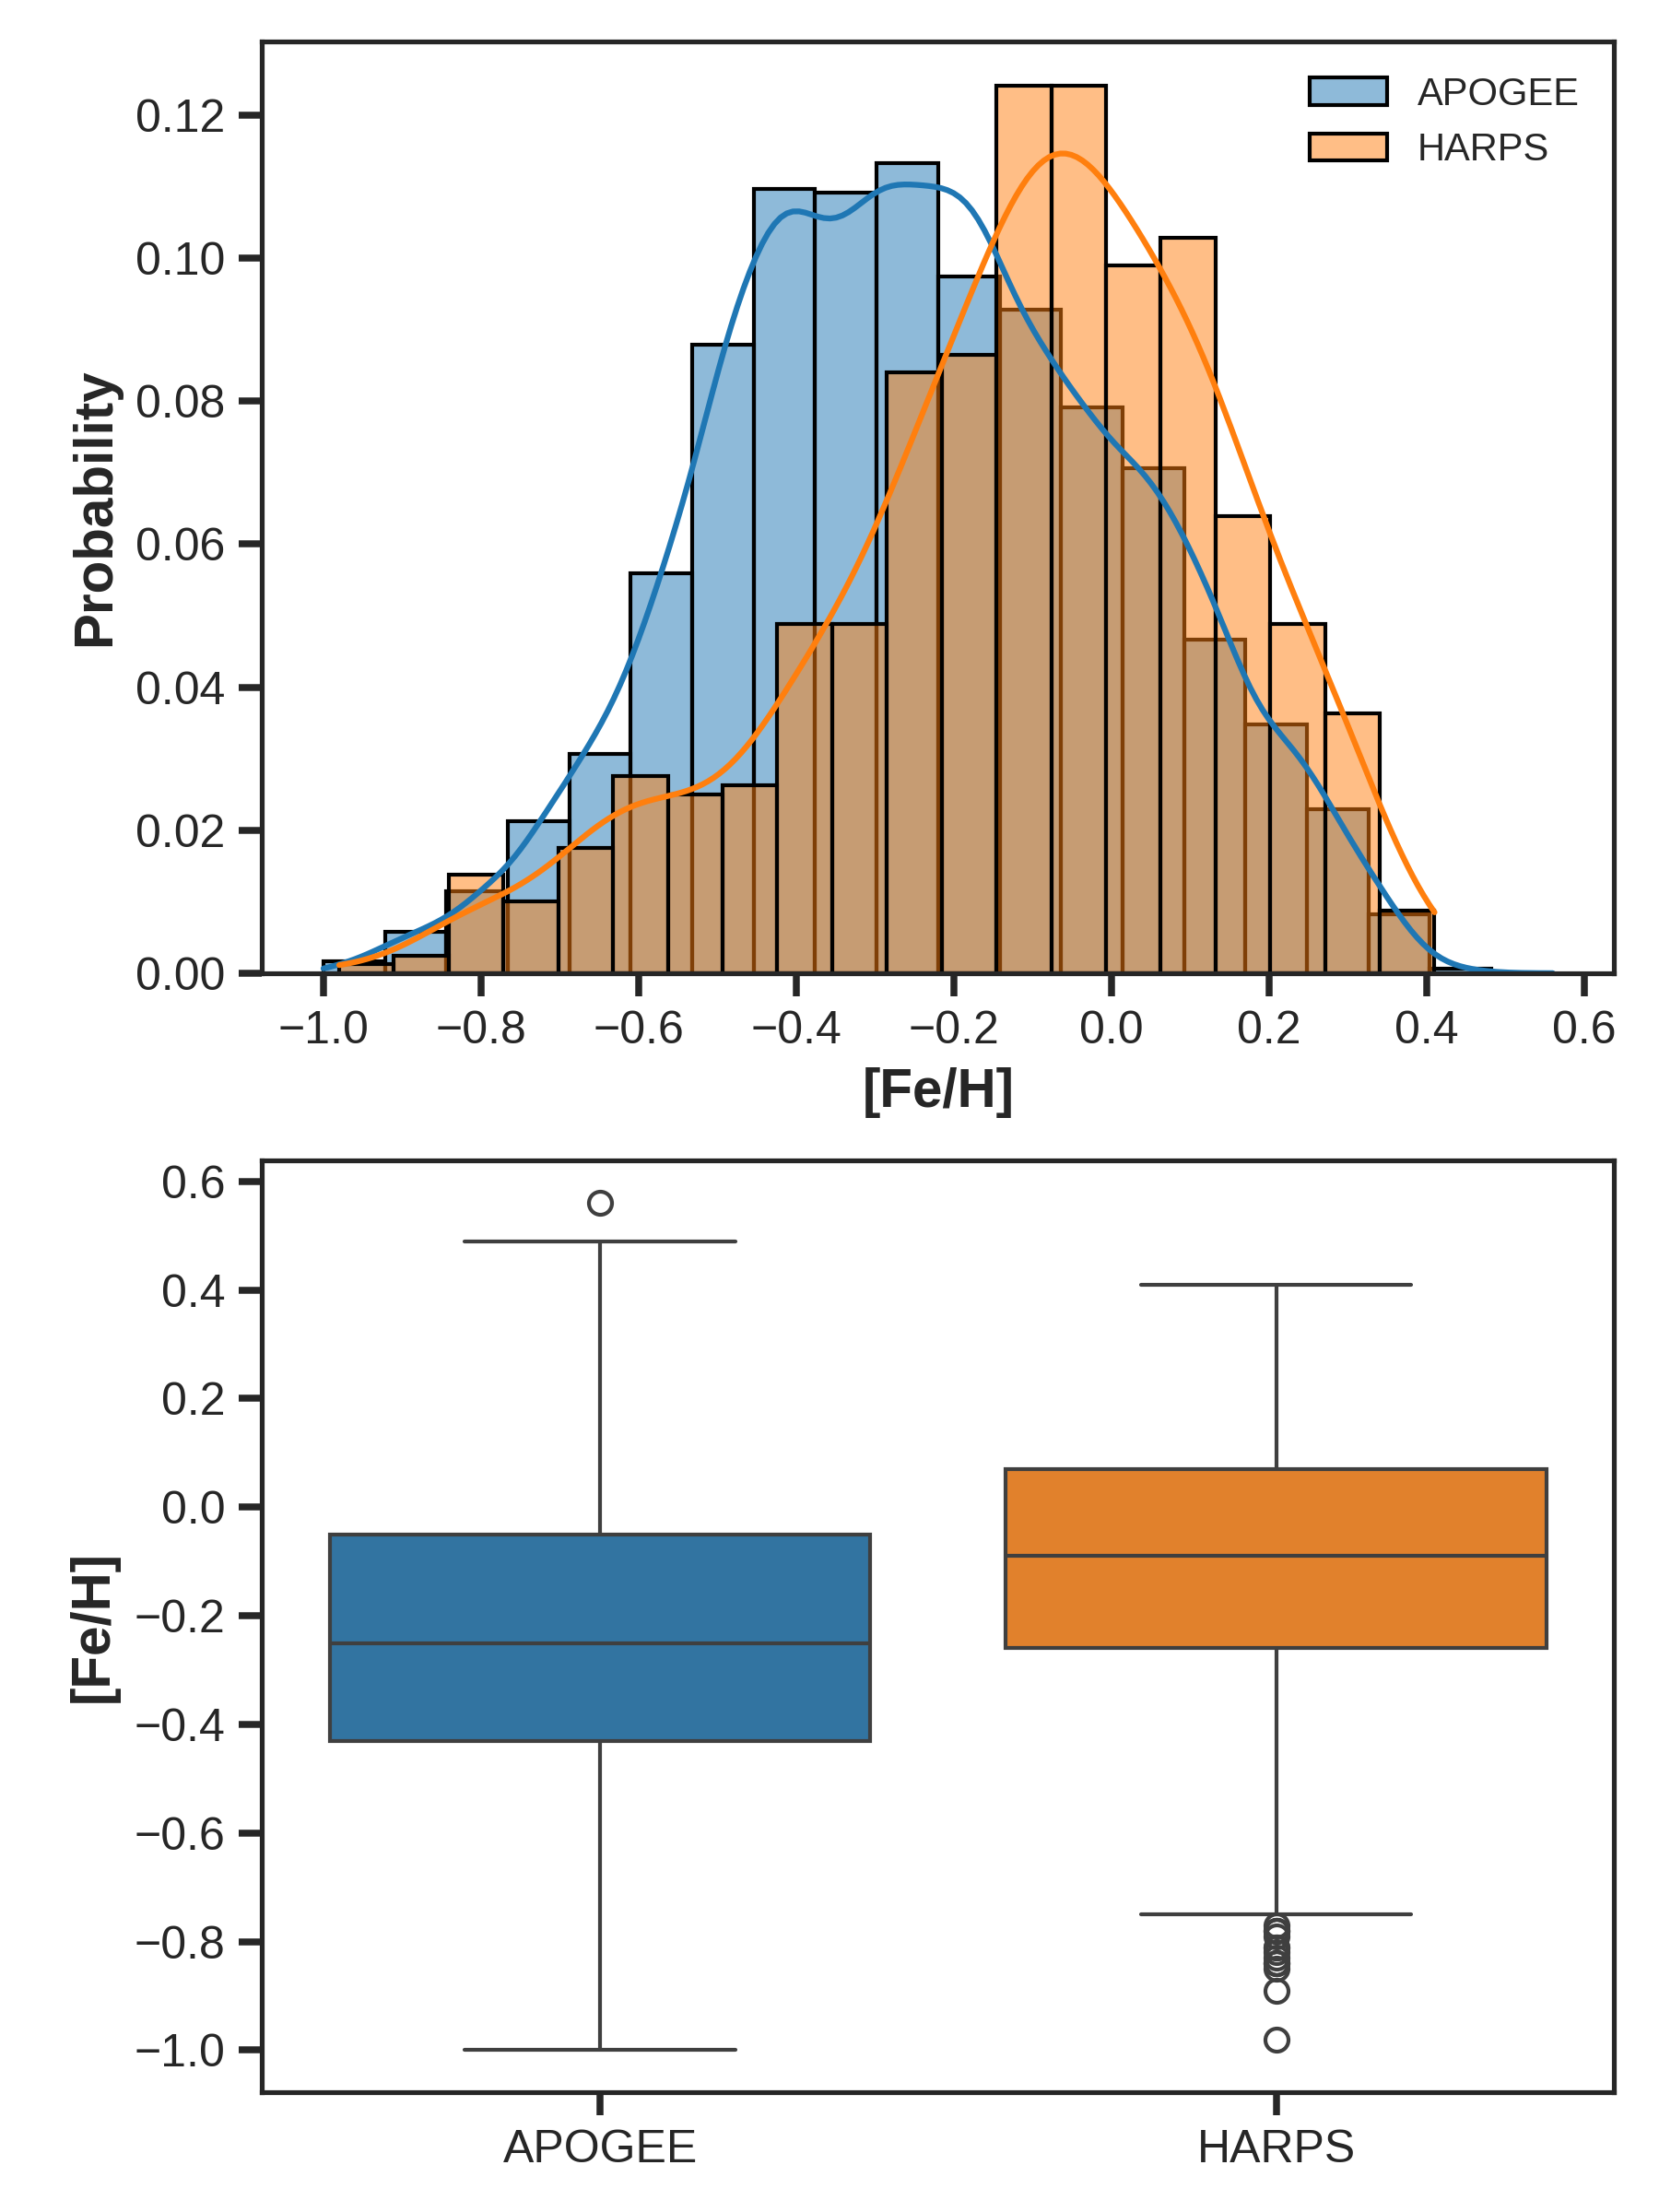
\includegraphics[width=1\linewidth]{feh_distributions_apogee_harps.png}
    \caption{
    Distributions of [Fe/H] for the two samples used in this work: APOGEE (blue)  and HARPS (green). The top panel shows the normalized probability density functions, while the bottom panel presents boxplots summarizing the median and spread of the [Fe/H] distributions.
    }
    \label{fig:feh_distributions}
\end{figure}


\section{Predicting metallicity from kinematics} \label{feh_from_kinematics}


To predict stellar metallicity, [Fe/H], we initially considered nine kinematic and orbital parameters: the Galactic velocity components ($\mathrm{U_{LSR}}$, $\mathrm{V_{LSR}}$, and $\mathrm{W_{LSR}}$), the total space velocity $\mathrm{UVW_{LSR}} = \sqrt{U_{\rm LSR}^2 + V_{\rm LSR}^2 + W_{\rm LSR}^2}$, orbital parameters derived from orbit integration (the maximum vertical excursion $Z_{\max}$, the pericentric and apocentric distances $R_{\rm peri}$ and $R_{\rm apo}$, and the orbital eccentricity $e$), and the probability of belonging to the Galactic thin-disk population, $P_{\rm gal}$.

To quantify the statistical relationships between the kinematic properties and metallicity, we evaluated monotonic correlations using Spearman’s rank coefficient \citep{spearman1904} and nonlinear dependencies using mutual information (MI). MI quantifies the general statistical dependence between two variables, including nonlinear relationships, without assuming monotonicity or linearity \citep{shannon1948}. It therefore complements Spearman’s rank coefficient and allows us to identify features that may contain predictive information beyond simple monotonic trends.

Among all parameters, $Z_{\max}$ and $P_{\rm gal}$ show the strongest correlations with metallicity, but with opposite signs. The maximum vertical excursion $Z_{\max}$ exhibits a clear negative correlation, indicating that stars reaching larger distances from the Galactic plane tend to be more metal-poor. In contrast, the thin-disk membership probability $P_{\rm gal}$ correlates positively with [Fe/H], consistent with the higher metallicities characteristic of thin-disk stars.

While some quantitative differences are observed between the APOGEE and HARPS samples—reflecting their distinct stellar populations and selection functions—the overall trends remain consistent, with $Z_{\max}$ and $P_{\rm gal}$ emerging as the dominant kinematic predictors of metallicity.

To assess multicollinearity among the input features, we computed the variance inflation factor (VIF), a standard diagnostic for linear dependence among predictors in regression analysis \citep{farrar1967}. Large VIF values indicate strong linear dependence among variables.

As expected, several parameters exhibit large VIF values. Interestingly, the two strongest predictors identified in the correlation analysis, $Z_{\max}$ and $P_{\rm gal}$, also display comparatively low VIF values, indicating that their predictive power is not merely a consequence of linear redundancy with other orbital parameters.

Although substantial multicollinearity is present (VIF $>$ 10 is typically considered as substantial), particularly among the derived velocity quantities, we retained all features in the subsequent analysis, as tree-based ensemble models are largely insensitive to correlated predictors. 


\subsection{Regression models}

We benchmarked a diverse set of regression algorithms to predict stellar metallicity from these parameters. The tested models include linear regression (LR), random forest (RF; \citealt{breiman2001}), extra trees (ET; \citealt{geurts2006}), gradient boosting methods including XGBoost \citep{chen2016}, LightGBM \citep{ke2017}, and CatBoost \citep{prokhorenkova2018}. All models were evaluated using identical $k$-fold cross-validation splits.

To provide a consistent baseline comparison, we adopted standard implementations of each algorithm with default hyperparameters and did not perform hyperparameter tuning. The goal of this experiment was to assess the intrinsic predictive power of the kinematic features
rather than to optimize individual models.

Linear regression yield RMSE values of approximately 0.21 dex. Given that the standard deviation of the metallicity distribution is $\sigma_{\rm [Fe/H]} \approx 0.26$ dex (corresponding to the RMSE of a trivial mean predictor), these models explain roughly 30\% of the total variance in [Fe/H]. This indicates that the metallicity–kinematics relation is intrinsically nonlinear. Tree-based ensemble models significantly outperform these approaches, with LightGBM achieving the lowest RMSE of $0.199 \pm 0.001$ dex ($R^2 \approx 0.41$). CatBoost and XGBoost produce nearly identical performance, while random forest and extra trees are slightly less accurate.

We further explored ensemble strategies. A weighted voting regressor combining the strongest tree-based models did not yield a measurable improvement over the best individual learner. A stacked ensemble based on out-of-fold predictions and a ridge meta-learner provided a marginal gain, reducing the RMSE only at the fourth decimal level.

This limited improvement reflects the high correlation between the predictions of the base models and indicates that performance is
primarily constrained by the information content of the kinematic features rather than by algorithmic choice.

We additionally explored a quantile-based transformation of the target variable, mapping [Fe/H] to a Gaussian distribution prior to training. While such transformations can stabilize variance and improve regression performance in skewed distributions, they did not yield any measurable improvement in our case. This result reflects both the approximately symmetric metallicity distribution
and the robustness of tree-based ensemble methods to monotonic target transformations.

Overall, the convergence of multiple algorithms, the absence of improvement from target transformation, and the limited gain from ensembling indicate that predictive performance is primarily limited by the information content of the kinematic features rather than by
model architecture.

\subsection{Exploring model architectures and feature engineering}

We performed a series of additional experiments exploring alternative modeling strategies, automated ML frameworks, and extensive feature transformations with the aim of improving the predictive performance of our models.

First, we employed two automated machine-learning frameworks, AutoGluon \citep{Erickson2020} and H2O AutoML \citep{LeDell2020}. AutoML systems automatically explore large spaces of ML pipelines by training and evaluating multiple algorithms, tuning hyperparameters, and constructing model ensembles. Such approaches are designed to approximate the best achievable performance on tabular datasets by systematically searching the model space and leveraging ensemble learning. We ran both AutoML frameworks for more than 200 hours each, allowing them to evaluate hundreds of candidate models and ensemble configurations.

Second, we investigated whether additional nonlinear interactions between the input variables could improve the predictive power. Starting from the original set of parameters, we randomly generated 300 sets of interaction features using simple algebraic transformations (multiplication, subtraction, addition, and squared terms). These engineered features were appended to the base feature set and evaluated using the tuned LightGBM model.

Third, to assess the potential impact of feature selection, we constructed 2000 random feature subsets containing between 3 and 20 parameters drawn from the expanded pool of original and engineered features. Each subset was used to train and evaluate the model in order to probe whether particular combinations of features could capture additional predictive information.

Finally, we tested whether performance could be improved by modifying the sampling of the target variable. Since extreme metallicity values are relatively underrepresented, we attempted to balance the metallicity distribution using two approaches: (i) binning the metallicity distribution and sampling more uniformly across bins, and (ii) applying sample weights to emphasize underrepresented metallicity ranges during training.

Despite these extensive experiments, all models and configurations yielded predictive performances comparable to our baseline models, with RMSE values consistently remaining above $\sim$0.198 dex. None of the explored architectures, feature transformations, feature subsets, or sampling strategies produced a measurable improvement beyond this level. This convergence strongly suggests that the achievable predictive accuracy is primarily constrained by the intrinsic information contained in the kinematic features themselves rather than by limitations of the machine-learning methodology.


\subsection{Hyperparameter optimization and final models}

Given the strong performance of gradient boosting methods in the baseline benchmark, we performed hyperparameter optimization for LightGBM and XGBoost. LightGBM was selected as the reference model based on its slightly superior performance in the default configuration, while XGBoost was included as a widely used and well-established boosting framework for tabular data applications.

The optimization was carried out using the Optuna framework \citep{Akiba-19}, which implements efficient Bayesian hyperparameter search. The tuning focused on the main parameters controlling model complexity and regularization. The objective was to minimize the cross-validated root mean squared error (RMSE) using the same five-fold splits adopted in the baseline analysis.

After optimization, both LightGBM and XGBoost achieved nearly identical predictive performance, with RMSE $\approx 0.199$ dex. The improvement relative to the default LightGBM configuration was marginal and occurred only at the third decimal level. This convergence of independently optimized models further supports the conclusion that predictive accuracy is primarily constrained by the intrinsic information content of the kinematic features rather than by the specific boosting architecture.

To assess the robustness and transferability of the trained models, we evaluated the optimized LightGBM and XGBoost models on the independent HARPS sample. The HARPS dataset has a metallicity dispersion of $\sigma_{\mathrm{[Fe/H]}} \approx 0.26$ dex, comparable to that of the APOGEE sample. Both models achieve an RMSE of approximately 0.224 dex on HARPS, corresponding to $R^2 \approx 0.26$, indicating that roughly one quarter of the metallicity variance in the HARPS sample is recovered from kinematic information alone.

It is important to note again that, although the APOGEE and HARPS samples exhibit similar metallicity dispersions, they differ in several key aspects. The mean metallicity of HARPS stars is $\langle \mathrm{[Fe/H]} \rangle = -0.115$ dex, while the APOGEE sample has a lower mean value of $-0.239$ dex. Furthermore, the two samples have distinct distributions of orbital and kinematic parameters, reflecting their different stellar populations and selection functions.


To further illustrate the performance of the LightGBM model, Fig.~\ref{fig:lgbm_apogee_harps} shows the predicted versus true metallicities and the corresponding residuals. For the APOGEE sample, the model was trained on a training subset (80\%) and evaluated on an independent test set. The upper panels of Fig.~\ref{fig:lgbm_apogee_harps} display the results for the test set. The performance of the model, trained on the full APOGEE dataset, when applied to the independent HARPS sample is shown in the lower panels of the figure.

In both datasets, the predictions exhibit a significant regression toward the mean metallicity of the training data, with metal-poor stars predicted slightly too metal-rich and metal-rich stars slightly underestimated. This behaviour reflects the well-known phenomenon of regression toward the mean \citep{Galton-1886} and arises naturally when the predictors do not fully constrain the target variable. Under a squared-error loss function, the optimal prediction in the presence of incomplete information is biased toward the conditional mean of the target \citep{Hastie2009}. In this case, the limited information content of the kinematic features results in a reduced dynamic range of the predictions relative to the true metallicity distribution.

\begin{figure}[ht]
\centering
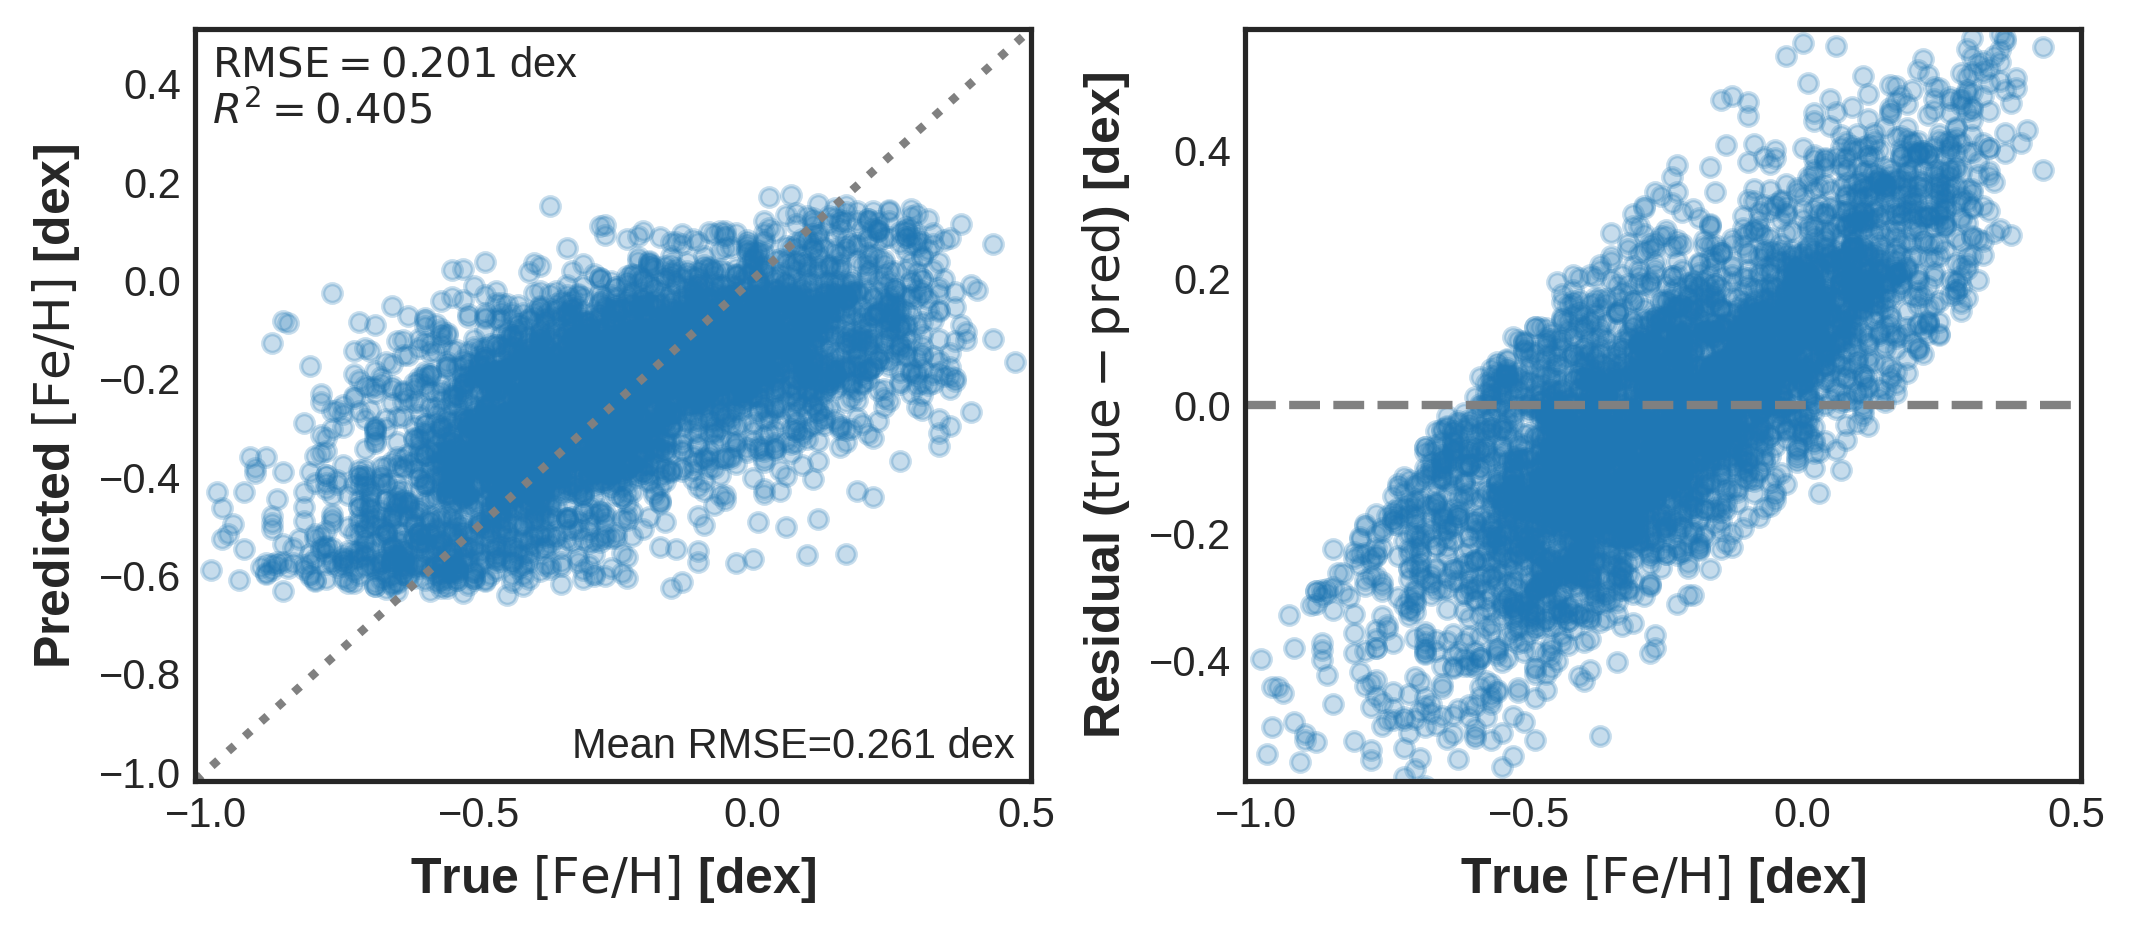
\includegraphics[width=\linewidth]{figures/fig_apogee_lgbm_pred_resid_scatter.png}
\vfill
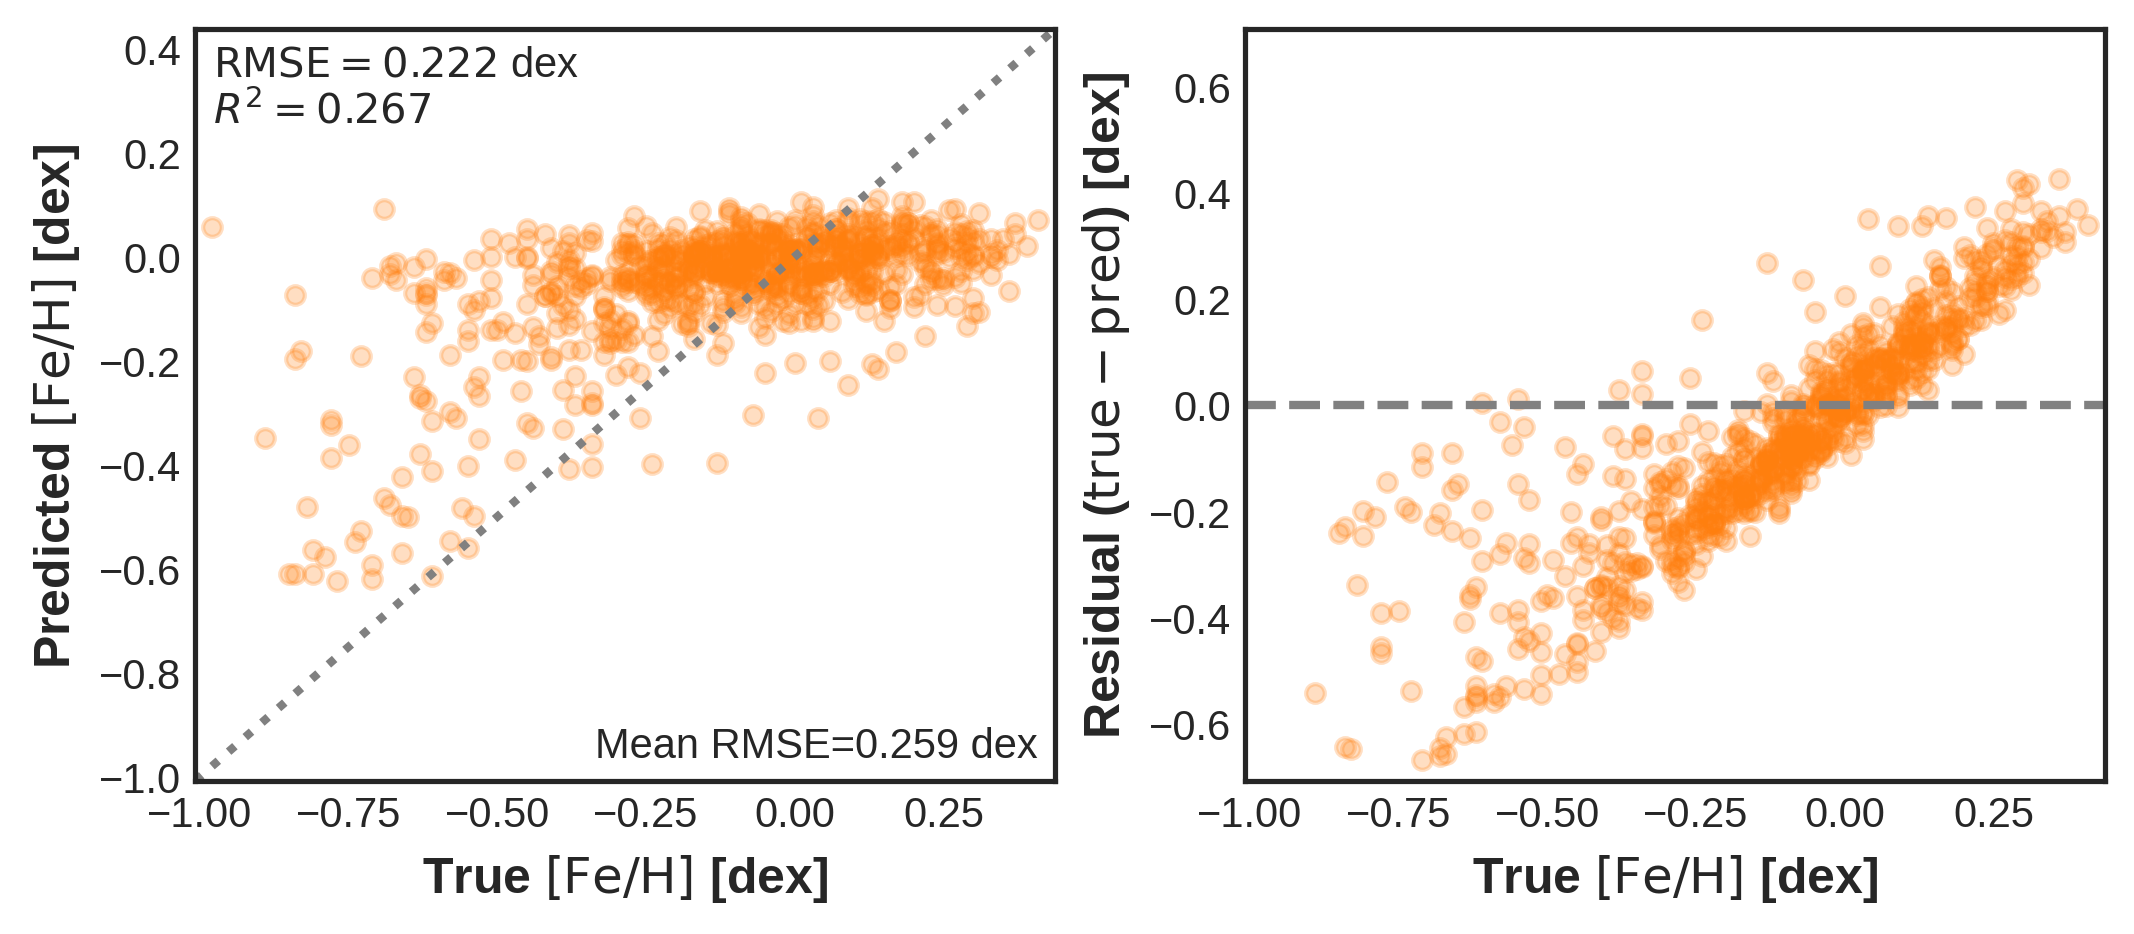
\includegraphics[width=\linewidth]{figures/fig_harps_lgbm_pred_resid_scatter.png}
\caption{Performance of the tuned LightGBM model for metallicity prediction. Top panels: APOGEE test set results. Bottom panels: HARPS results. Left panels show predicted versus true metallicity with the one-to-one relation indicated by the dotted line. Right panels show residuals as a function of true metallicity.}
\label{fig:lgbm_apogee_harps}
\end{figure}


\subsection{Feature importance analysis} \label{main_feat_imp_feh}

To quantify the relative contribution of each kinematic parameter to the metallicity prediction, we performed a comprehensive feature importance analysis using four complementary approaches: built-in gain-based importance, permutation importance \citep{breiman2001}, single-feature predictive performance, and SHAP values \citep{Lundberg-17, Lundberg2020}. Figures are shown in Sect.~\ref{appendix:feature_importance_feh}.

For LightGBM and XGBoost we first considered the built-in feature importance based on the total gain. In tree-based ensembles, the gain measures the total reduction in the loss function (in our case, squared error) produced by splits involving a given feature across all trees in the ensemble. Larger gain values therefore indicate that a feature contributes more strongly to improving model accuracy. Although gain importance is model-dependent and not directly comparable across algorithms, it provides an initial ranking of influential parameters.

In both models, $Z_{\max}$ clearly dominates the ranking, followed by $R_{\mathrm{apo}}$, $R_{\mathrm{peri}}$, and the orbital eccentricity $e$. Galactic space velocity components ($U_{\mathrm{LSR}}$, $V_{\mathrm{LSR}}$, $W_{\mathrm{LSR}}$, and $UVW_{\mathrm{LSR}}$) and $P_{\mathrm{gal}}$ contribute substantially less to the predictive power.


To obtain a model-agnostic estimate of feature relevance, we computed permutation importance. This method evaluates the increase in prediction error when the values of a single feature are randomly shuffled, thereby breaking its statistical relationship with the target variable. The importance is quantified as the change in cross-validated RMSE ($\Delta \mathrm{RMSE}$).

Permutation importance confirms the dominance of $Z_{\max}$, which produces by far the largest degradation in performance when permuted. The next most important parameters are $R_{\mathrm{apo}}$ and $R_{\mathrm{peri}}$, followed by eccentricity.

As an additional diagnostic, we trained each model using only one feature at a time and computed the cross-validated RMSE. This approach quantifies the intrinsic predictive power of each parameter in isolation. Using $Z_{\max}$ alone yields an RMSE of $\sim 0.22$ dex, significantly better than any other single parameter. All other features individually result in RMSE values above $0.24$ dex.

To further investigate both global importance and the direction of feature effects, we computed SHAP (SHapley Additive exPlanations) values for the tuned models. SHAP values decompose each individual prediction into additive contributions from each feature, grounded in cooperative game theory. The global importance of a feature is quantified as the mean absolute SHAP value, $\langle |\mathrm{SHAP}| \rangle$.

Across the two models, the SHAP rankings are remarkably consistent. $Z_{\max}$ exhibits the largest mean absolute contribution, followed by $R_{\mathrm{apo}}$ and $R_{\mathrm{peri}}$. Eccentricity contributes at an intermediate level, while the velocity components have substantially smaller SHAP amplitudes.

All four importance diagnostics consistently identify the same ranking of parameters across LightGBM and XGBoost. The convergence of independent models and independent importance measures indicates that the result is robust and not an artifact of a specific boosting architecture.

In summary, the metallicity–kinematics relation is primarily driven by vertical orbital structure ($Z_{\max}$), with additional contributions from radial orbital extent ($R_{\mathrm{apo}}$ and $R_{\mathrm{peri}}$) and eccentricity. Instantaneous velocity components and the thin-disk membership probability $P_{\rm gal}$ add comparatively little independent information once orbital parameters are included.

\subsection{\texorpdfstring{The $Z_{\max}$--metallicity relation}{The Zmax-metallicity relation}}

Given the dominant role of $Z_{\max}$ in all feature-importance diagnostics, we further examine its detailed relation with metallicity using SHAP dependence plots (Fig.~\ref{fig:shap_zmax_apogee_harps}). These plots show the SHAP contribution of $Z_{\max}$ to the predicted metallicity as a function of its physical value, with points color-coded by apocentric distance $R_{\mathrm{apo}}$ and thin-disk membership probability $P_{\rm gal}$.

\begin{figure}[ht]
\centering
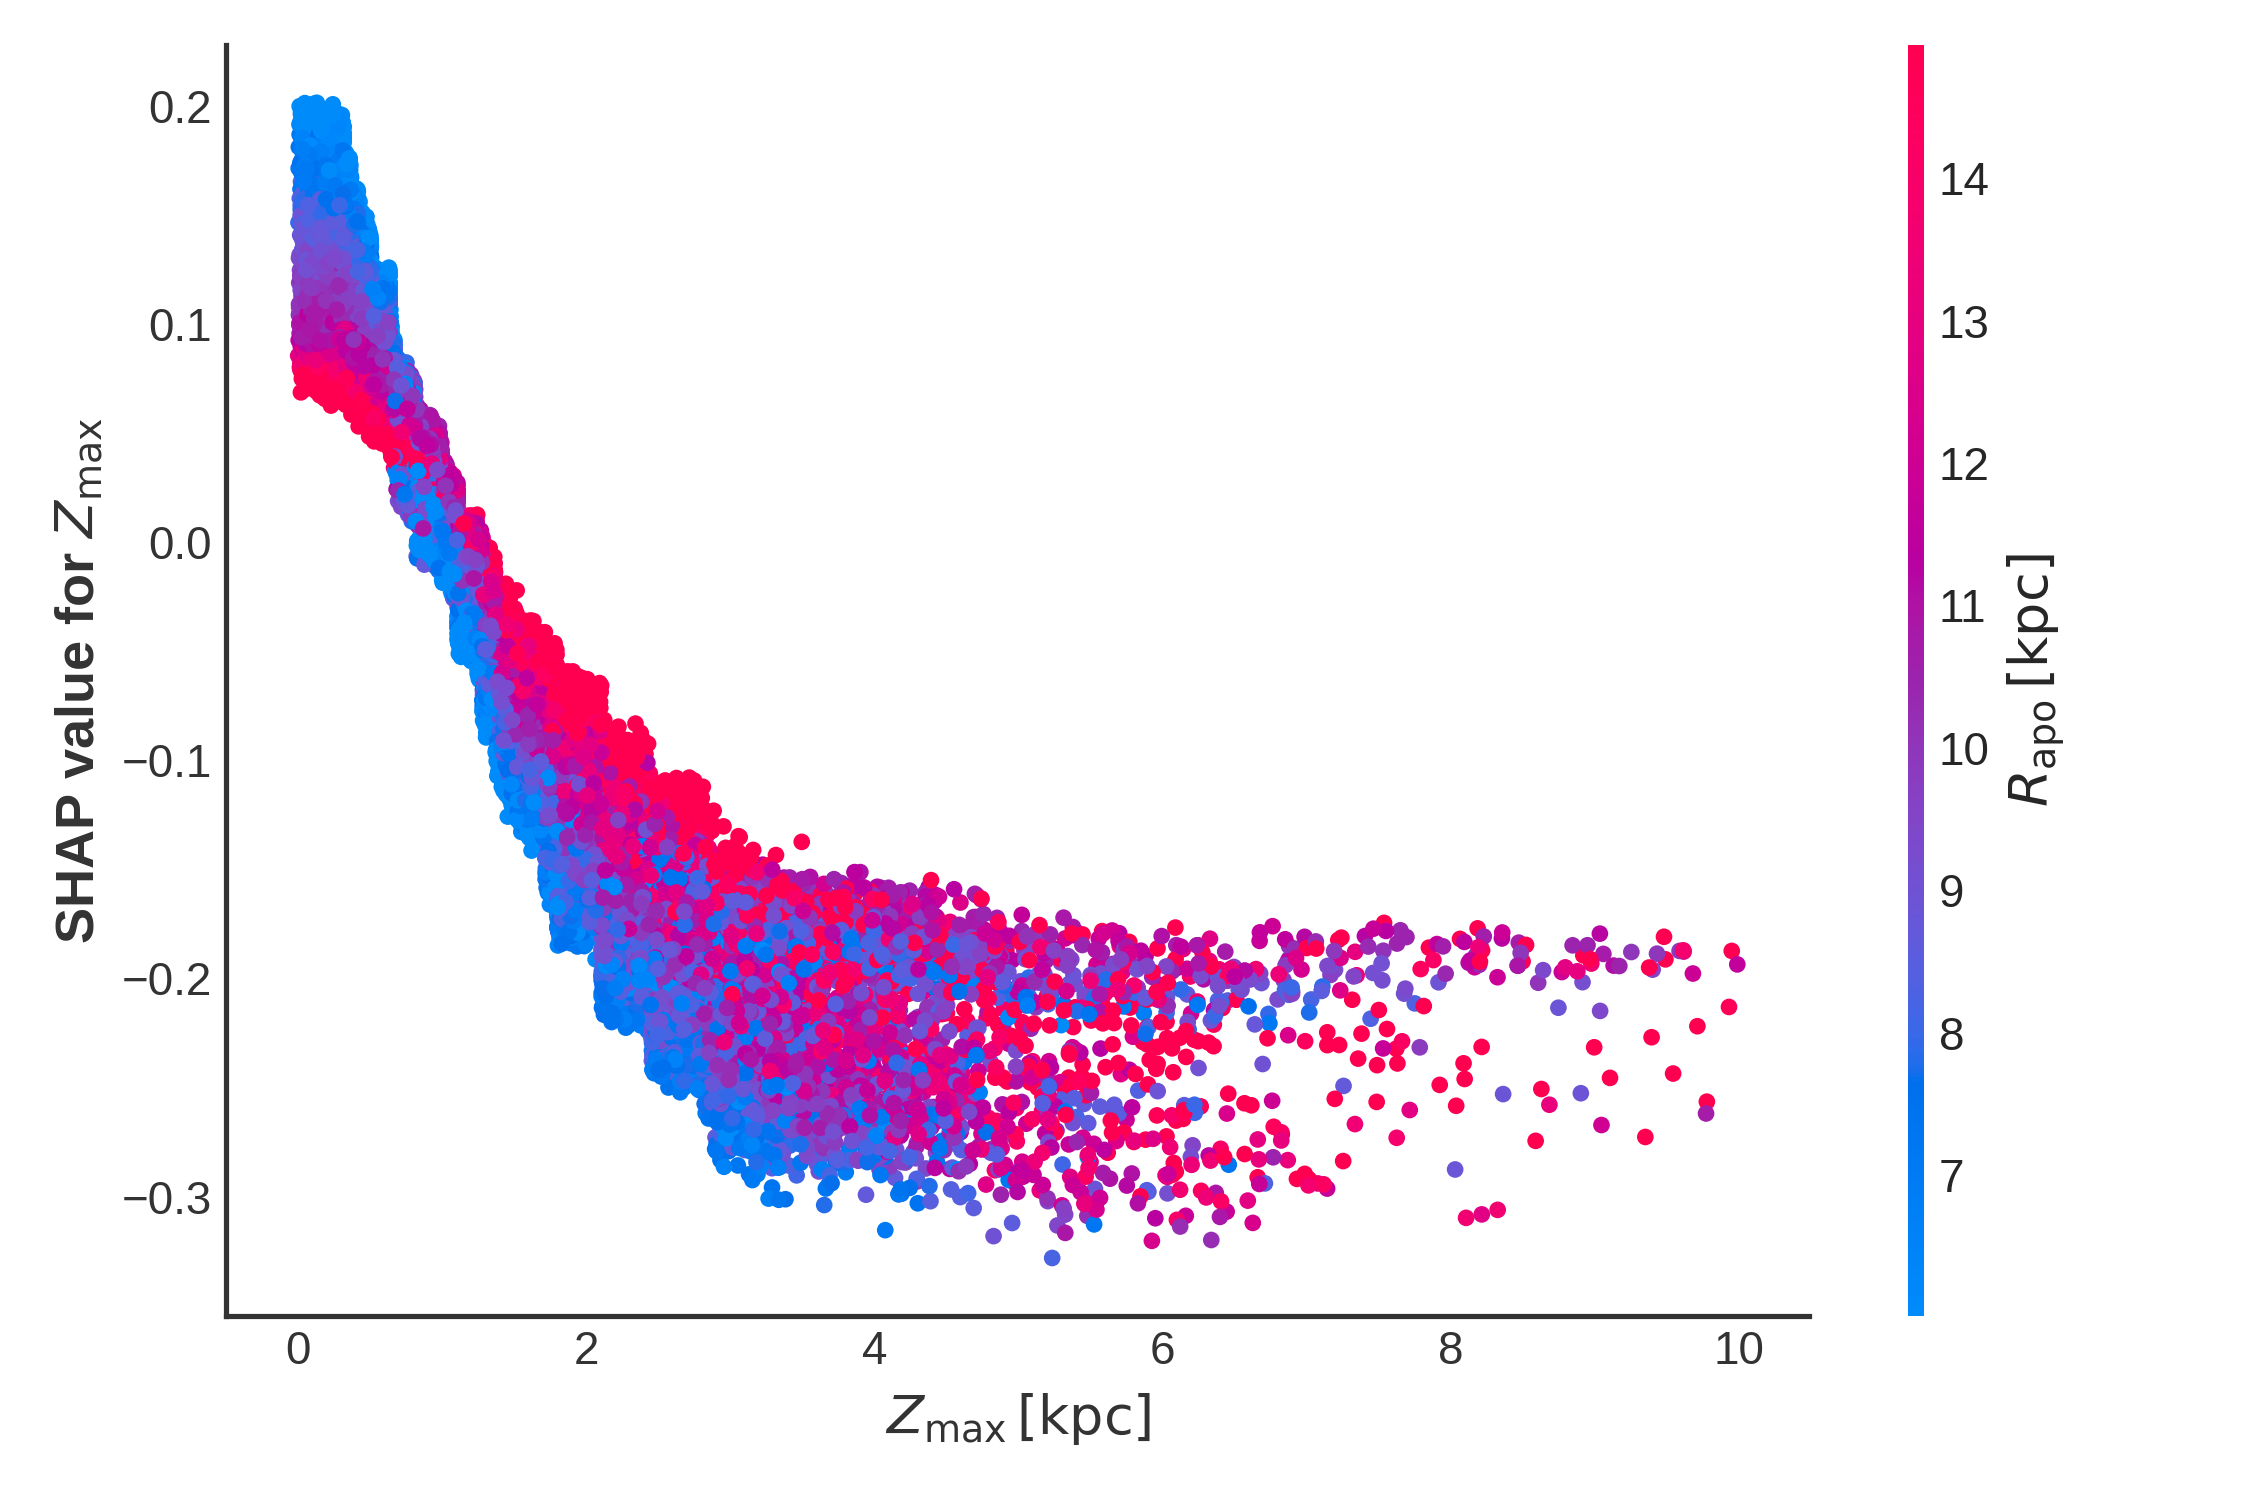
\includegraphics[width=\linewidth]{figures/LGBM_zmax_rapo_dependence_pretty.png}
\vfill
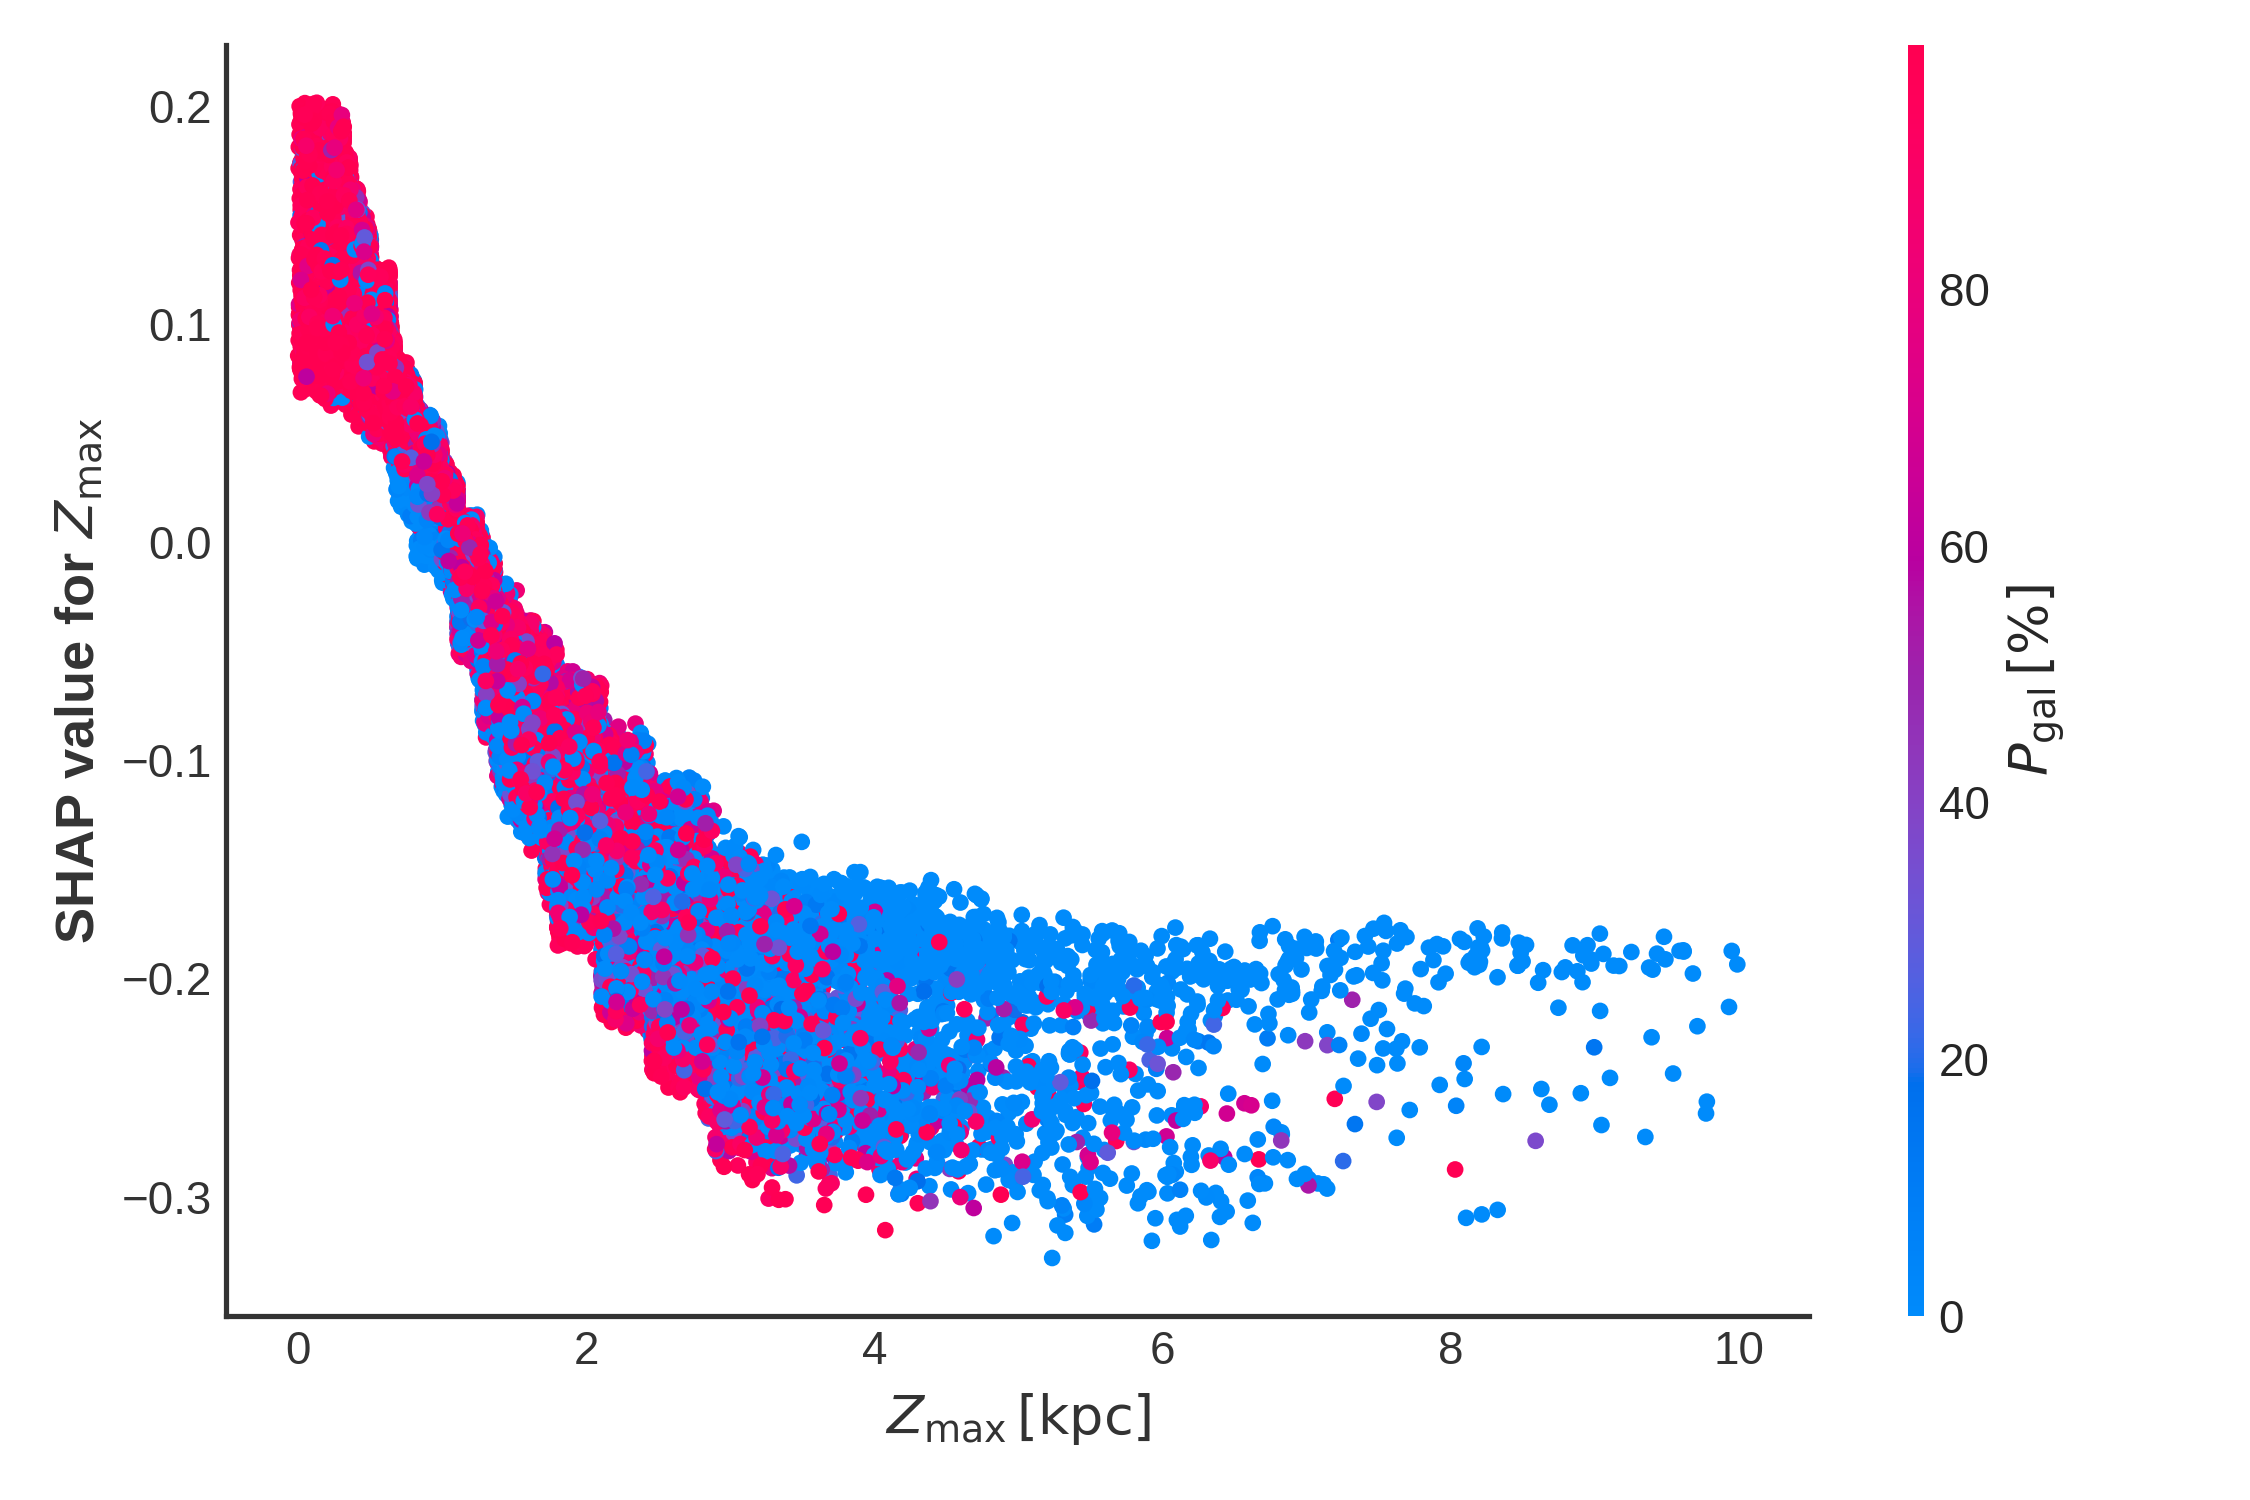
\includegraphics[width=\linewidth]{figures/LGBM_zmax_pgal_dependence_pretty.png}
\caption{SHAP dependence of $Z_{\max}$ for the tuned LightGBM model. The vertical axis shows the SHAP contribution of $Z_{\max}$ to the predicted metallicity, while the horizontal axis shows its physical value in kpc. Points are color-coded by apocentric radius $R_{\mathrm{apo}}$ (top panel) and by their thin-disk membership probability $P_{\rm gal}$ (bottom panel).}
\label{fig:shap_zmax_apogee_harps}
\end{figure}

For the APOGEE sample, the SHAP dependence plot reveals a strong and monotonic decrease of the SHAP contribution of $Z_{\max}$ with increasing $Z_{\max}$. Since SHAP values quantify the shift of the prediction relative to the global mean metallicity of the training data, positive values indicate that $Z_{\max}$ increases the predicted metallicity, while negative values indicate that it decreases it. Stars confined close to the Galactic plane ($Z_{\max} \lesssim 1$ kpc) therefore tend to have their predicted metallicities shifted upward relative to the mean, whereas stars reaching large vertical distances shift the prediction downward.

The relation steepens at small $Z_{\max}$ and gradually flattens beyond $\sim$3–4 kpc. Interestingly, the dispersion of SHAP values becomes minimal and approaches zero around $Z_{\max} \sim 1$–1.5 kpc. This indicates a regime in which the vertical orbital extent alone does not strongly bias the prediction relative to the mean metallicity, and where additional orbital parameters begin to modulate the metallicity more significantly. At larger $Z_{\max}$, the increasing dispersion reflects a broader range of metallicities among dynamically hotter populations, consistent with a transition from thin-disk dominated stars to thick-disk and kinematically heated components.

The color-coding by $R_{\mathrm{apo}}$ suggests a secondary modulation by radial orbital extent. At small $Z_{\max}$, stars with larger apocentric distances tend to show slightly more negative SHAP contributions, indicating lower predicted metallicities. Beyond $Z_{\max} \sim 1$ kpc, this trend weakens and partially reverses, suggesting that the coupling between vertical and radial orbital properties changes across disk populations. We regard this secondary trend as suggestive rather than definitive, but it is broadly consistent with a changing mixture of thin- and thick-disk stars across the $Z_{\max}$ sequence.

Overall, this analysis indicates that vertical orbital extent provides the primary dynamical imprint on metallicity, while radial orbital properties introduce a secondary, population-dependent modulation. Such behaviour is consistent with expectations from Galactic chemo-dynamical evolution, in which dynamically hotter and more radially extended stellar populations are typically older and more metal-poor.


\section{Predicting individual abundances from [Fe/H] and kinematics}

We next investigate whether the abundances of individual elements can be predicted from stellar metallicity combined with kinematic information. We focus on C, O, Mg, and Si, which are of particular interest for exoplanet studies and especially relevant for M-dwarf applications, where reliable determinations of individual elemental abundances are far more difficult than measurements of the overall metallicity.

For each element we first explored which parameters are most strongly associated with its abundance by computing both Spearman's rank correlation coefficient and the MI between the abundance and the input features. For the APOGEE sample, the strongest correlation is found with [Fe/H], as expected from the Galactic chemical evolution, with typical Spearman coefficients of $\rho \sim 0.9$ for all considered elements. The next most informative parameters are related to the stellar orbital properties, in particular $Z_{\max}$, $R_{\mathrm{apo}}$, and $R_{\mathrm{peri}}$, with correlation coefficients typically in the range $0.2 \lesssim \rho \lesssim 0.4$. The MI analysis reveals a very similar picture, indicating that the dominant information about the elemental abundances is carried by [Fe/H], while the orbital parameters provide secondary but non-negligible contributions.

For the HARPS sample, stellar metallicity remains the dominant parameter, with both $\rho$ and MI values significantly larger than those of the remaining features. Among the other parameters, $Z_{\max}$ and $P_{\mathrm{gal}}$ show the strongest associations with the elemental abundances, with typical Spearman coefficients of $\rho \approx -0.2$ and $\rho \approx 0.2$, respectively.

The full set of Spearman correlation and mutual information diagrams for all considered elements is presented in Appendix~\ref{appendix:correlations_mi_abund}.


\subsection{Regression models}

Using the same framework as for metallicity prediction, we benchmarked a broad set of ML regressors to estimate the abundances of C, O, Mg, and Si from stellar metallicity and kinematics. The models were evaluated with five-fold cross-validation on the APOGEE training sample using the same metrics as before (RMSE, MAE, and $R^2$). The complete set of results is presented in Table~\ref{tab:abundance_cv_scores}.

Overall, the behaviour of the different algorithms is very similar to that found for the metallicity prediction task. Among the considered models, gradient boosting methods consistently provide the best performance without requiring hyperparameter tuning. In particular, the LightGBM and CatBoost regressors achieve the lowest prediction errors for all elements. Given its consistently high predictive performance across all considered elements and its computational efficiency, we adopt the LightGBM regressor as the primary model for the subsequent analysis.

We optimised hyperparameters of LightGBM using Optuna. For each elemental abundance ([C/H], [O/H], [Mg/H], and [Si/H]) the hyperparameters of the LightGBM model were optimised using the APOGEE training sample. The tuned models show only modest improvements relative to the models trained with default parameters. After determining the optimal hyperparameters, the final models were trained using the full APOGEE dataset and subsequently applied to the independent HARPS sample.

Table~\ref{tab:abundance_predictions} summarises the prediction accuracy for both the APOGEE holdout sample and the HARPS dataset. For comparison, we also report the RMSE obtained with a simple baseline predictor assuming that the abundance of a given element is equal to the stellar metallicity (i.e. $\mathrm{[X/H]} = \mathrm{[Fe/H]}$). This baseline model represents the scenario in which no additional information beyond metallicity is used. The results demonstrate that incorporating kinematic information significantly improves the prediction accuracy for all elements relative to this simple approximation.

\begin{table}
\caption{Prediction accuracy of the tuned LightGBM models for elemental abundances.
The APOGEE results correspond to the holdout validation sample, while the HARPS
results represent predictions for the independent test dataset. For comparison,
the RMSE values obtained from a baseline predictor assuming
$\mathrm{[X/H]}=\mathrm{[Fe/H]}$ are also shown.}
\centering
\begin{tabular}{lcccc}
\hline
 & [O/H] & [Mg/H] & [Si/H] & [C/H] \\
\hline
RMSE$_{\mathrm{APOGEE}}$ & 0.054 & 0.049 & 0.037 & 0.080 \\
RMSE$_{\mathrm{HARPS}}$  & 0.098 & 0.070 & 0.043 & 0.097 \\
\hline
RMSE$_{\mathrm{[Fe/H]}}$ (APOGEE) & 0.192 & 0.175 & 0.119 & 0.116 \\
RMSE$_{\mathrm{[Fe/H]}}$ (HARPS)  & 0.170 & 0.107 & 0.078 & 0.106 \\
\hline
\end{tabular}
\label{tab:abundance_predictions}
\end{table}

Figure~\ref{fig:abundance_predictions} illustrates the performance of the tuned models for both the APOGEE holdout sample and the HARPS dataset. The left panels show the predicted abundance ratios as a function of metallicity, compared with the true stellar abundances. The predicted values closely follow the global trends expected from Galactic chemical evolution.

However, it is also evident that the predictions become less reliable at the extremes of the metallicity distribution. In particular, stars with $\mathrm{[Fe/H]} < -0.8$ dex and $\mathrm{[Fe/H]} > 0.35$ dex show larger deviations between predicted and true abundances. This behaviour is primarily driven by the scarcity of training data in these metallicity regimes. To focus on the regime where the models are most reliable, the residual distributions shown in the right panels are restricted to stars within the metallicity interval $-0.8 < \mathrm{[Fe/H]} < 0.35$ dex.

Overall, the models reproduce the main Galactic chemical evolution trends remarkably well for all elements considered. Nevertheless, the residual panels reveal small systematic trends, indicating that the models do not fully capture the detailed abundance behaviour across the entire metallicity range. These residual structures likely reflect both the intrinsic complexity of Galactic chemical evolution and the limited information contained in the kinematic features used as predictors.

When applying the trained models to the HARPS dataset, we observe a systematic offset between the predicted and true [C/H] abundances. This discrepancy reflects intrinsic differences between the APOGEE and HARPS samples. In particular, at a given metallicity, APOGEE stars exhibit [C/Fe] abundances that are lower by approximately 0.1 dex compared to those in the HARPS sample. After accounting for this offset by applying a constant correction to the predicted values, the RMSE of the [C/H] predictions decreases significantly, reaching $\sim$0.08 dex. This result indicates that the dominant source of the discrepancy is not a limitation of the model itself, but rather a systematic difference in the abundance scales between the two datasets.

\begin{figure*}
\centering
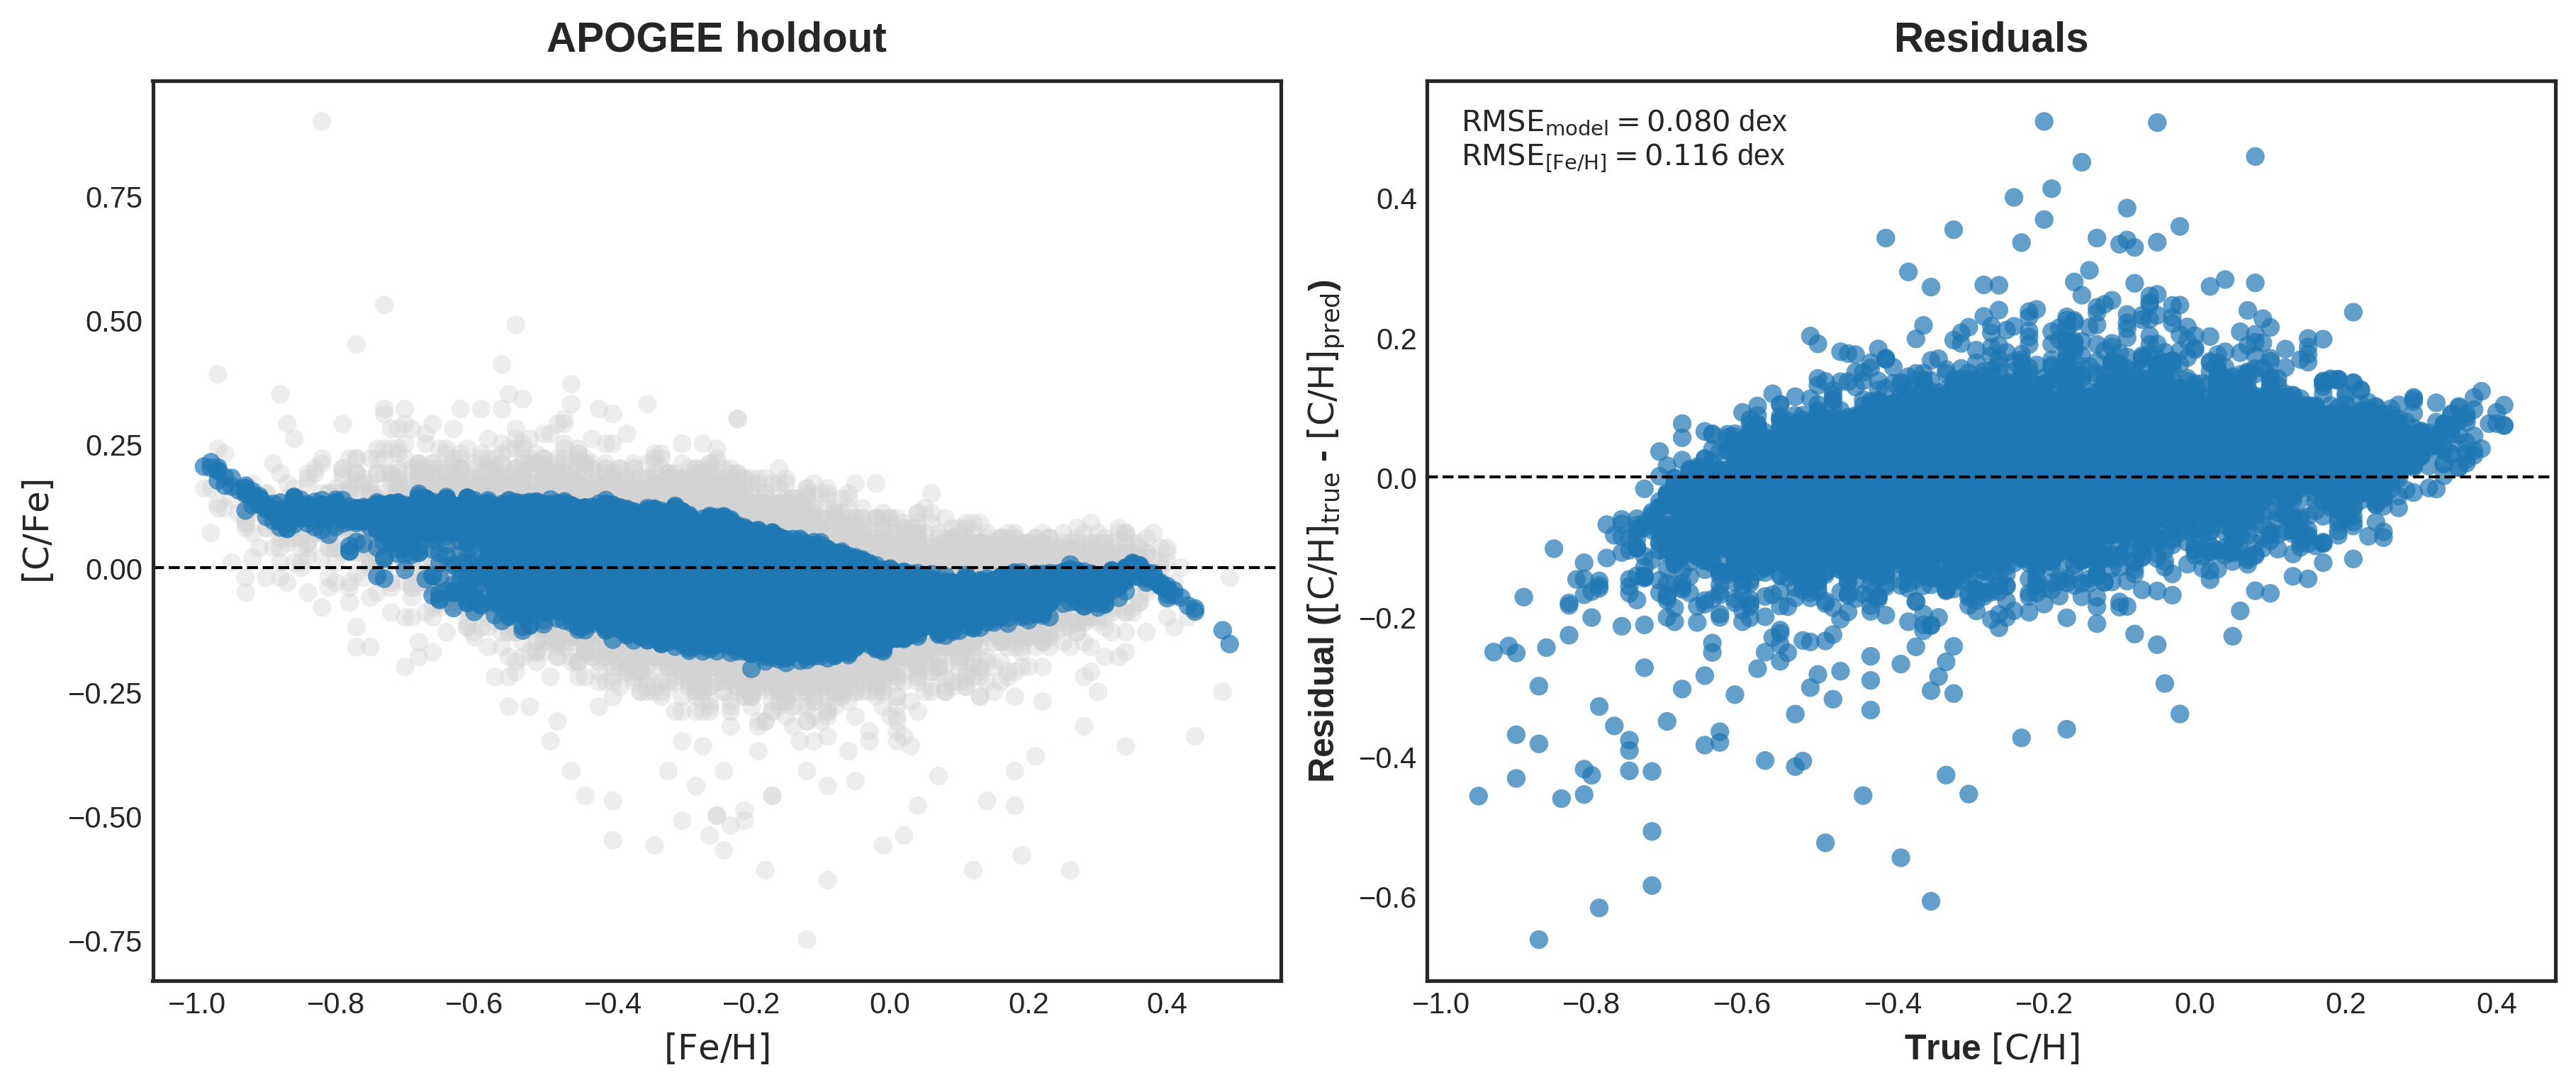
\includegraphics[width=0.48\textwidth]{figures/c_h_apogee_holdout.png}
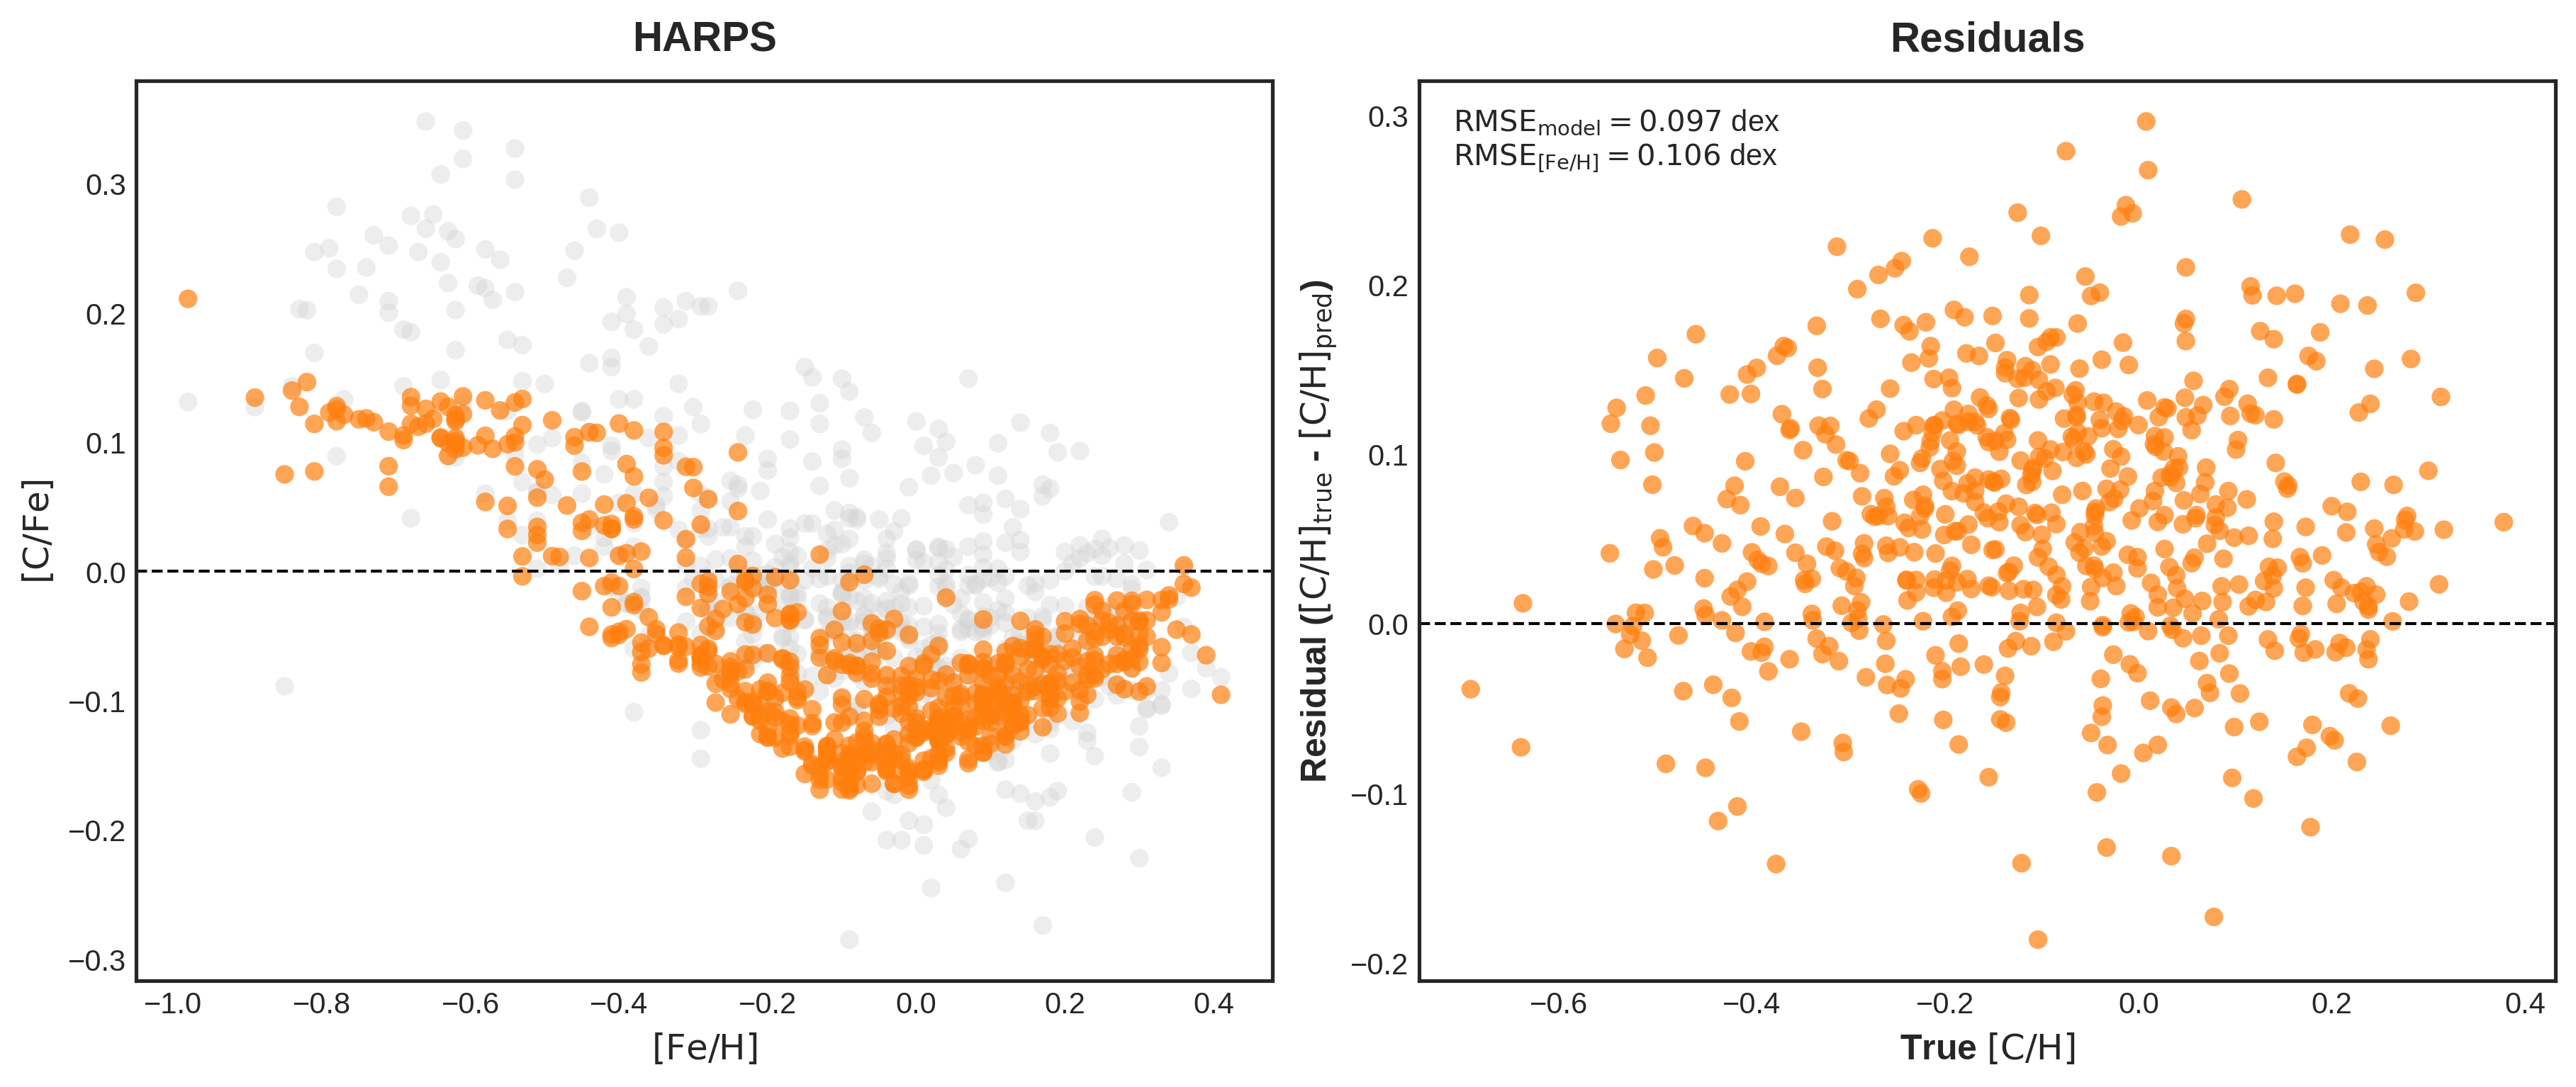
\includegraphics[width=0.48\textwidth]{figures/c_h_harps.png}
\hfill
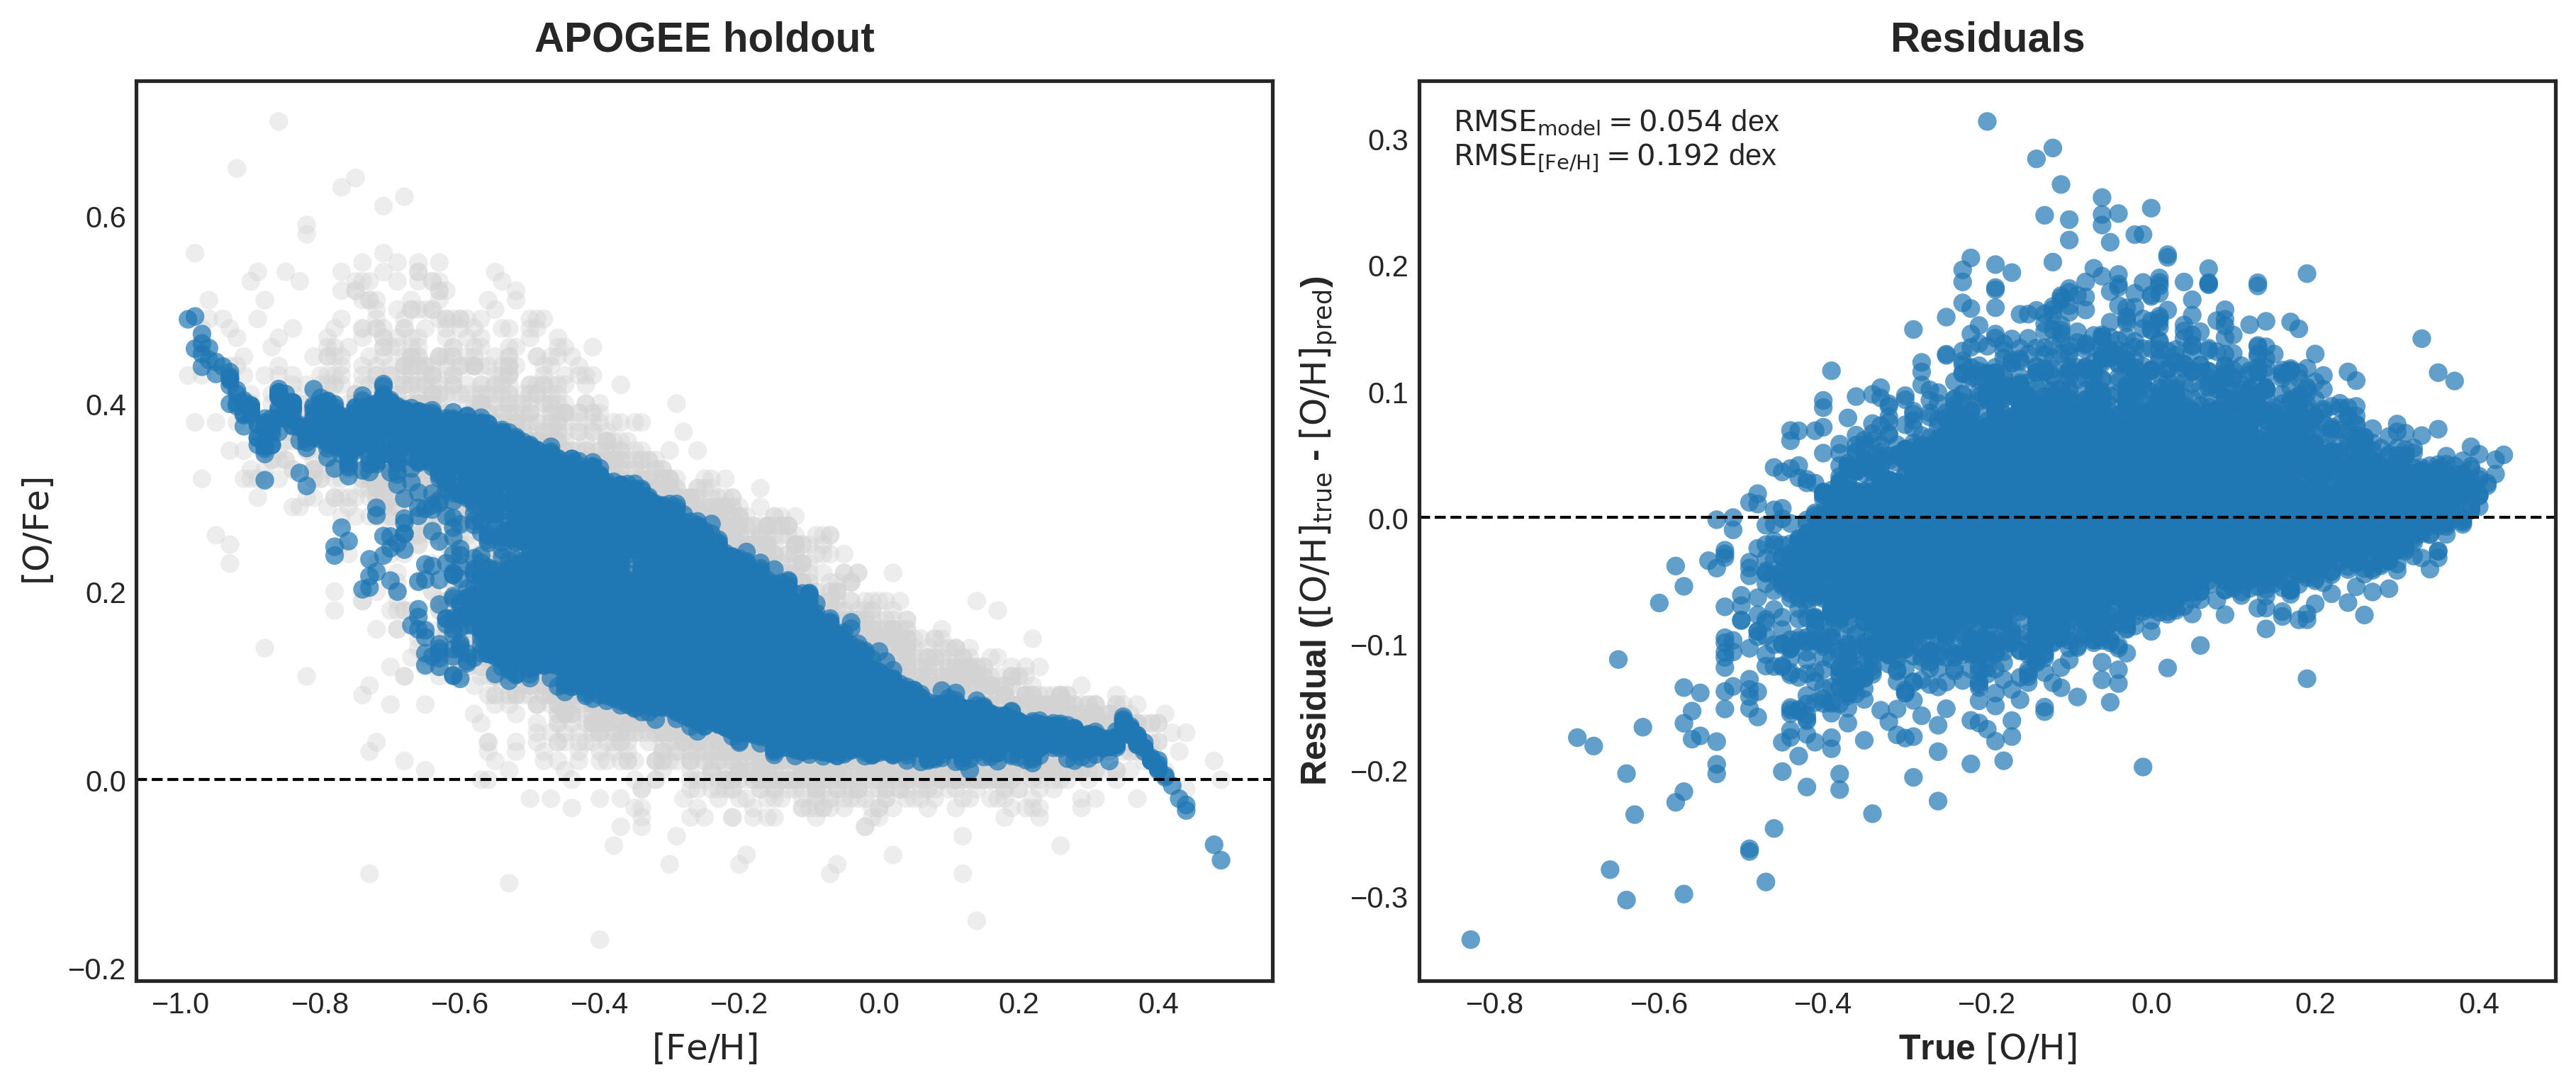
\includegraphics[width=0.48\textwidth]{figures/o_h_apogee_holdout.png}
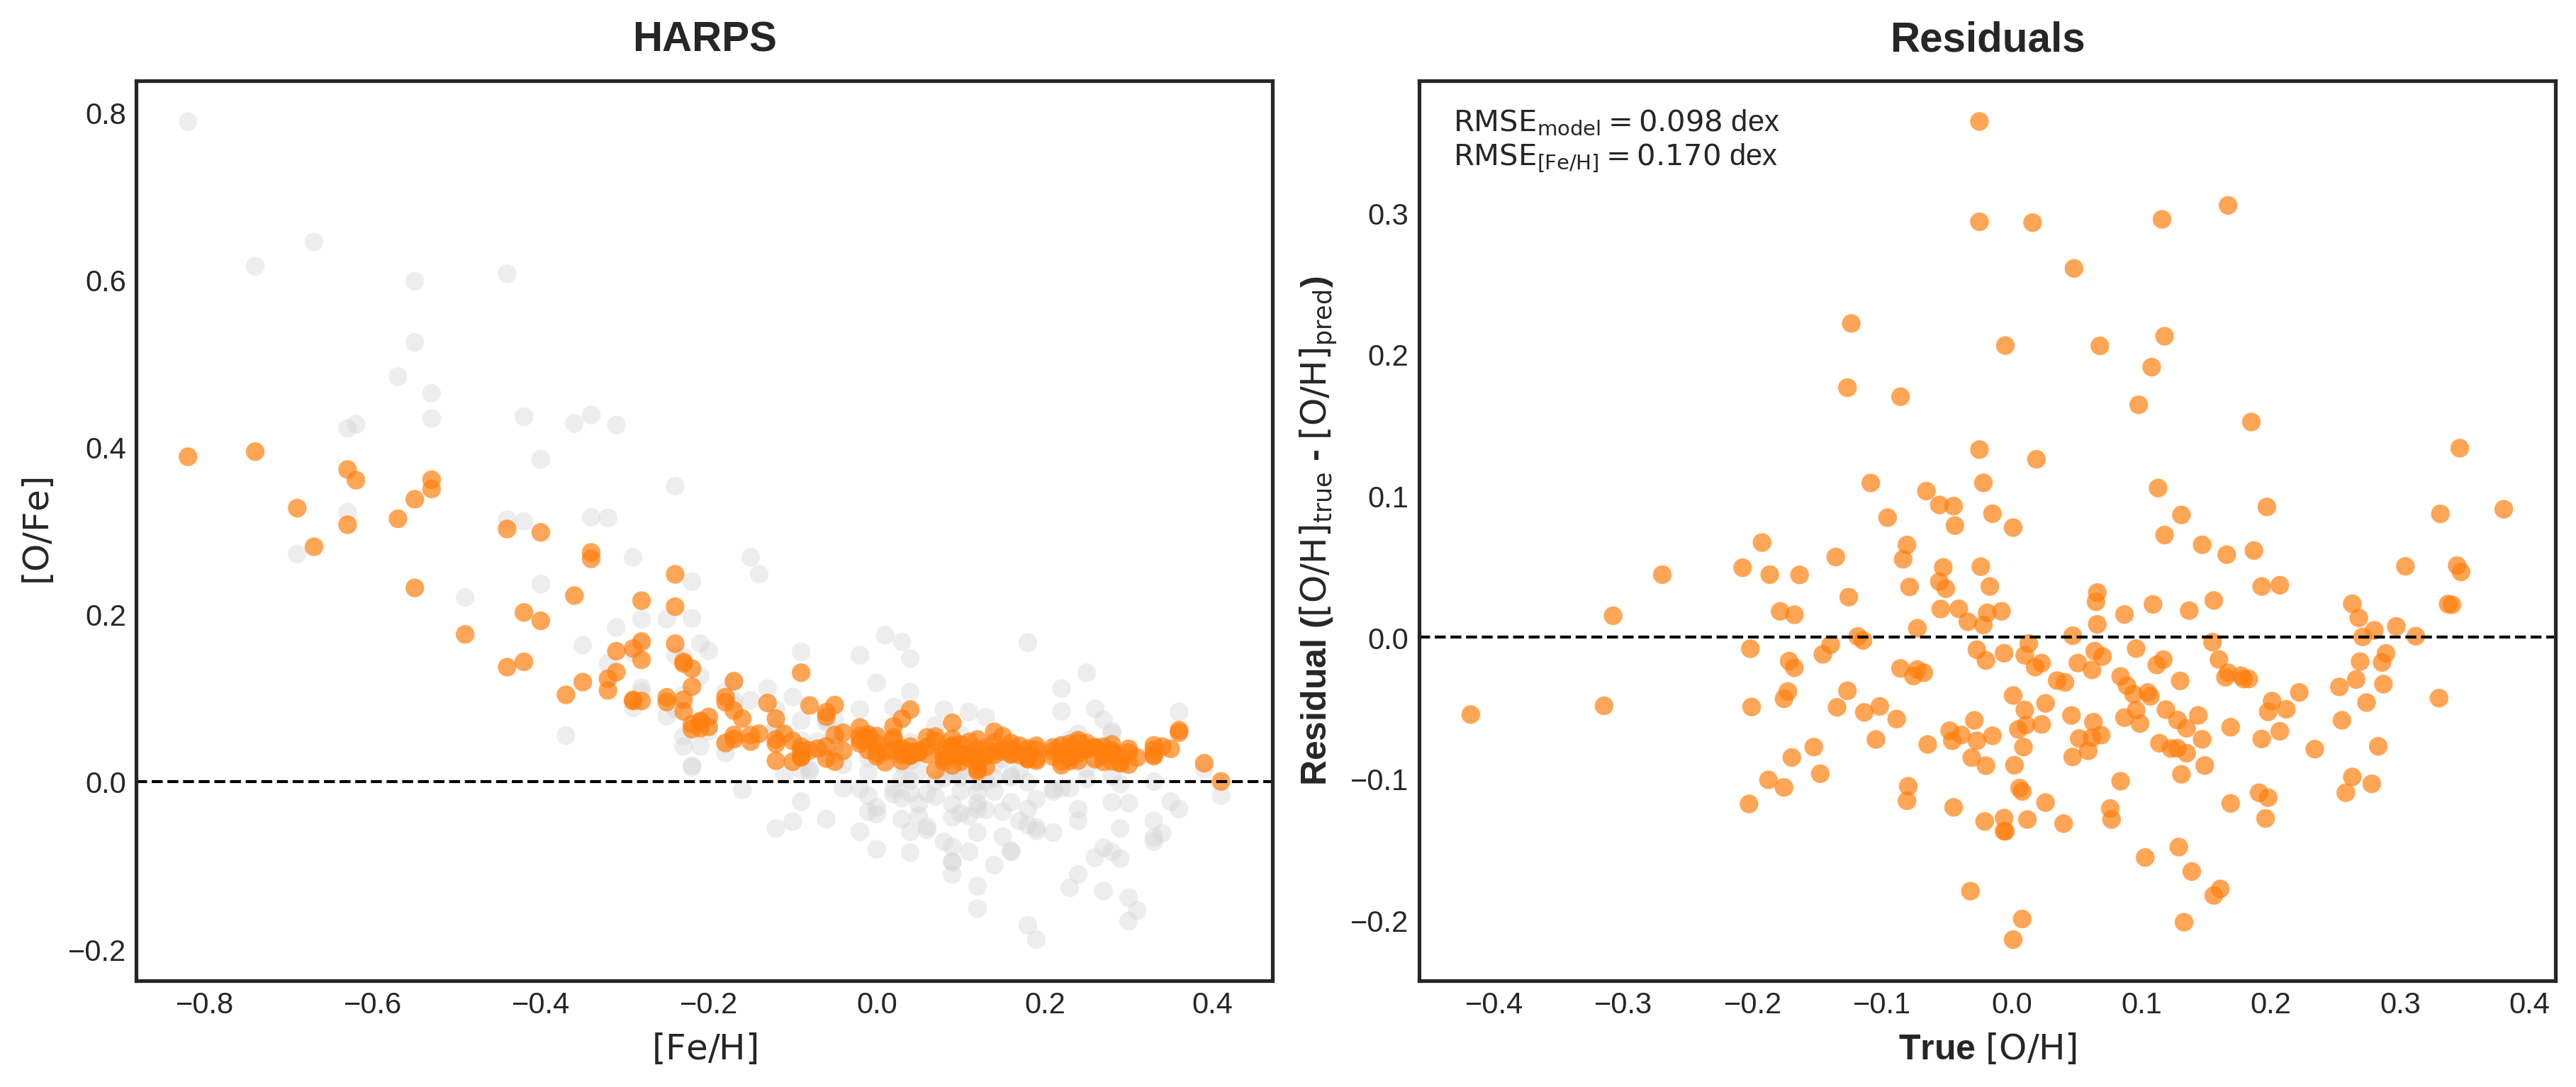
\includegraphics[width=0.48\textwidth]{figures/o_h_harps.png}
\hfill
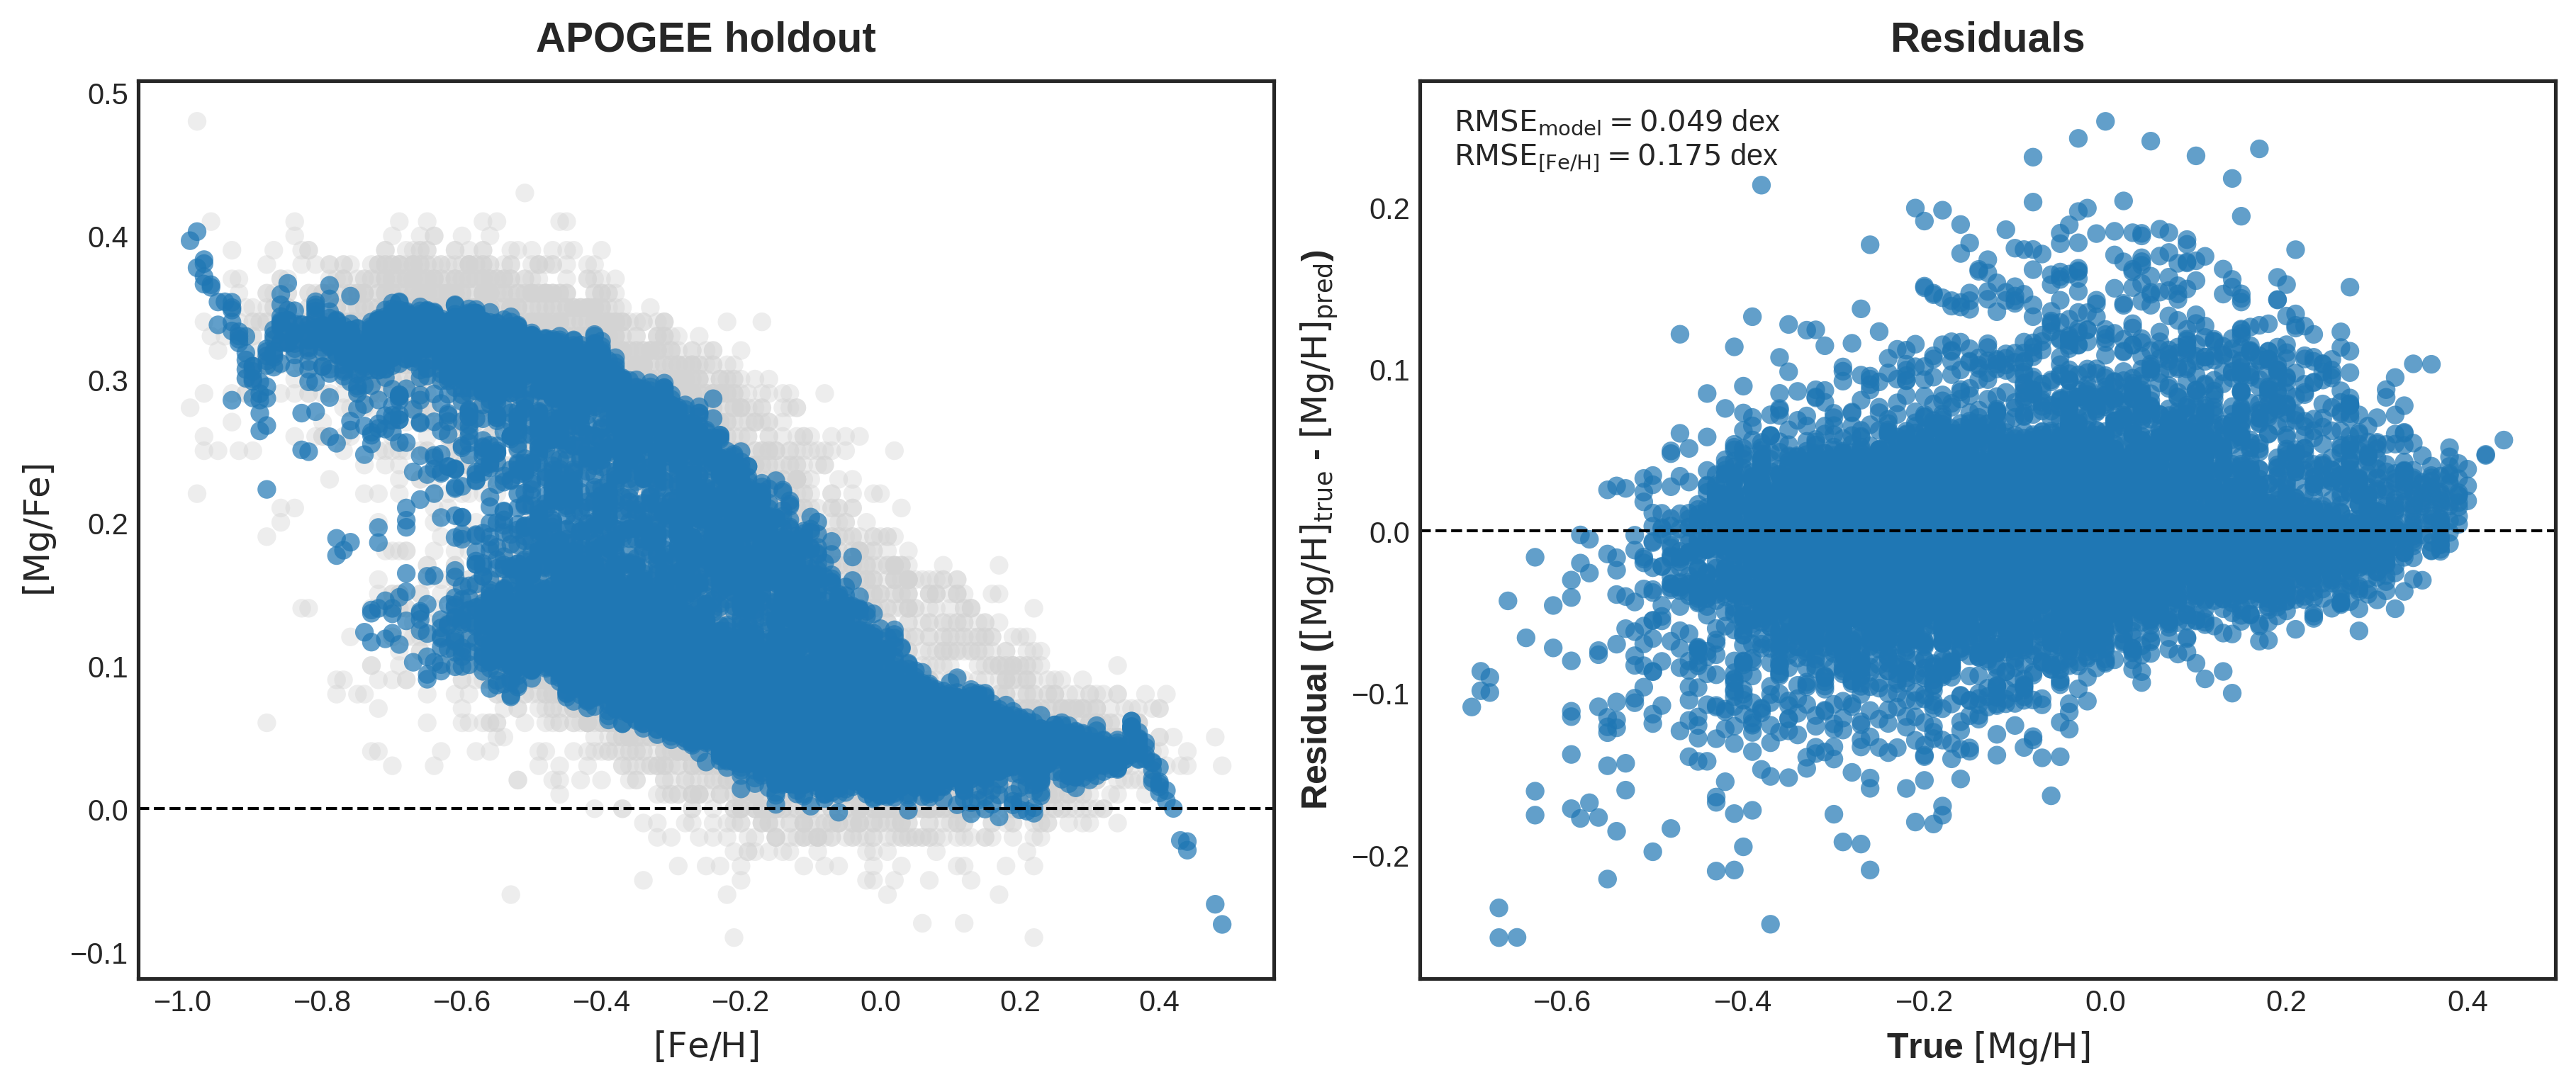
\includegraphics[width=0.48\textwidth]{figures/mg_h_apogee_holdout.png}
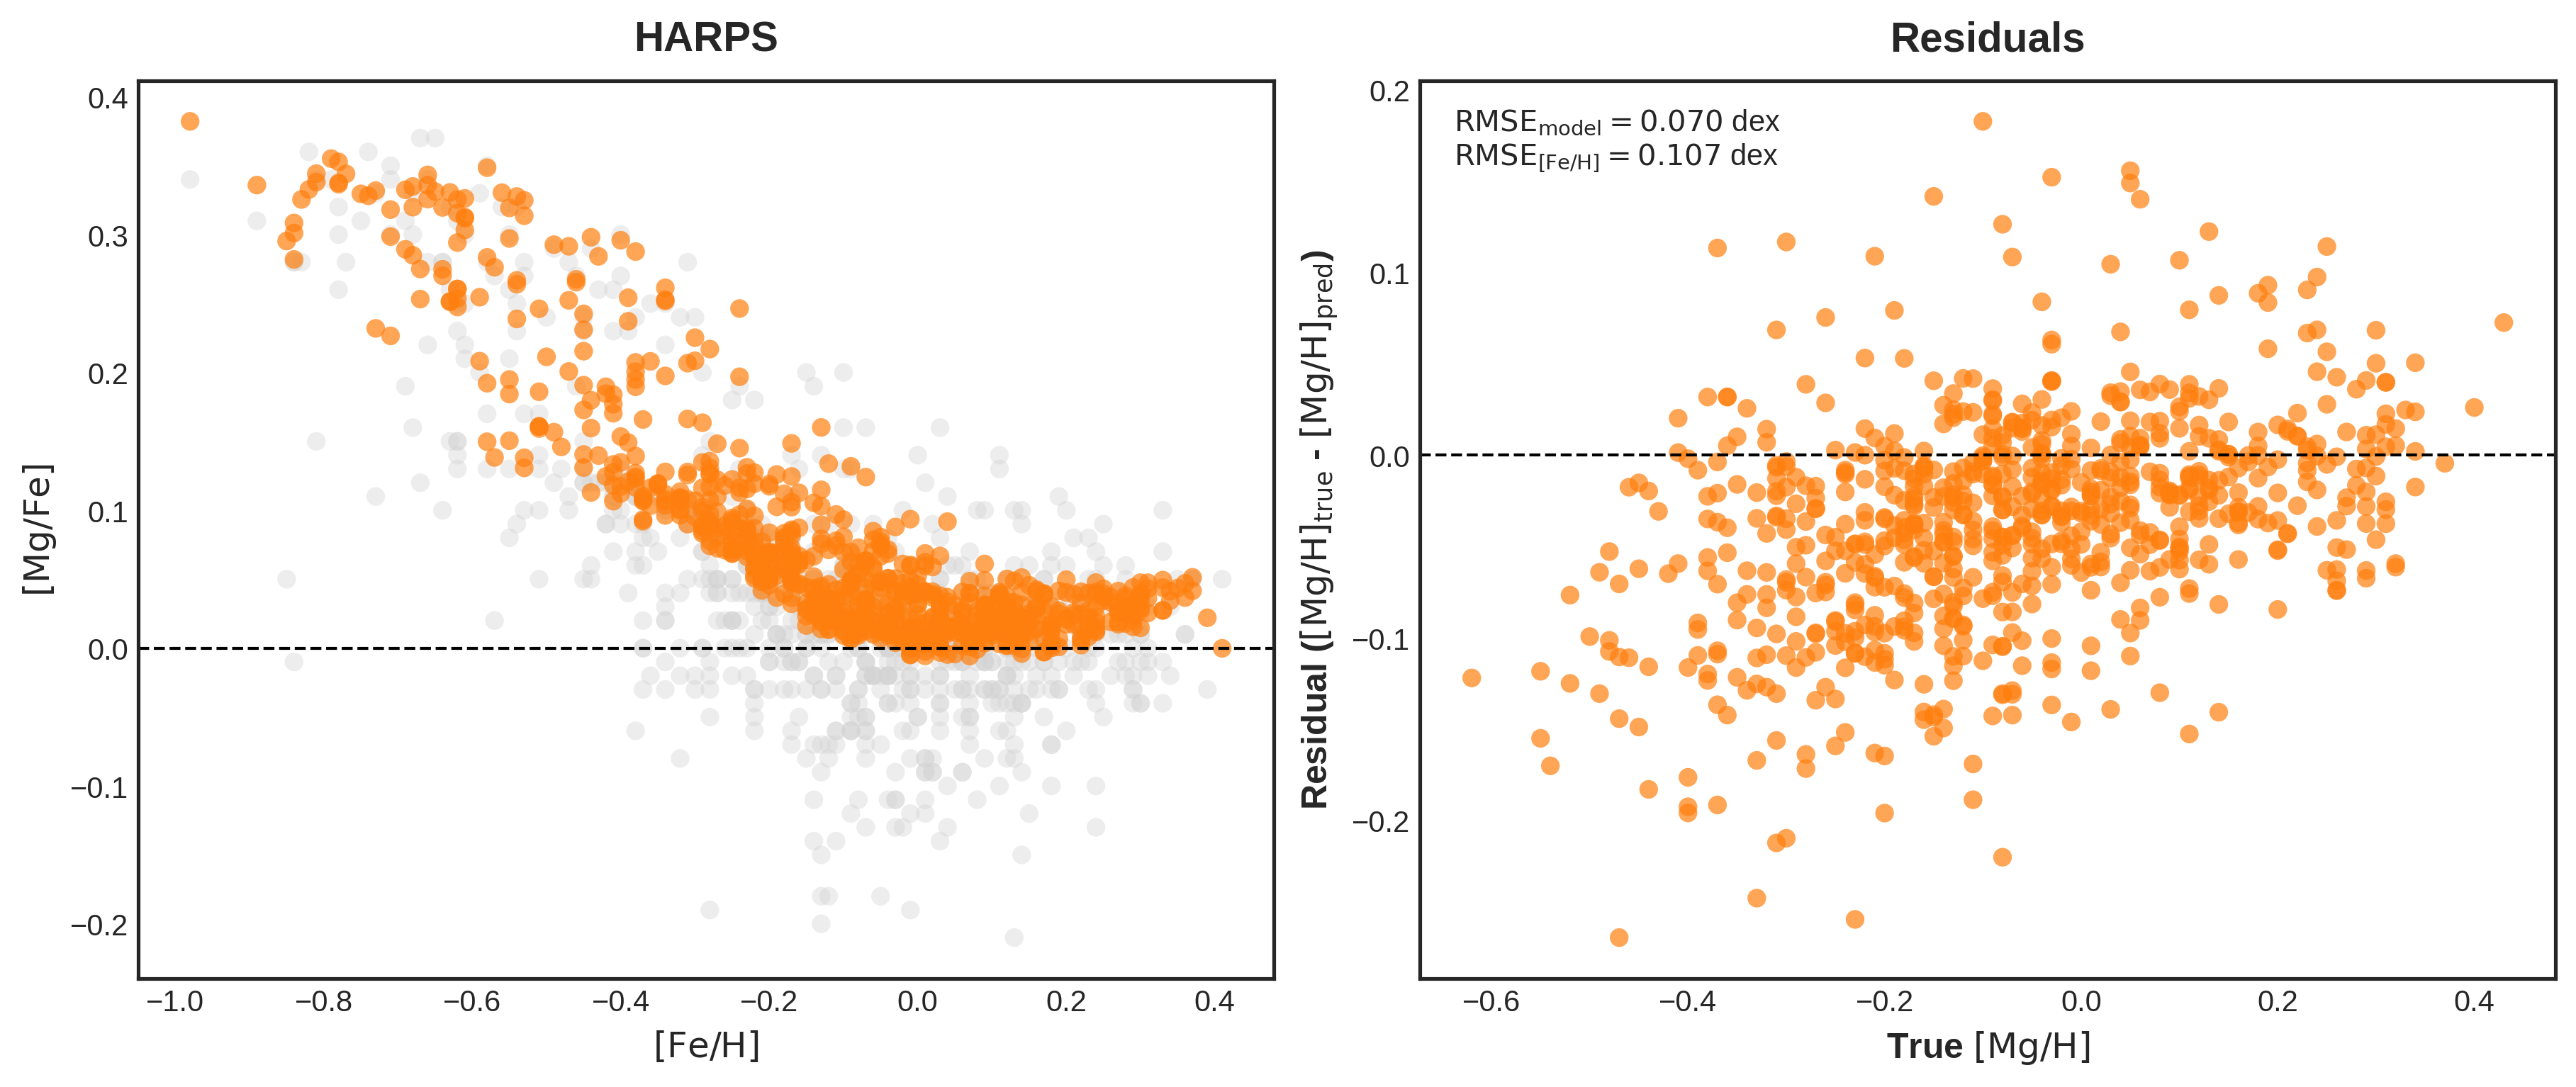
\includegraphics[width=0.48\textwidth]{figures/mg_h_harps.png}
\hfill
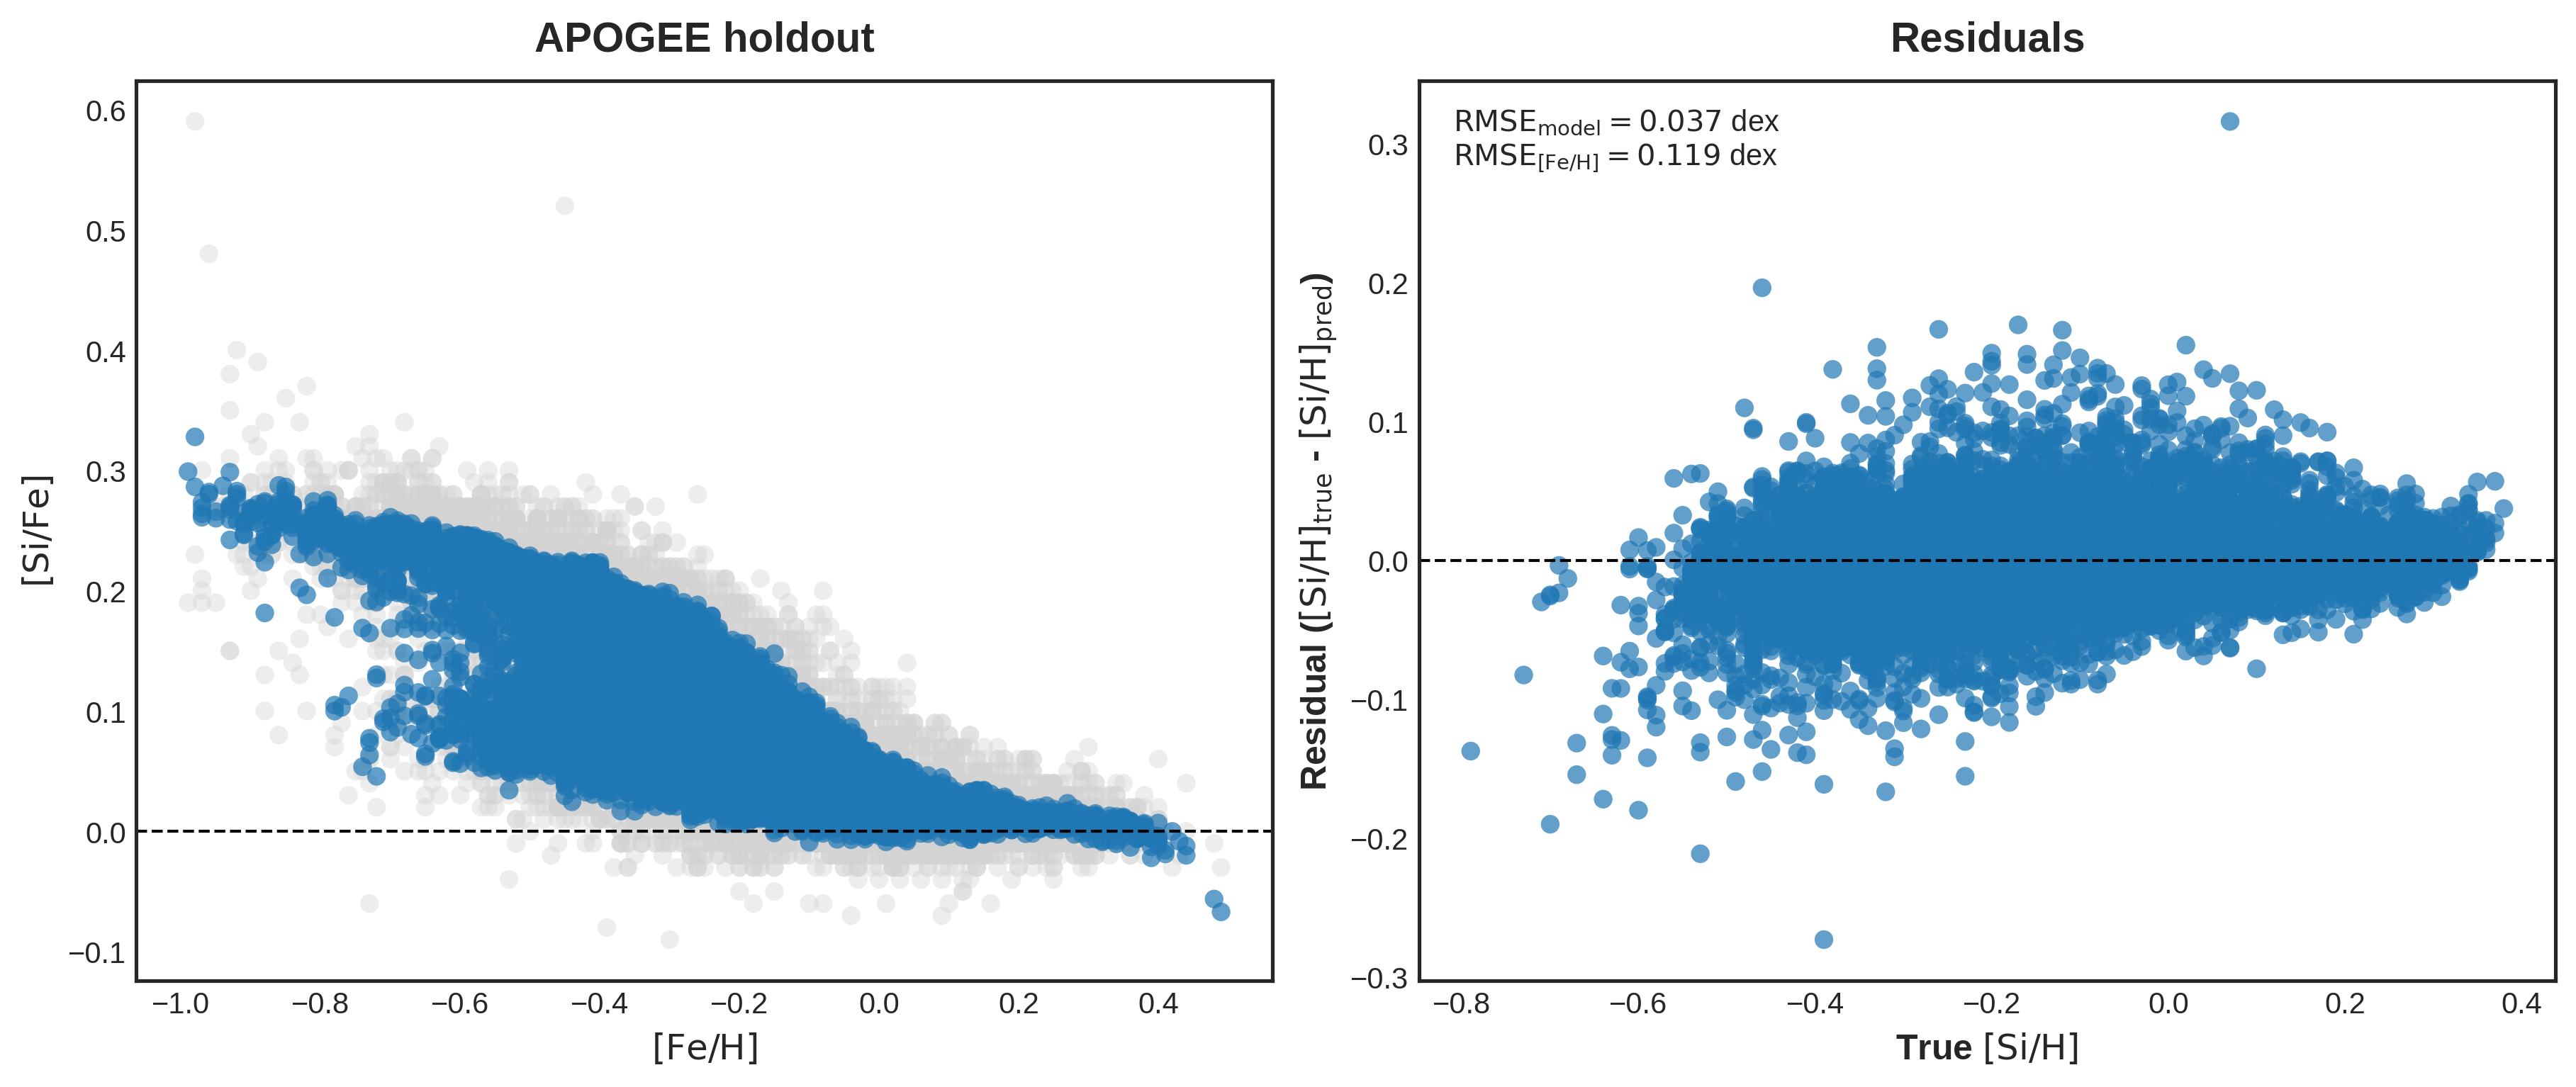
\includegraphics[width=0.48\textwidth]{figures/si_h_apogee_holdout.png}
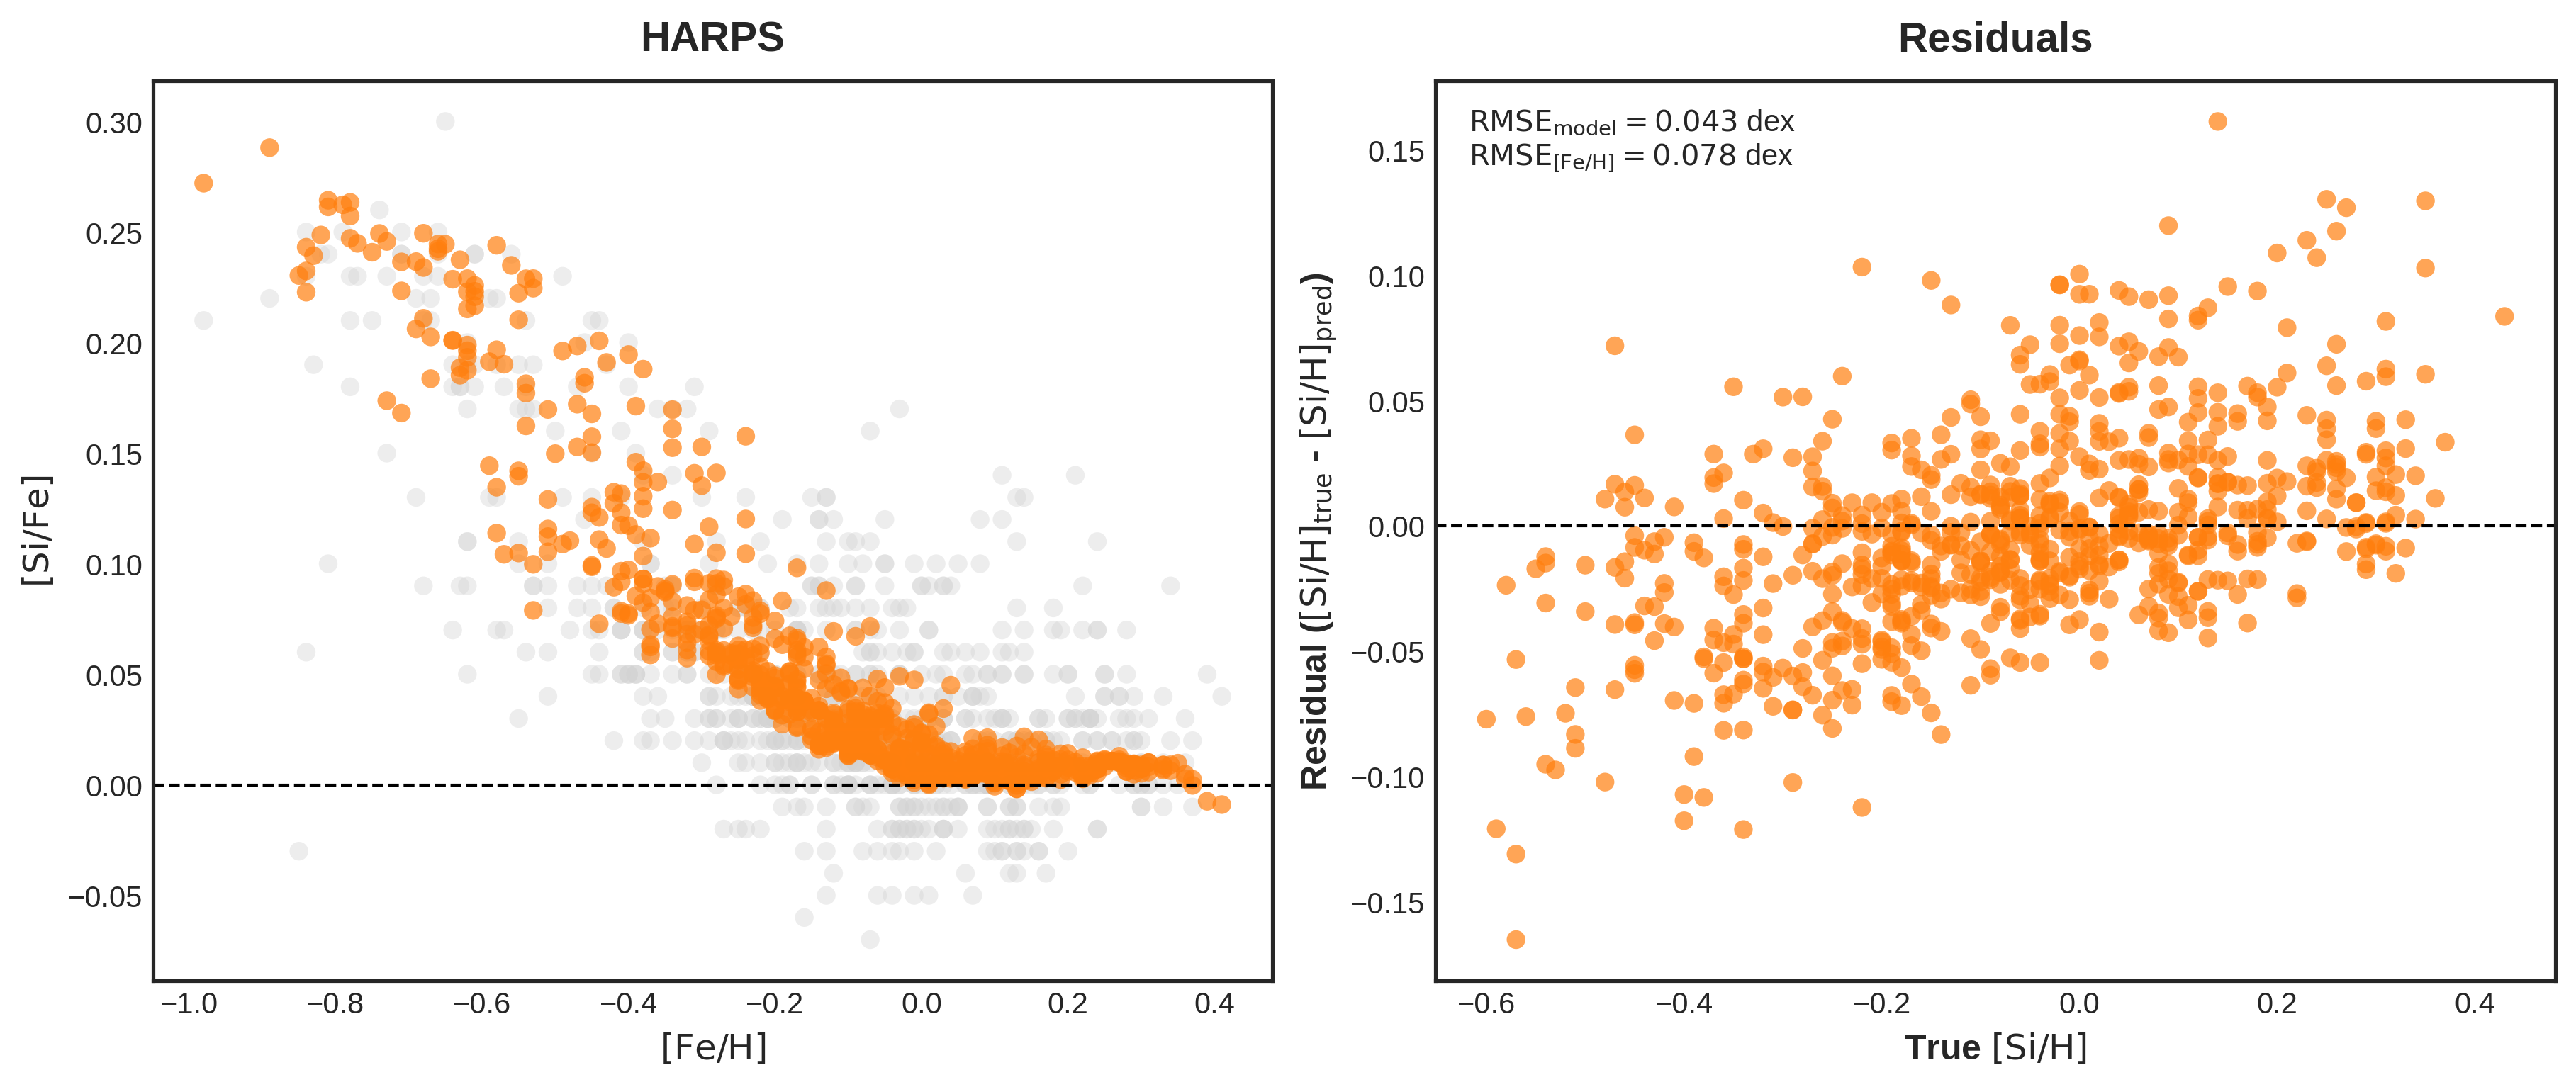
\includegraphics[width=0.48\textwidth]{figures/si_h_harps.png}
\caption{
Predictions of elemental abundances using the tuned LightGBM models.
For each element the left panels show the predicted abundance ratios as a function of metallicity for the APOGEE holdout sample, while the right panels correspond to predictions for the independent HARPS dataset. Grey points indicate the true stellar abundances and coloured points show the model predictions. The accompanying panels display the residuals between true and predicted abundances as a function of the true abundance.}
\label{fig:abundance_predictions}
\end{figure*}



\subsection{Feature importance analysis}
\label{main_feat_imp_abund_feh}

As in the metallicity analysis (Sect.~\ref{feh_from_kinematics}), we examined the relative importance of the input parameters when predicting individual abundances from stellar metallicity and kinematic properties. We used the same four complementary diagnostics: built-in gain importance from the LightGBM model, permutation importance, predictive performance of single-feature models, and global SHAP importance. The full set of figures is presented in Appendix~\ref{appendix:feature_importance_abundances_feh}.

As expected, stellar metallicity [Fe/H] emerges as the dominant predictor for all considered elements. This reflects the strong chemical coupling between the abundances of C, O, Mg, and Si and the overall metallicity driven by Galactic chemical evolution. Across all importance diagnostics, [Fe/H] consistently exhibits the largest contribution to the model predictions.

Among the remaining parameters, the orbital pericentric distance $R_{\mathrm{peri}}$ typically provides the next most significant contribution, while  $Z_{\max}$ has a smaller but still measurable impact. The remaining kinematic parameters contribute only marginally once metallicity and the main orbital parameters are included.


To further explore the role of stellar metallicity in the abundance predictions, we examined SHAP dependence plots for [Fe/H] in the tuned LightGBM models (Fig.~\ref{fig:shap_dependence_abundances_feh}). The SHAP values show an almost perfectly monotonic relation with [Fe/H] for all considered elements (C, O, Mg, and Si).

The colour-coding by the pericentric orbital distance $R_{\mathrm{peri}}$ reveals a secondary modulation of the predictions. At metallicities above approximately $[\mathrm{Fe/H}] \gtrsim -0.1$ dex, stars with larger $R_{\mathrm{peri}}$ tend to exhibit slightly higher SHAP contributions, indicating somewhat enhanced predicted abundances relative to stars with smaller pericentric distances. At lower metallicities the trend appears to reverse. Although this effect is subtle compared to the dominant metallicity dependence, it suggests that orbital properties encode additional information related to population mixing and Galactic chemical history that is not fully captured by [Fe/H] alone.

We performed the same analysis using $Z_{\max}$ instead of $R_{\mathrm{peri}}$, but no clear dependence of the SHAP values on $Z_{\max}$ was visually apparent in the corresponding dependence plots.

\begin{figure*}[ht]
\centering
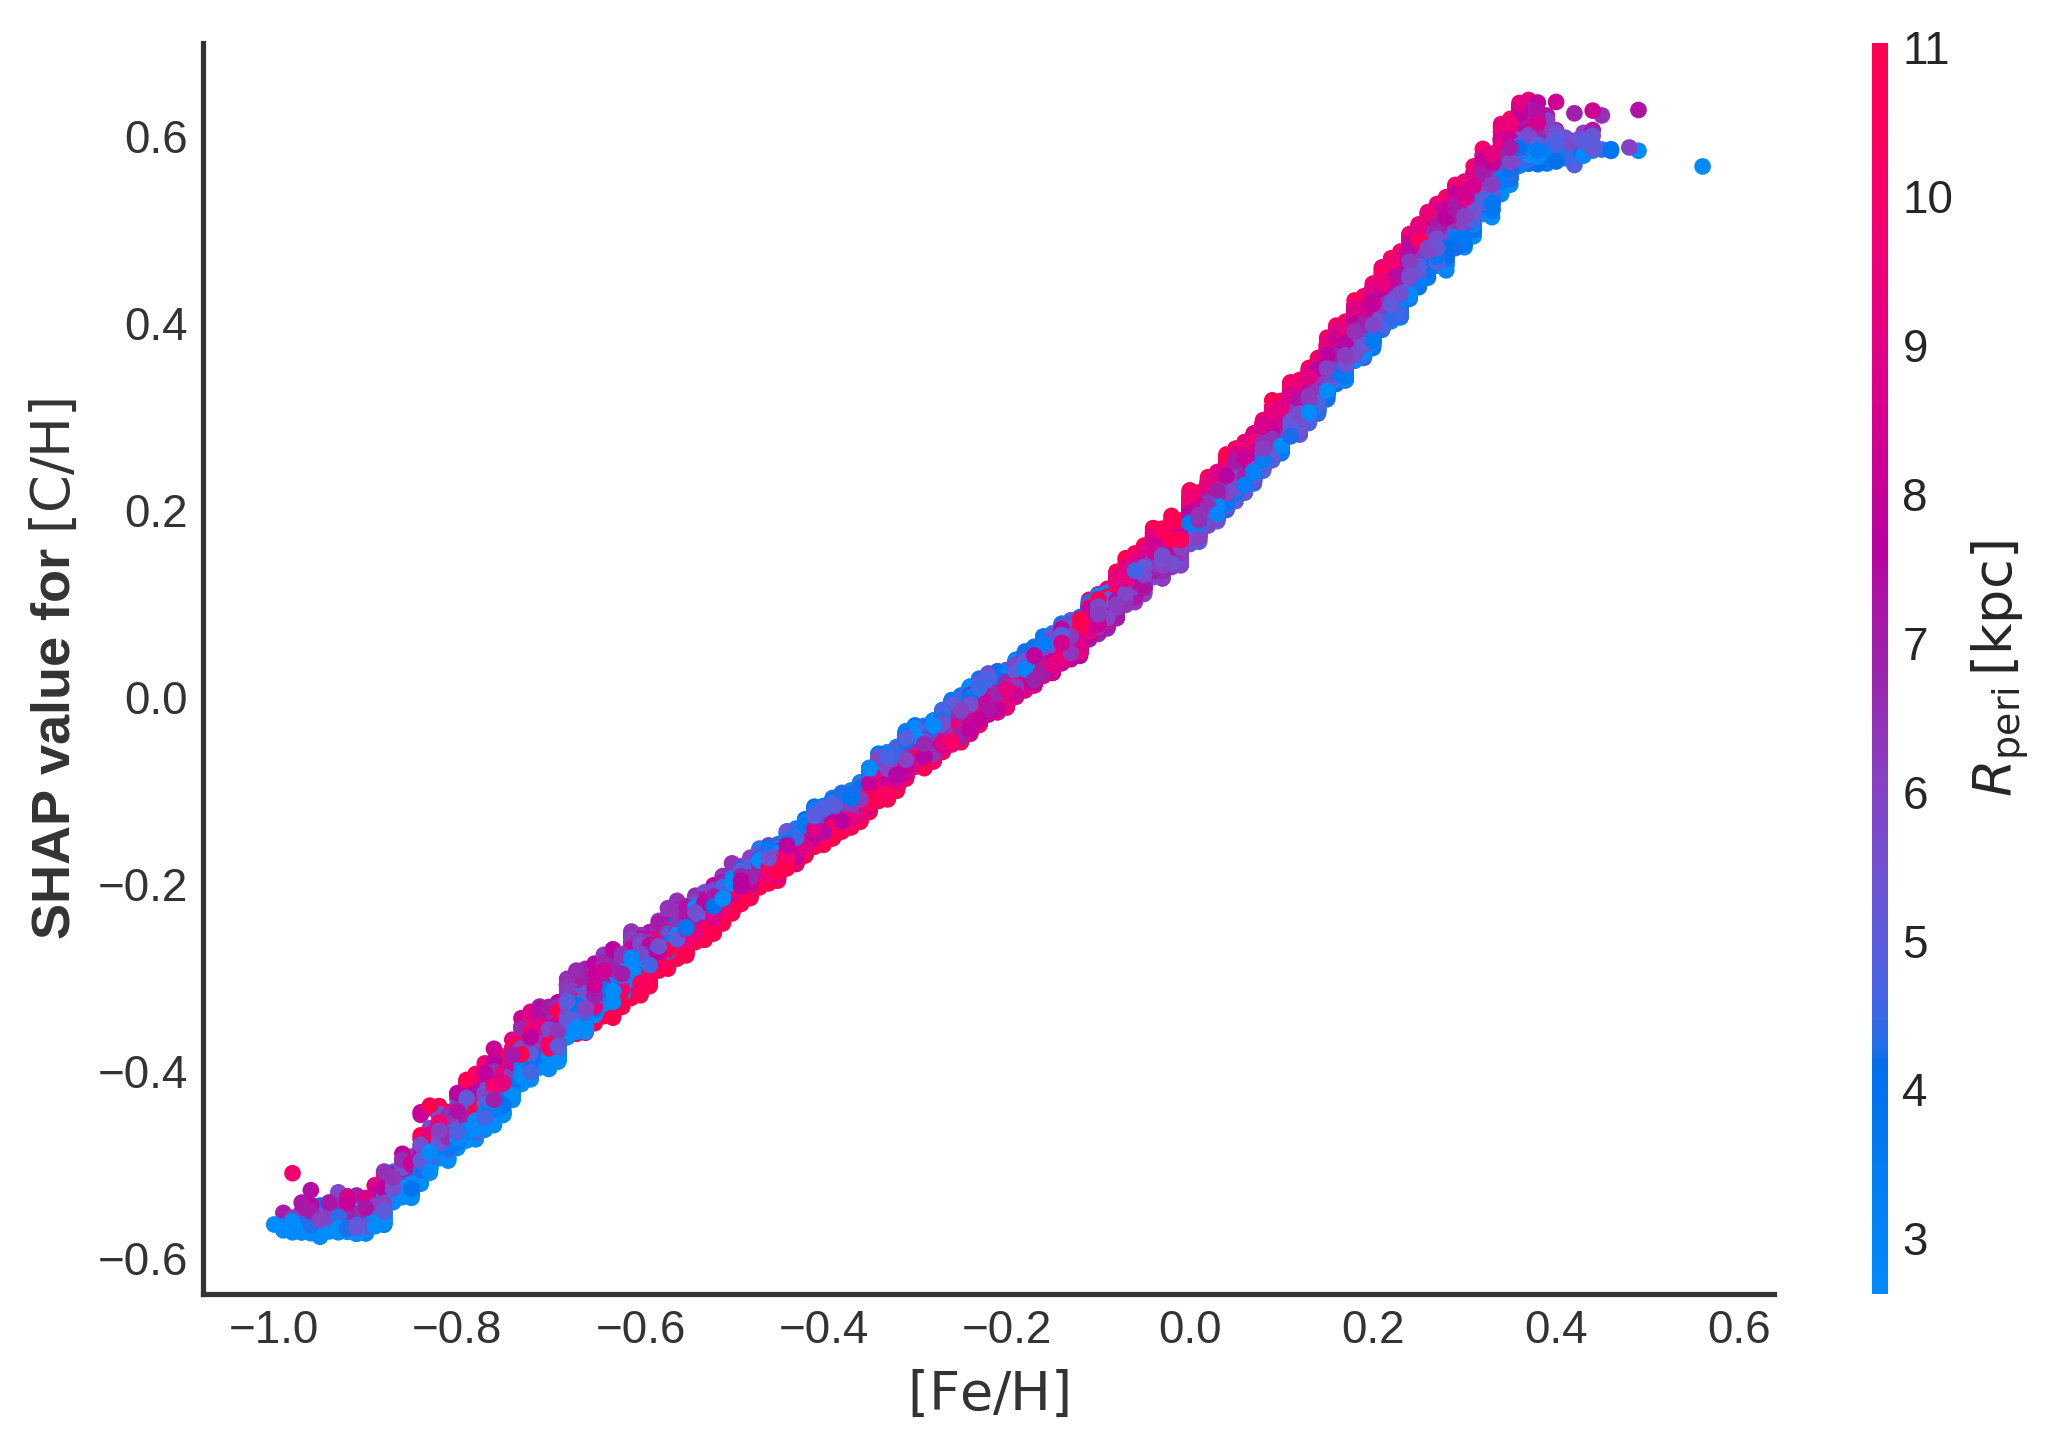
\includegraphics[width=0.4\textwidth]{figures/LGBM_c_h_dependence_fe_h_by_rperi.png}
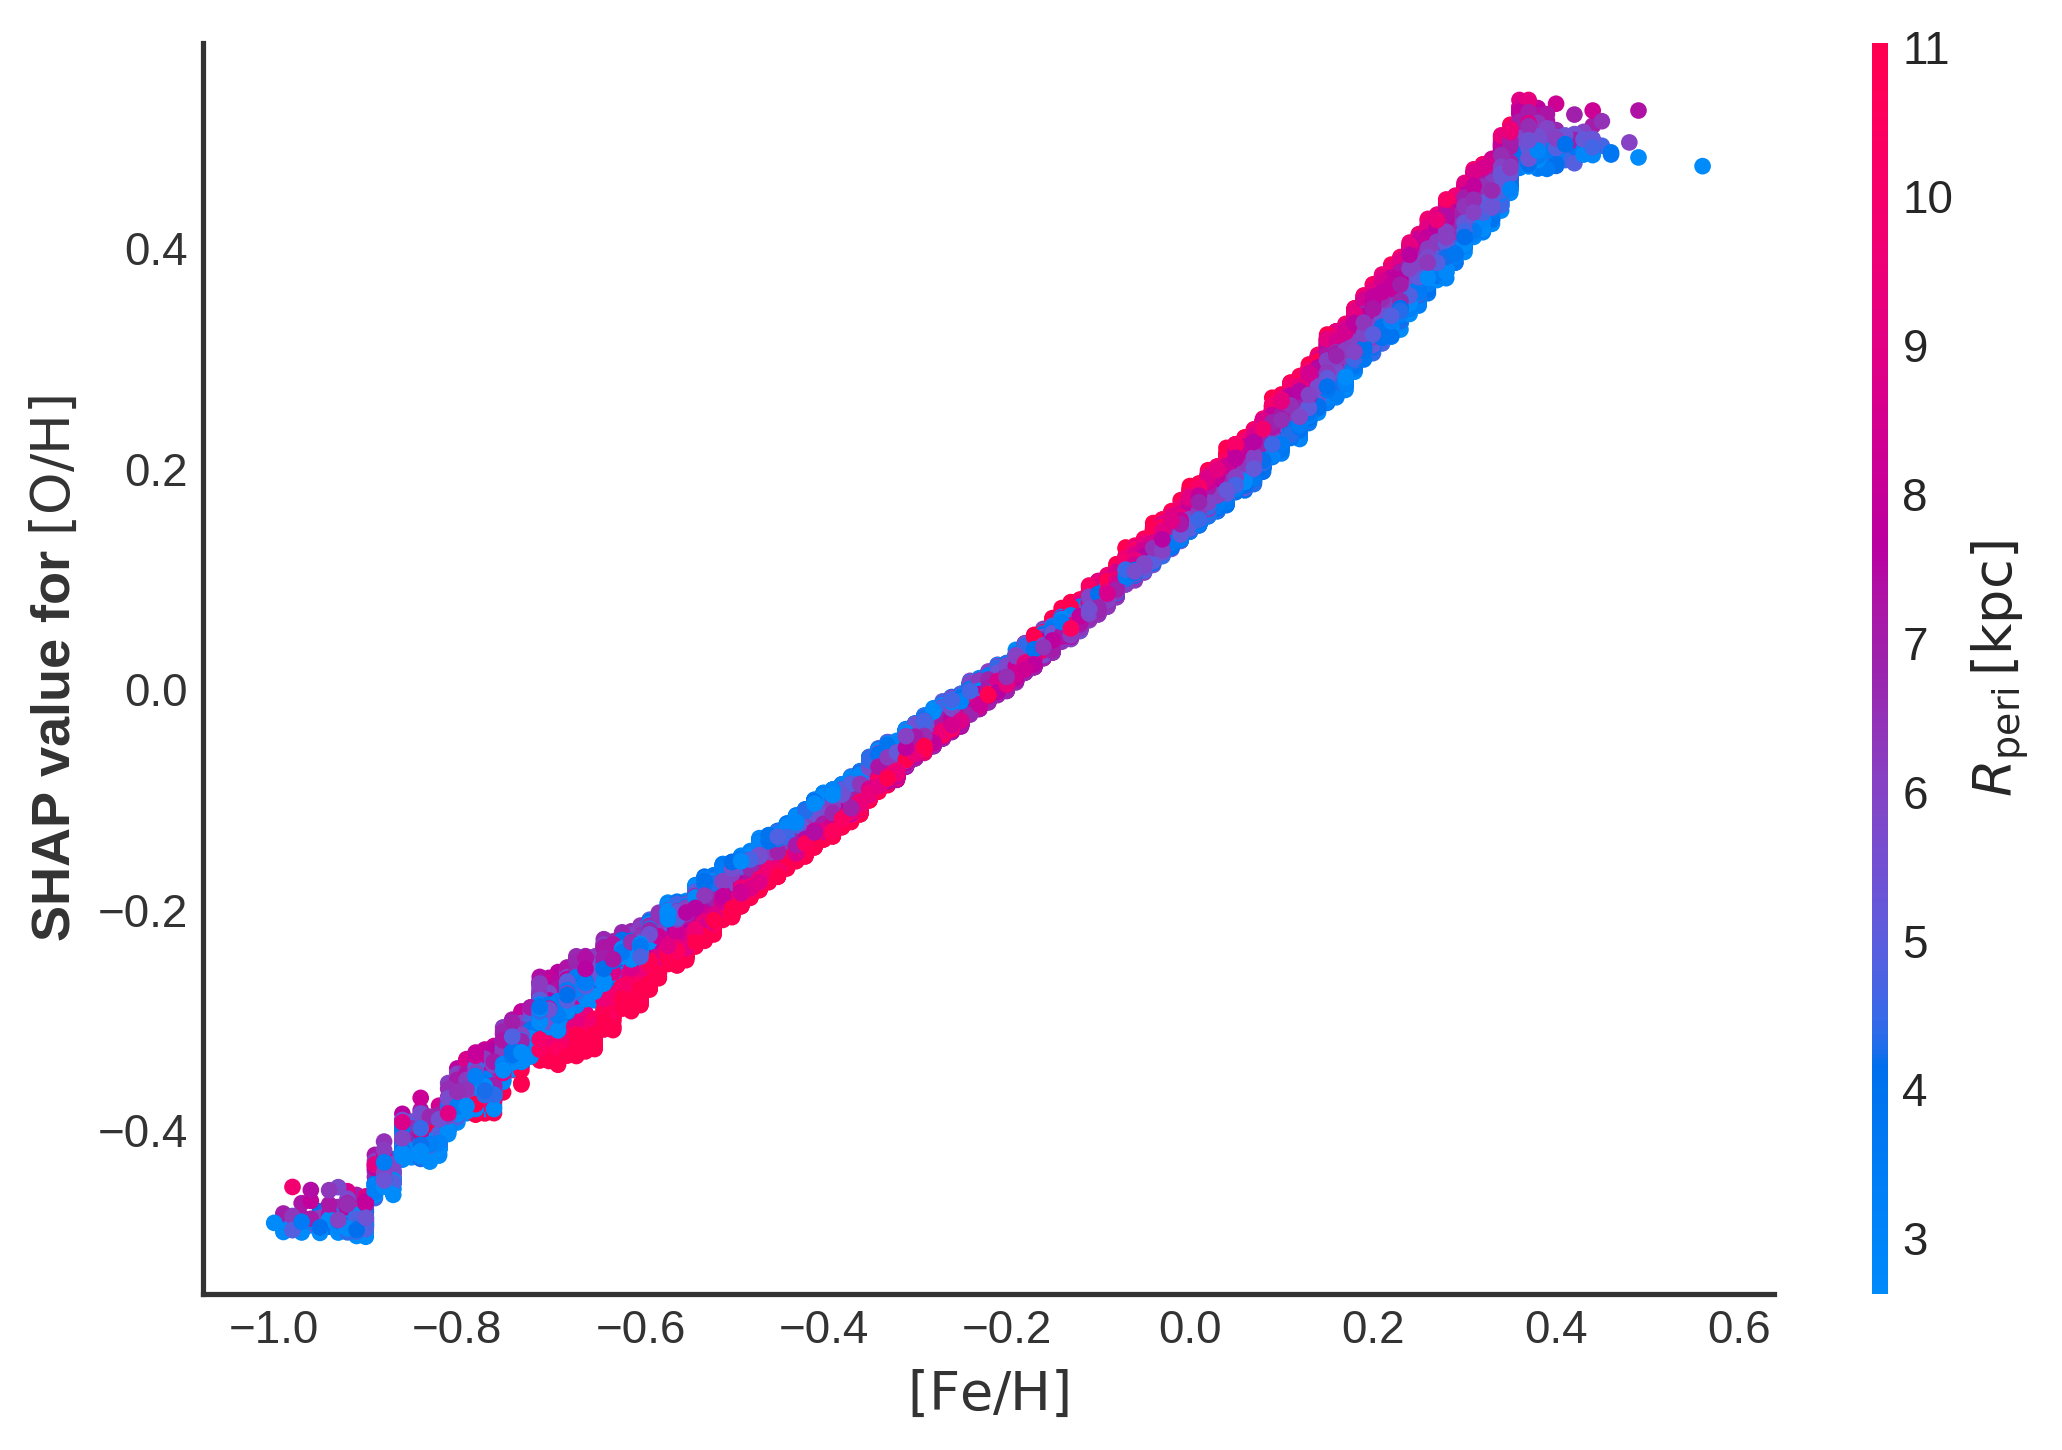
\includegraphics[width=0.4\textwidth]{figures/LGBM_o_h_dependence_fe_h_by_rperi.png}
\vspace{0.4cm}
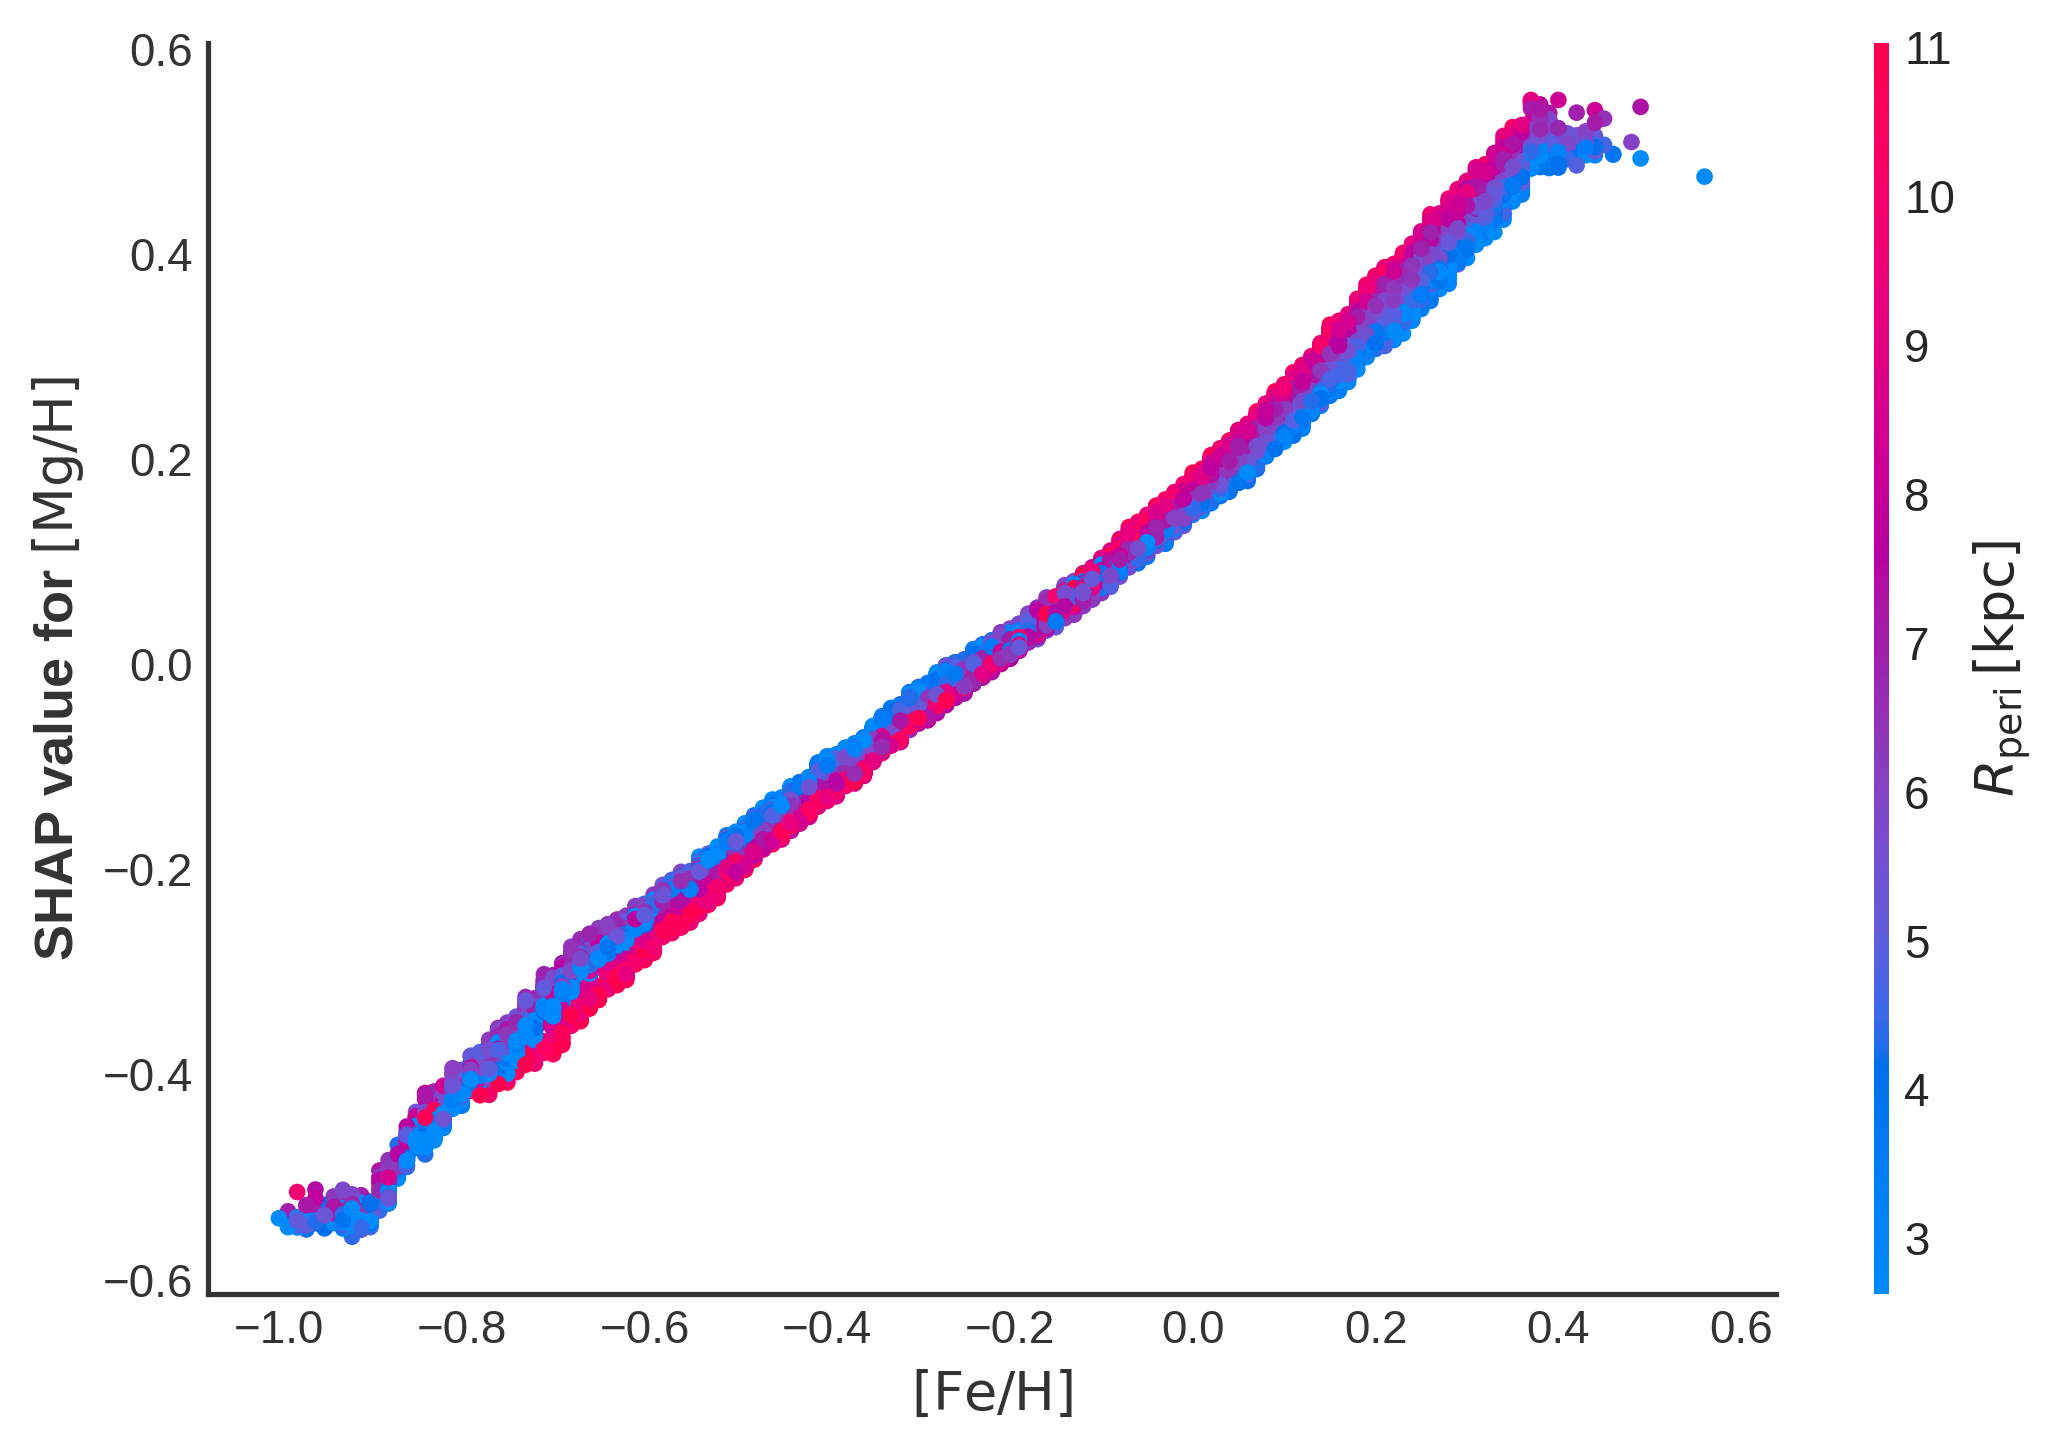
\includegraphics[width=0.4\textwidth]{figures/LGBM_mg_h_dependence_fe_h_by_rperi.png}
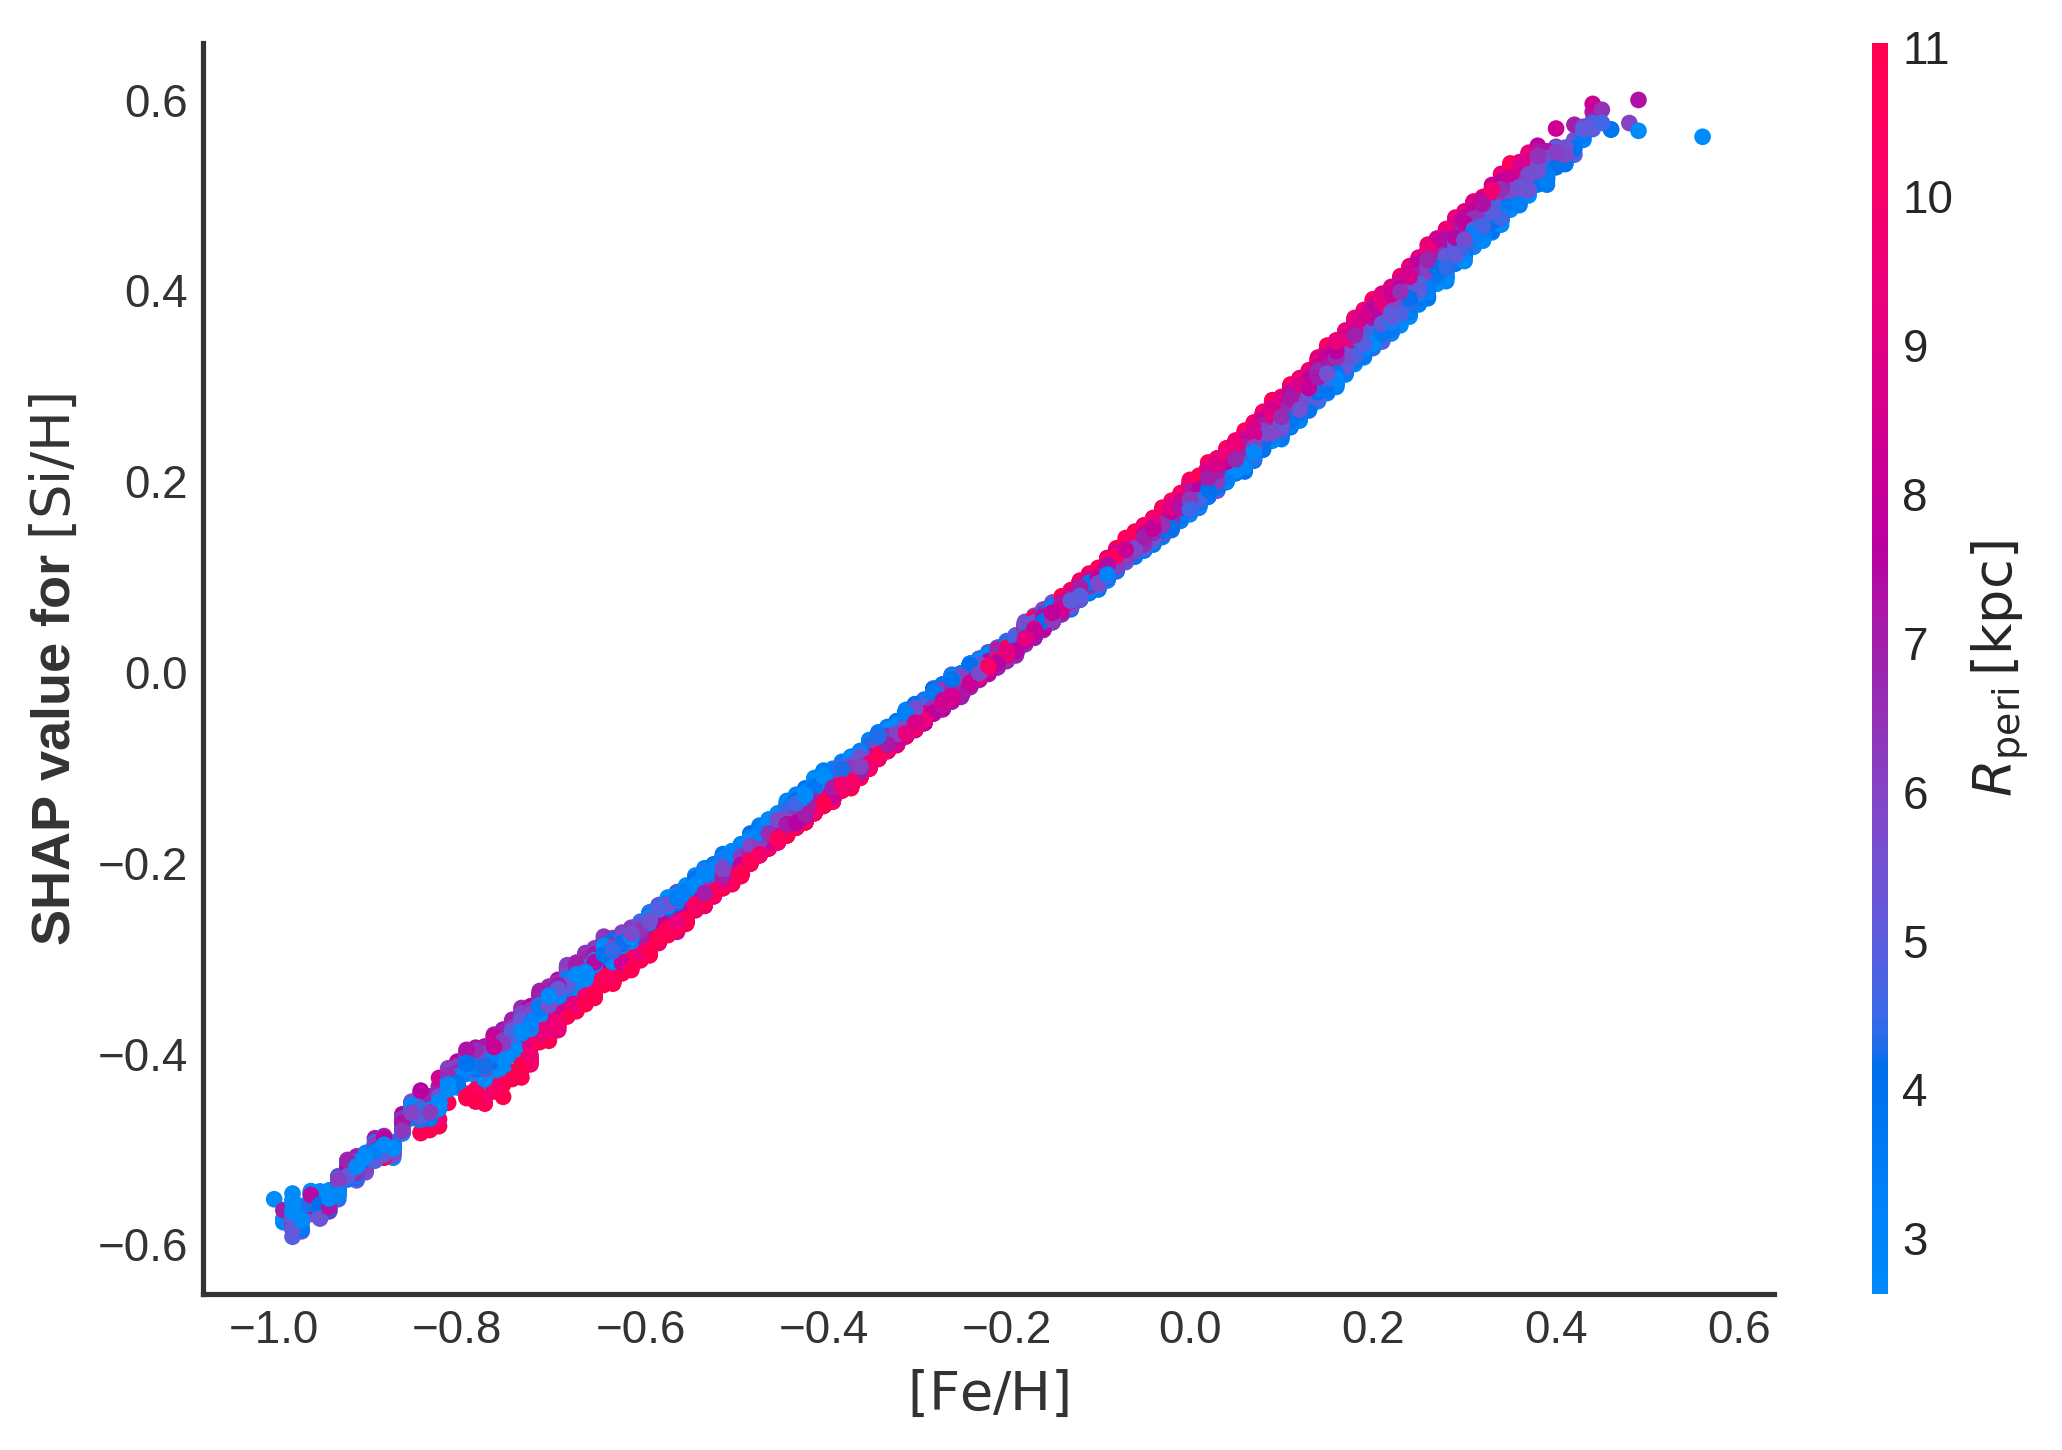
\includegraphics[width=0.4\textwidth]{figures/LGBM_si_h_dependence_fe_h_by_rperi.png}
\caption{SHAP dependence plots showing the contribution of stellar metallicity [Fe/H] to the predicted abundances of individual elements using the tuned LightGBM models. From top left to bottom right the panels correspond to [C/H], [O/H], [Mg/H], and [Si/H]. The vertical axis shows the SHAP value associated with [Fe/H], while the horizontal axis shows the stellar metallicity itself. Points are colour-coded by  $R_{\mathrm{peri}}$.}
\label{fig:shap_dependence_abundances_feh}
\end{figure*}


\section{Predicting C and O abundances from Mg, Si, and Fe}
\label{main_CO_from_MgSiFe}

In this section, we predict the abundances of carbon and oxygen from the abundances of Mg, Si, and [Fe/H], optionally complemented by kinematic and orbital parameters. This is particularly relevant for relatively cool stars, for which the determination of C and O abundances is challenging.

Following the same methodology adopted in the previous sections, we benchmarked a range of regression algorithms. Consistent with the previous results, LightGBM yields the lowest RMSE and is therefore adopted as the reference model.

Baseline models trained using only Mg, Si, and [Fe/H] already achieve strong predictive performance. The inclusion of additional kinematic and orbital parameters does not lead to a measurable improvement in RMSE, indicating that most of the predictive information is already encoded in the elemental abundances themselves.

We also explored a range of feature-engineering strategies aimed at capturing nonlinear interactions between the input abundances. These included combinations such as the mean abundance of Mg and Si, as well as pairwise differences (e.g., Mg$-$Si, Mg$-$Fe, Si$-$Fe) and simple algebraic transformations. However, none of these engineered features produced a measurable improvement in predictive accuracy.

For both C and O abundance predictions, we find that Mg abundance carries the dominant predictive power. In fact, models trained using only Mg abundance achieve RMSE values comparable to those obtained when including Si and [Fe/H]. This result indicates a strong coupling between Mg and the C and O abundances, reflecting their common nucleosynthetic origin. The feature-importance analysis is presented in Appendix~\ref{appendix:CO_from_MgSiFe}, where we show the results of gain-based importance, permutation importance, SHAP values, and single-feature predictive performance.

Figure~\ref{fig:CO_predictions} illustrates the performance of the tuned LightGBM models for predicting [O/H] and [C/H] using the APOGEE holdout sample and the independent HARPS dataset. The left panels show the predicted abundance ratios as a function of metallicity, while the right panels display the residuals as a function of the true abundance.

For the APOGEE sample, the model reproduces the global abundance trends remarkably well, capturing both the overall slope and the intrinsic scatter of the [O/Fe]--[Fe/H] relation. The predicted values closely follow the true abundances across the full metallicity range, although a mild compression of the dynamic range is visible. This behaviour is consistent with the regression-to-the-mean effect, arising from incomplete information in the input features. The residuals exhibit a clear heteroscedastic pattern, with slightly larger scatter at lower abundances and a gradual tightening toward higher metallicities.

When applied to the independent HARPS sample, the model performance degrades. In particular, the [O/Fe] ratio at low metallicities is systematically underestimated relative to the HARPS values. Nevertheless, the achieved RMSE remains lower than that obtained from a simple baseline assuming [O/H] = [Mg/H], indicating that the model retains predictive power beyond this approximation.

The situation is less favourable for carbon. A clear offset is observed between the predicted and HARPS [C/H] abundances, with the model systematically underestimating the HARPS values. In fact, assuming [C/H] = [Mg/H] yields a lower RMSE than the direct model predictions. However, this discrepancy is largely driven by a systematic offset between the APOGEE and HARPS abundance scales. After applying a constant correction of $\sim$0.1 dex to the predicted values, the RMSE decreases significantly to $\sim$0.07 dex. This indicates that the dominant source of the discrepancy is not the model itself, but rather a systematic difference between the two datasets.


\begin{figure*}[ht]
\centering
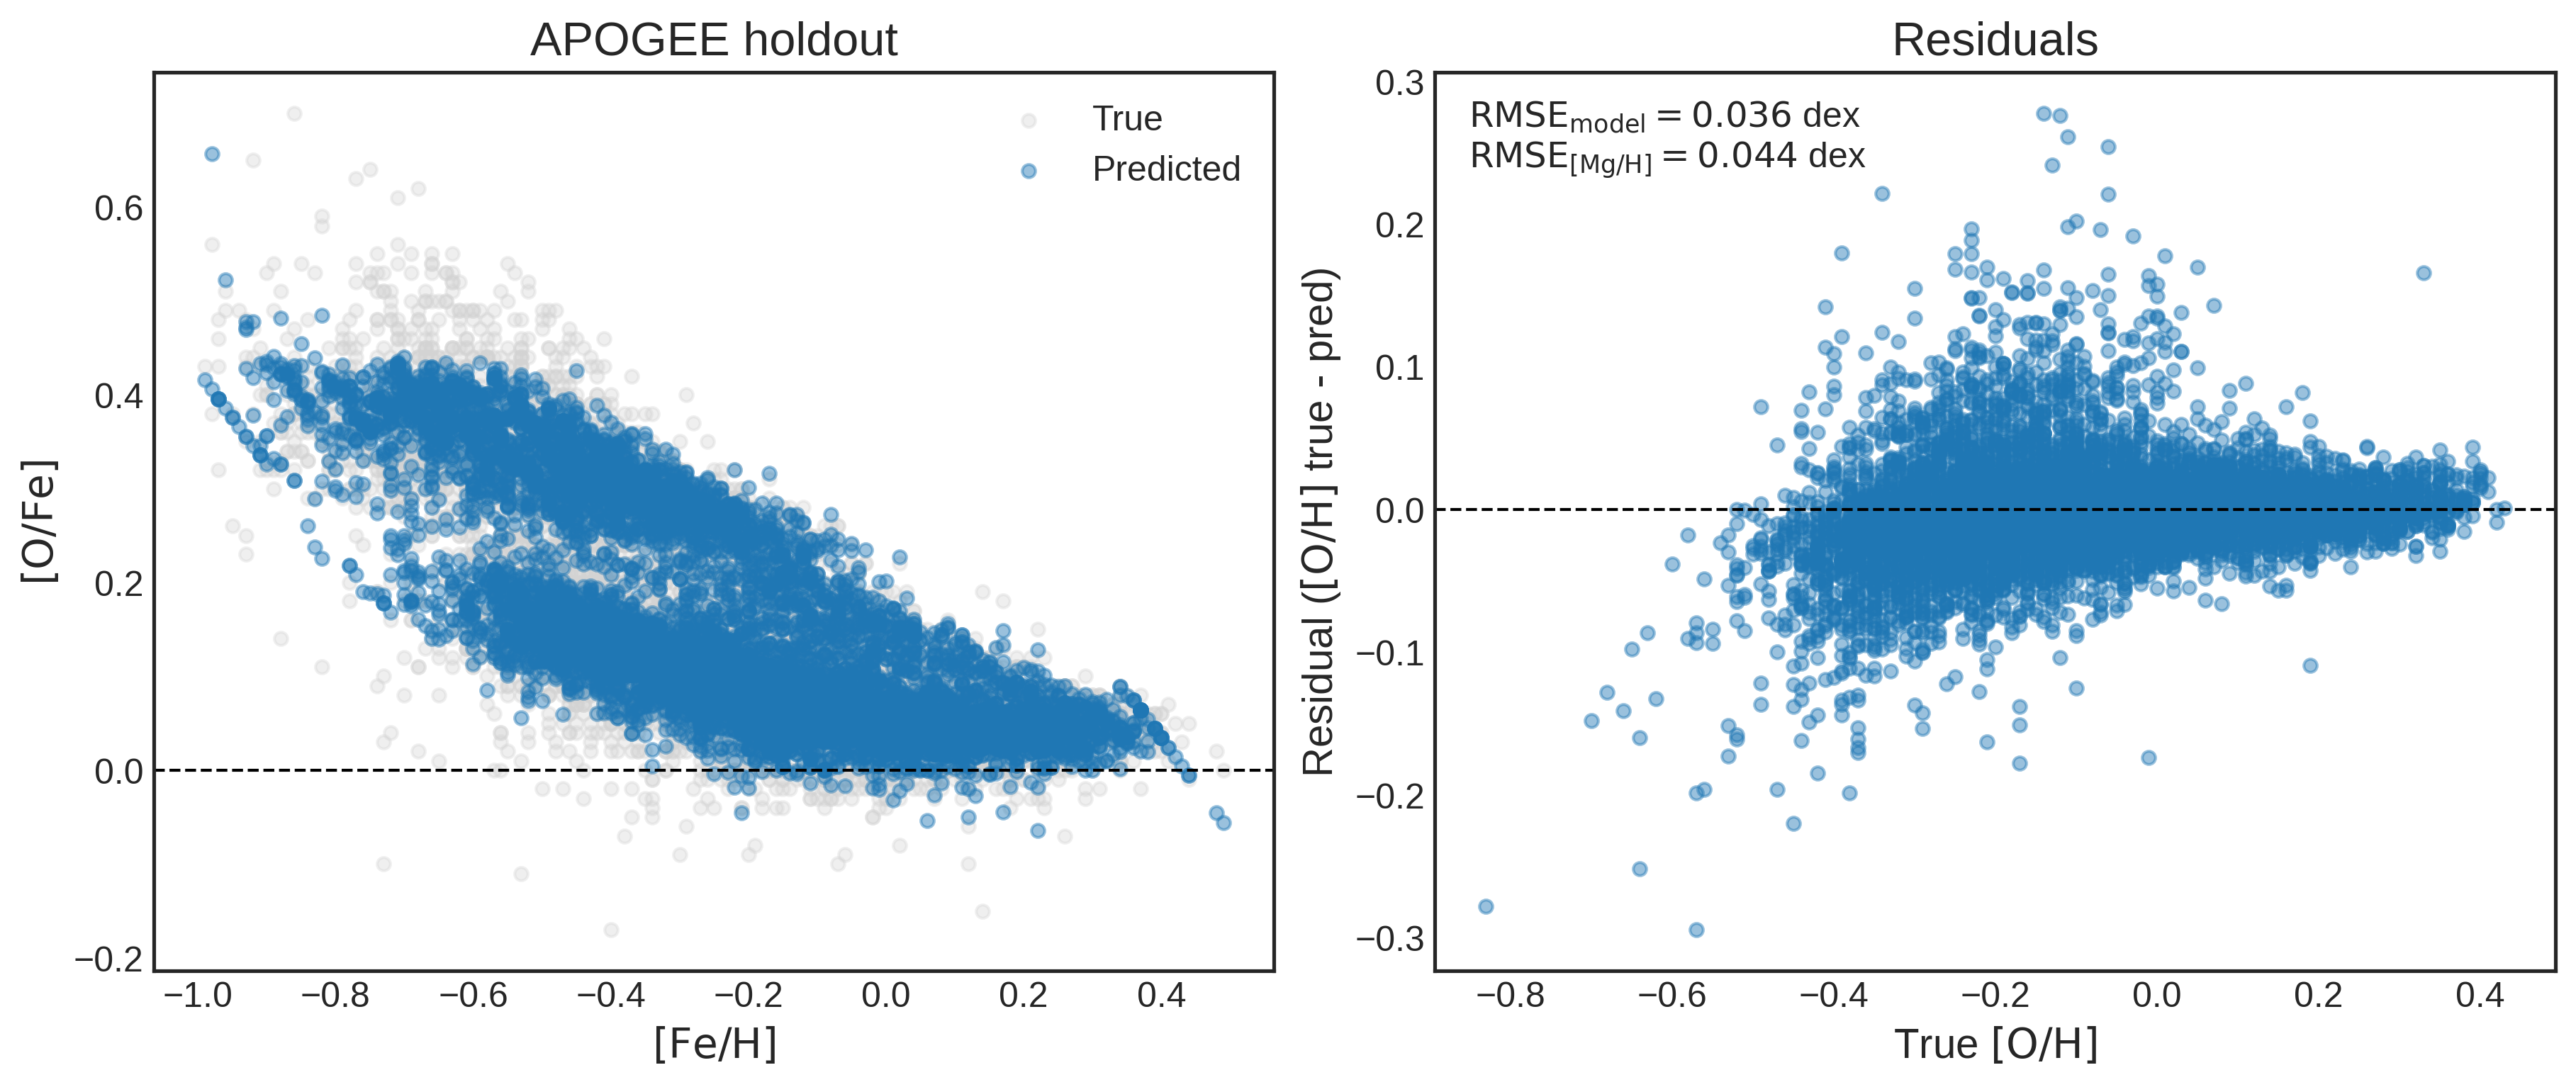
\includegraphics[width=0.48\textwidth]{figures/prediction_panels_apogee_holdout_fe_mg_si_o_h.png}
\hfill
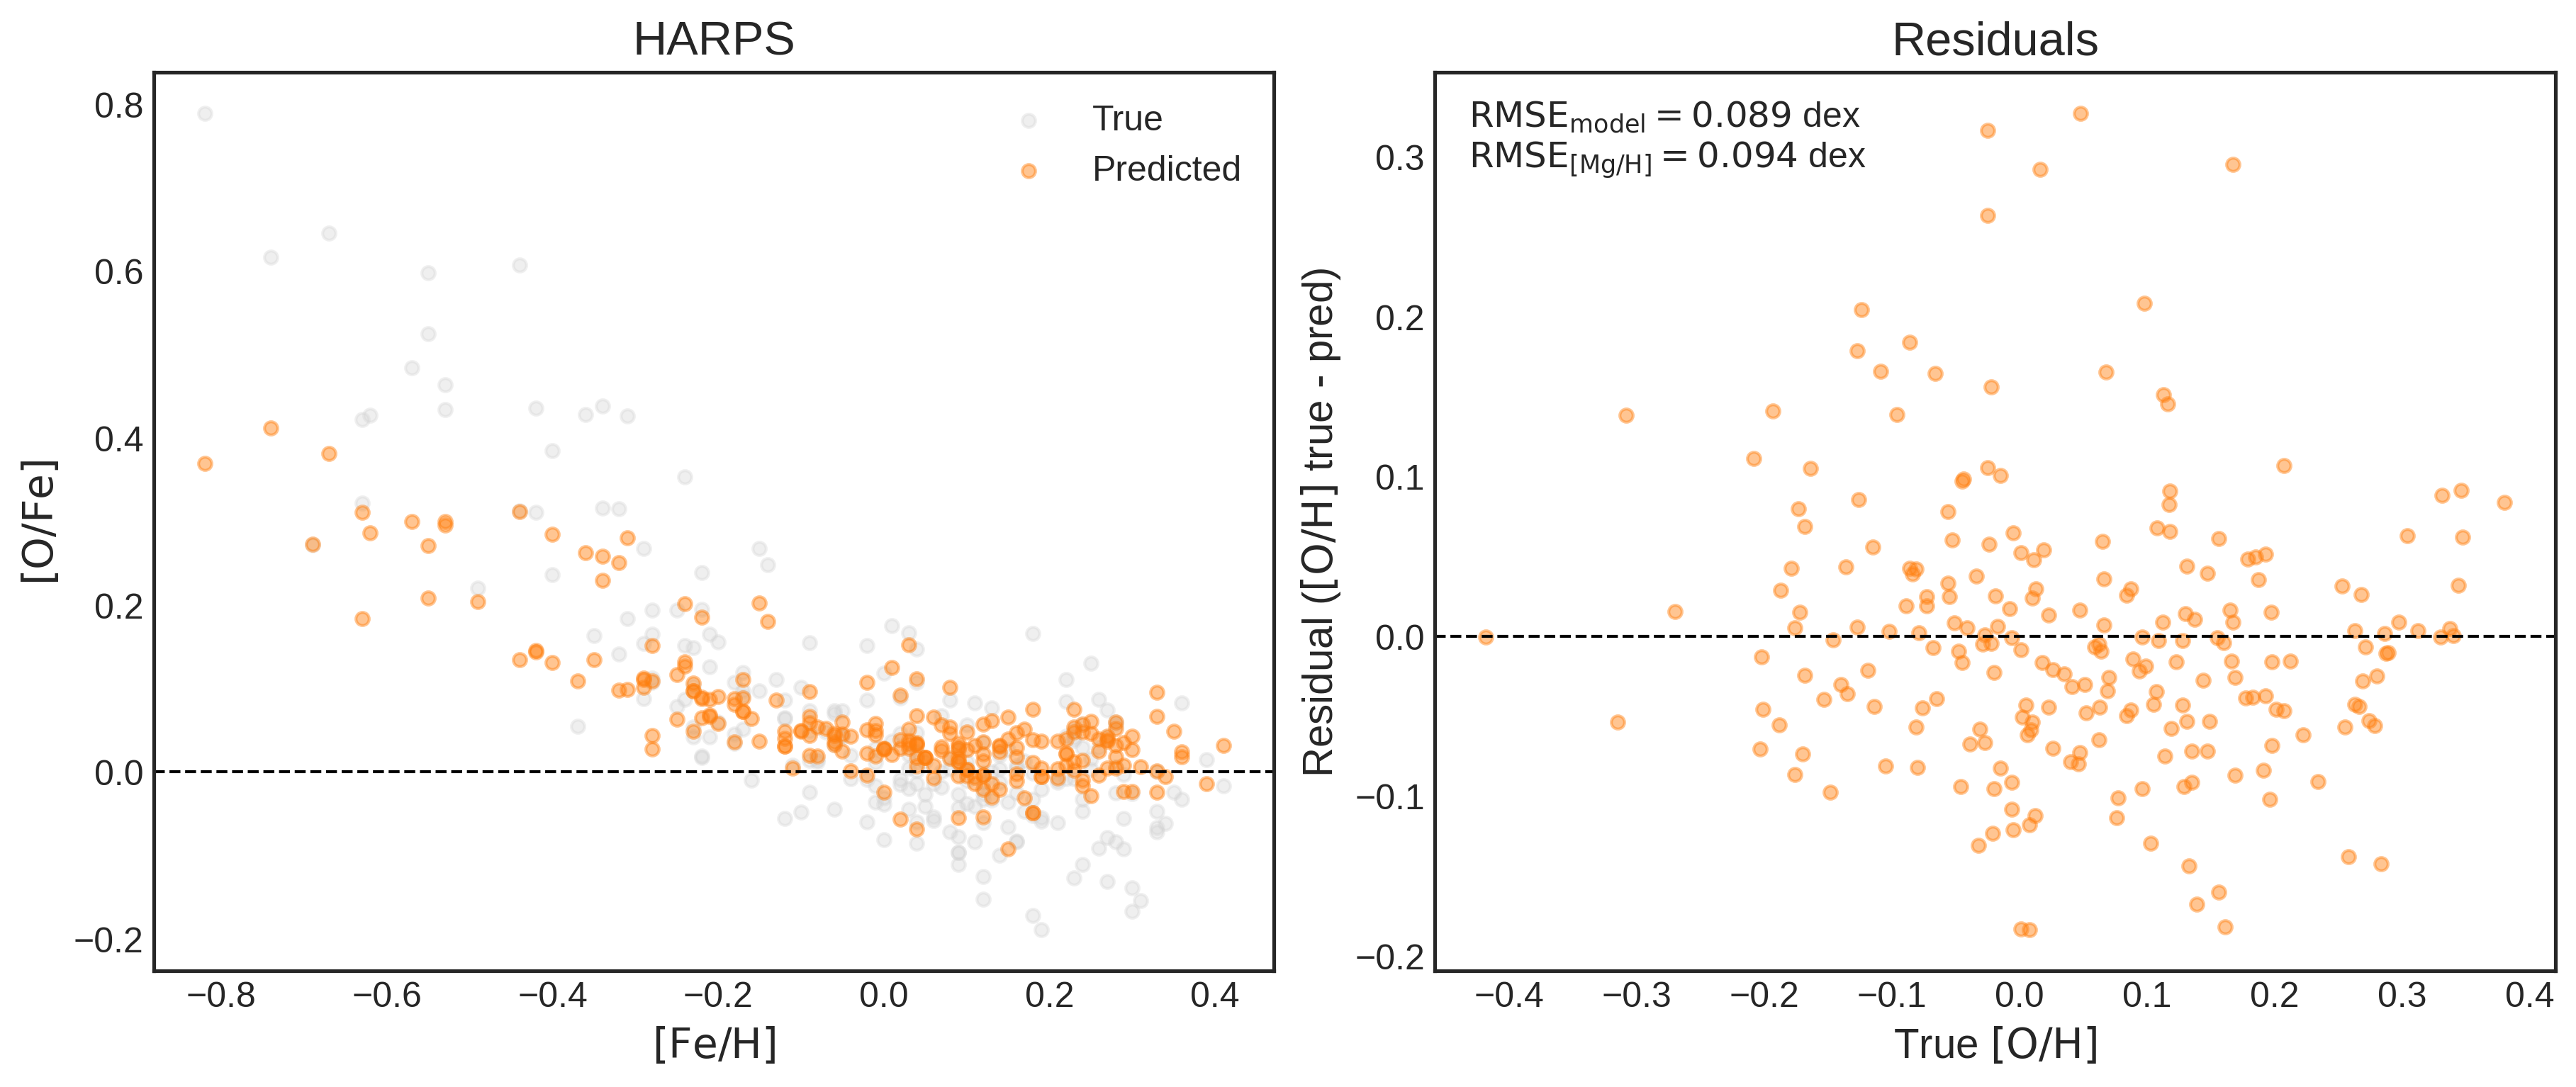
\includegraphics[width=0.48\textwidth]{figures/prediction_panels_harps_fe_mg_si_o_h.png}
\vspace{0.4cm}
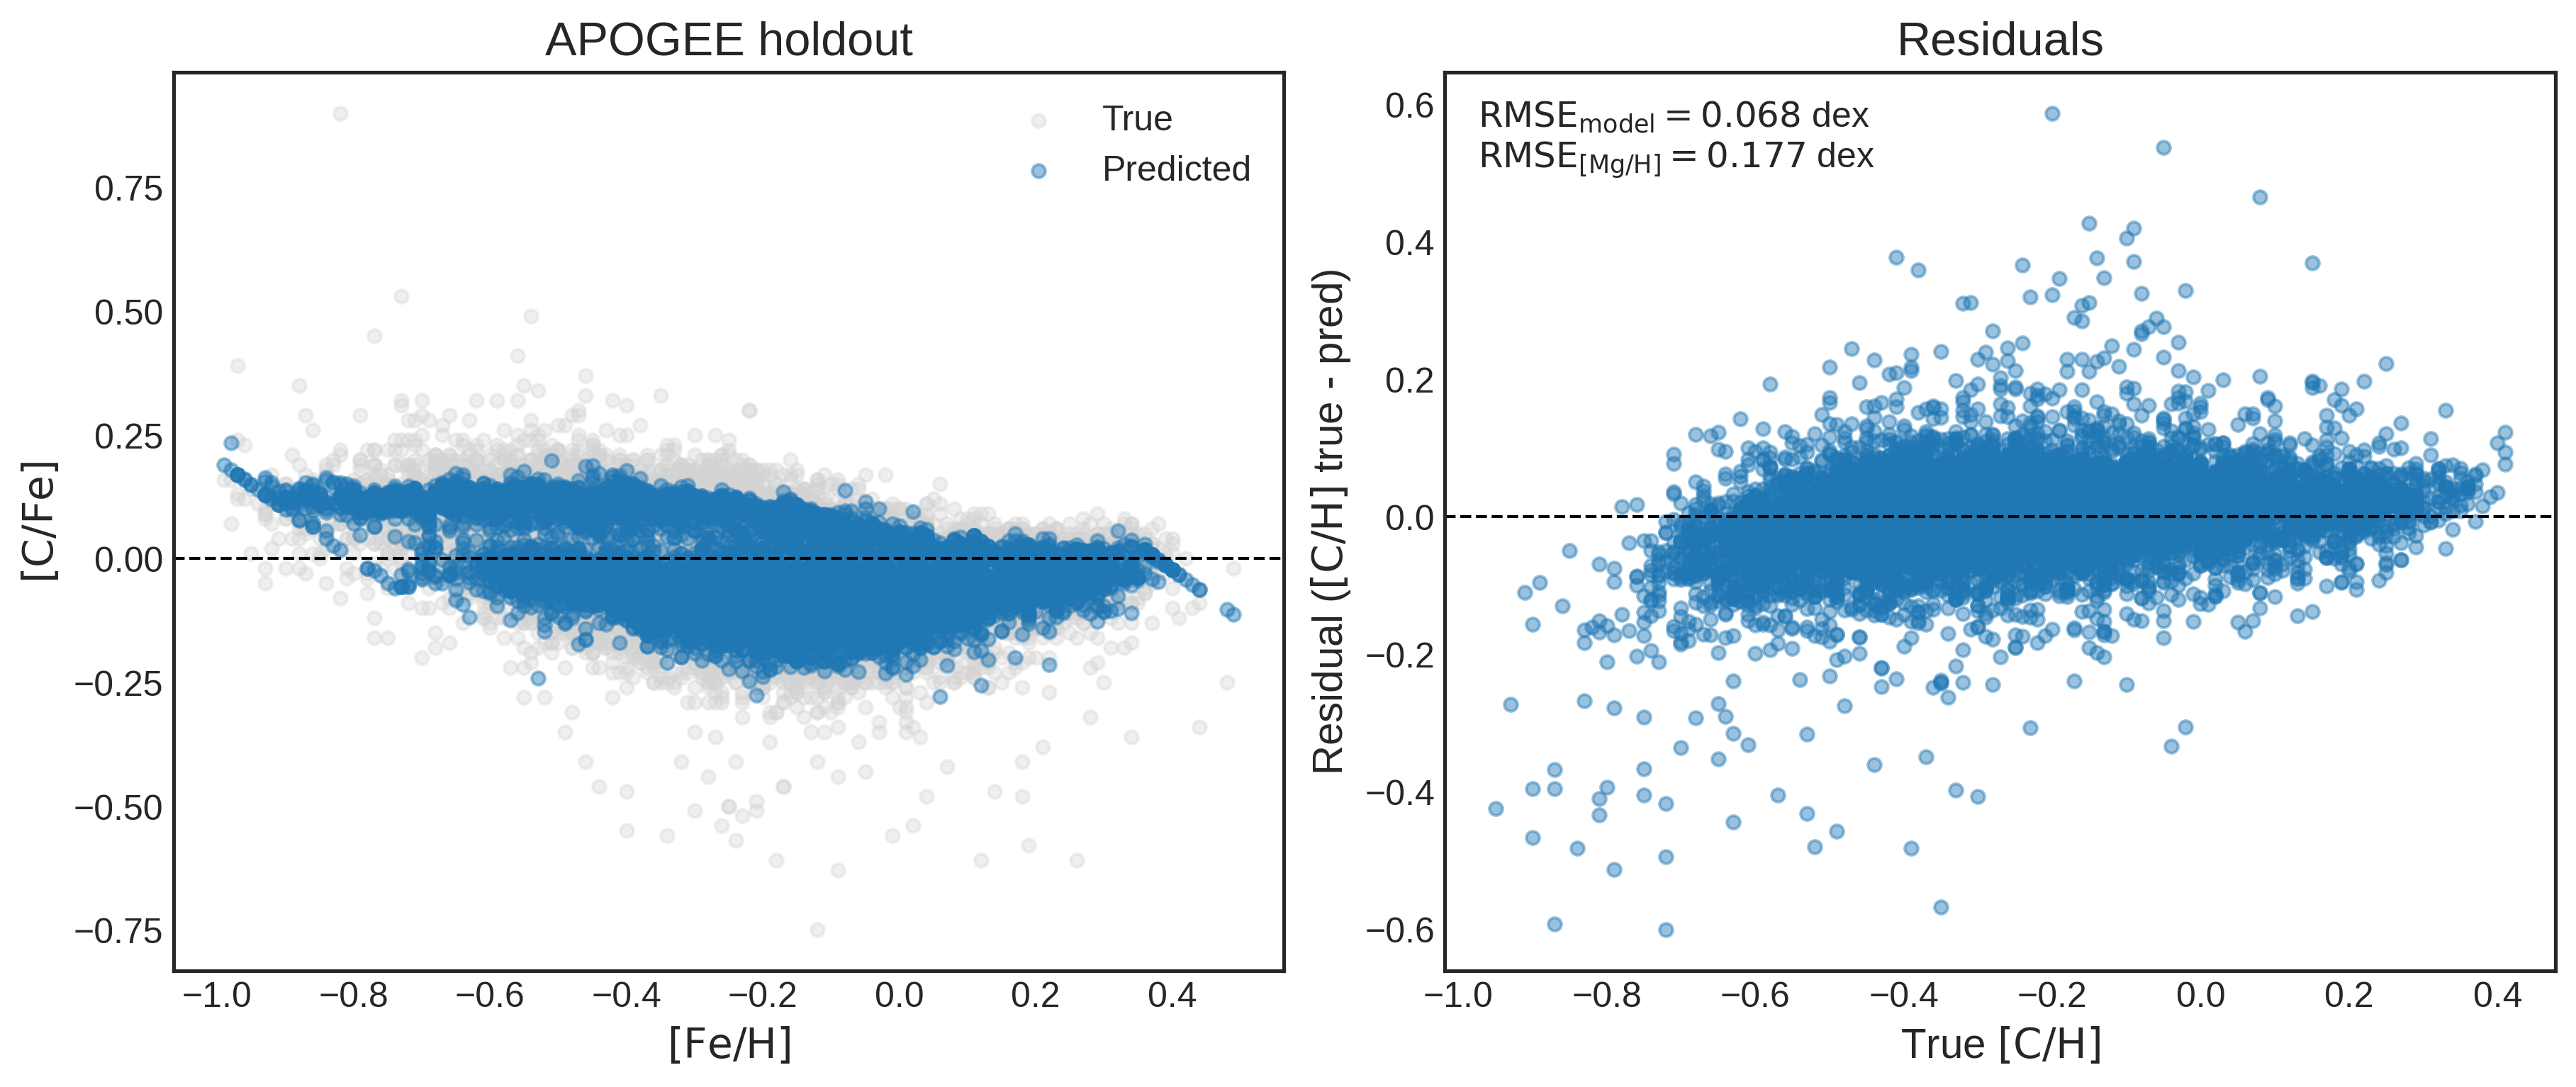
\includegraphics[width=0.48\textwidth]{figures/prediction_panels_apogee_holdout_fe_mg_si_c_h.png}
\hfill
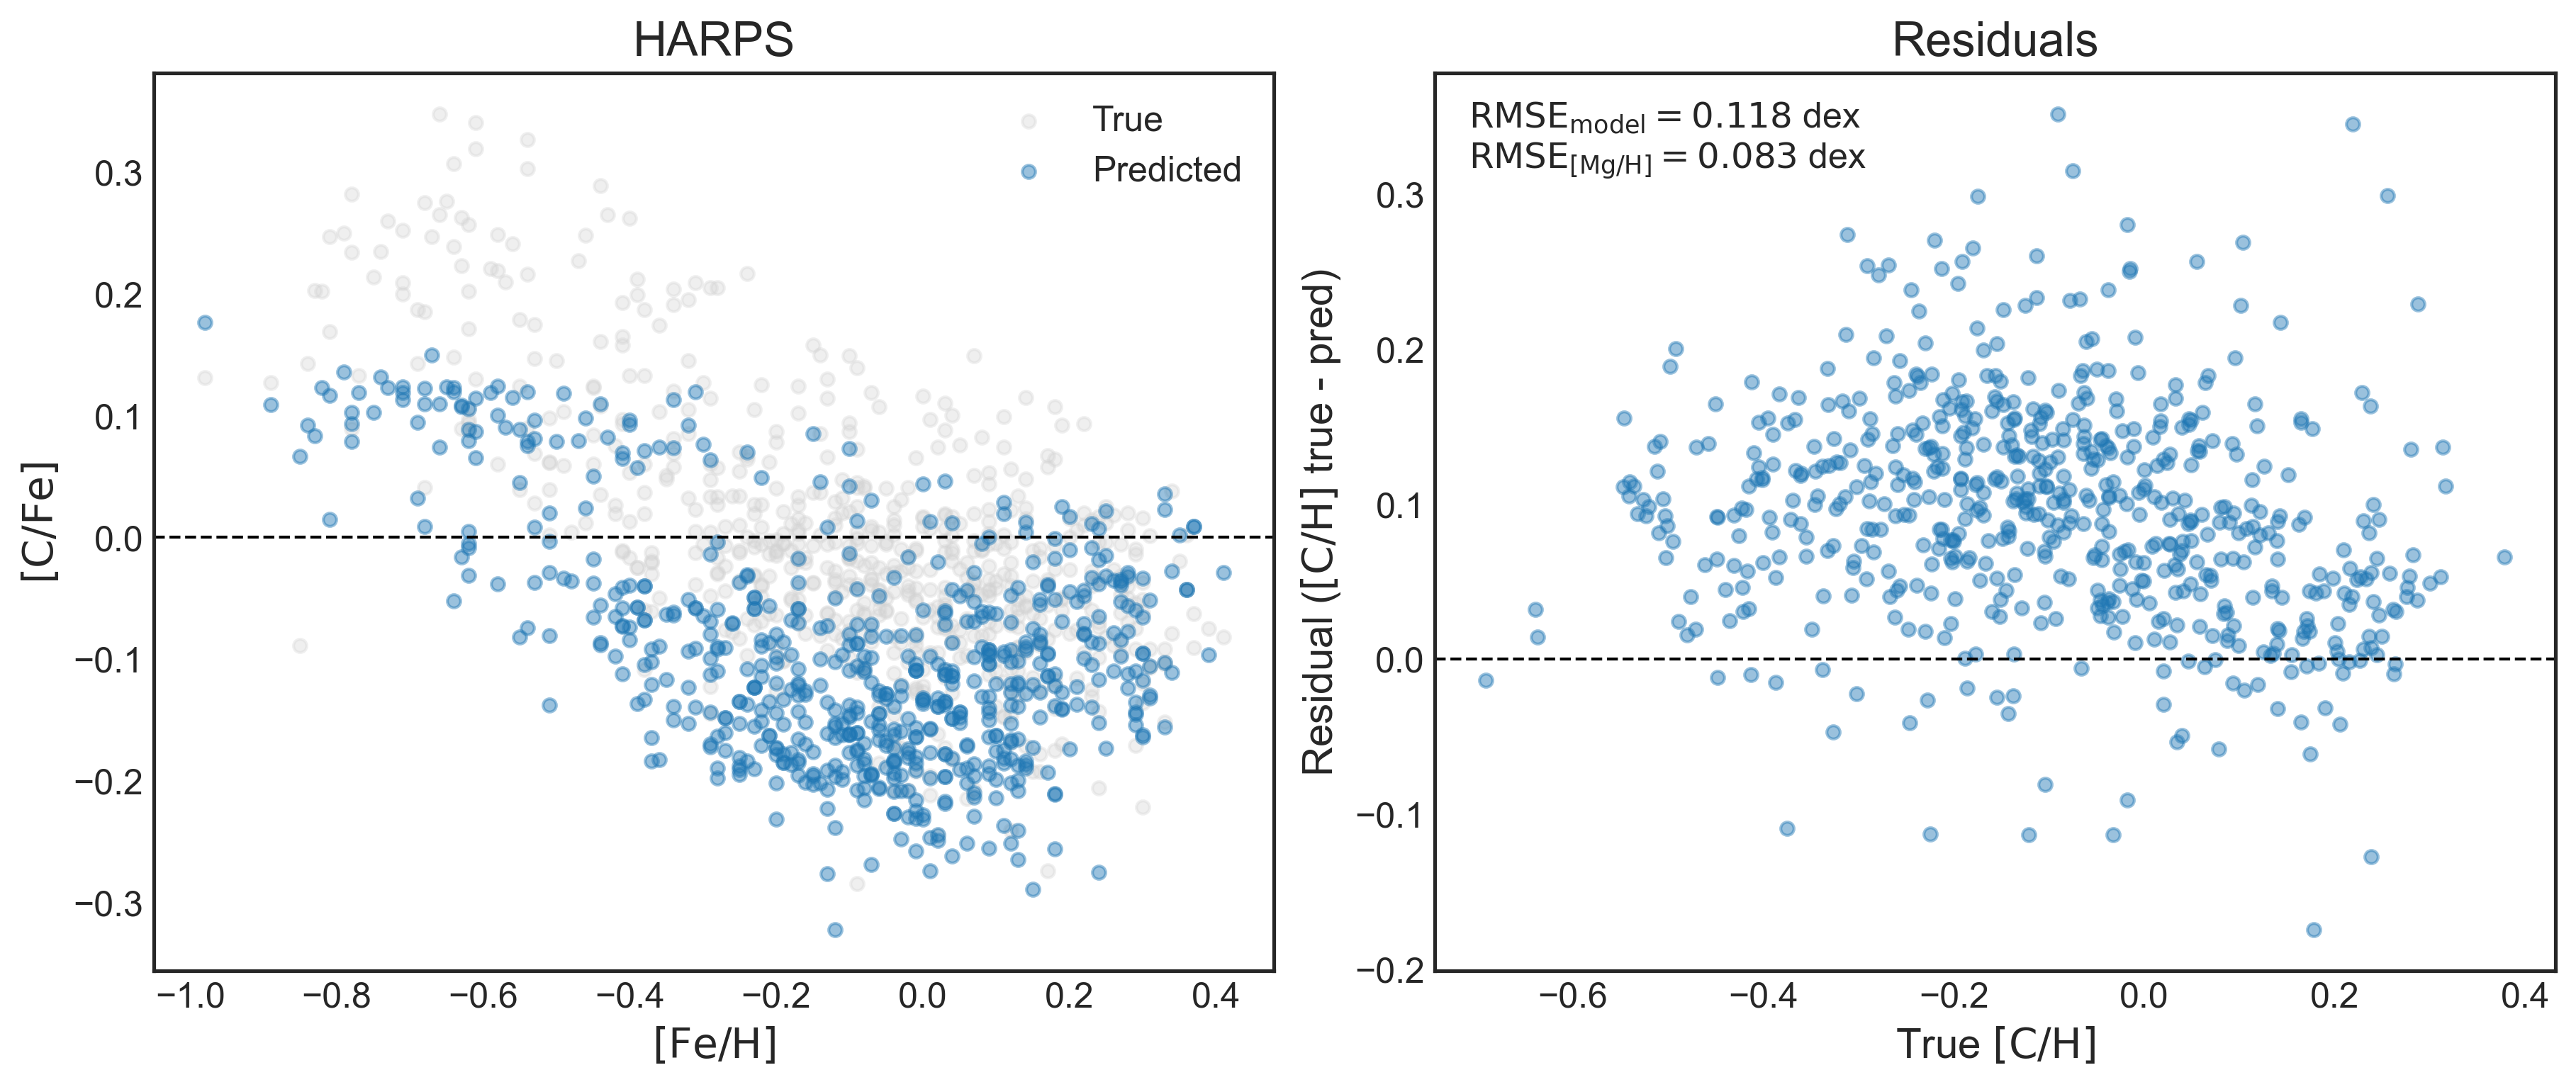
\includegraphics[width=0.48\textwidth]{figures/prediction_panels_harps_fe_mg_si_c_h.png}
\caption{Same as Fig.~\ref{fig:abundance_predictions}, but for the prediction of C and O abundances from Mg, Si, and [Fe/H].}
\label{fig:CO_predictions}
\end{figure*}


\section{Abundance ratios relevant for exoplanet research} \label{sec:ratio_metallicity_trends}

In addition to the machine-learning experiments described above, we explored the empirical behaviour of several abundance ratios that are particularly relevant for exoplanet composition studies. The purpose of this exercise is to provide a quick and simple way of obtaining these ratios just from metallicity. Using the APOGEE and HARPS samples separately, we examined the linear abundance ratios Fe/Si, Mg/Si, C/O, and Fe/O as a function of metallicity, [Fe/H]. The uncertainties on the fitted parameters were estimated by bootstrap resampling. In addition to the slope and intercept uncertainties (which were very small) we also computed the rms scatter around each best-fit relation over the full metallicity range considered.

The resulting trends are shown in Fig.~\ref{fig:ratio_fits_feh}, while the fitted slopes and rms scatter values are listed in Table~\ref{tab:ratio_slopes_rms}.  While some differences are observed between the two samples. Fe/Si and Fe/O increase with metallicity in both APOGEE and HARPS, whereas Mg/Si decreases with increasing [Fe/H]. The C/O ratio also increases with metallicity in both datasets. The qualitative behaviour of the fits for the two samples is similar, although the fitted slopes are not identical. However, the differences are within the rms scatter of the samples. In particular, the largest fractional offset between the two empirical relations at the whole range of metallicity is less than 20\%.


\begin{figure*}[ht]
    \centering
    \begin{subfigure}{0.49\textwidth}
        \centering
        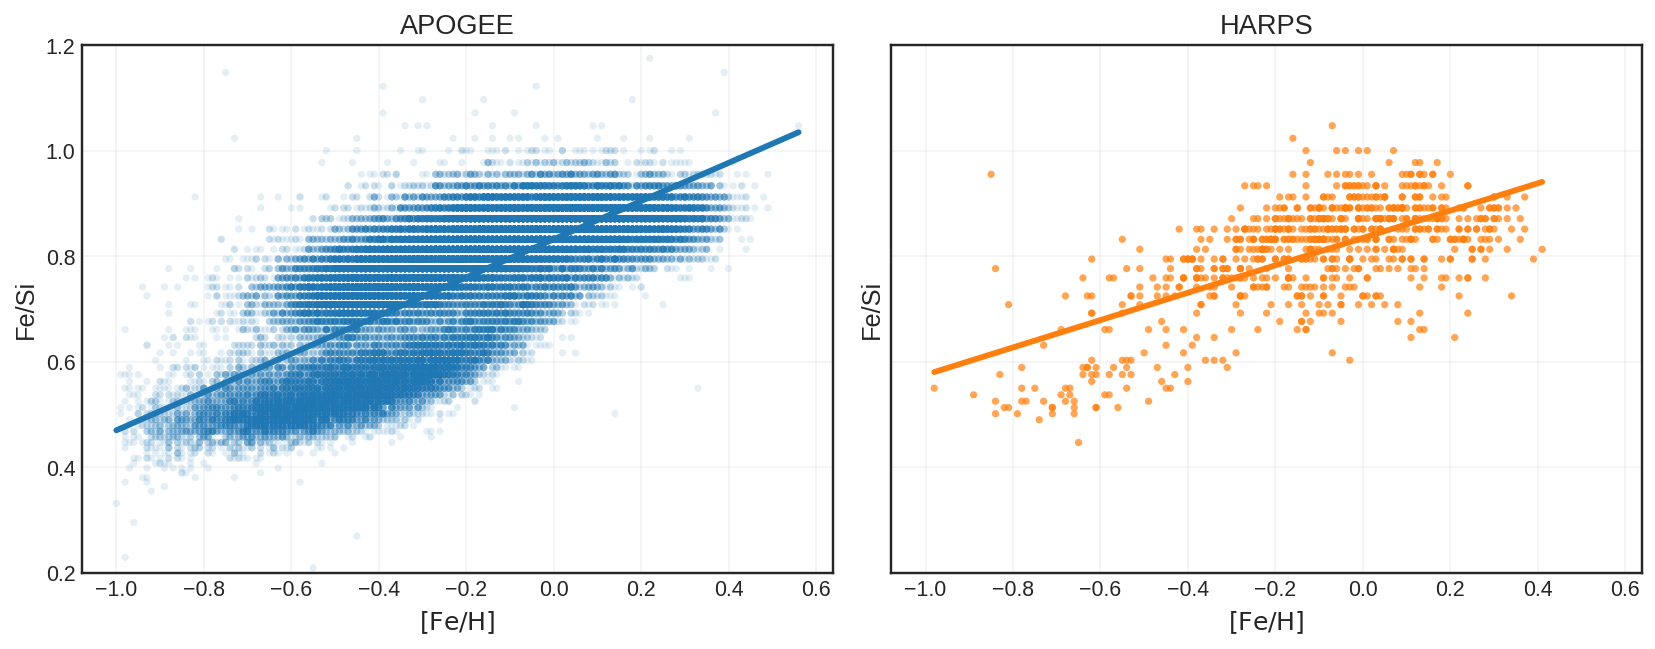
\includegraphics[width=\linewidth]{figures/linear_fe_si_vs_feh.png}
    \end{subfigure}
    \hfill
    \begin{subfigure}{0.49\textwidth}
        \centering
        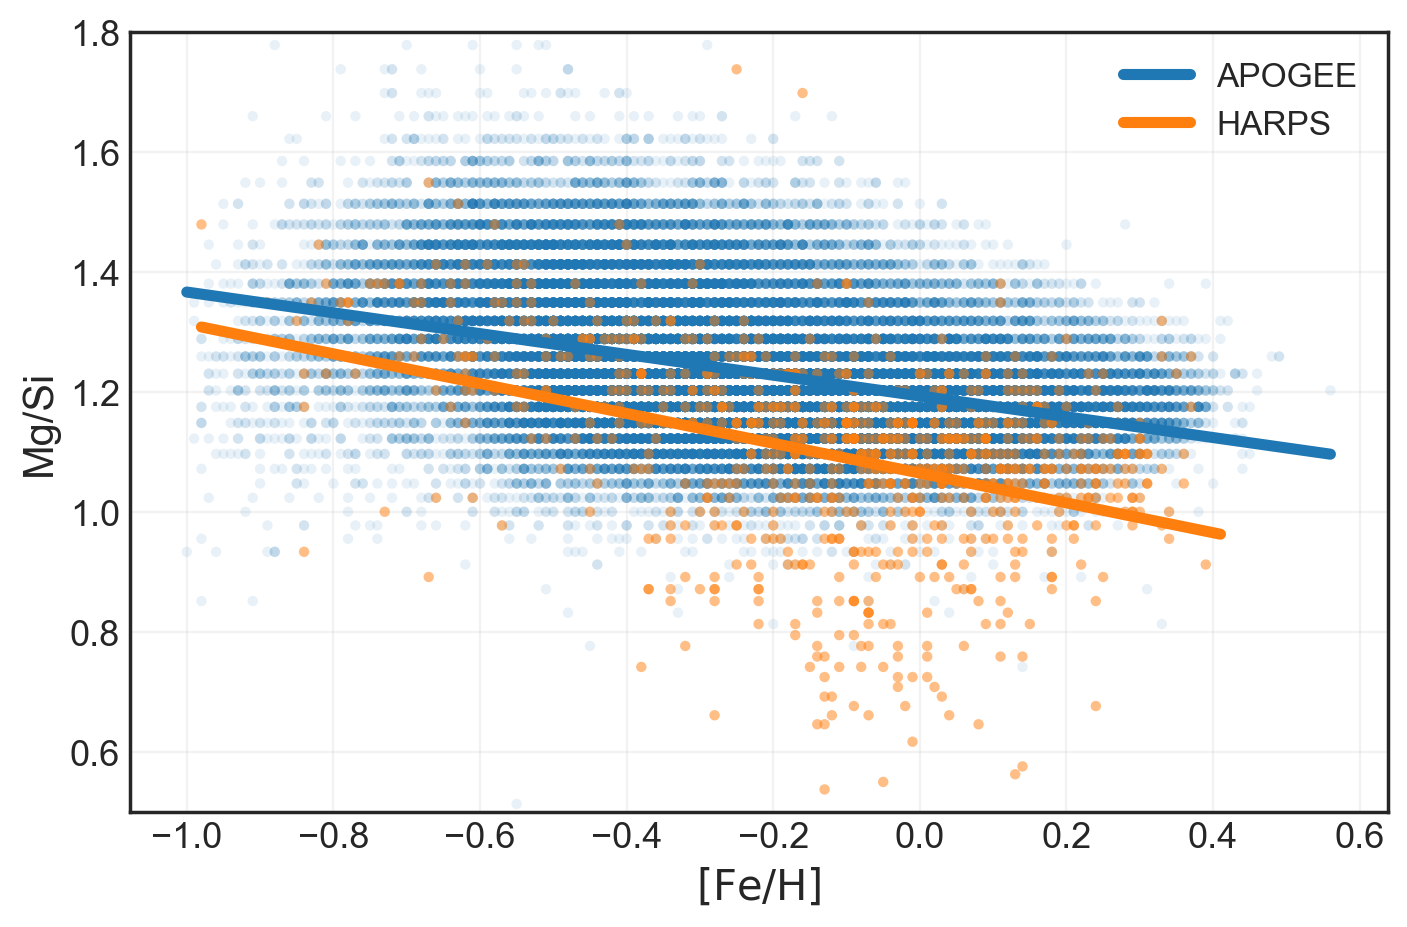
\includegraphics[width=\linewidth]{figures/linear_mg_si_vs_feh.png}
    \end{subfigure}

    \vspace{0.5em}

    \begin{subfigure}{0.49\textwidth}
        \centering
        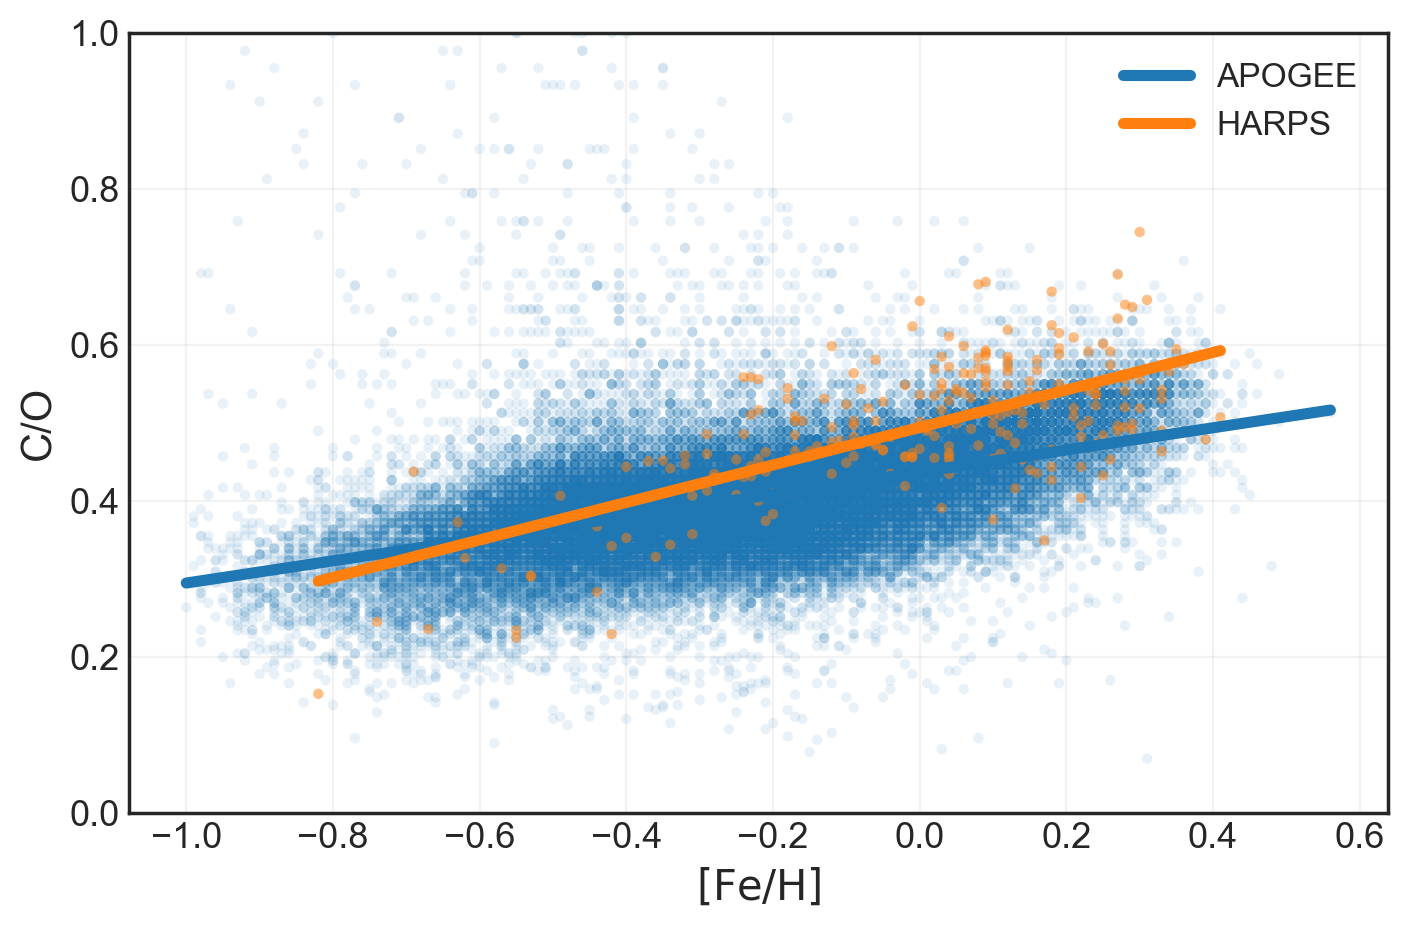
\includegraphics[width=\linewidth]{figures/linear_c_o_vs_feh.png}
    \end{subfigure}
    \hfill
    \begin{subfigure}{0.49\textwidth}
        \centering
        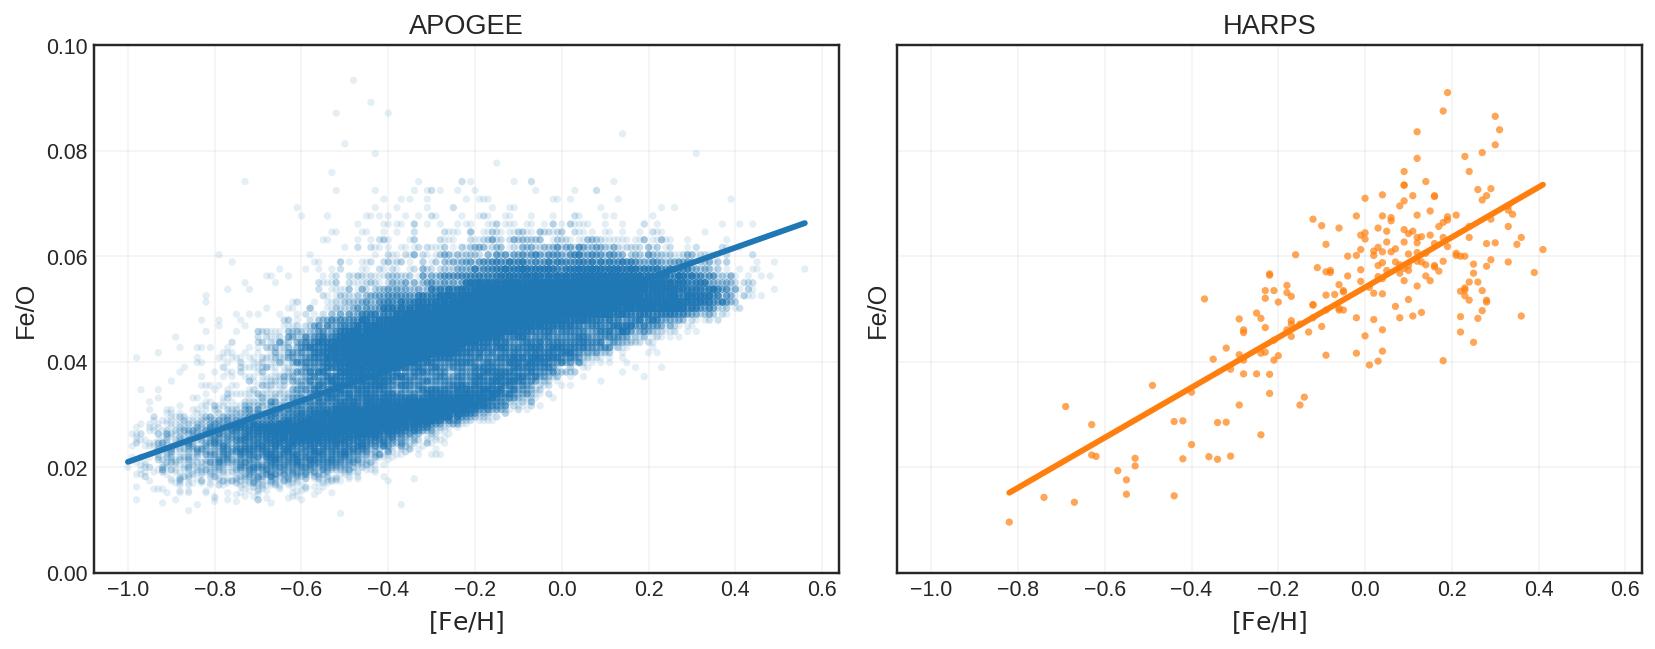
\includegraphics[width=\linewidth]{figures/linear_fe_o_vs_feh.png}
    \end{subfigure}
    \caption{Linear abundance ratios as a function of metallicity for the APOGEE and HARPS samples. In each panel, the left and right subplots show the APOGEE and HARPS data, respectively, together with the corresponding best-fit linear relation.}
    \label{fig:ratio_fits_feh}
\end{figure*}



\begin{table*}
\caption{Linear fits of abundance ratios as a function of metallicity for the APOGEE and HARPS samples.}
\label{tab:ratio_slopes_rms}
\centering
\small
\begin{tabular}{lllc}
\hline\hline
Survey & Ratio & Equation & RMS scatter \\
\hline
APOGEE & Fe/Si & $y = (0.8319 \pm 0.0005) + (0.3622 \pm 0.0014)\,[\mathrm{Fe/H}]$ & 0.09 \\
HARPS & Fe/Si & $y = (0.8343 \pm 0.0027) + (0.2593 \pm 0.0132)\,[\mathrm{Fe/H}]$ & 0.08 \\
APOGEE & Mg/Si & $y = (1.1931 \pm 0.0006) + (-0.1733 \pm 0.0019)\,[\mathrm{Fe/H}]$ & 0.11 \\
HARPS & Mg/Si & $y = (1.0645 \pm 0.0059) + (-0.2486 \pm 0.0183)\,[\mathrm{Fe/H}]$ & 0.15 \\
APOGEE & C/O & $y = (0.4367 \pm 0.0004) + (0.1422 \pm 0.0016)\,[\mathrm{Fe/H}]$ & 0.07 \\
HARPS & C/O & $y = (0.4941 \pm 0.0046) + (0.2405 \pm 0.0225)\,[\mathrm{Fe/H}]$ & 0.06 \\
APOGEE & Fe/O & $y = (0.0500 \pm 0.0000) + (0.0290 \pm 0.0001)\,[\mathrm{Fe/H}]$ & 0.007 \\
HARPS & Fe/O & $y = (0.0541 \pm 0.0006) + (0.0475 \pm 0.0027)\,[\mathrm{Fe/H}]$ & 0.009 \\
\hline
\end{tabular}
\end{table*}

\section{Predicted abundances of planet host stars}

As a practical application of the developed framework, we applied the trained models to planet-host stars from SWEET-Cat, one of the largest catalogues of stars with homogeneous atmospheric parameters in exoplanet systems. For these stars we combined the published SWEET-Cat metallicities with \textit{Gaia} DR3 astrometry and radial velocities to derive Galactic velocities and orbital parameters in the same way as for the training samples.

Using these inputs, we predicted the abundances of C, O, Mg, and Si for SWEET-Cat stars lacking homogeneous determinations of these quantities. From the predicted abundances we further derived the abundance ratios Fe/Si, Mg/Si, C/O, and Fe/O, which are particularly relevant for interpreting the bulk composition and mineralogy of exoplanets. In parallel, we evaluated the simple linear abundance-ratio relations derived from APOGEE and HARPS as a function of [Fe/H], providing an alternative low-dimensional approximation when only metallicity is available.

This application illustrates the main practical value of our approach. Even when direct abundance measurements are unavailable or difficult to obtain, one can combine metallicity with kinematic information to estimate chemically informative quantities for planet-host stars and to place them in the broader context of Galactic chemical evolution.

\section{Conclusion and summary}

We have investigated how far stellar metallicity and individual abundances can be inferred from kinematics, orbital properties, and a limited set of elemental abundances. APOGEE was used as the main training set, while HARPS provided an external and chemically precise validation sample. Our main conclusions are as follows.

Kinematic information alone contains significant, although limited, predictive power for stellar metallicity. Gradient-boosting models reach an RMSE of about 0.20 dex on APOGEE and about 0.22 dex on the independent HARPS sample. Across all feature-importance diagnostics, $Z_{\max}$ emerges as the dominant predictor, showing that the vertical extent of stellar orbits carries the strongest dynamical imprint of metallicity in our analysis.

When [Fe/H] is included among the predictors, the abundances of C, O, Mg, and Si can be estimated much more accurately than with the simple approximation $\mathrm{[X/H]}=\mathrm{[Fe/H]}$. In these models, metallicity is by far the main driver of the predictions, while orbital properties such as $R_{\mathrm{peri}}$ and $Z_{\max}$ provide secondary but measurable additional information. The gain relative to the baseline demonstrates that kinematics can refine abundance estimates even when metallicity is already known.

C and O can also be inferred from Mg, Si, and [Fe/H] with useful precision. In this case, adding kinematic information does not materially improve the predictions, implying that most of the relevant information is already encoded in the elemental abundances themselves, especially Mg. The main limitation when transferring the models to an external sample is not model flexibility, but systematic differences between abundance scales, most clearly seen for carbon.

In addition to the machine-learning models, we derived simple linear relations between the abundance ratios Fe/Si, Mg/Si, C/O, and Fe/O and stellar metallicity for both APOGEE and HARPS. These relations do not replace the full predictive models, but they provide a compact and practical approximation for applications in which only [Fe/H] is available.

Overall, our results show that machine-learning models trained on spectroscopic surveys can provide a practical route to estimating chemically informative quantities for stars whose detailed abundances are difficult to measure directly, including many exoplanet hosts. At the same time, the limited gains obtained from trying a wide range of algorithms and feature-engineering strategies indicate that future progress will depend primarily on the quality, homogeneity, and physical informativeness of the available input data rather than on further increases in model complexity.

%comparison between the surveys https://ui.adsabs.harvard.edu/abs/2023A%26A...670A.107H/abstract
%%%%%%%%%%%%%%%%%%%%%%%%%%%%%%%%%%%%%%%%%%%%%%%%%%%%%%%%%%%%%%
\begin{acknowledgements}
V.~A. acknowledges support from FCT – Funda\c{c}\~ao para a Ci\^encia e Tecnologia through national funds and from FEDER via COMPETE2020 – Programa Operacional Competitividade e Internacionalização, under the grants UIDB/04434/2020 (DOI: 10.54499/UIDB/04434/2020) and UIDP/04434/2020 (DOI: 10.54499/UIDP/04434/2020), as well as through a work contract funded by the FCT Scientific Employment Stimulus program (reference 2023.06055.CEECIND/CP2839/CT0005, DOI: 10.54499/2023.06055.CEECIND/CP2839/CT0005).
\end{acknowledgements}




%%%%%%%%%%%%%%%%%%%%%%%%%%%%%%%%%%%%%%%%%%%%%%%%%%%%%%%%%%%%%%
% WARNING
% Please note that we have included the references below in
% order to compile the document, but we ask you to:
%
% - use BibTeX with the regular commands:
\bibliographystyle{aa} % style aa.bst
\bibliography{references} % your references Yourfile.bib


%%%%%%%%%%%%%%%%%%%%%%%%%%%%%%%%%%%%%%%%%%%%%%%%%%%%%%%%%%%%%%%
% Appendices must be placed after   \end{thebibliography}
% They will be placed automatically on a new page.
%%%%%%%%%%%%%%%%%%%%%%%%%%%%%%%%%%%%%%%%%%%%%%%%%%%%%%%%%%%%%%%
\begin{appendix}

\section{Construction of the samples} \label{target_selection}

In this section, we describe in detail the selection criteria adopted for the different samples and the determination of the relevant parameters.

\subsection{APOGEE DR17}

For the APOGEE sample, we performed a careful quality selection to ensure reliable stellar parameters and elemental abundances. We excluded stars with problematic \texttt{APOGEE\_STARFLAG} entries, removing objects affected by high persistence (\texttt{PERSIST\_HIGH}, bit~9), low signal-to-noise ratio (\texttt{LOW\_SNR}, bit~4), contamination from a very bright neighbor (\texttt{VERY\_BRIGHT\_NEIGHBOR}, bit~3), and spectra showing significant positive or negative persistence jumps in the blue chip (\texttt{PERSIST\_JUMP\_POS}, bit~12; \texttt{PERSIST\_JUMP\_NEG}, bit~13). We also excluded stars flagged as having inconsistent radial velocity determinations (\texttt{SUSPECT\_RV\_COMBINATION}, bit~16).

To ensure a homogeneous and representative dataset, we selected only stars belonging to the main APOGEE survey by requiring \texttt{EXTRATARG}~=~0, thereby excluding ancillary and calibration targets. Using the \texttt{PROGRAMNAME} flag, we further removed stars that were part of minor programs (those containing fewer than 1500 stars) targeting specific objects.

To guarantee robust stellar parameters, elemental abundances, and kinematic measurements, we applied the following additional selection criteria \citep[see e.g.,][]{Feltzing-23}: 
we retained only red giant stars with effective temperatures $4000 < T_{\mathrm{eff}} < 6000$~K, surface gravities $1.0 < \log g < 2.5$~dex, and spectra with signal-to-noise ratios $\mathrm{S/N} > 100$. We required that \texttt{FE\_H\_FLAG}~=~0 and \texttt{X\_FE\_FLAG}~=~0 for the key elements C, O, Mg, Si, and Fe, and that the uncertainties in the corresponding abundances be smaller than 0.05~dex. We further required relative parallax uncertainties $\sigma_\pi / \pi < 0.1$ to ensure reliable distances. 

Because the main motivation of the present work is to predict metallicities and abundances of exoplanet host stars, we restricted the sample to stars within the metallicity range $-1.0 < [\mathrm{Fe/H}] < 0.6$~dex. The upper limit was imposed to avoid unrealistically high values or chemically peculiar objects. We also verified that all selected stars possess measured radial velocities, \textit{Gaia} parallaxes, and proper motions, which were used to compute the kinematic properties of the sample.

After applying all the above selection criteria, the final APOGEE sample consists of about 46\,000 red giant stars.

%\subsection{GALAH DR4}

%Similar to the APOGEE sample, we also restricted the GALAH sample to stars with the most reliable stellar parameters and abundance determinations. We excluded stars with identified issues in their stellar parameter derivations by requiring \texttt{flag\_sp}~=~0. Only high-quality spectra were retained by selecting stars with \texttt{snr\_px\_ccd2}~$>$~50, corresponding to the SNR per pixel from the second GALAH camera. 

%We further limited the sample to FGK dwarf stars with  $5000 < T_{\mathrm{eff}} < 6300$~K and  $4.1 < \log g < 4.7$~dex. We required the metallicity and all relevant elemental abundance flags to be zero (e.g. \texttt{flag\_mg\_fe}~=~0), and the uncertainties in the abundances to be smaller than 0.1~dex. The metallicity range was restricted to $-1.0 < [\mathrm{Fe/H}] < 0.6$~dex to avoid metal-poor and chemically peculiar stars. 

%It is worth noting that the reported uncertainties in the GALAH abundances are systematically larger, as they account for both precision and accuracy effects \citep{Buder-25}. As for the APOGEE sample, we required relative parallax uncertainties $\sigma_\pi / \pi < 0.1$ to ensure reliable distance estimates.

%After applying all the above selection criteria, the final GALAH sample consists of approximately 71\,000 FGK dwarf stars.


\subsection{HARPS}

The HARPS sample consists of 798 FGK-type dwarf stars with homogeneously derived atmospheric parameters and elemental abundances \citep{Adibekyan-12, DelgadoMena-21}. The astrometric data for these stars were taken from \textit{Gaia}~DR3, and as for the other samples, we required relative parallax uncertainties $\sigma_\pi / \pi < 0.1$ to ensure reliable distances. 

The metallicities of the HARPS stars span the range $-1.0 < [\mathrm{Fe/H}] < 0.4$~dex. This sample, composed primarily of bright, nearby stars observed in the context of exoplanet searches, provides high-precision spectroscopic abundances and serves as an excellent benchmark for testing the machine learning models.


\subsection{Kinematics and dynamics of the stars}

Using the formulation of \citet{Johnson-87}, and combining the astrometric parameters and radial velocities of the stars, we computed the Galactic space velocity components ($U_{\mathrm{LSR}}$, $V_{\mathrm{LSR}}$, and $W_{\mathrm{LSR}}$) relative to the Local Standard of Rest (LSR). The solar motion with respect to the LSR was adopted from \citet{Schonrich-10}. 

We then estimated the probability of each star belonging to one of the three main Galactic stellar populations (the thin disk, thick disk, or halo) following the prescription of \citet{Reddy-06}. This method assumes that stars in the solar neighborhood can be described as a mixture of these three kinematic populations, each characterized by Gaussian velocity distributions in the $U$, $V$, and $W$ components \citep{Schwarzschild-1907}. 

To further characterize the stellar orbits, we used the \texttt{galpy} package \citep{Bovy-15} to compute orbital parameters within a realistic Milky Way gravitational potential. For each star, we derived the pericentric ($R_{\mathrm{peri}}$) and apocentric ($R_{\mathrm{apo}}$) distances, orbital eccentricity ($e$), and the maximum vertical distance from the Galactic plane ($Z_{\mathrm{max}}$). The orbit integration was carried out assuming the \texttt{MWPotential2014} model provided by \texttt{galpy}, integrating each orbit over several Galactic rotations. 

These quantities provide insight into the dynamical behavior and population membership of the stars, and the methodology has been extensively applied in previous works \citep[e.g.,][]{Adibekyan-12}.



\section{Predicting metallicity from kinematics}
\label{appendix:metallicity}

This appendix presents supplementary material related to the prediction of stellar metallicity from kinematic and orbital parameters. In particular, we provide the full set of correlation analyses and additional figures used to explore the relationships between metallicity and the input features considered in this work.


\subsection{Exploratory data analysis for metallicity determination}

In this section, we provide the detailed results of the exploratory data analysis (EDA) performed to characterize the statistical relationships between the selected parameters and stellar metallicity.


\subsubsection{Spearman rank correlation analysis}

We computed Spearman’s rank correlation coefficient $\rho$ between each kinematic feature and [Fe/H] separately for the APOGEE and HARPS samples. Spearman’s coefficient measures monotonic associations without assuming linearity.

Figure~\ref{fig:spearman_appendix} presents the full set of correlation coefficients. In both samples, $Z_{\max}$ exhibits the strongest negative correlation with metallicity, while $P_{\rm gal}$ shows the strongest positive correlation. The next most correlated parameters are the orbital eccentricity $e$ and the total space velocity $\mathrm{UVW_{LSR}}$.

Although the absolute values of the coefficients differ slightly between APOGEE and HARPS—likely due to differences in stellar populations and sample size—the overall ranking of highly correlated features remains consistent.

\begin{figure*}
    \centering
    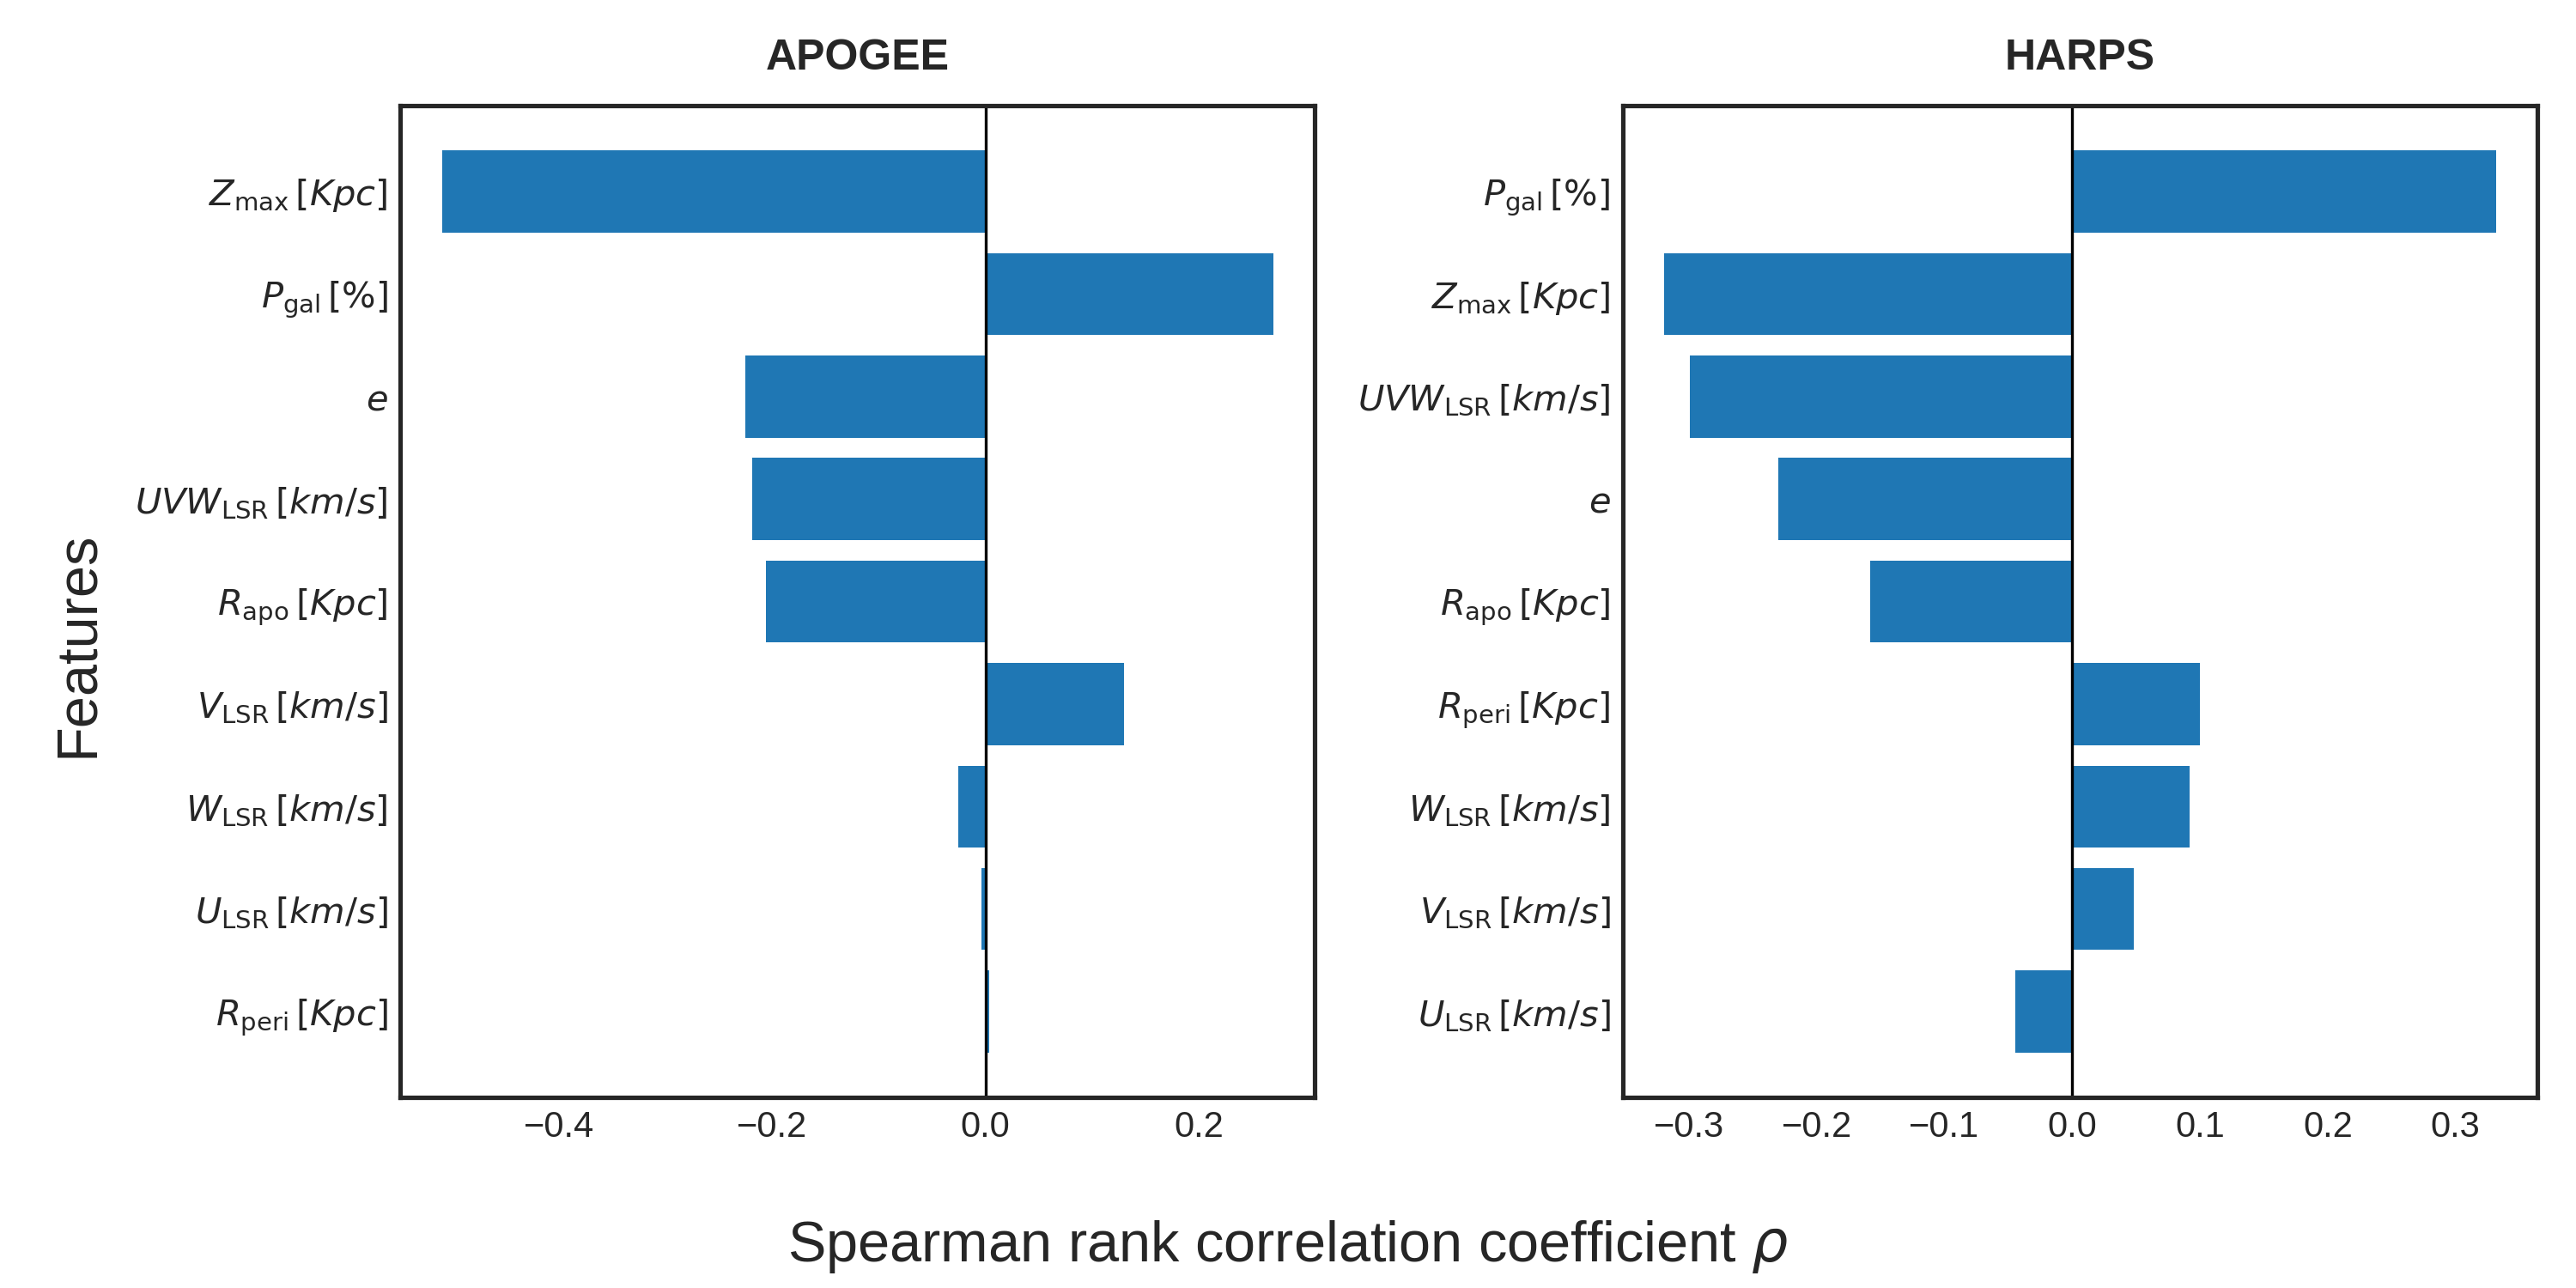
\includegraphics[width=0.8\textwidth]{correlations.png}
    \caption{Spearman rank correlation coefficients between the parameters and [Fe/H] for the APOGEE (left) and HARPS (right) samples.}
    \label{fig:spearman_appendix}
\end{figure*}


\subsubsection{Mutual information analysis}

To quantify nonlinear dependencies between the kinematic parameters and metallicity,
we computed the mutual information (MI) between each feature and [Fe/H].
Mutual information measures the general statistical dependence between two variables. Unlike correlation coefficients, MI does not assume linearity or monotonicity and is sensitive to arbitrary nonlinear relationships.

An MI value of zero indicates statistical independence, while larger values imply stronger dependence. In this work, MI was estimated using a non-parametric k-nearest-neighbour approach (with $k$ = 3), which is well suited for continuous variables \citep{kraskov2004}.


The MI values for both samples are shown in Figure~\ref{fig:mi_vif_appendix}. Consistent with the correlation analysis, $Z_{\max}$ and $P_{\rm gal}$ (also eccentricity) contain the largest amount of predictive information.

In addition, parameters such as $R_{\rm peri}$ show enhanced importance in the MI analysis compared to its rank correlation, suggesting the presence of nonlinear contributions to the metallicity-kinematics relation.



\subsubsection{Multicollinearity diagnostics}

We evaluated multicollinearity among the predictors using the variance inflation factor (VIF), defined as
\begin{equation}
\mathrm{VIF}_j = \frac{1}{1 - R_j^2},
\end{equation}
where $R_j^2$ is obtained by regressing feature $j$ against all remaining predictors. The VIF quantifies how much the variance of a regression coefficient is inflated due to linear dependence among input variables.

A VIF value of 1 indicates no multicollinearity, values between 1 and 5 are generally considered mild, values above 5 indicate moderate collinearity, and values exceeding 10 are typically interpreted as substantial multicollinearity.

High multicollinearity can lead to unstable coefficient estimates and inflated variance in linear models. However, its impact depends on the nature of the predictive algorithm. Tree-based ensemble methods, which perform recursive partitioning rather than coefficient estimation, are generally more robust to correlated predictors.

The resulting VIF values are shown in Figure~\ref{fig:mi_vif_appendix}. As expected, several parameters exhibit large VIF values due to their deterministic dependence on the other parameters. $Z_{\max}$ and $P_{\rm gal}$ display comparatively lower VIF values, indicating that they are not strongly linearly redundant with the remaining parameters.

\begin{figure}
    \centering
    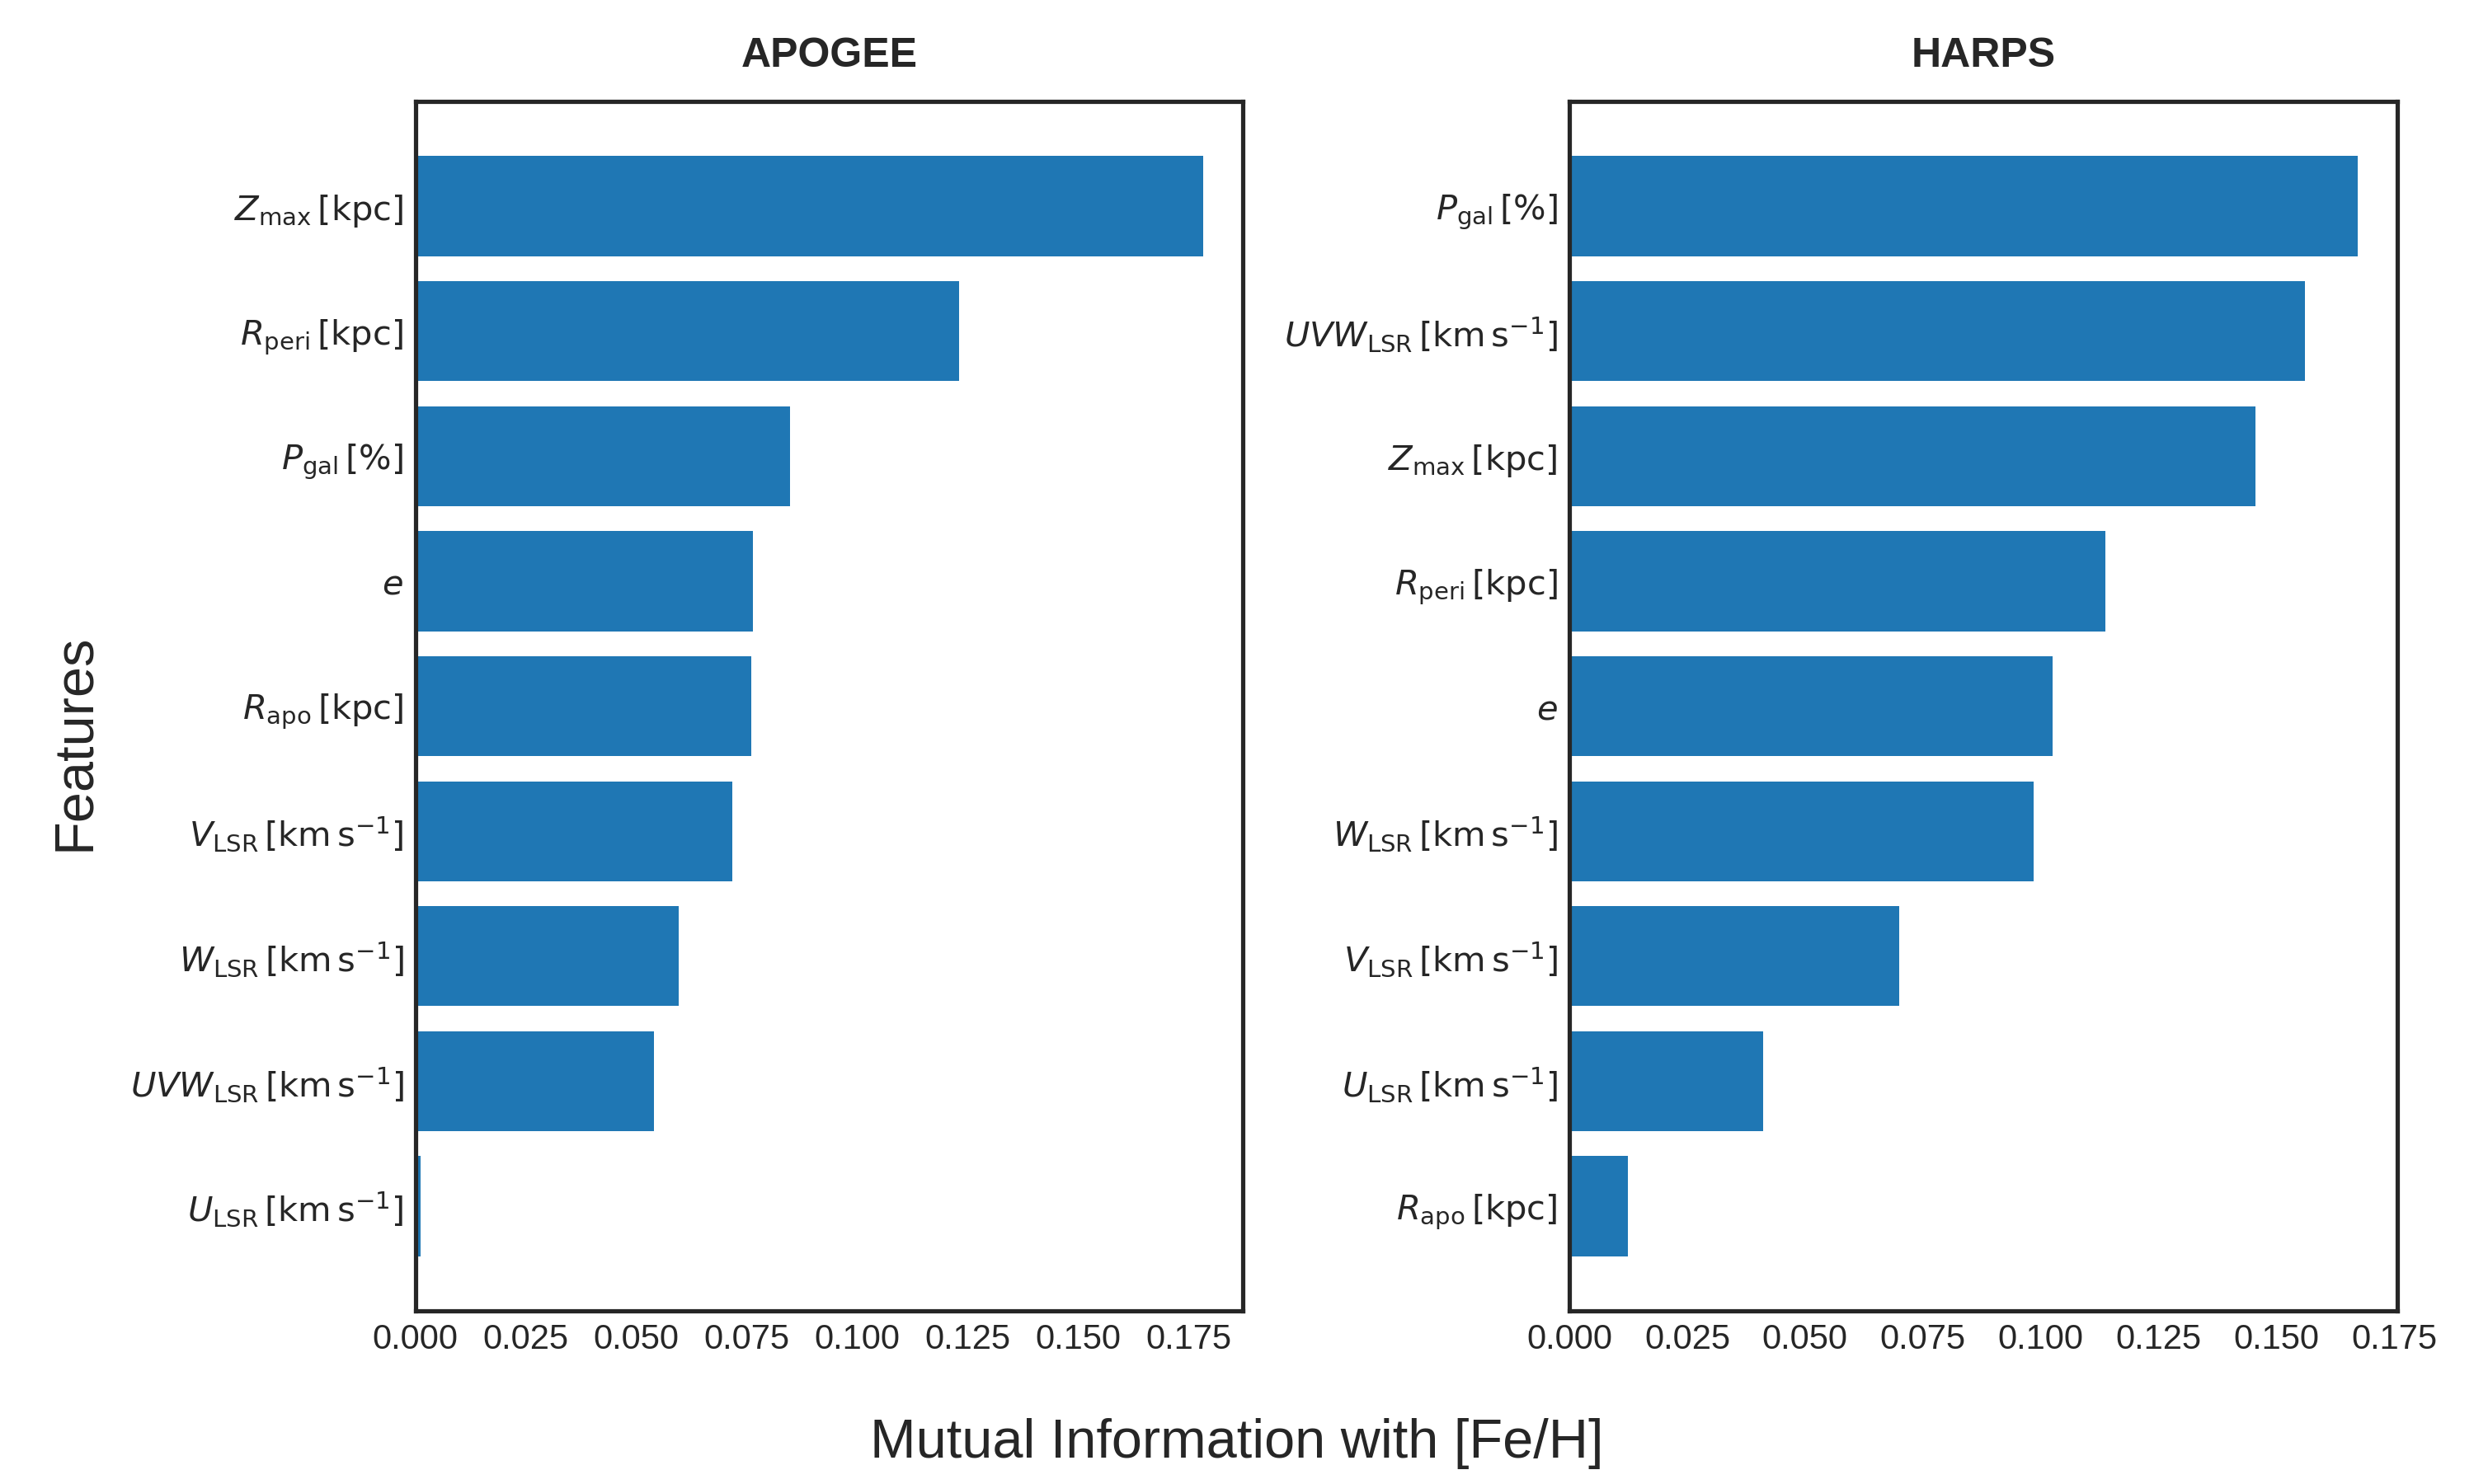
\includegraphics[width=0.49\textwidth]{MI.png}
    \vspace{0.4cm}
    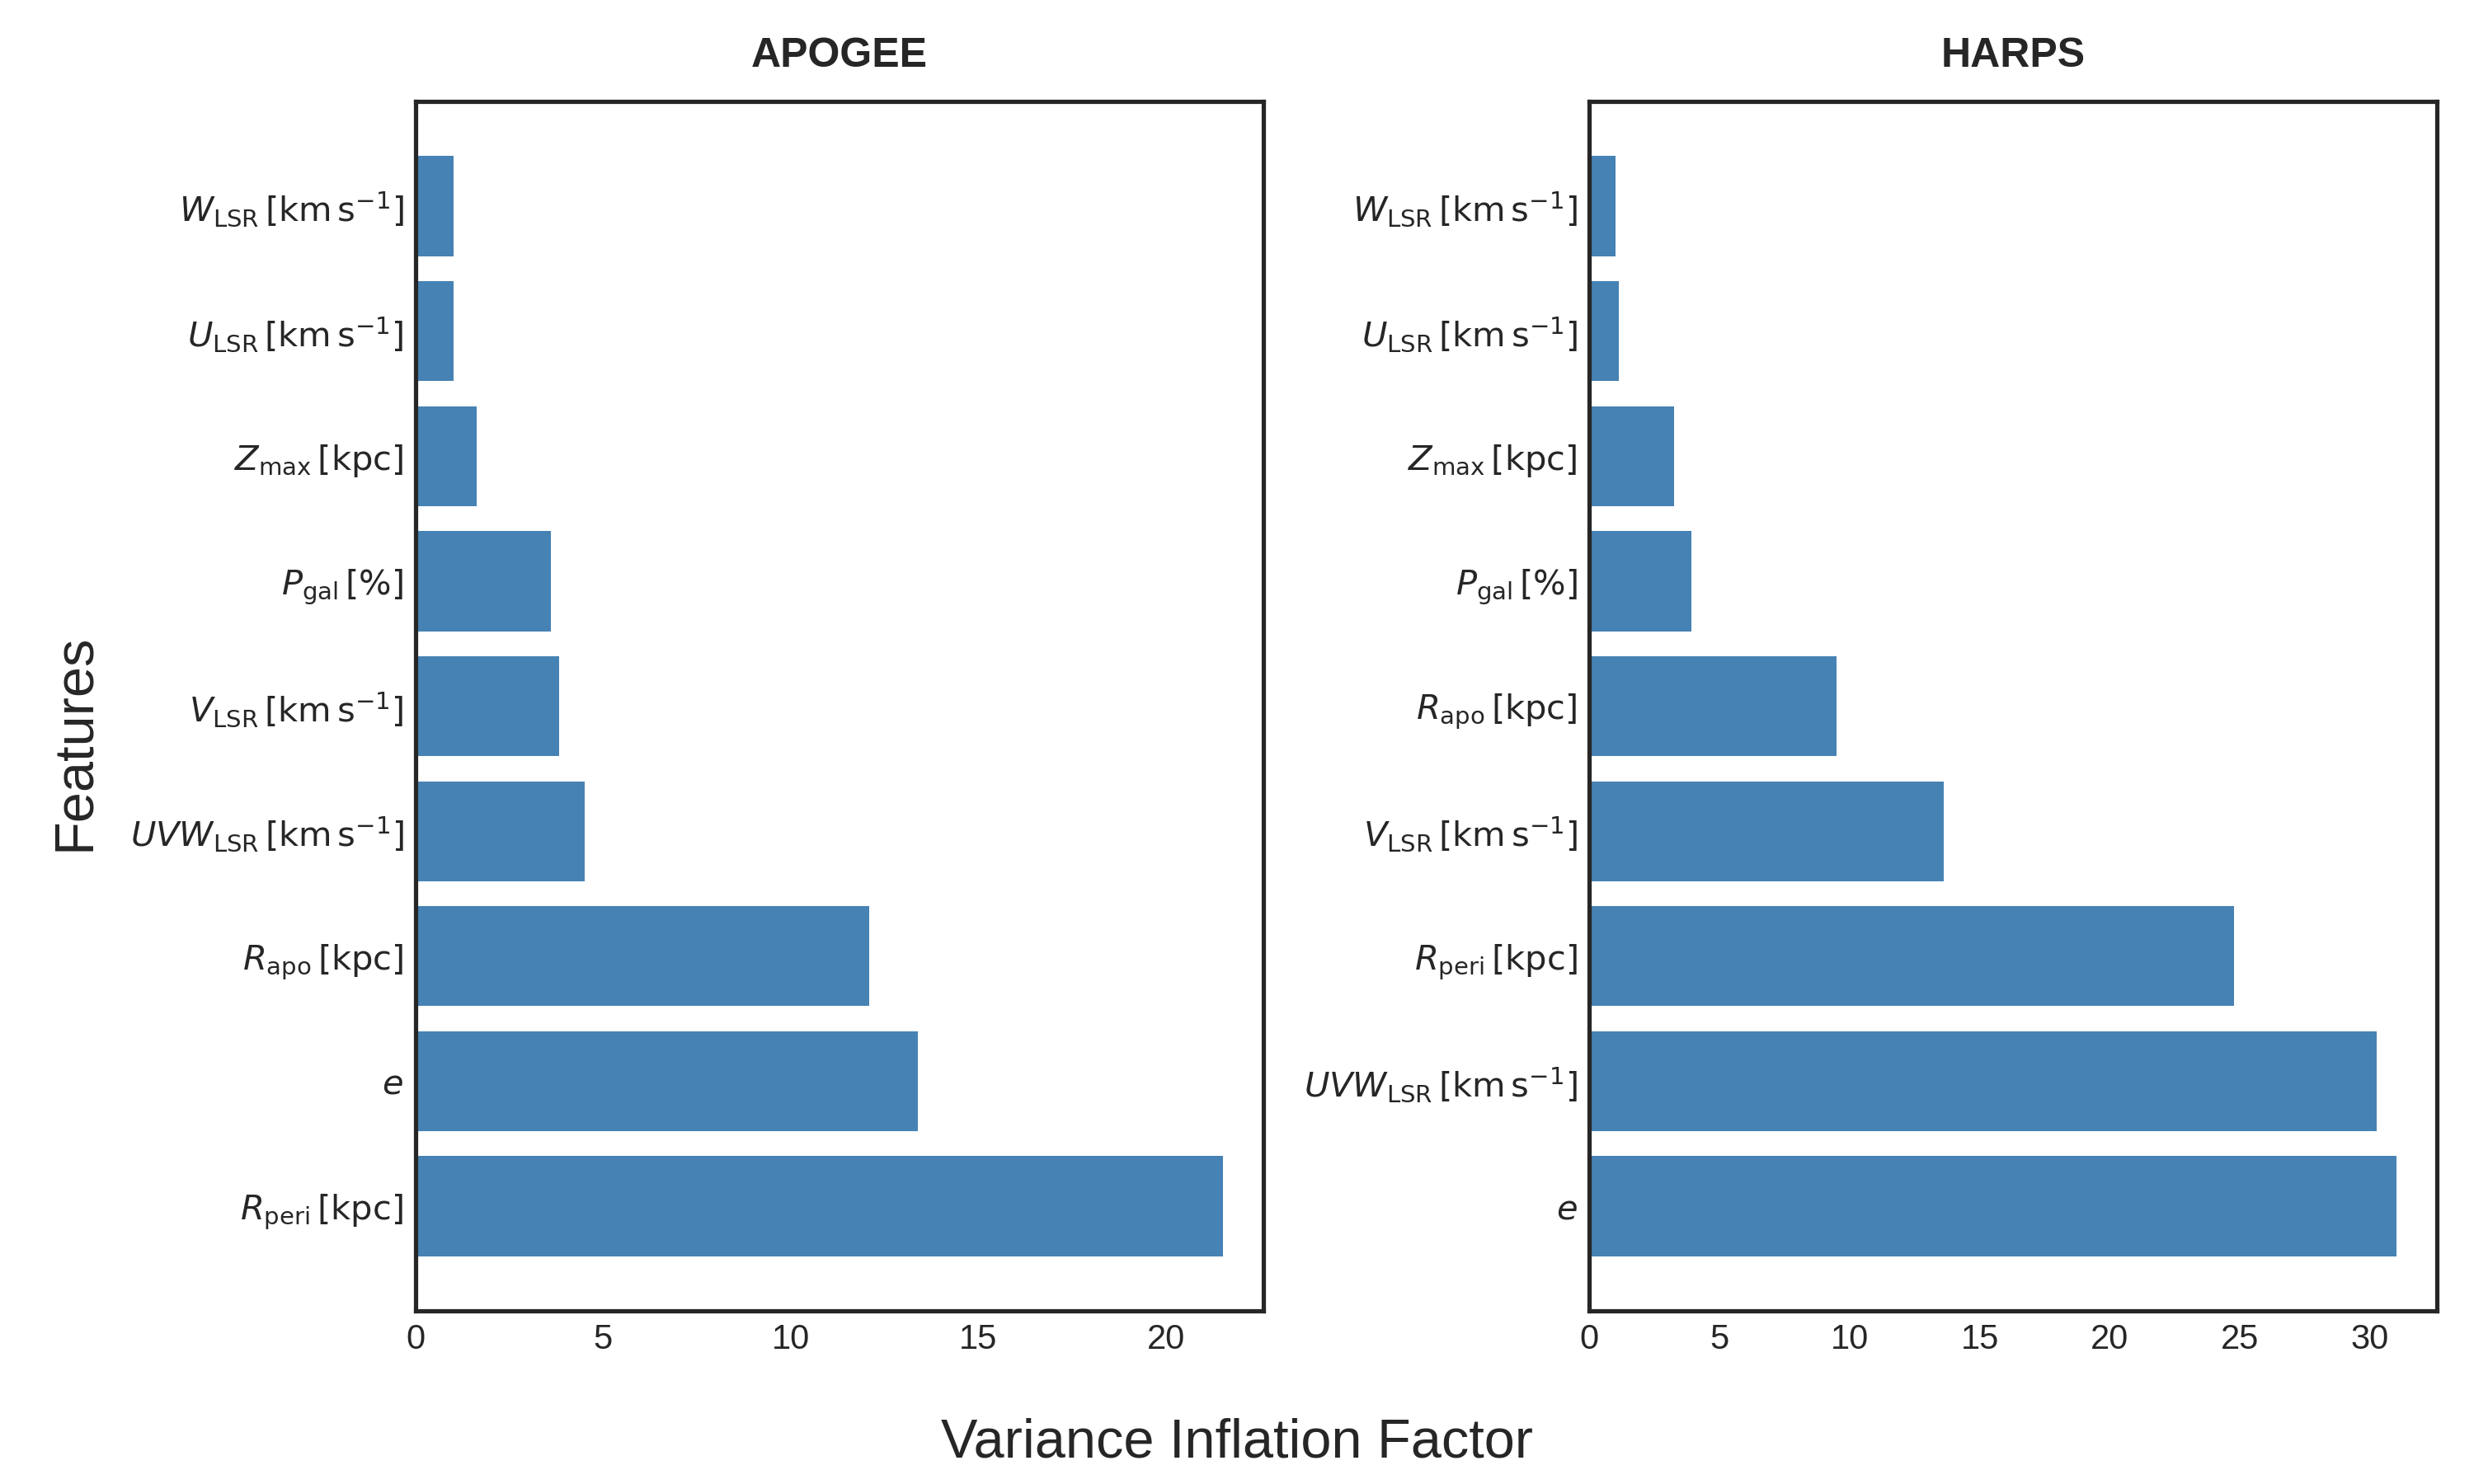
\includegraphics[width=0.49\textwidth]{VIF.png}
    \caption{Mutual information between kinematic parameters and [Fe/H] (top), and Variance inflation factors (VIF) for the kinematic parameters (bottom) in the APOGEE and HARPS samples.}
    \label{fig:mi_vif_appendix}
\end{figure}



\subsubsection{Comparison of parameter distributions}

Figure~\ref{fig:feature_distributions} presents the distributions of the kinematic and orbital parameters for the APOGEE and HARPS samples. The upper panels show probability-normalized histograms, while the lower panels display boxplots summarizing the median and spread of each parameter.

Some differences are observed between the two samples. The HARPS dataset, composed primarily of nearby solar-type dwarf stars, is confined to a relatively narrow range of velocities and orbital parameters, reflecting its local nature and selection for exoplanet surveys.
In contrast, the APOGEE red giant sample spans a significantly broader range in velocity space and orbital properties, including larger values of $Z_{\max}$, eccentricity, and total space velocity $\mathrm{UVW_{LSR}}$, consistent with its wider spatial coverage across different Galactic environments.

Despite these differences in dispersion, the APOGEE sample largely encompasses the parameter range covered by HARPS. This overlap ensures that the machine-learning models trained on APOGEE data operate within the dynamical regime relevant for the local HARPS stars, while also capturing a broader diversity of Galactic populations.

\begin{figure*}
\centering
\begin{subfigure}{0.25\textwidth}
    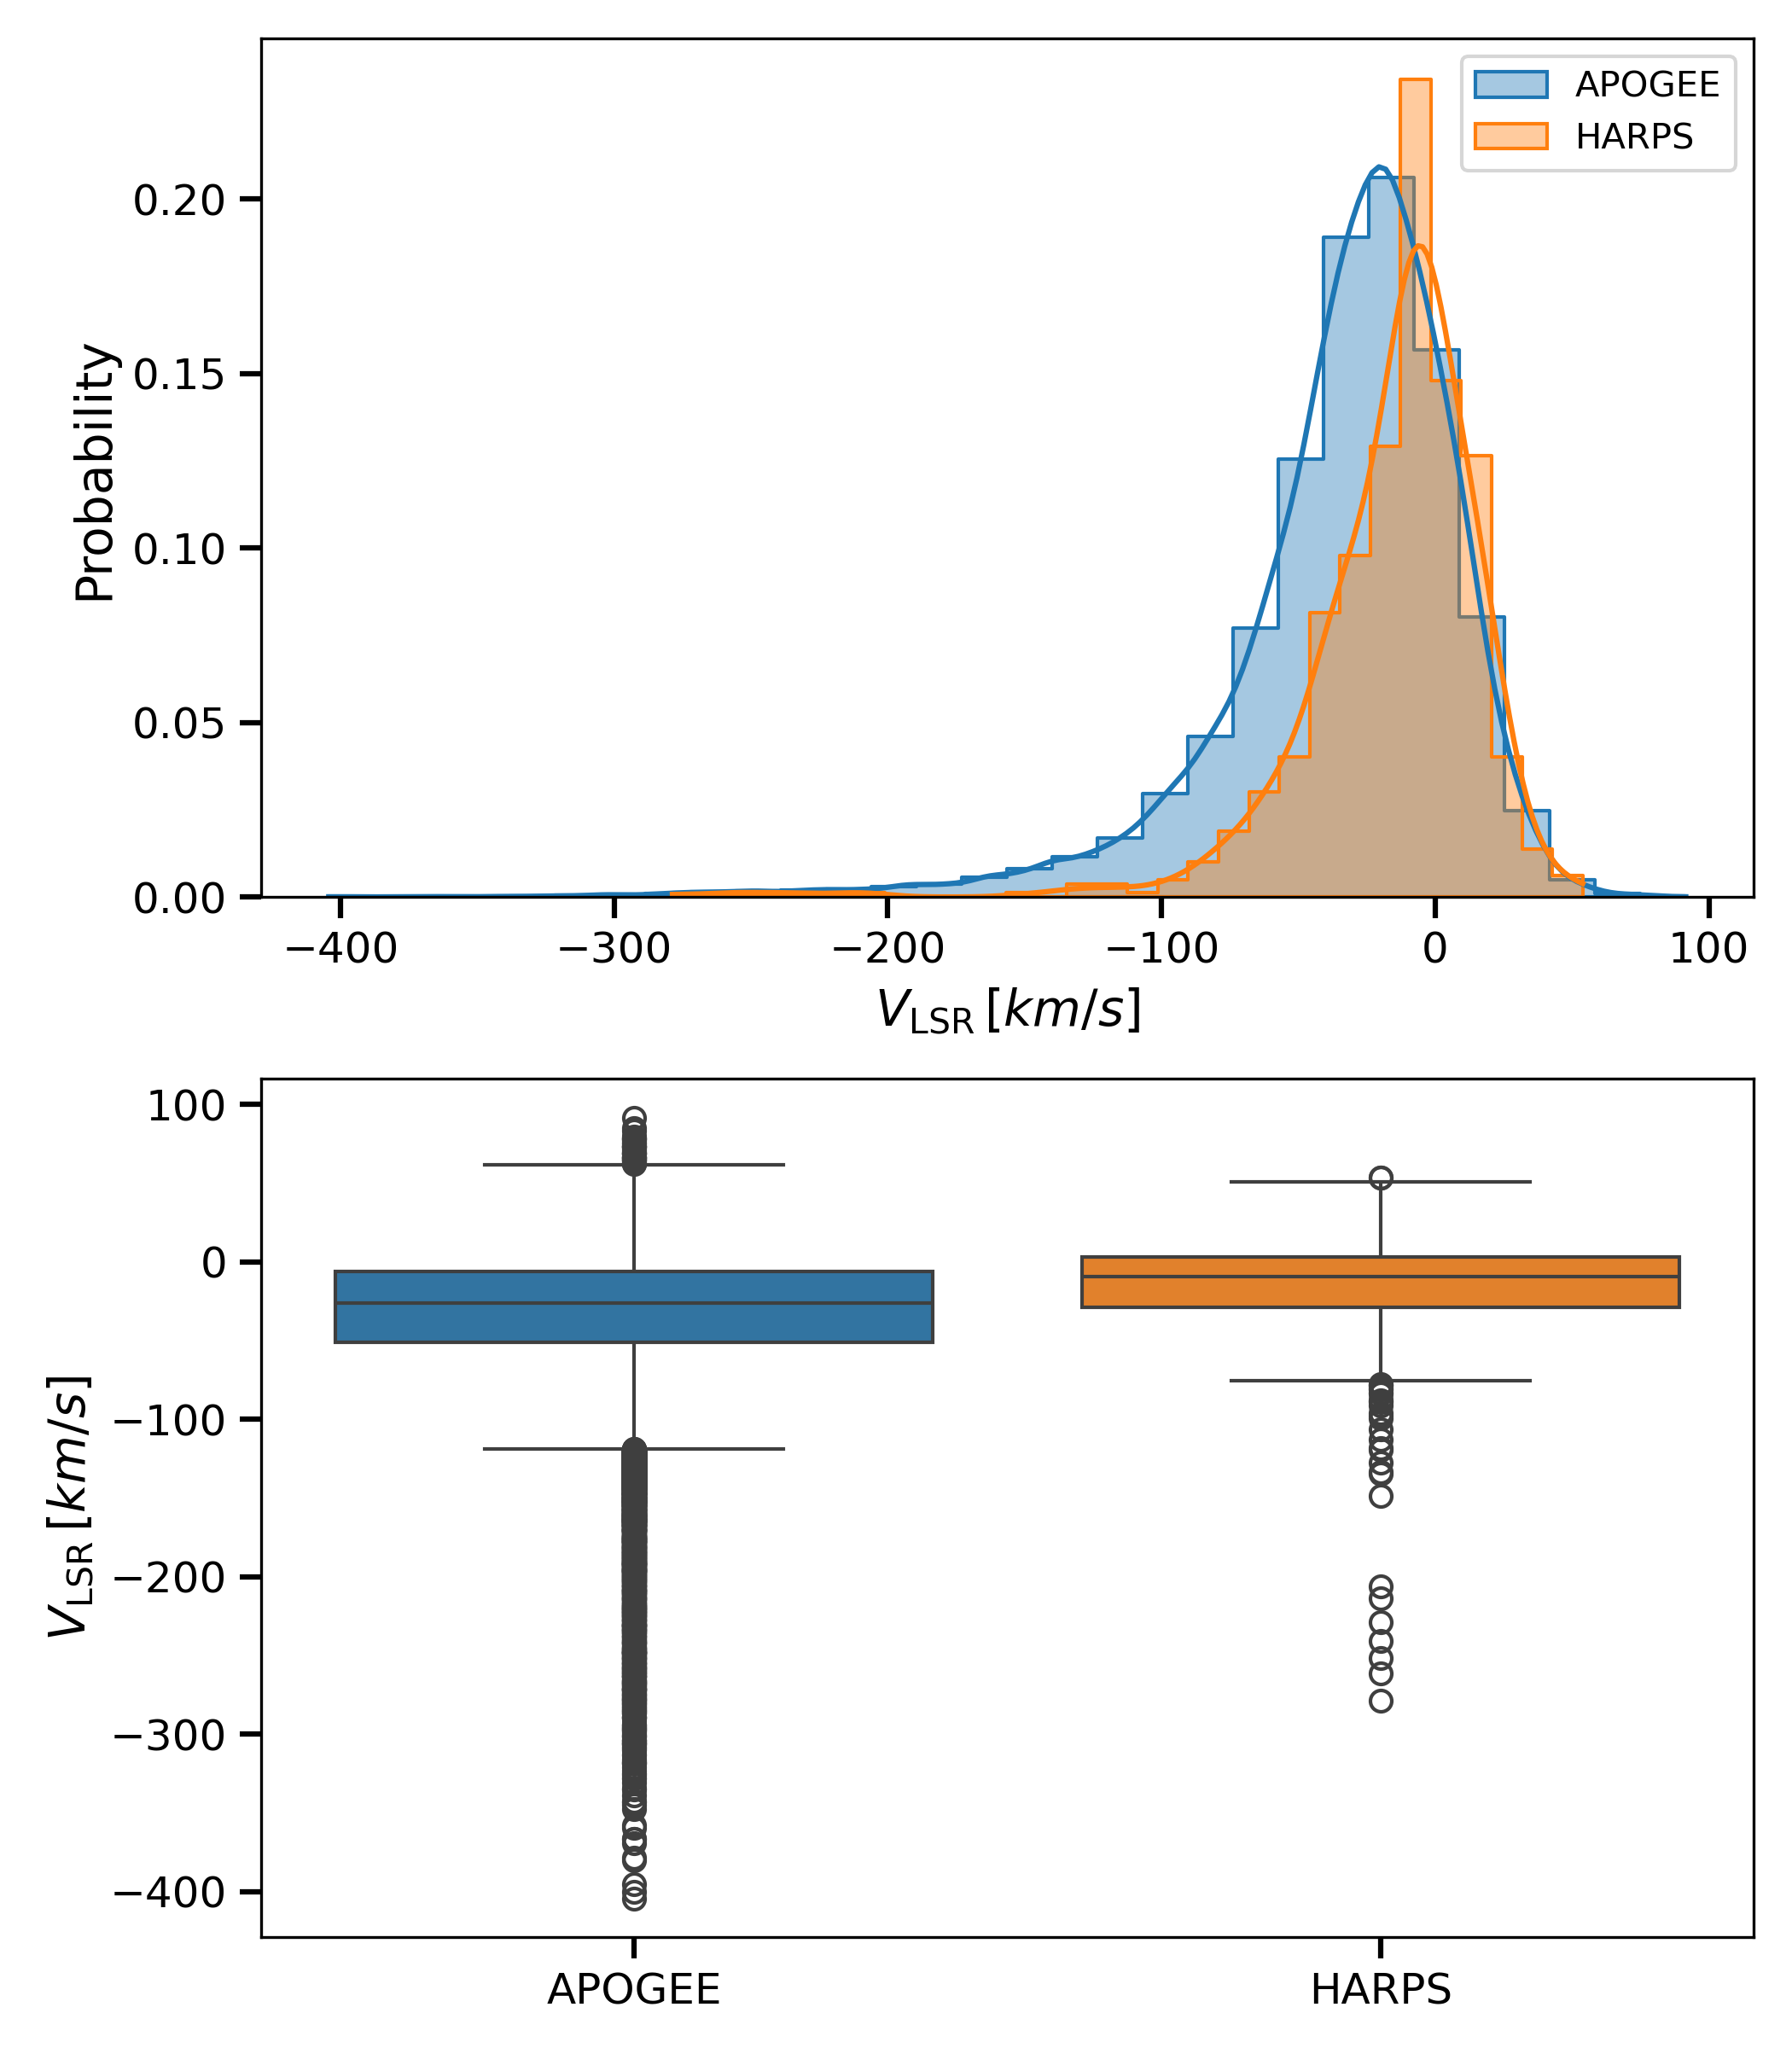
\includegraphics[width=\linewidth]{figures/dist_V_lsr.png}
    \caption{$V_{\mathrm{LSR}}\, [km/s]$}
\end{subfigure}
\begin{subfigure}{0.25\textwidth}
    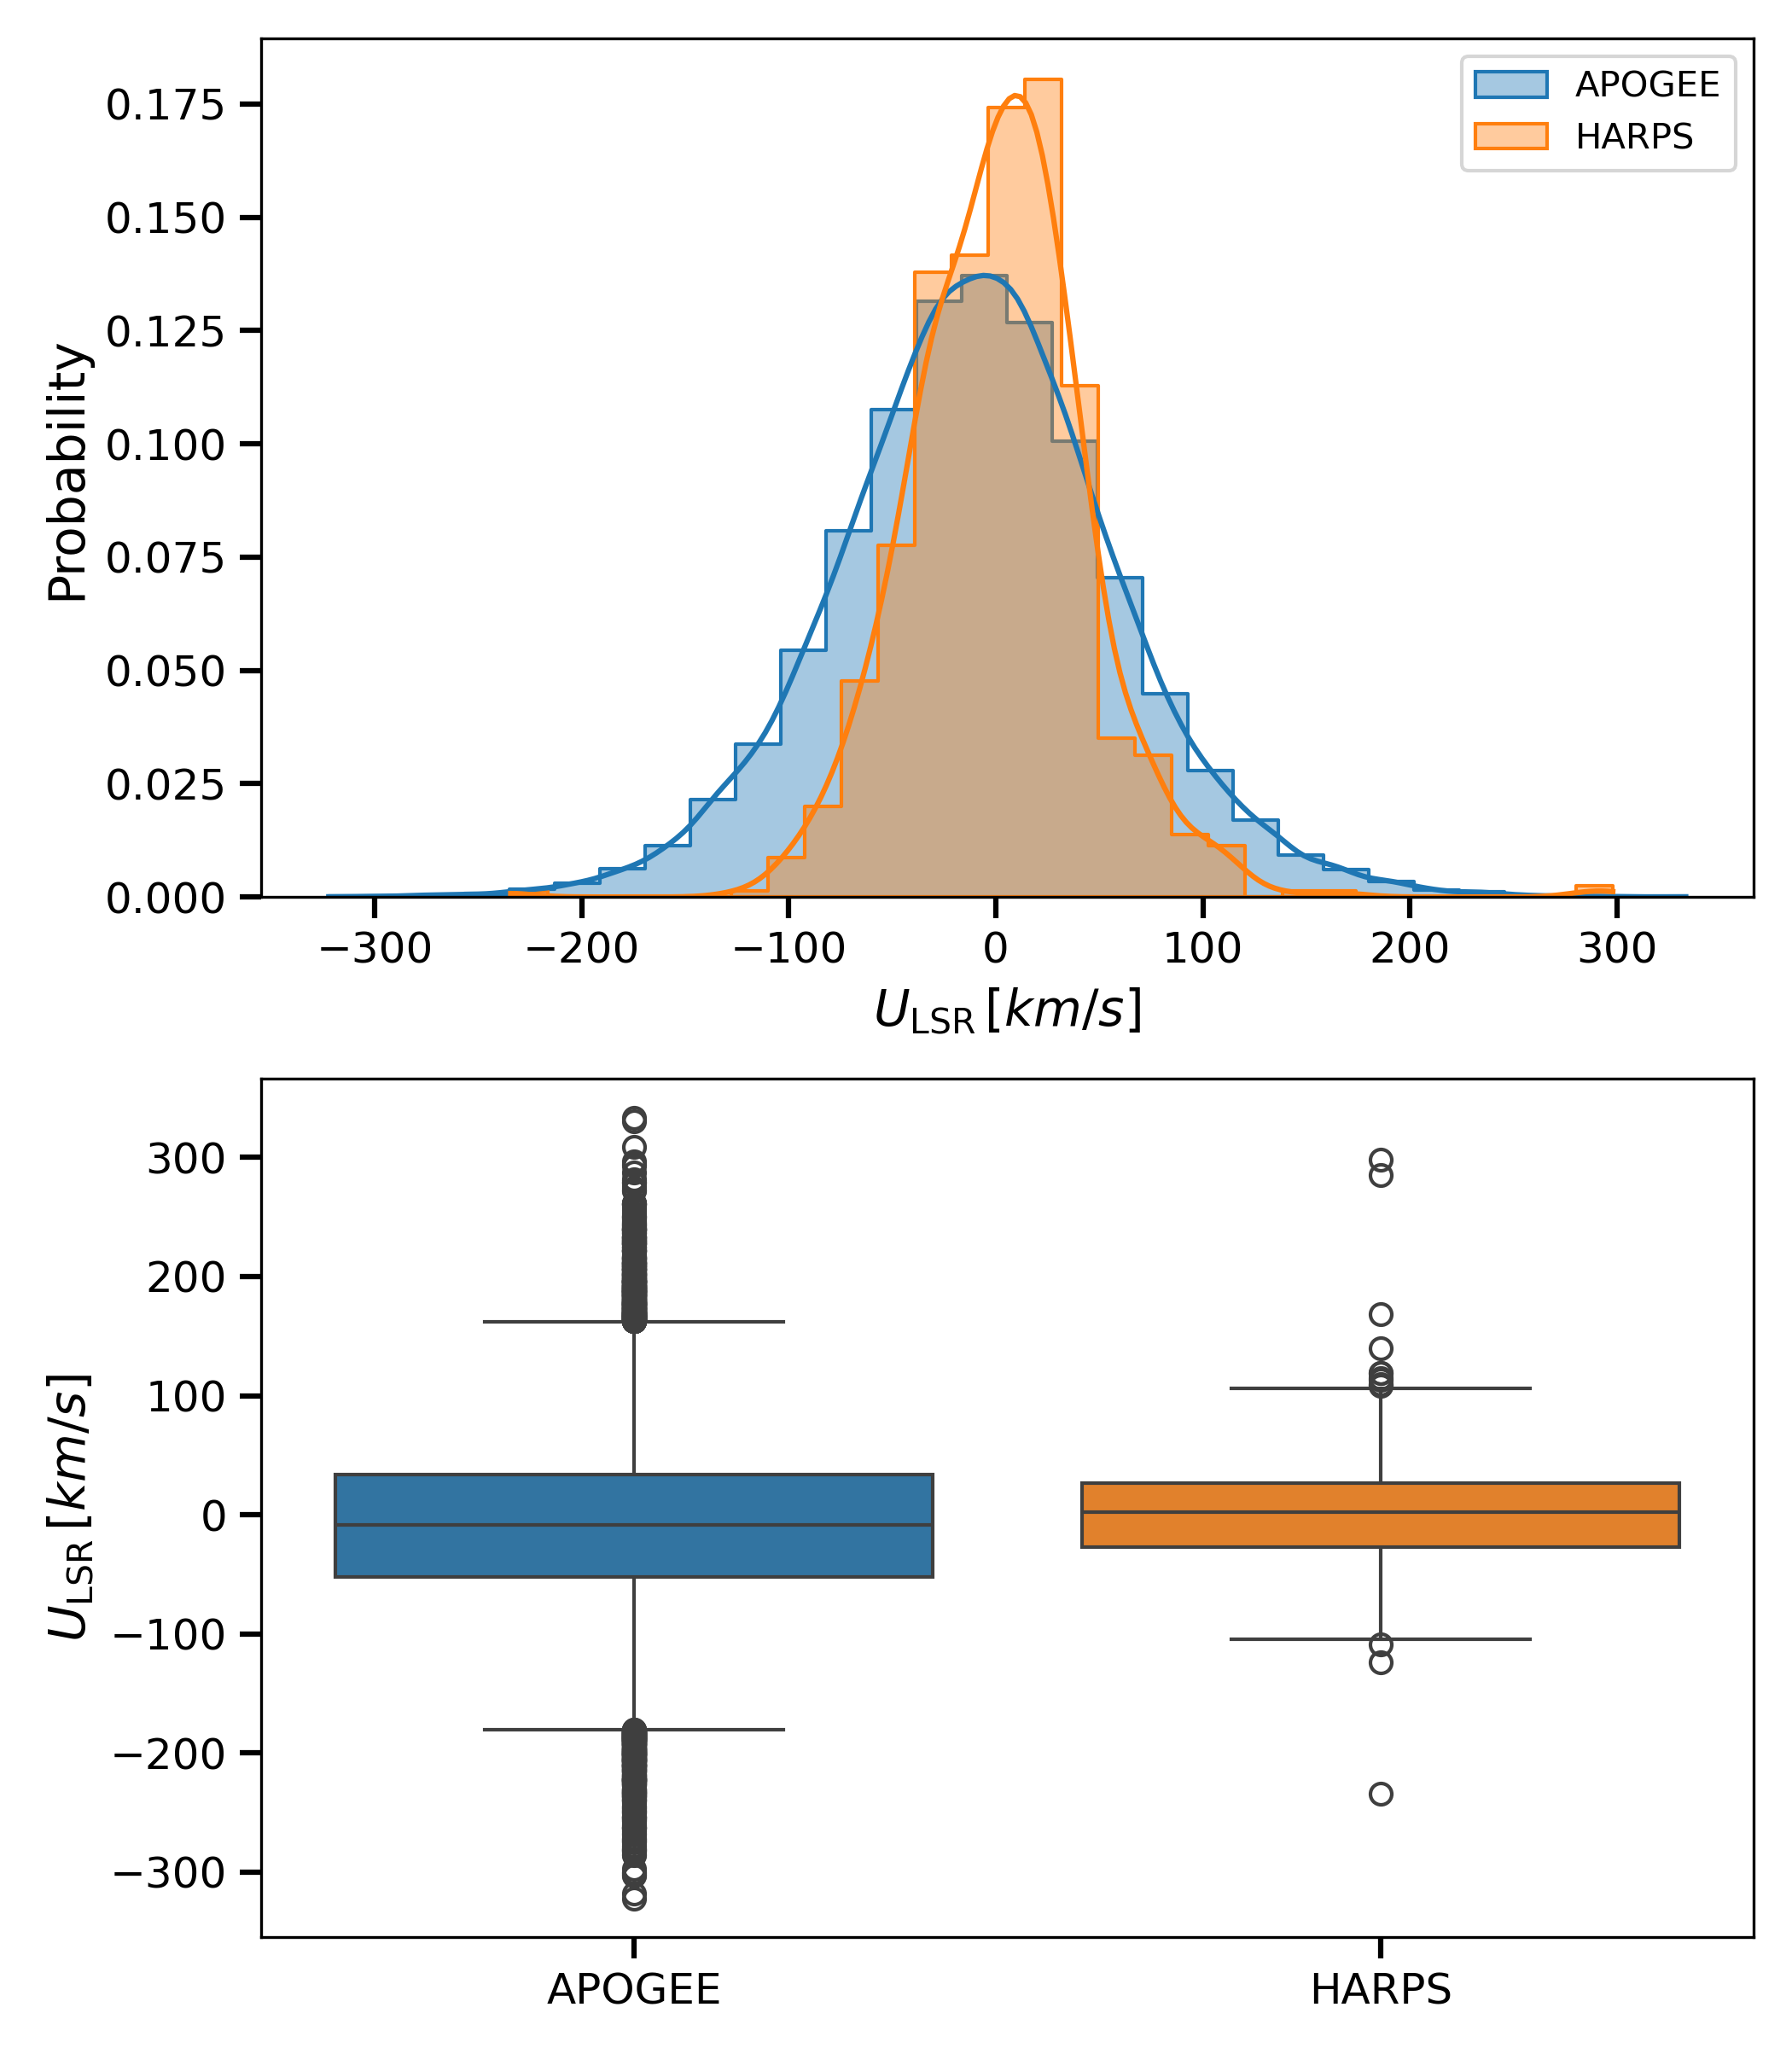
\includegraphics[width=\linewidth]{figures/dist_U_lsr.png}
    \caption{$U_{\mathrm{LSR}}\, [km/s]$}
\end{subfigure}
\begin{subfigure}{0.25\textwidth}
    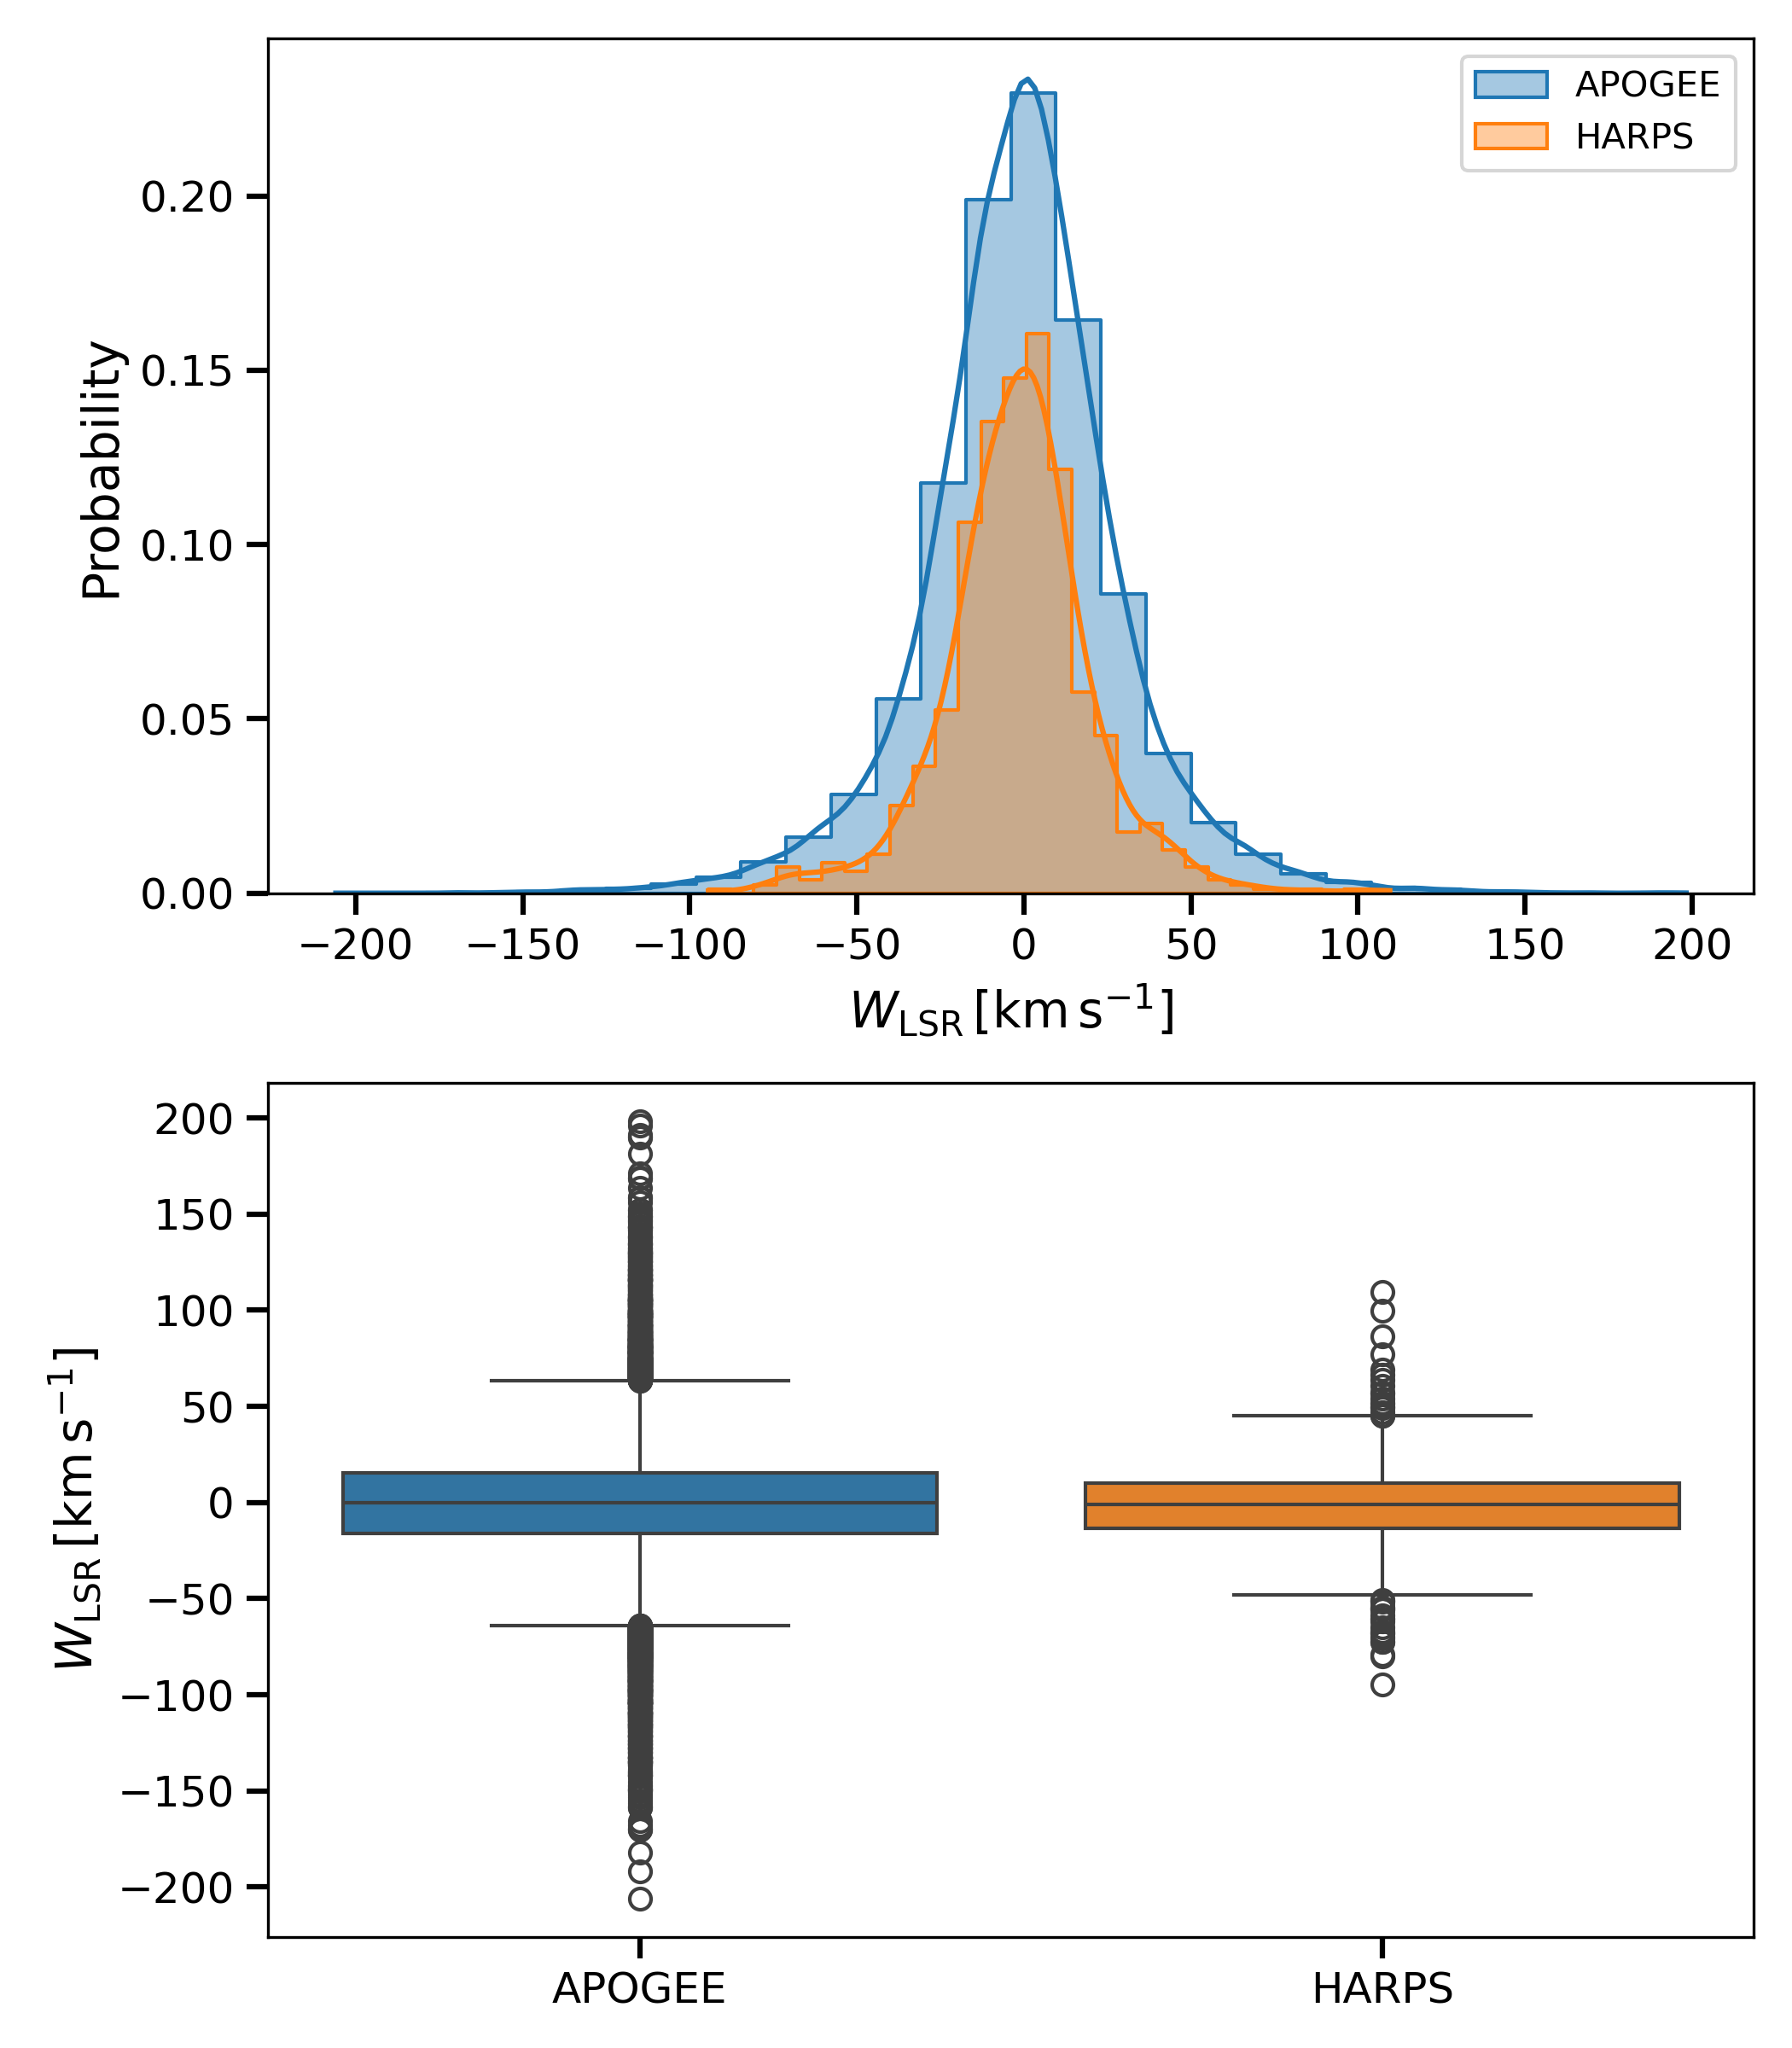
\includegraphics[width=\linewidth]{figures/dist_W_lsr.png}
    \caption{$W_{\mathrm{LSR}}\, [km/s]$}
\end{subfigure}

\vspace{0.4cm}

\begin{subfigure}{0.25\textwidth}
    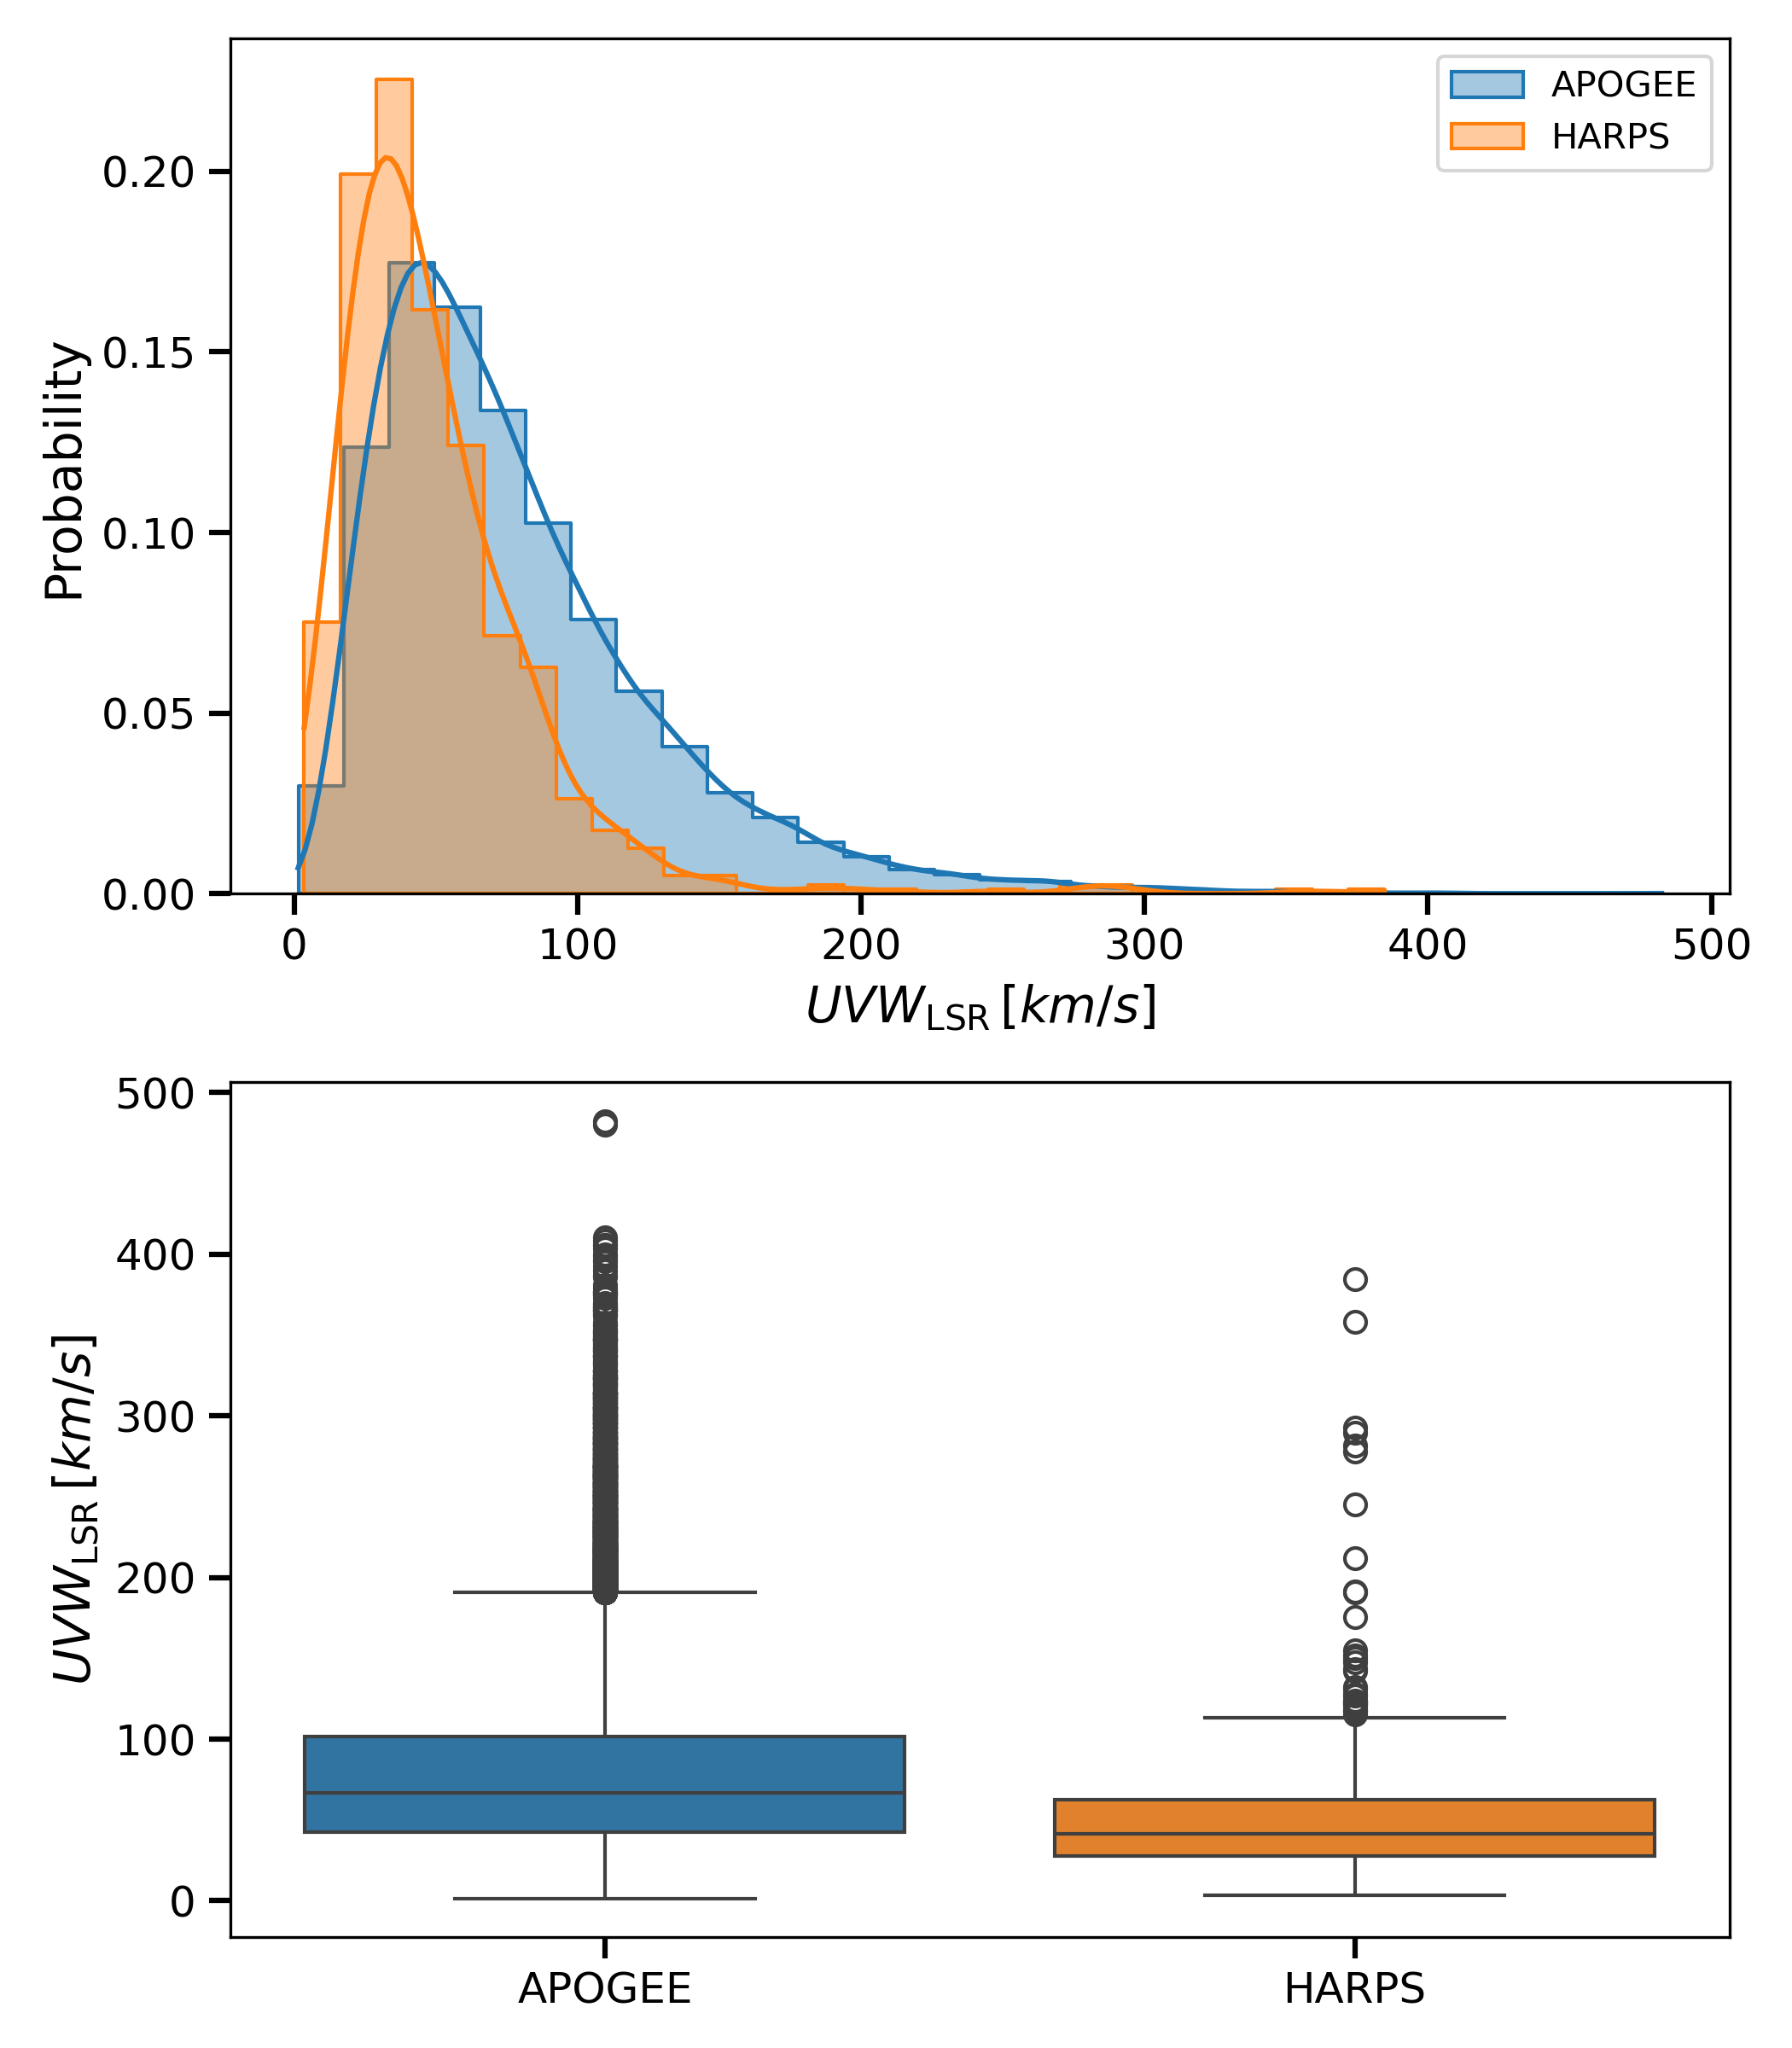
\includegraphics[width=\linewidth]{figures/dist_UVW_lsr.png}
    \caption{$UVW_{\mathrm{LSR}}\, [km/s]$}
\end{subfigure}
\begin{subfigure}{0.25\textwidth}
    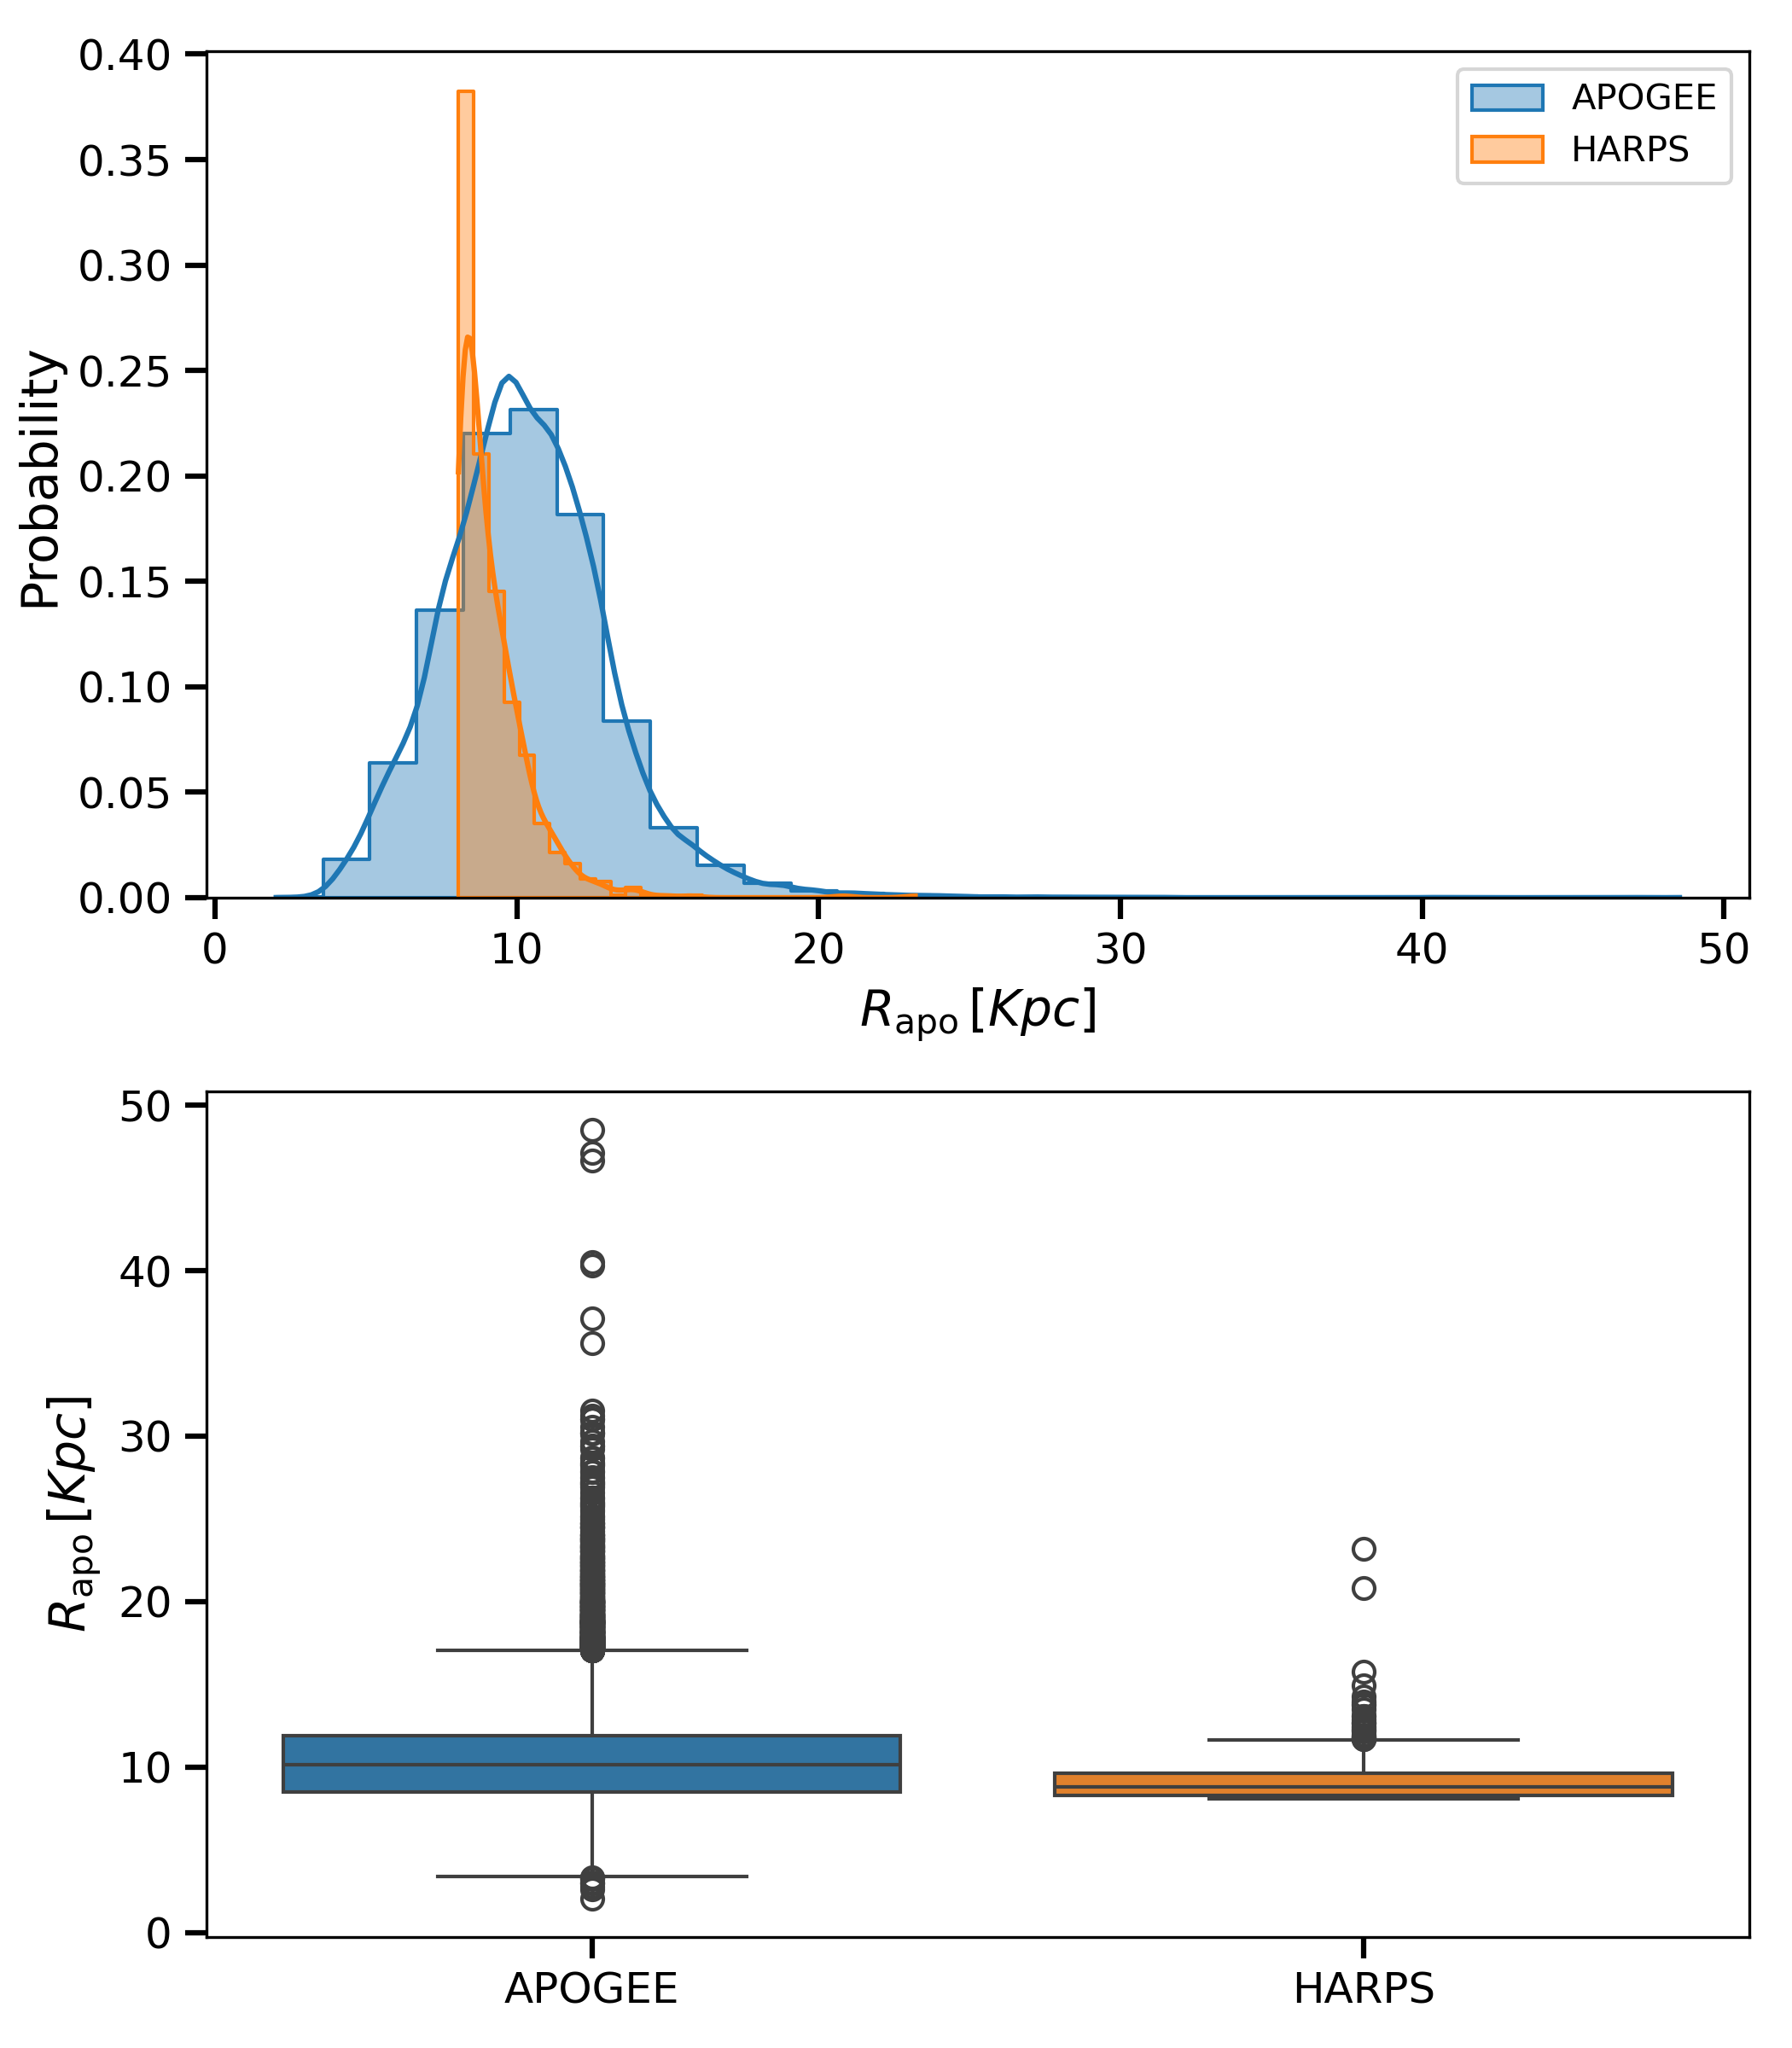
\includegraphics[width=\linewidth]{figures/dist_rapo.png}
    \caption{$R_{\mathrm{apo}}\, [Kpc]$}
\end{subfigure}
\begin{subfigure}{0.25\textwidth}
    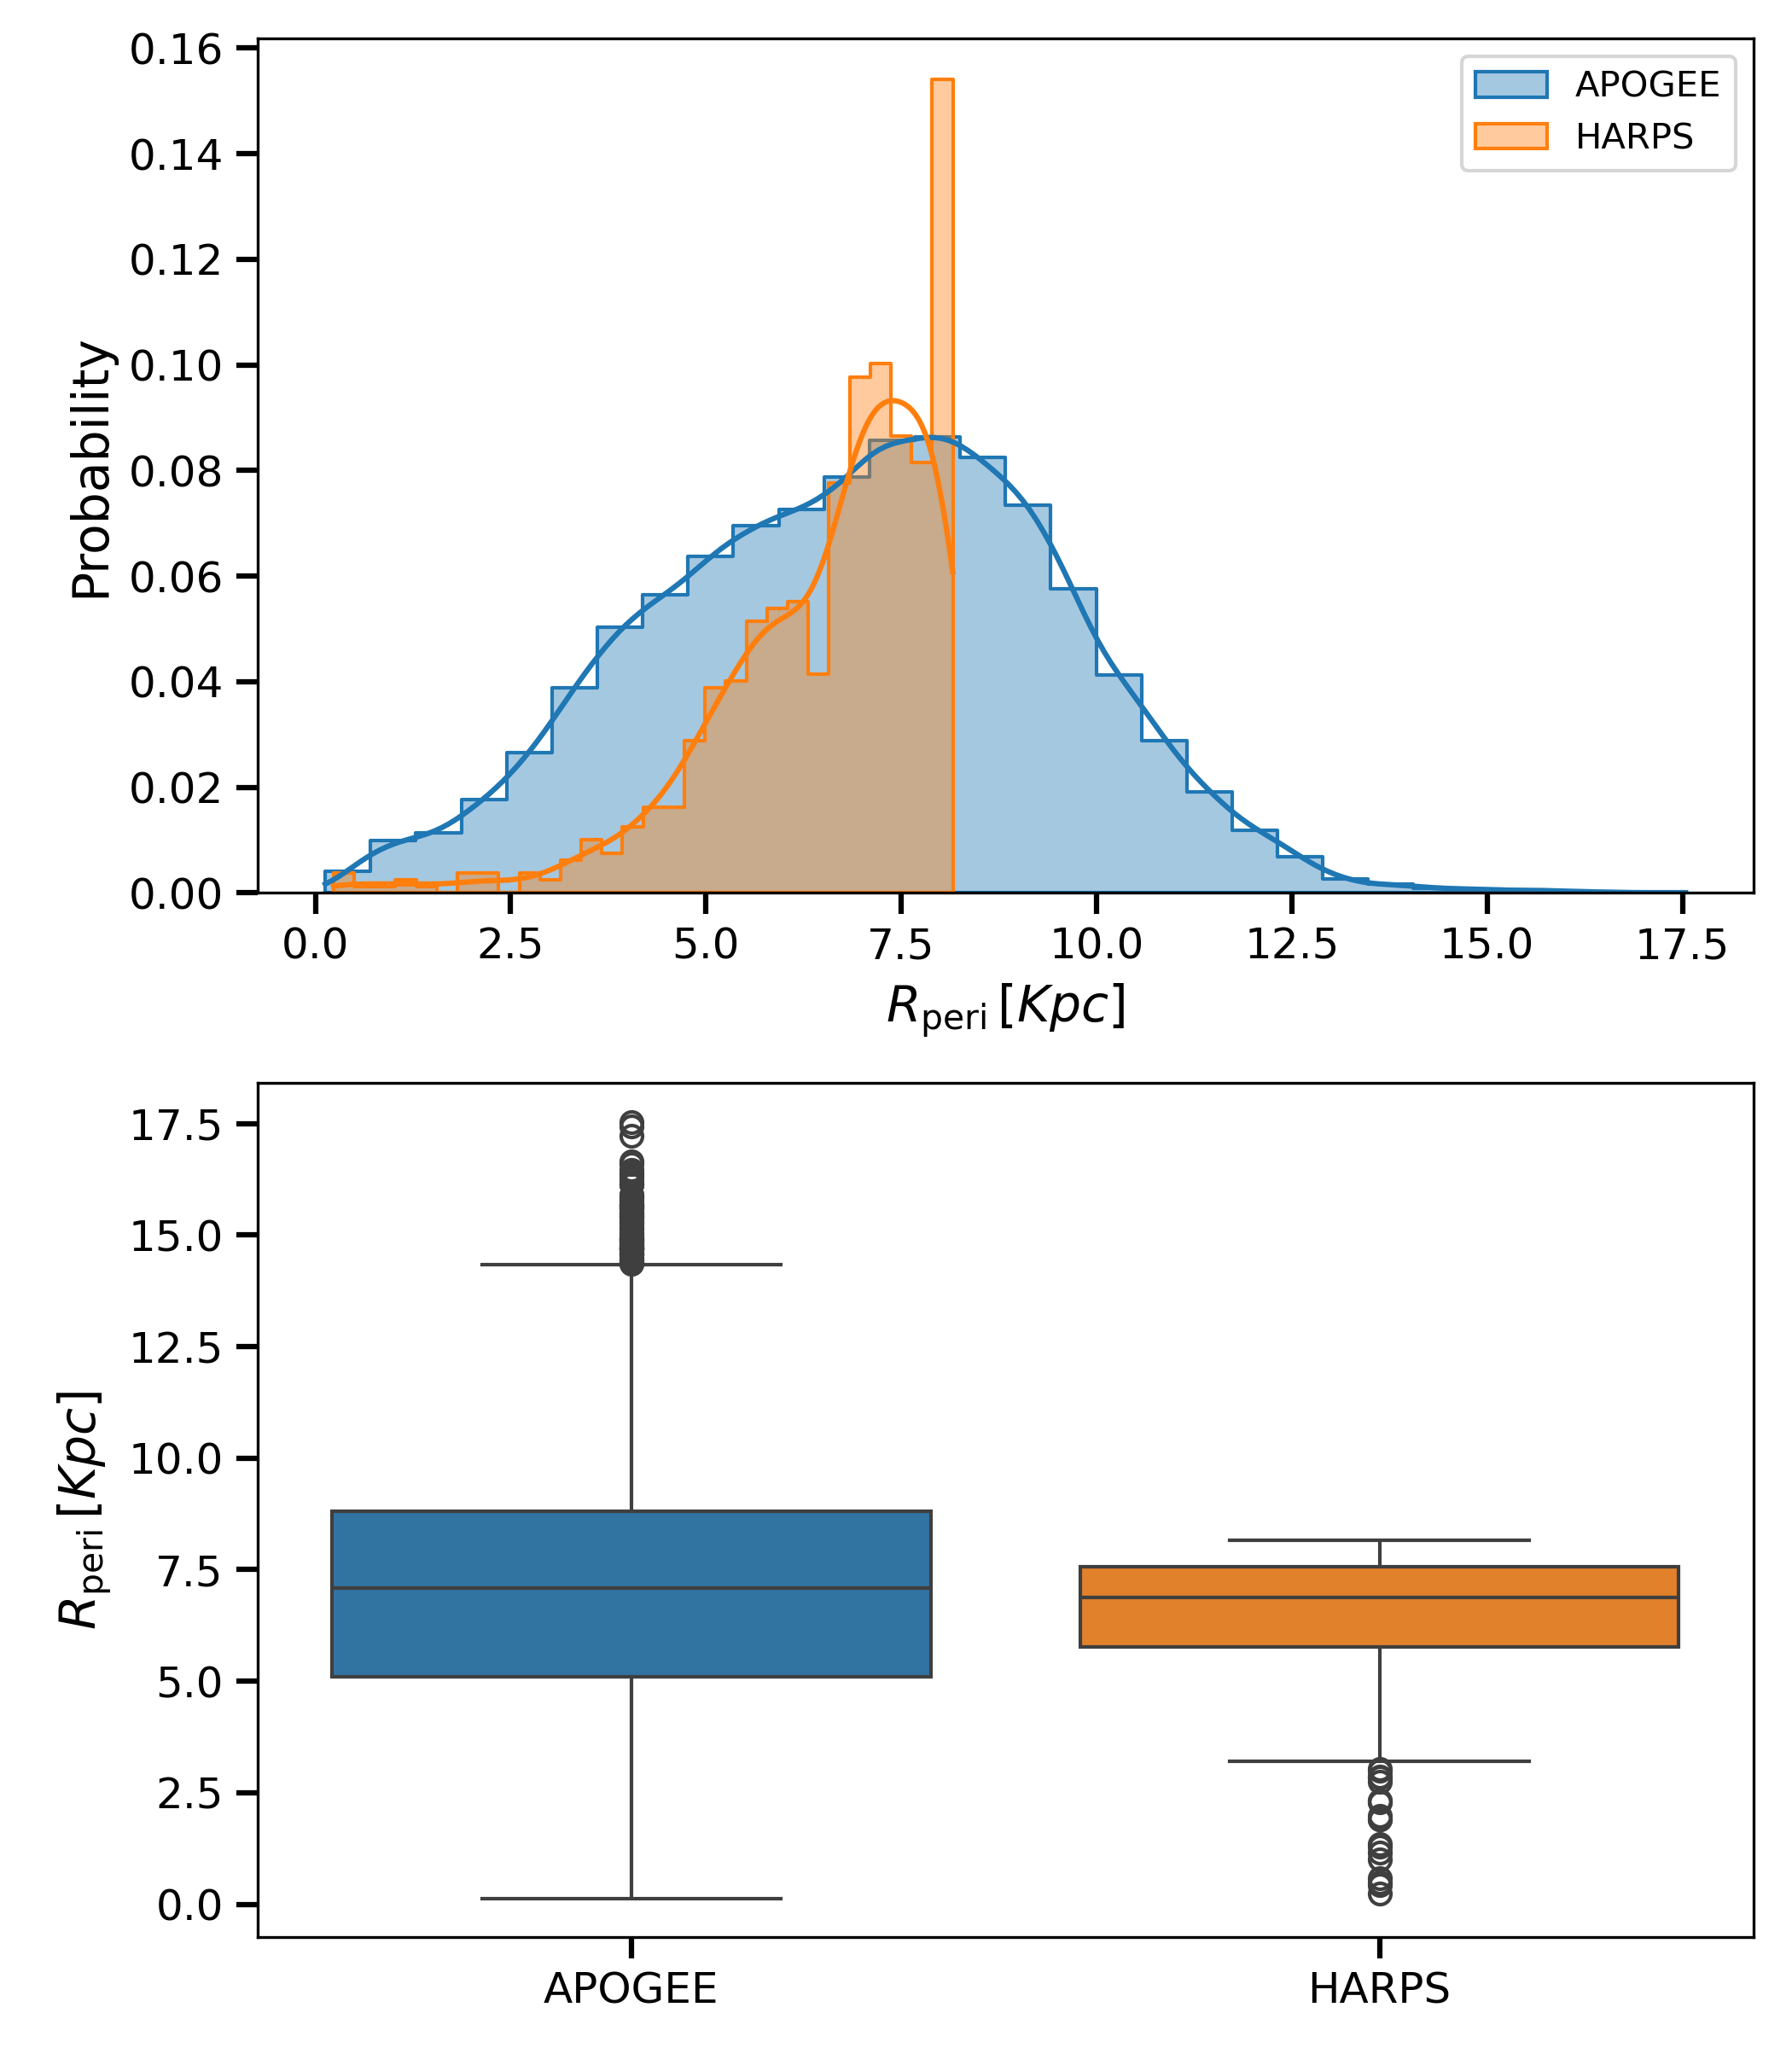
\includegraphics[width=\linewidth]{figures/dist_rperi.png}
    \caption{$R_{\mathrm{peri}}\, [Kpc]$}
\end{subfigure}

\vspace{0.4cm}

\begin{subfigure}{0.25\textwidth}
    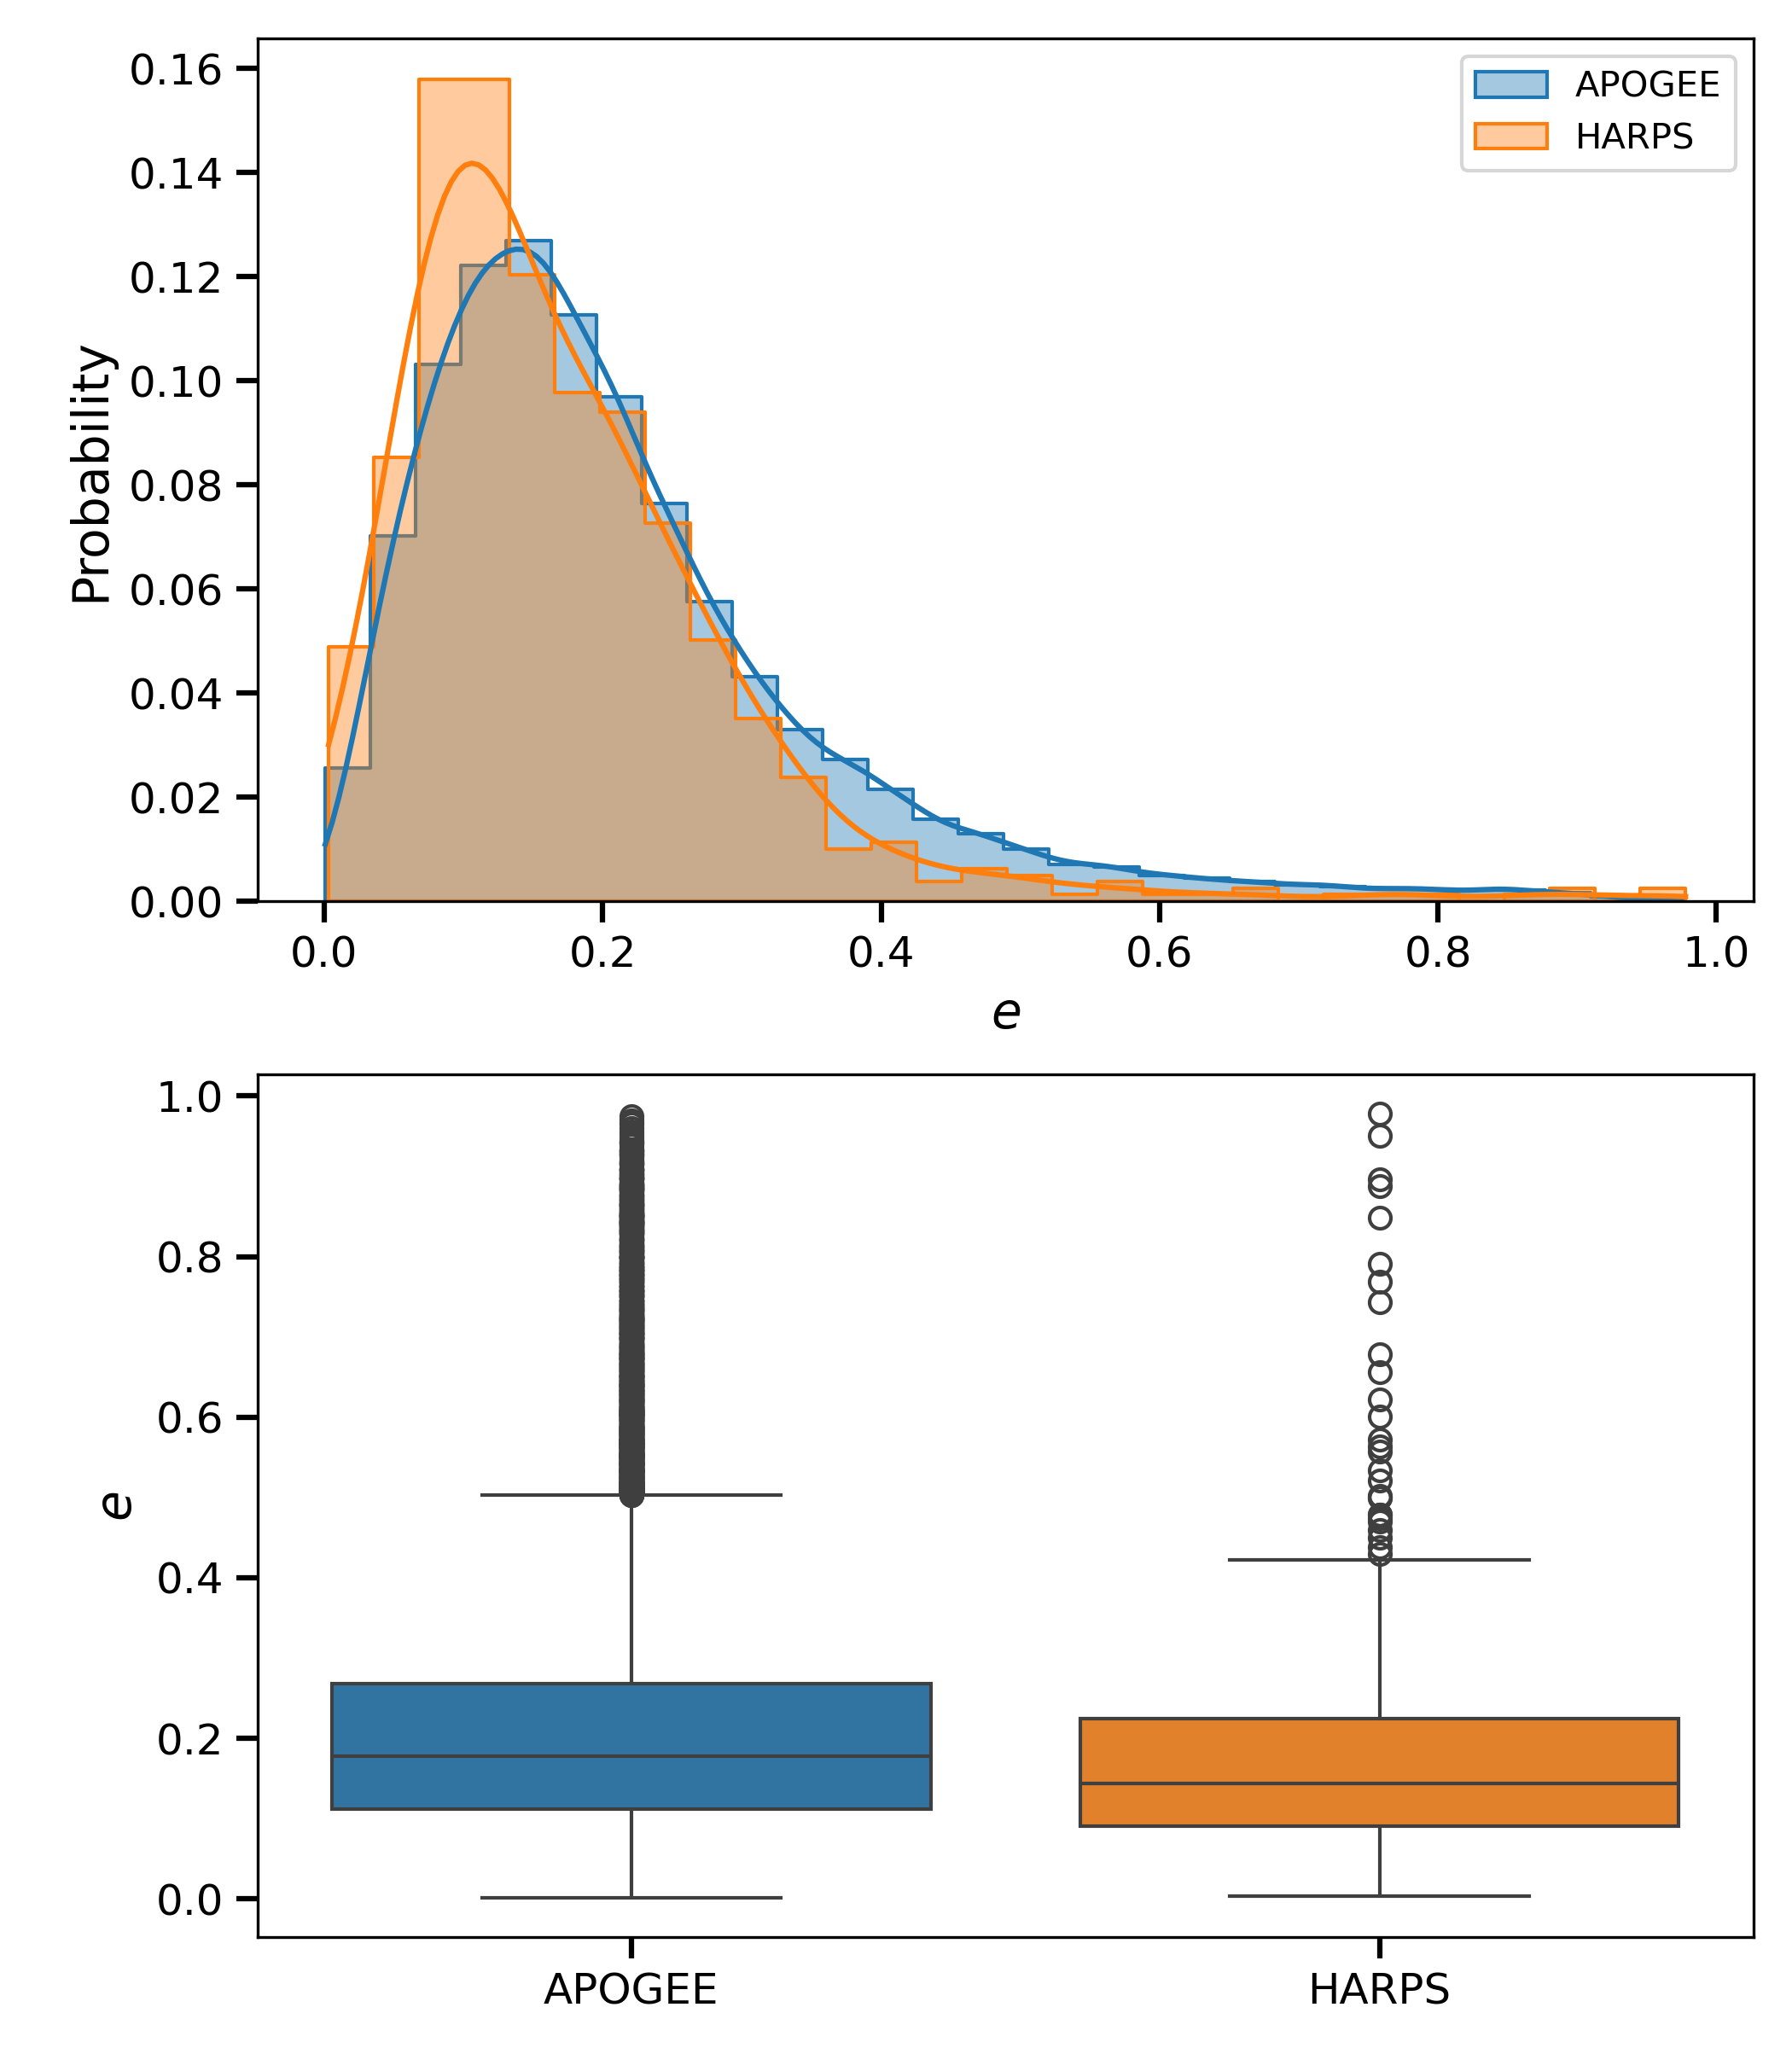
\includegraphics[width=\linewidth]{figures/dist_eccentricity.png}
    \caption{$e$}
\end{subfigure}
\begin{subfigure}{0.25\textwidth}
    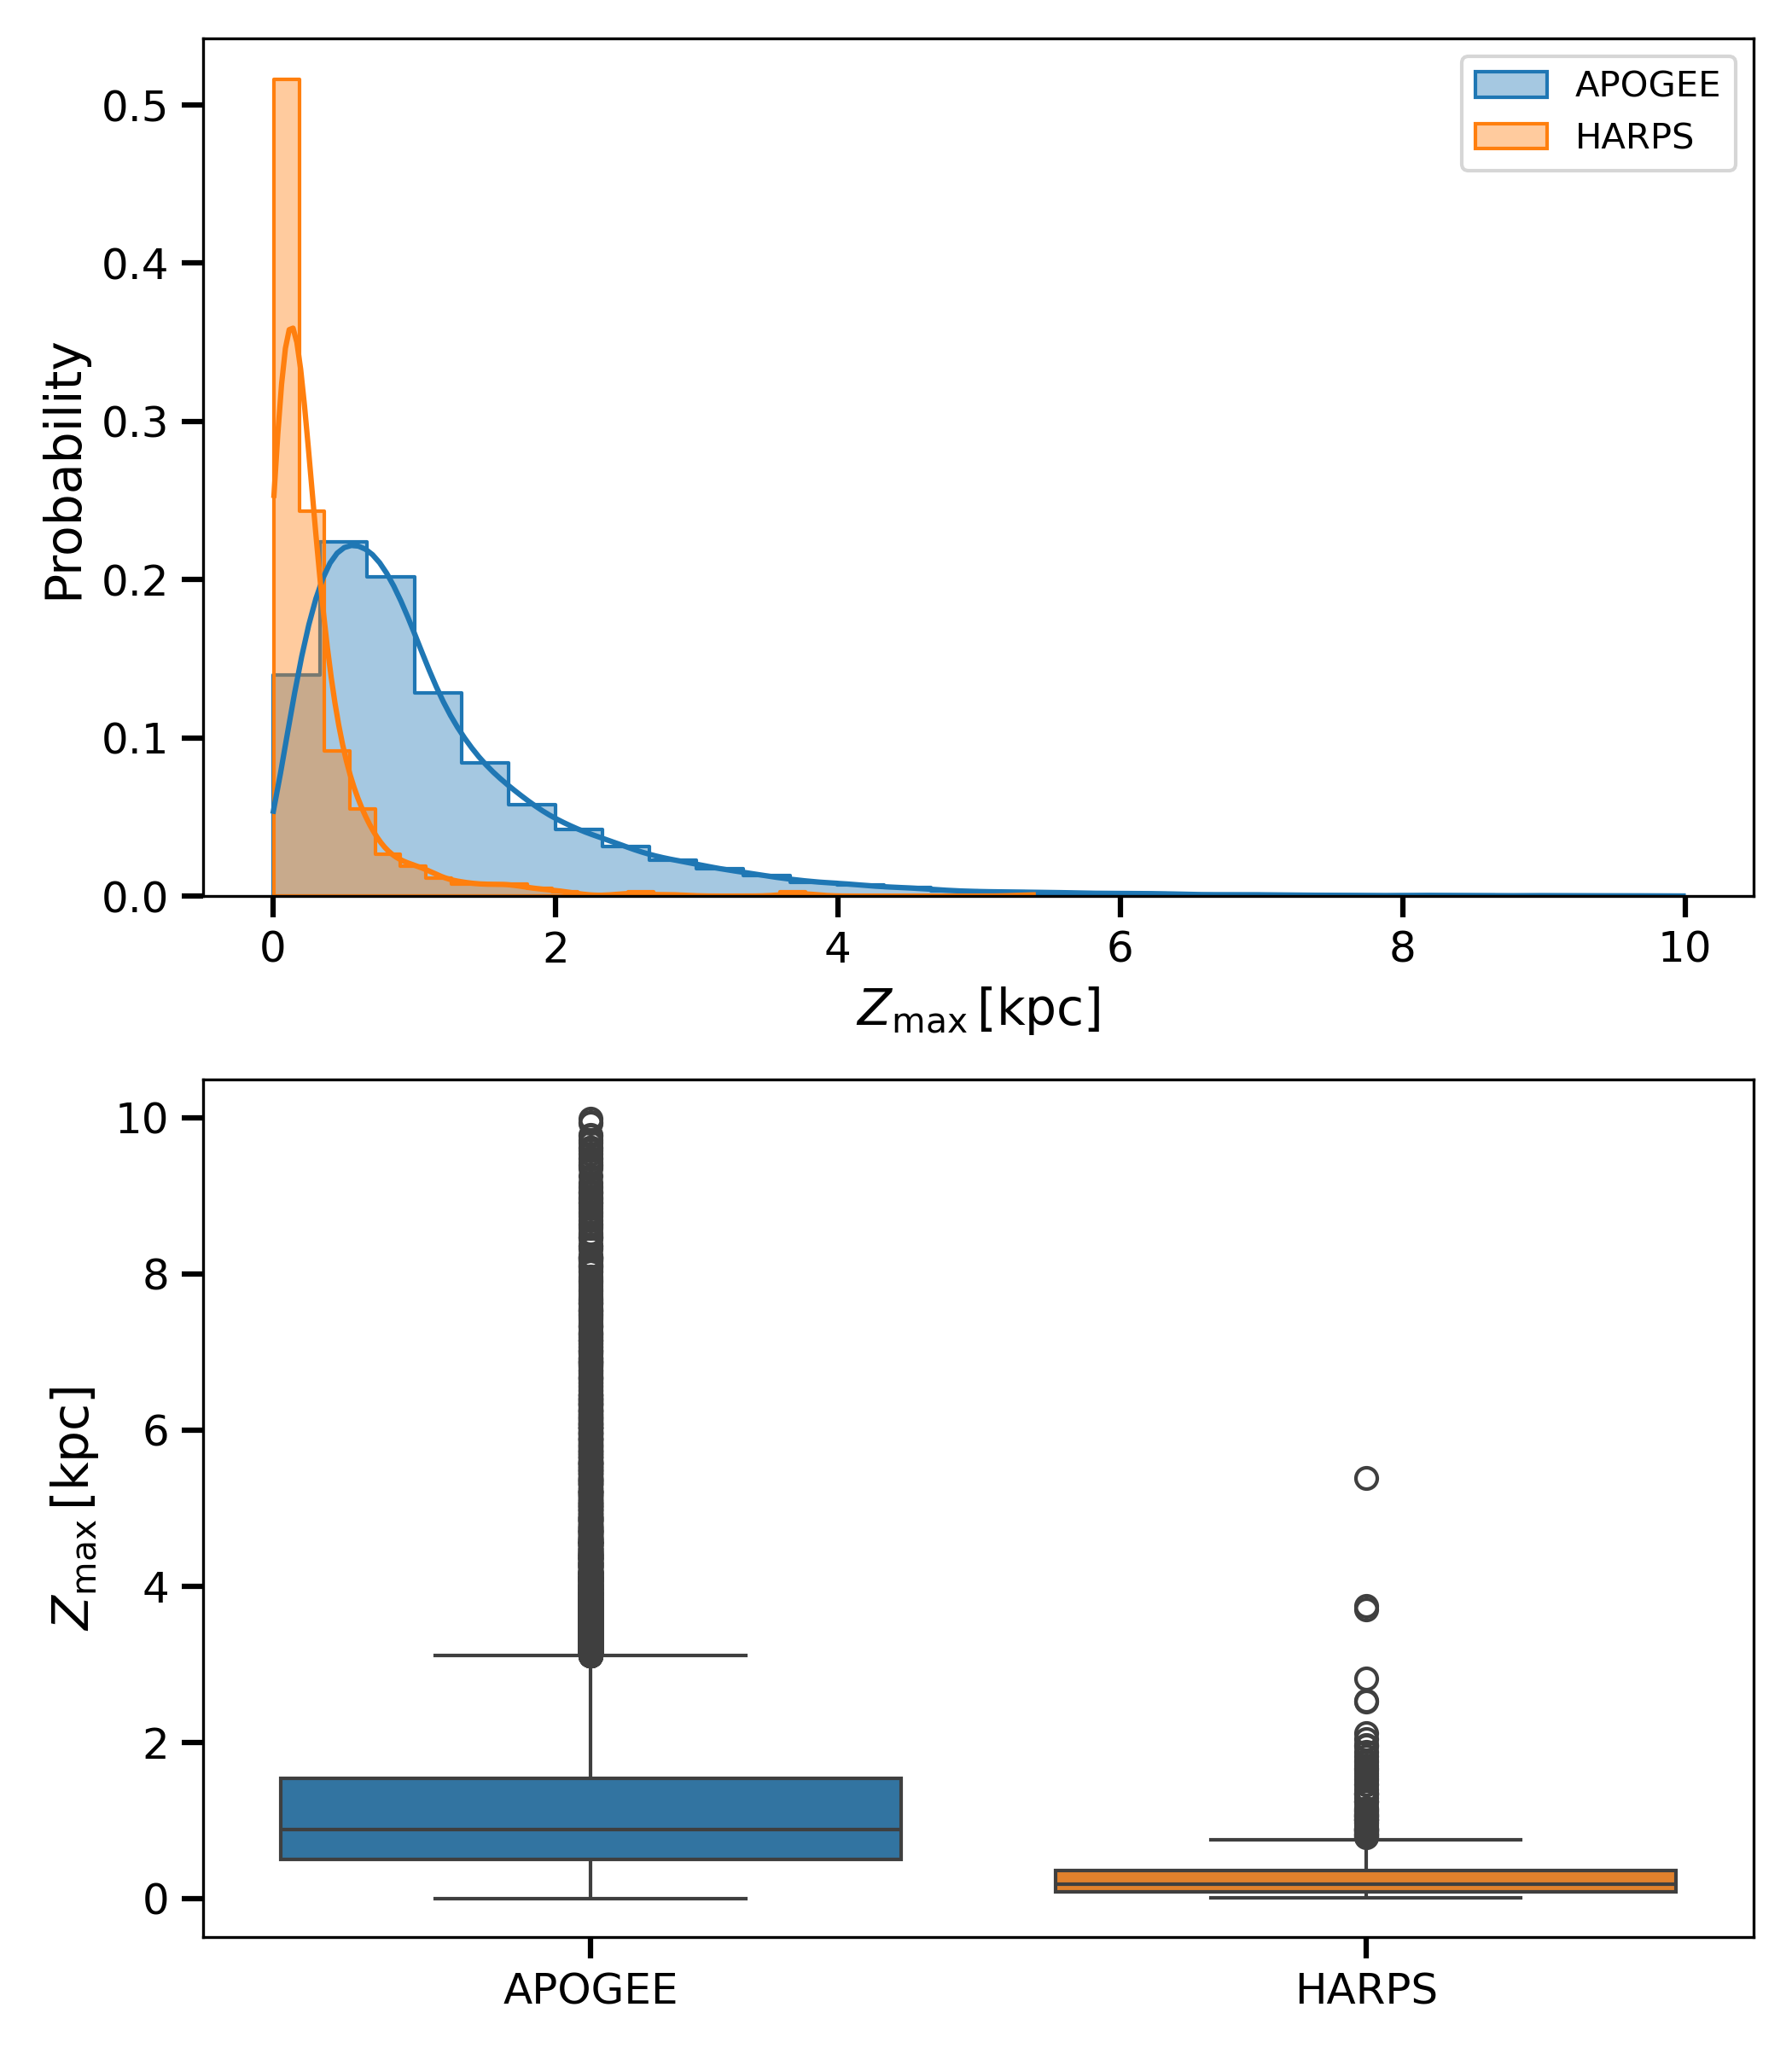
\includegraphics[width=\linewidth]{figures/dist_zmax.png}
    \caption{$Z_{\max}\, [Kpc]$}
\end{subfigure}
\begin{subfigure}{0.25\textwidth}
    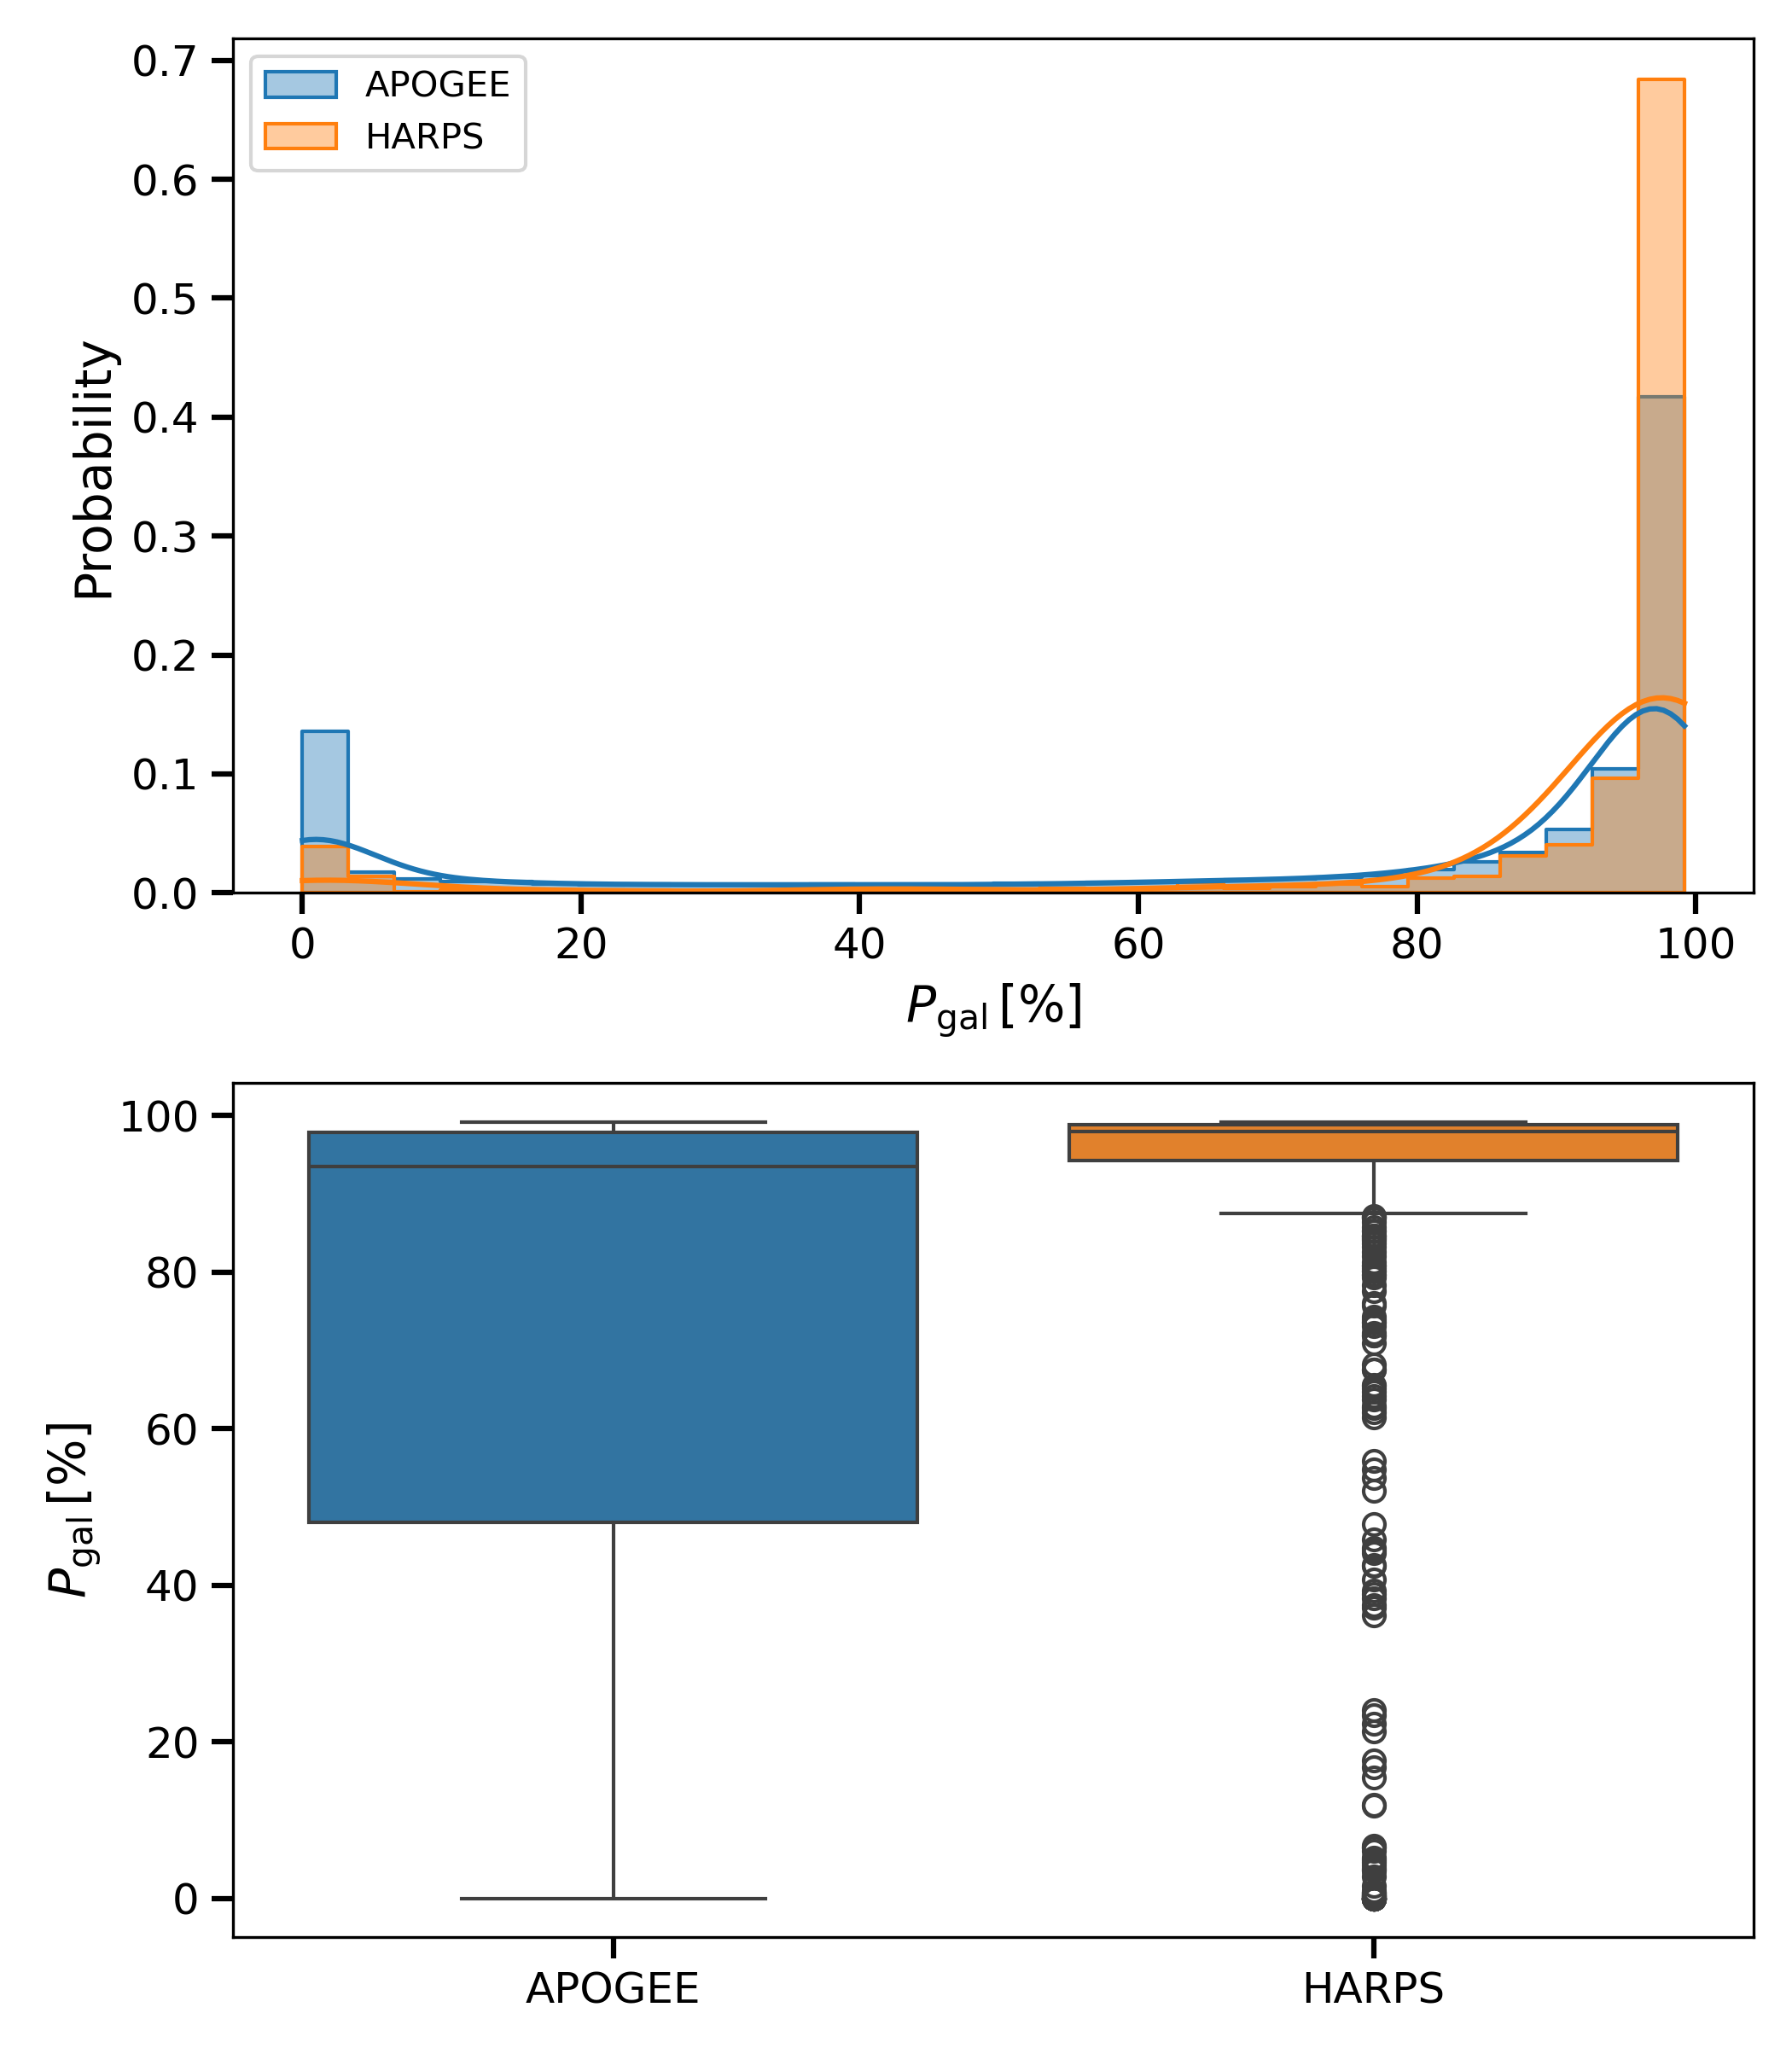
\includegraphics[width=\linewidth]{figures/dist_P_gal.png}
    \caption{$P_{\mathrm{gal}}\, [\%]$}
\end{subfigure}

\caption{Comparison of kinematic and orbital parameters distributions between the APOGEE and HARPS samples. Upper panels show probability-normalized histograms; lower panels show boxplots.}
\label{fig:feature_distributions}
\end{figure*}


\subsection{Regression benchmarks and ensemble models for [Fe/H]}

This section provides the detailed benchmarking results for the regression models used to predict stellar metallicity from kinematic parameters, together with the configuration of the ensemble methods. The goal of this analysis was to assess the intrinsic predictive power of the kinematic features under a consistent evaluation framework rather than to optimize individual algorithms.

All models were evaluated using 5-fold cross-validation with identical data splits. Performance was quantified using the root mean squared error (RMSE), mean absolute error (MAE), and coefficient of determination ($R^2$). Table~\ref{tab:cv_scores_full} summarizes the mean performance across folds, with the quoted RMSE uncertainties corresponding to the standard deviation over folds. The small standard deviations of the RMSE across folds indicate stable model performance.

\begin{table}
\caption{Performance of regression models evaluated using 5-fold cross-validation.
Reported values correspond to the mean across folds, with RMSE uncertainties
indicating the standard deviation.}
\centering
\begin{tabular}{lccc}
\hline
Model & RMSE (dex) & MAE (dex) & $R^2$ \\
\hline
Linear Regression & $0.213 \pm 0.001$ & 0.169 & 0.329 \\
Random Forest & $0.203 \pm 0.001$ & 0.159 & 0.391 \\
Extra Trees & $0.204 \pm 0.001$ & 0.160 & 0.384 \\
XGBoost & $0.204 \pm 0.001$ & 0.160 & 0.386 \\
XGBoost (QT) & $0.204 \pm 0.001$ & 0.160 & 0.386 \\
LightGBM & $\mathbf{0.199 \pm 0.001}$ & 0.156 & 0.412 \\
LightGBM (QT) & $0.199 \pm 0.001$ & 0.156 & 0.412 \\
CatBoost & $0.200 \pm 0.001$ & 0.157 & 0.411 \\
CatBoost (QT) & $0.200 \pm 0.001$ & 0.156 & 0.408 \\
Voting Regressor & $0.200 \pm 0.001$ & 0.157 & 0.410 \\
Stacking Regressor & $0.199 \pm 0.001$ & 0.156 & 0.413 \\
\hline
\end{tabular}
\label{tab:cv_scores_full}
\end{table}


We also considered target ([Fe/H]) transformation using a quantile normalization (QT), which maps the metallicity distribution onto a Gaussian form via its empirical cumulative distribution function, but it did not improve predictive accuracy. This is consistent with the approximately symmetric metallicity distribution and the robustness of tree-based ensemble methods to monotonic target transformations.

For reference, the standard deviation of the metallicity distribution is $\sigma_{\rm [Fe/H]} \approx 0.26$ dex, corresponding to the RMSE of a trivial mean predictor. The fraction of explained variance can be expressed as $R^2 = 1 - \mathrm{RMSE}^2 / \sigma_{\rm [Fe/H]}^2$. Using the best-performing model (RMSE $\approx 0.199$ dex) yields $R^2 \approx 0.41$, indicating that approximately 40\% of the total metallicity variance is captured by the kinematic features.

We further explored ensemble strategies. The voting regressor combines multiple base learners through a weighted average of their predictions,
\begin{equation}
\hat{y}_{\rm vote} = \sum_{m=1}^{M} w_m \hat{y}_m ,
\end{equation}
where $w_m$ are non-negative weights satisfying $\sum w_m = 1$. The ensemble included LightGBM, CatBoost, Extra Trees, XGBoost, and Random Forest, with weights assigned inversely proportional to their cross-validated RMSE.

Stacking was implemented using the same set of base learners. To avoid information leakage, out-of-fold (OOF) predictions were generated for each base model using 5-fold cross-validation. These OOF predictions were used as input features to train a ridge regression meta-learner, yielding the final prediction
\begin{equation}
\hat{y}_{\rm stack} = f_{\rm meta}(\hat{y}_{\rm lgbr}^{\rm OOF},
\hat{y}_{\rm catbr}^{\rm OOF},
\hat{y}_{\rm extr}^{\rm OOF},
\hat{y}_{\rm xgbr}^{\rm OOF},
\hat{y}_{\rm rfr}^{\rm OOF}) .
\end{equation}

To assess ensemble diversity, we computed the Pearson correlation between the OOF predictions of the base models. The boosting models exhibit very high mutual correlations ($r \gtrsim 0.98$), while Extra Trees shows slightly lower correlation ($r \sim 0.95$). This strong similarity between base-model predictions explains the limited improvement obtained from voting and stacking.


\subsubsection{Hyperparameter optimization of gradient boosting models}

We performed hyperparameter optimization for two gradient boosting models: LightGBM, and XGBoost. Although XGBoost was not among the best-performing models in the default-configuration benchmark (Table~\ref{tab:cv_scores_full}), it was included in the tuning analysis because of its strong empirical performance in tabular-data machine learning tasks and its widespread use in competitive benchmarks (e.g., Kaggle competitions\footnote{https://www.kaggle.com/}).

Hyperparameter optimization was carried out using the Optuna framework \citep{Akiba-19}, which implements efficient Bayesian optimization strategies for hyperparameter search. The objective was to minimize the RMSE using the same 5-fold splits adopted in the baseline experiments.

The tuning focused on the most relevant hyperparameters controlling model complexity, regularization, and generalization performance. These include the number of boosting iterations, learning rate, tree depth (or number of leaves), subsampling fractions, and $L_1$/$L_2$ regularization terms. These parameters directly regulate the bias–variance trade-off and the effective model capacity.


The resulting best cross-validated RMSE values are:

\begin{itemize}
\item LightGBM: RMSE = 0.1988 dex
\item XGBoost: RMSE = 0.1987 dex
\end{itemize}

Compared to the default configurations reported in Table~\ref{tab:cv_scores_full}, the improvement is marginal for LightGBM and appears only at the third decimal level in RMSE. For XGBoost, hyperparameter optimization brings its performance to essentially the same precision level as the other two boosting methods. This behaviour further confirms that predictive performance is primarily constrained by the intrinsic information content of the kinematic features rather than by hyperparameter configuration or the specific boosting architecture.



\subsubsection{Feature importance analysis} \label{appendix:feature_importance_feh}


This appendix presents the full set of feature-importance figures discussed in Sect.\ref{main_feat_imp_feh}. For completeness, we show the results of the built-in gain importance, permutation importance, SHAP global importance, and single-feature predictive performance for both LightGBM and XGBoost. These figures illustrate the consistency of the feature ranking across different importance metrics and model architectures.


\begin{figure}[ht]
\centering
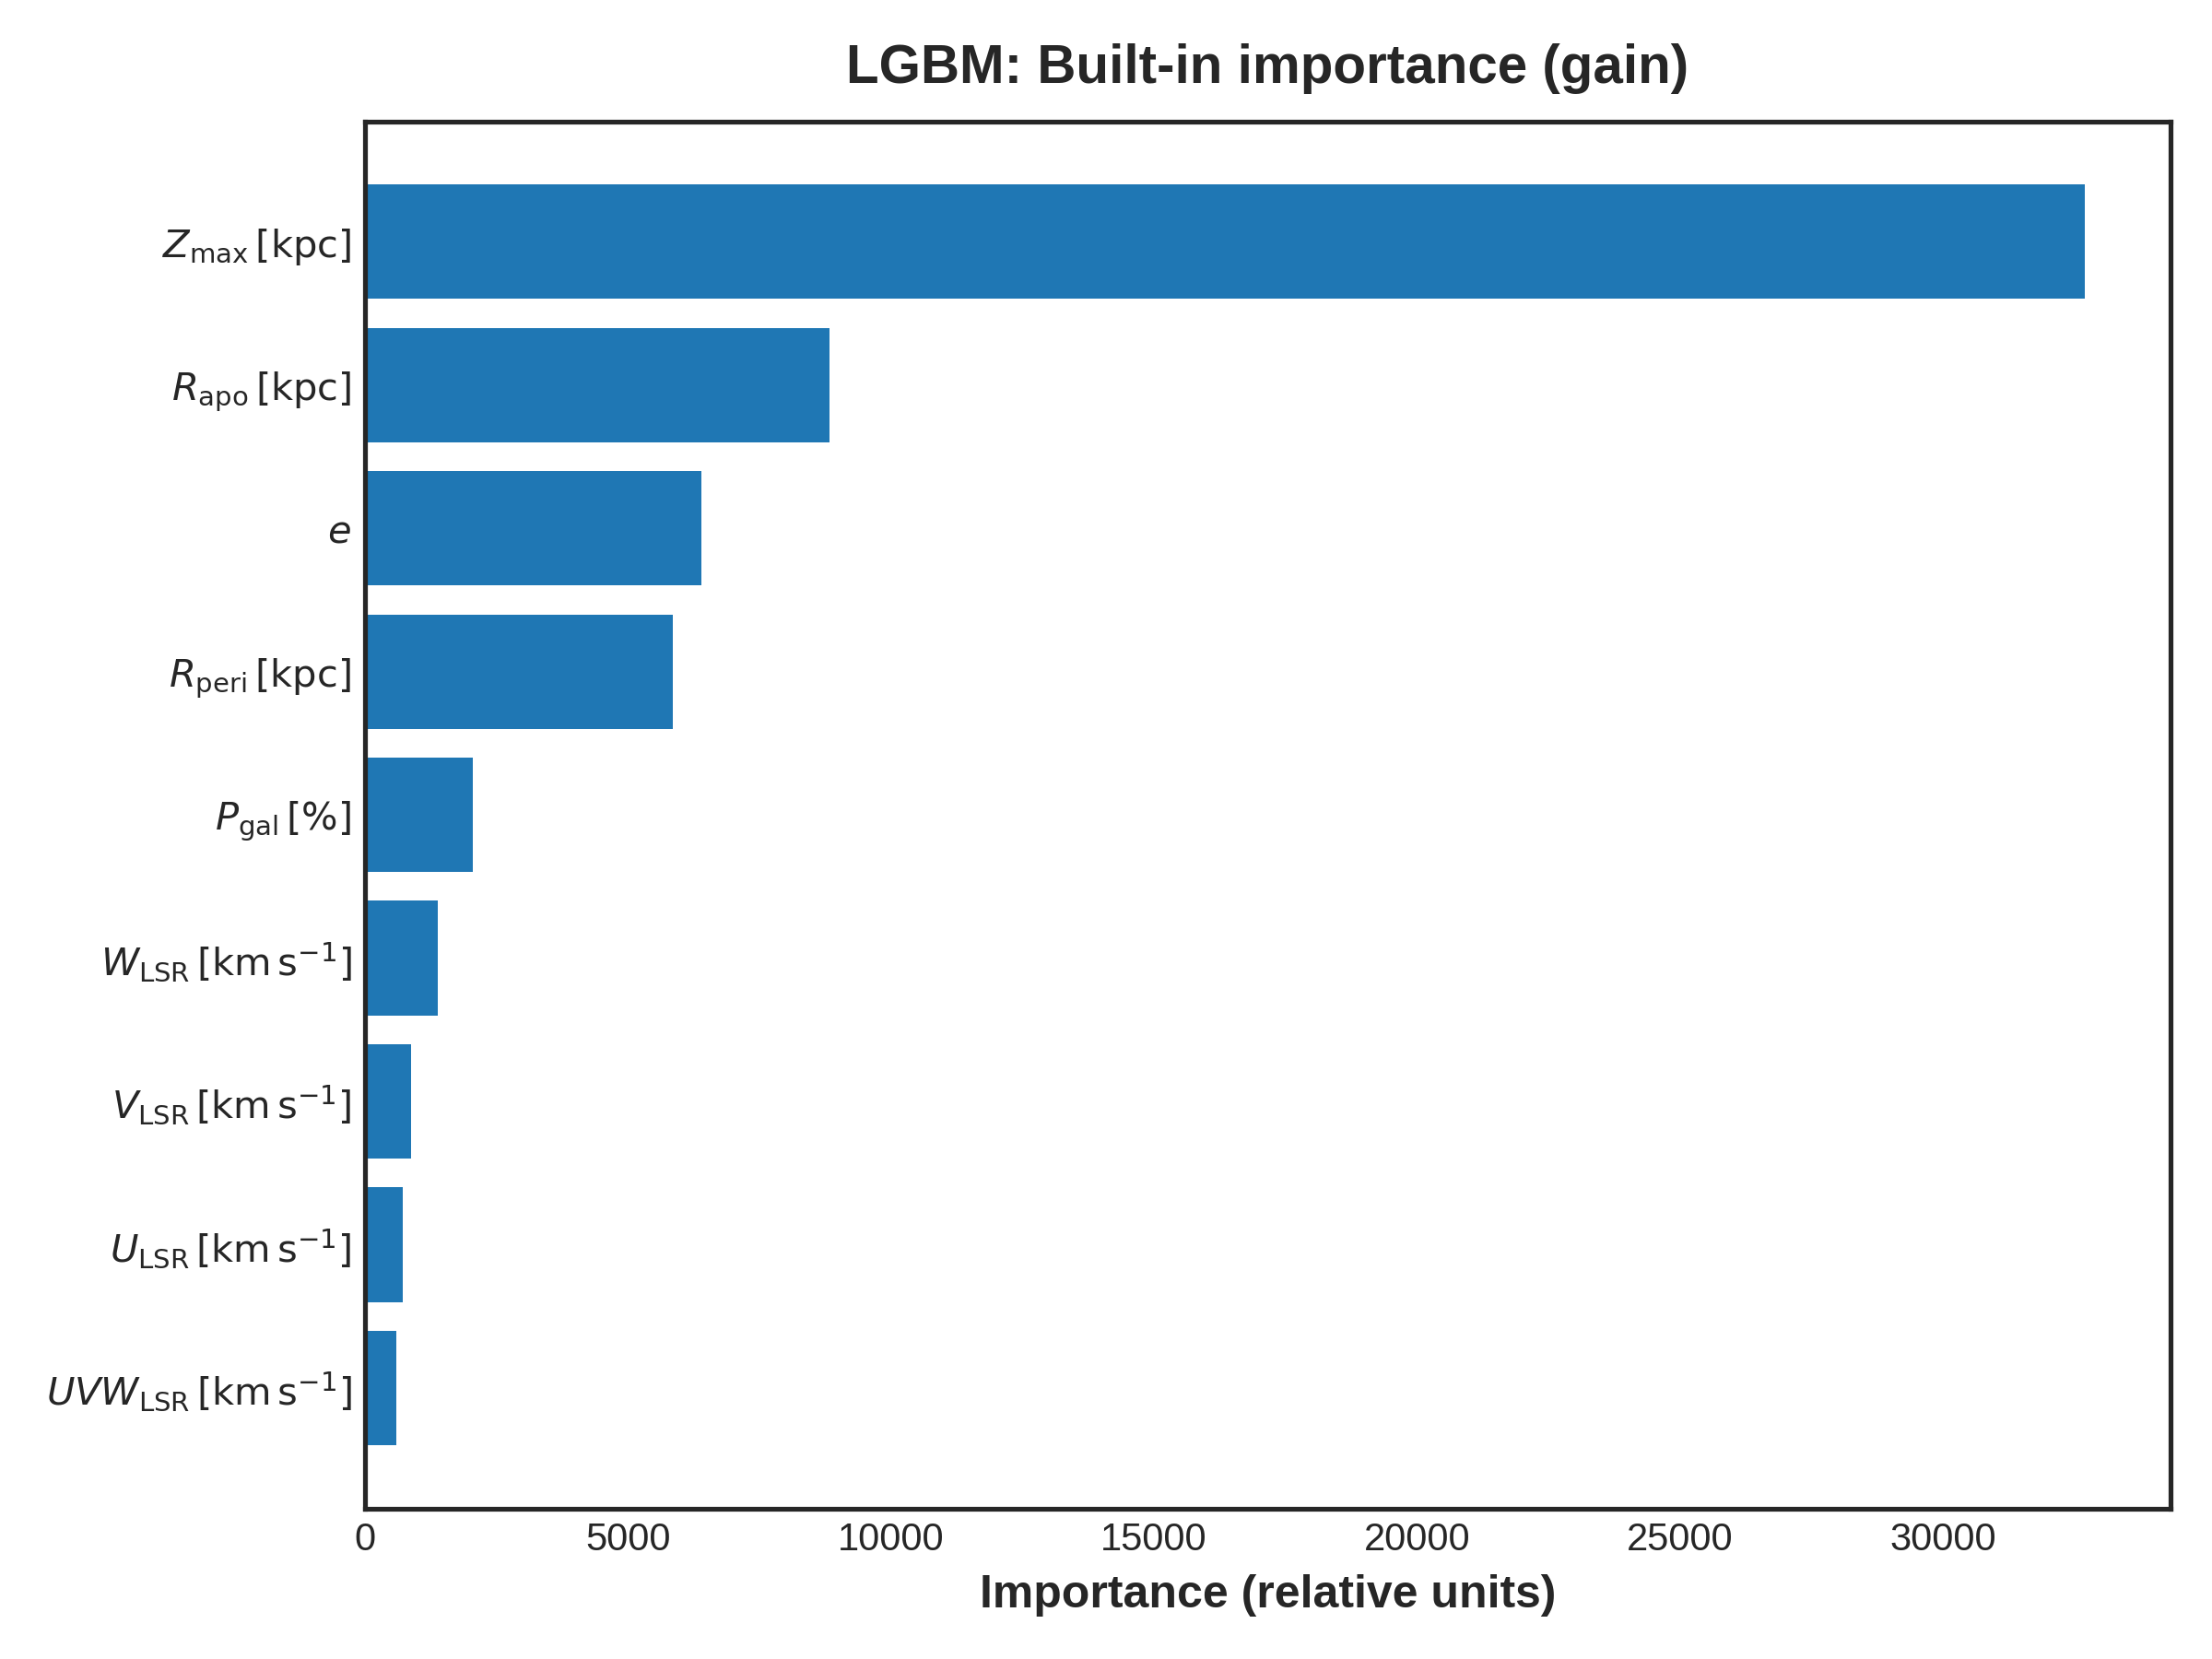
\includegraphics[width=0.24\textwidth]{figures/LGBM_builtin_gain.png}
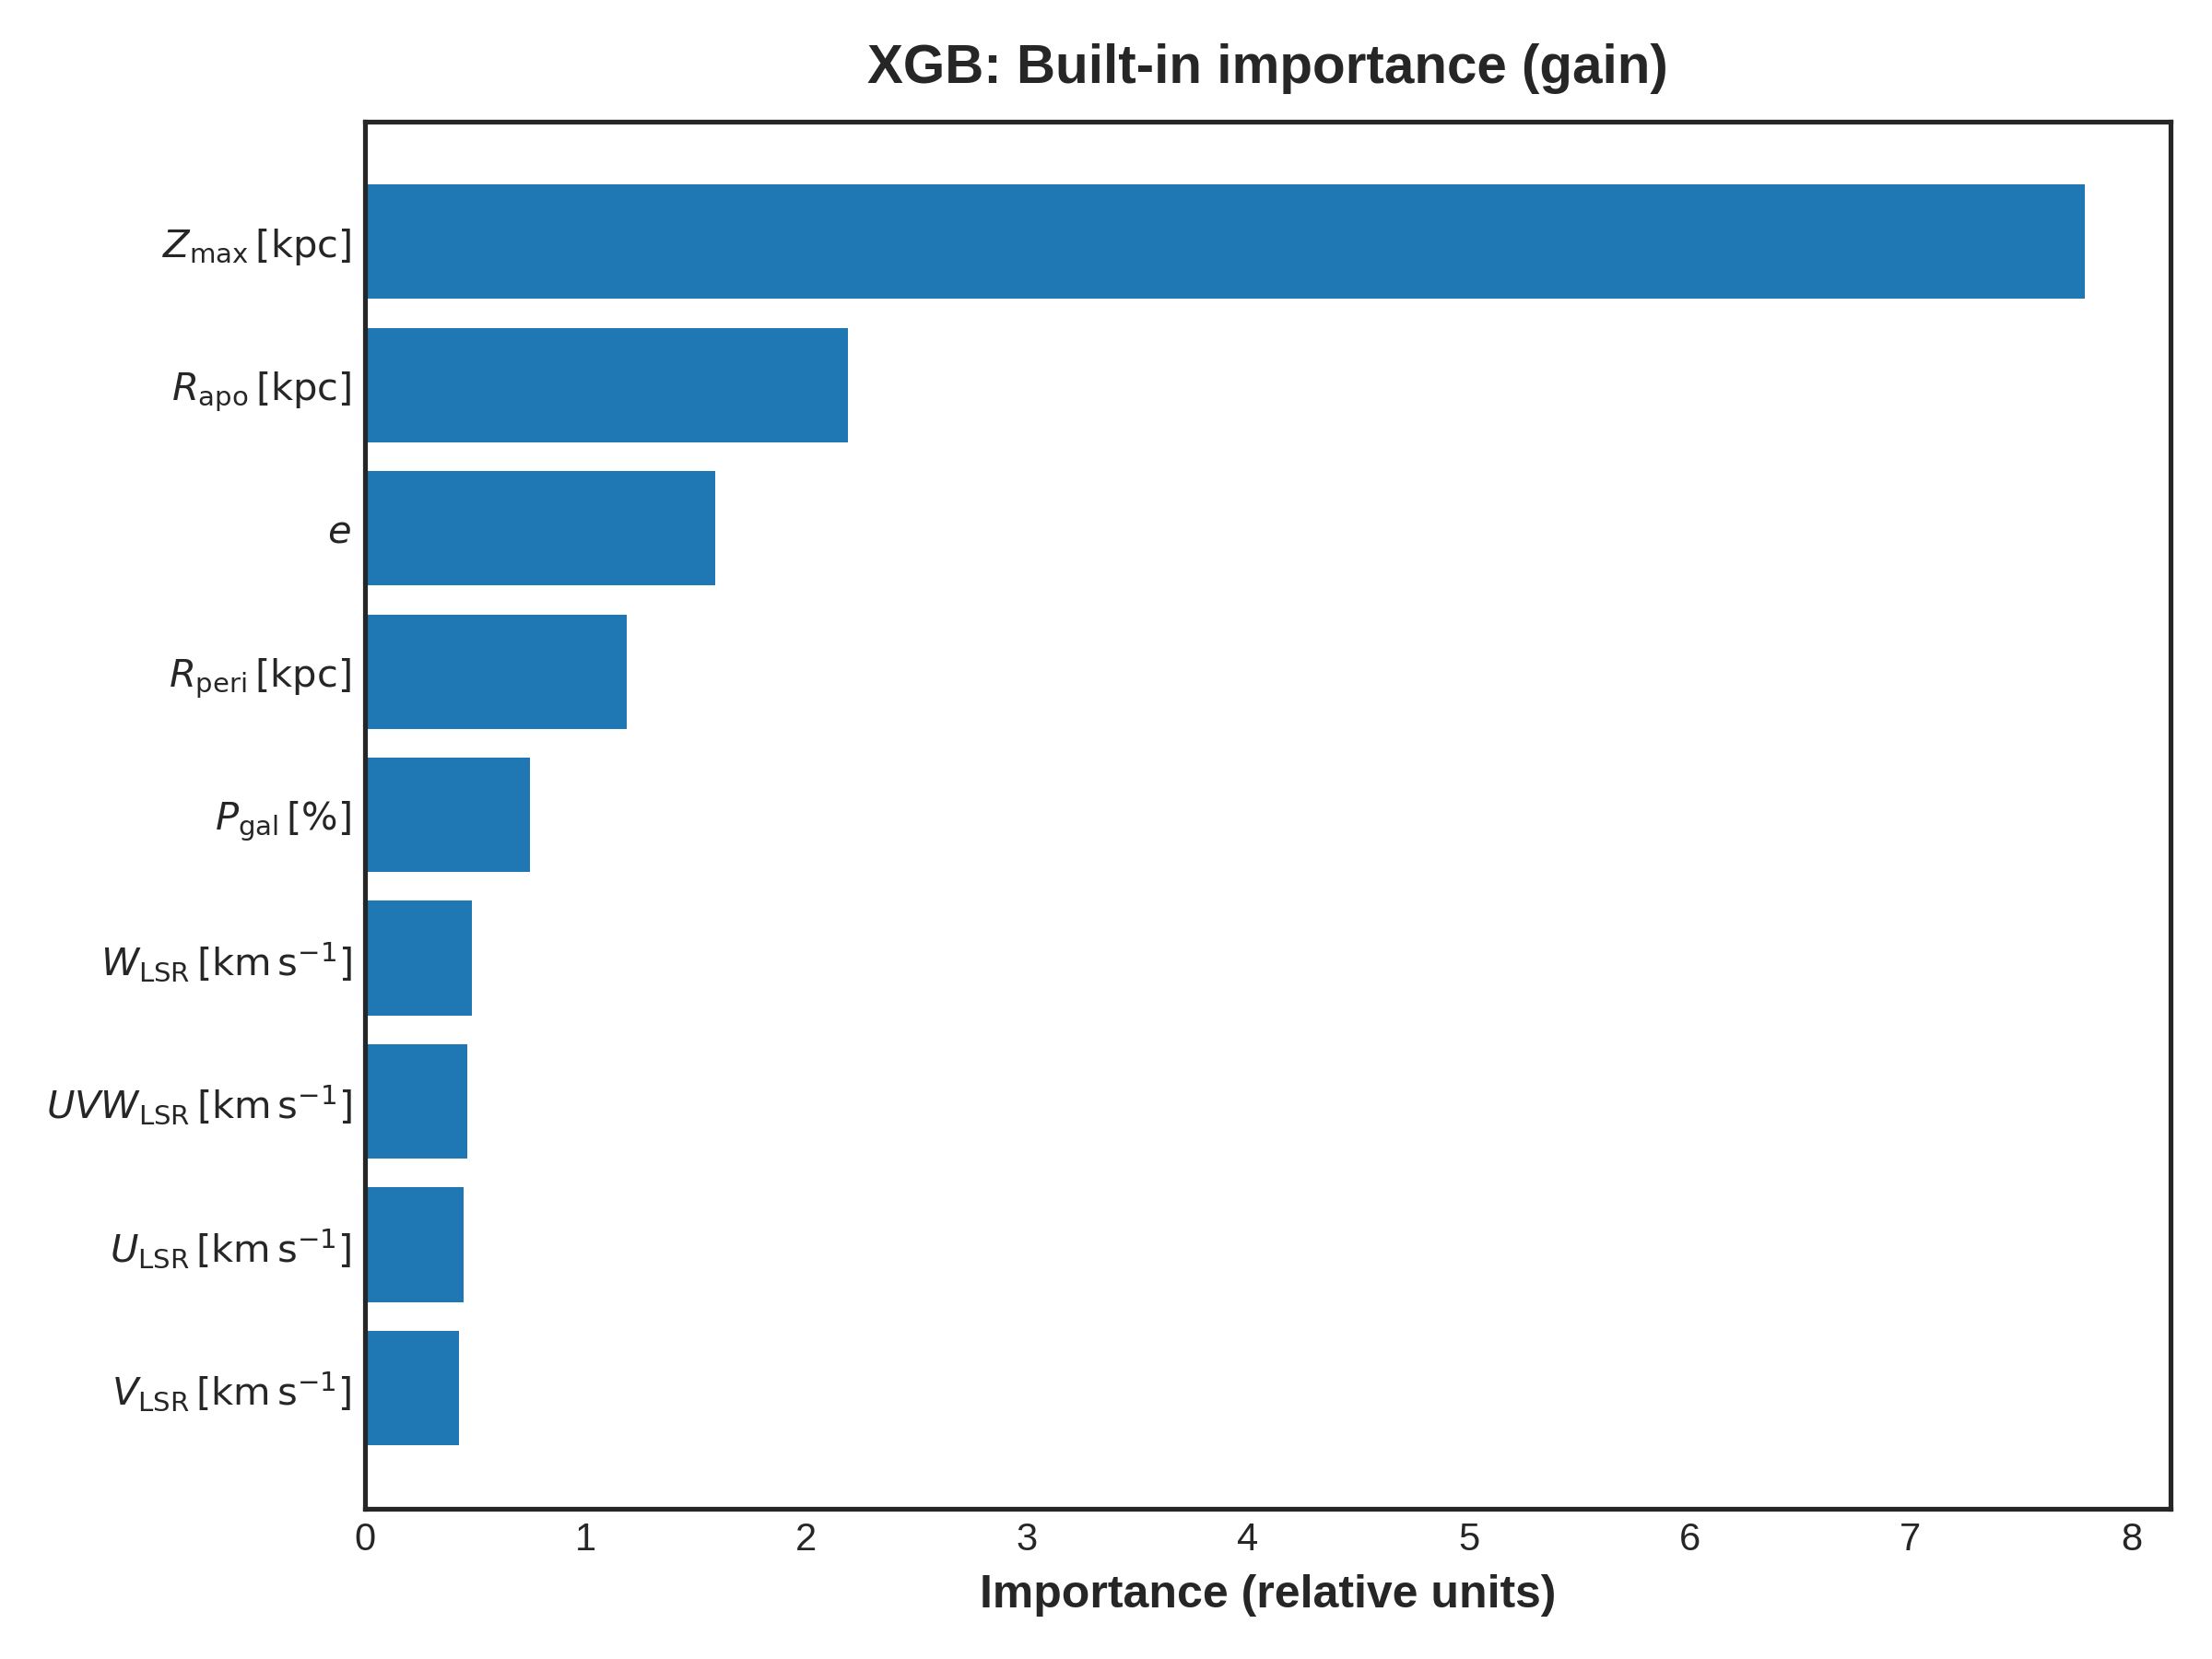
\includegraphics[width=0.24\textwidth]{figures/XGB_builtin_gain.png}
\vspace{0.4cm}
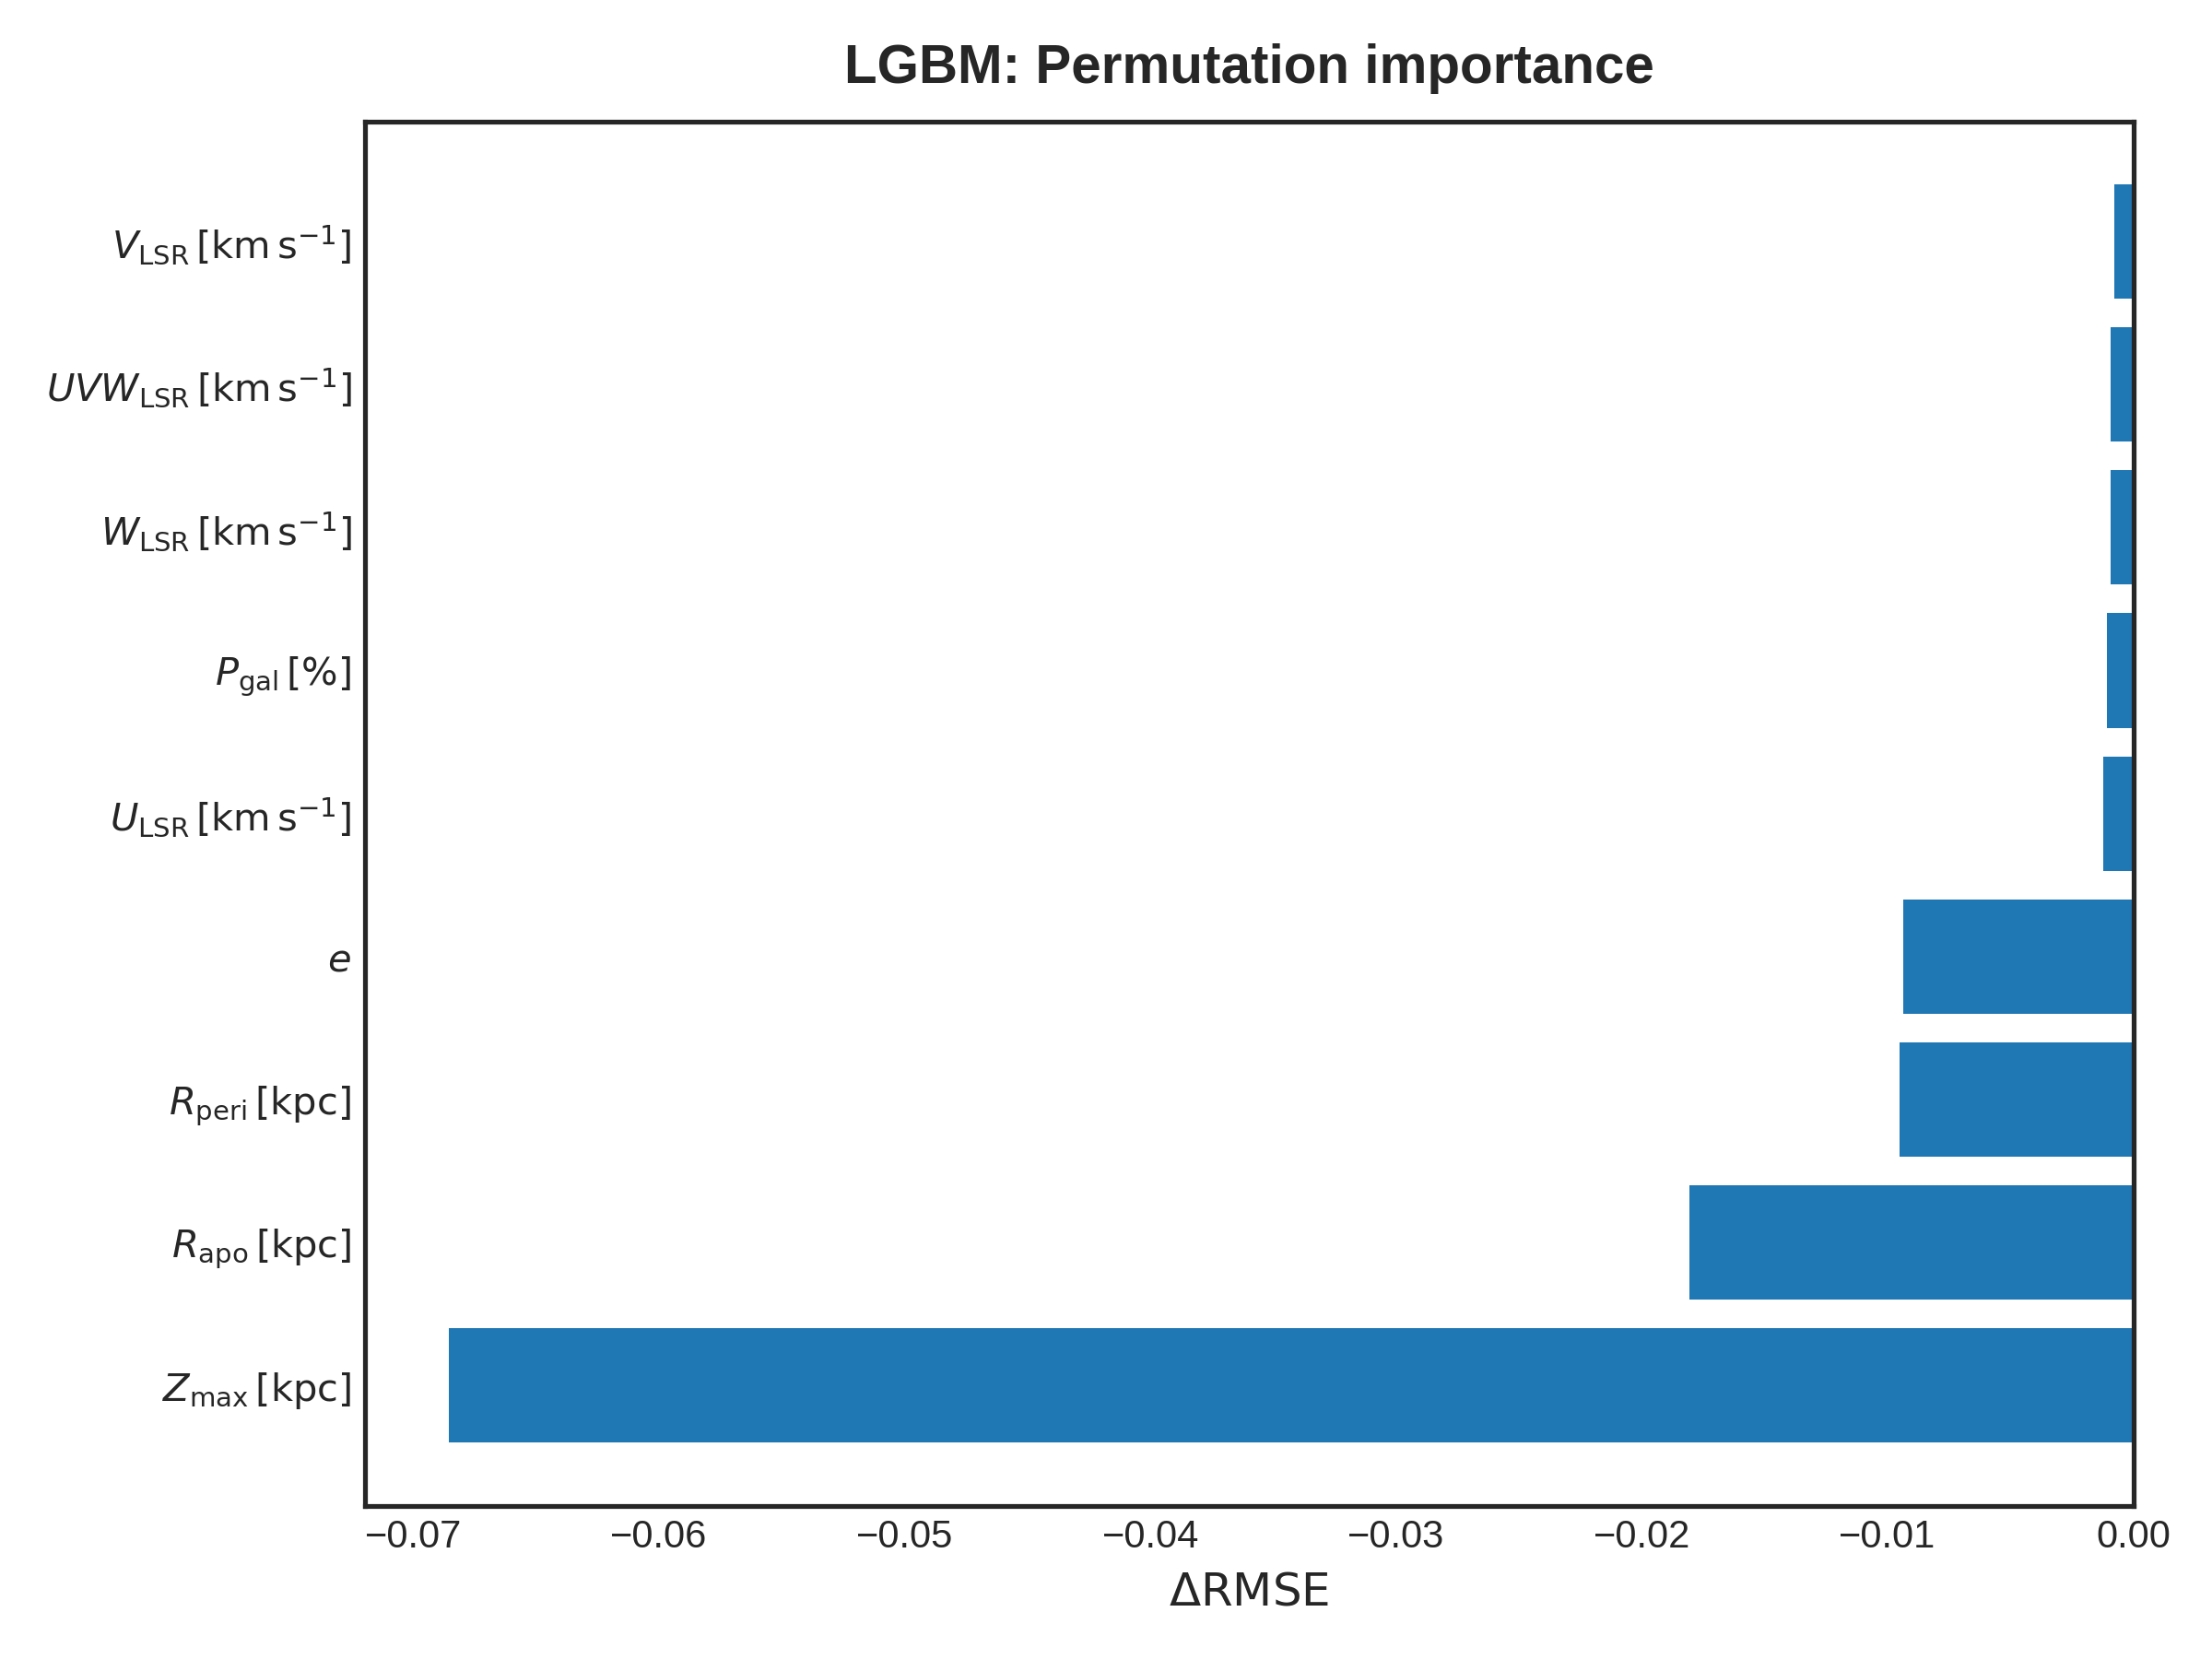
\includegraphics[width=0.24\textwidth]{figures/LGBM_permutation_dRMSE.png}
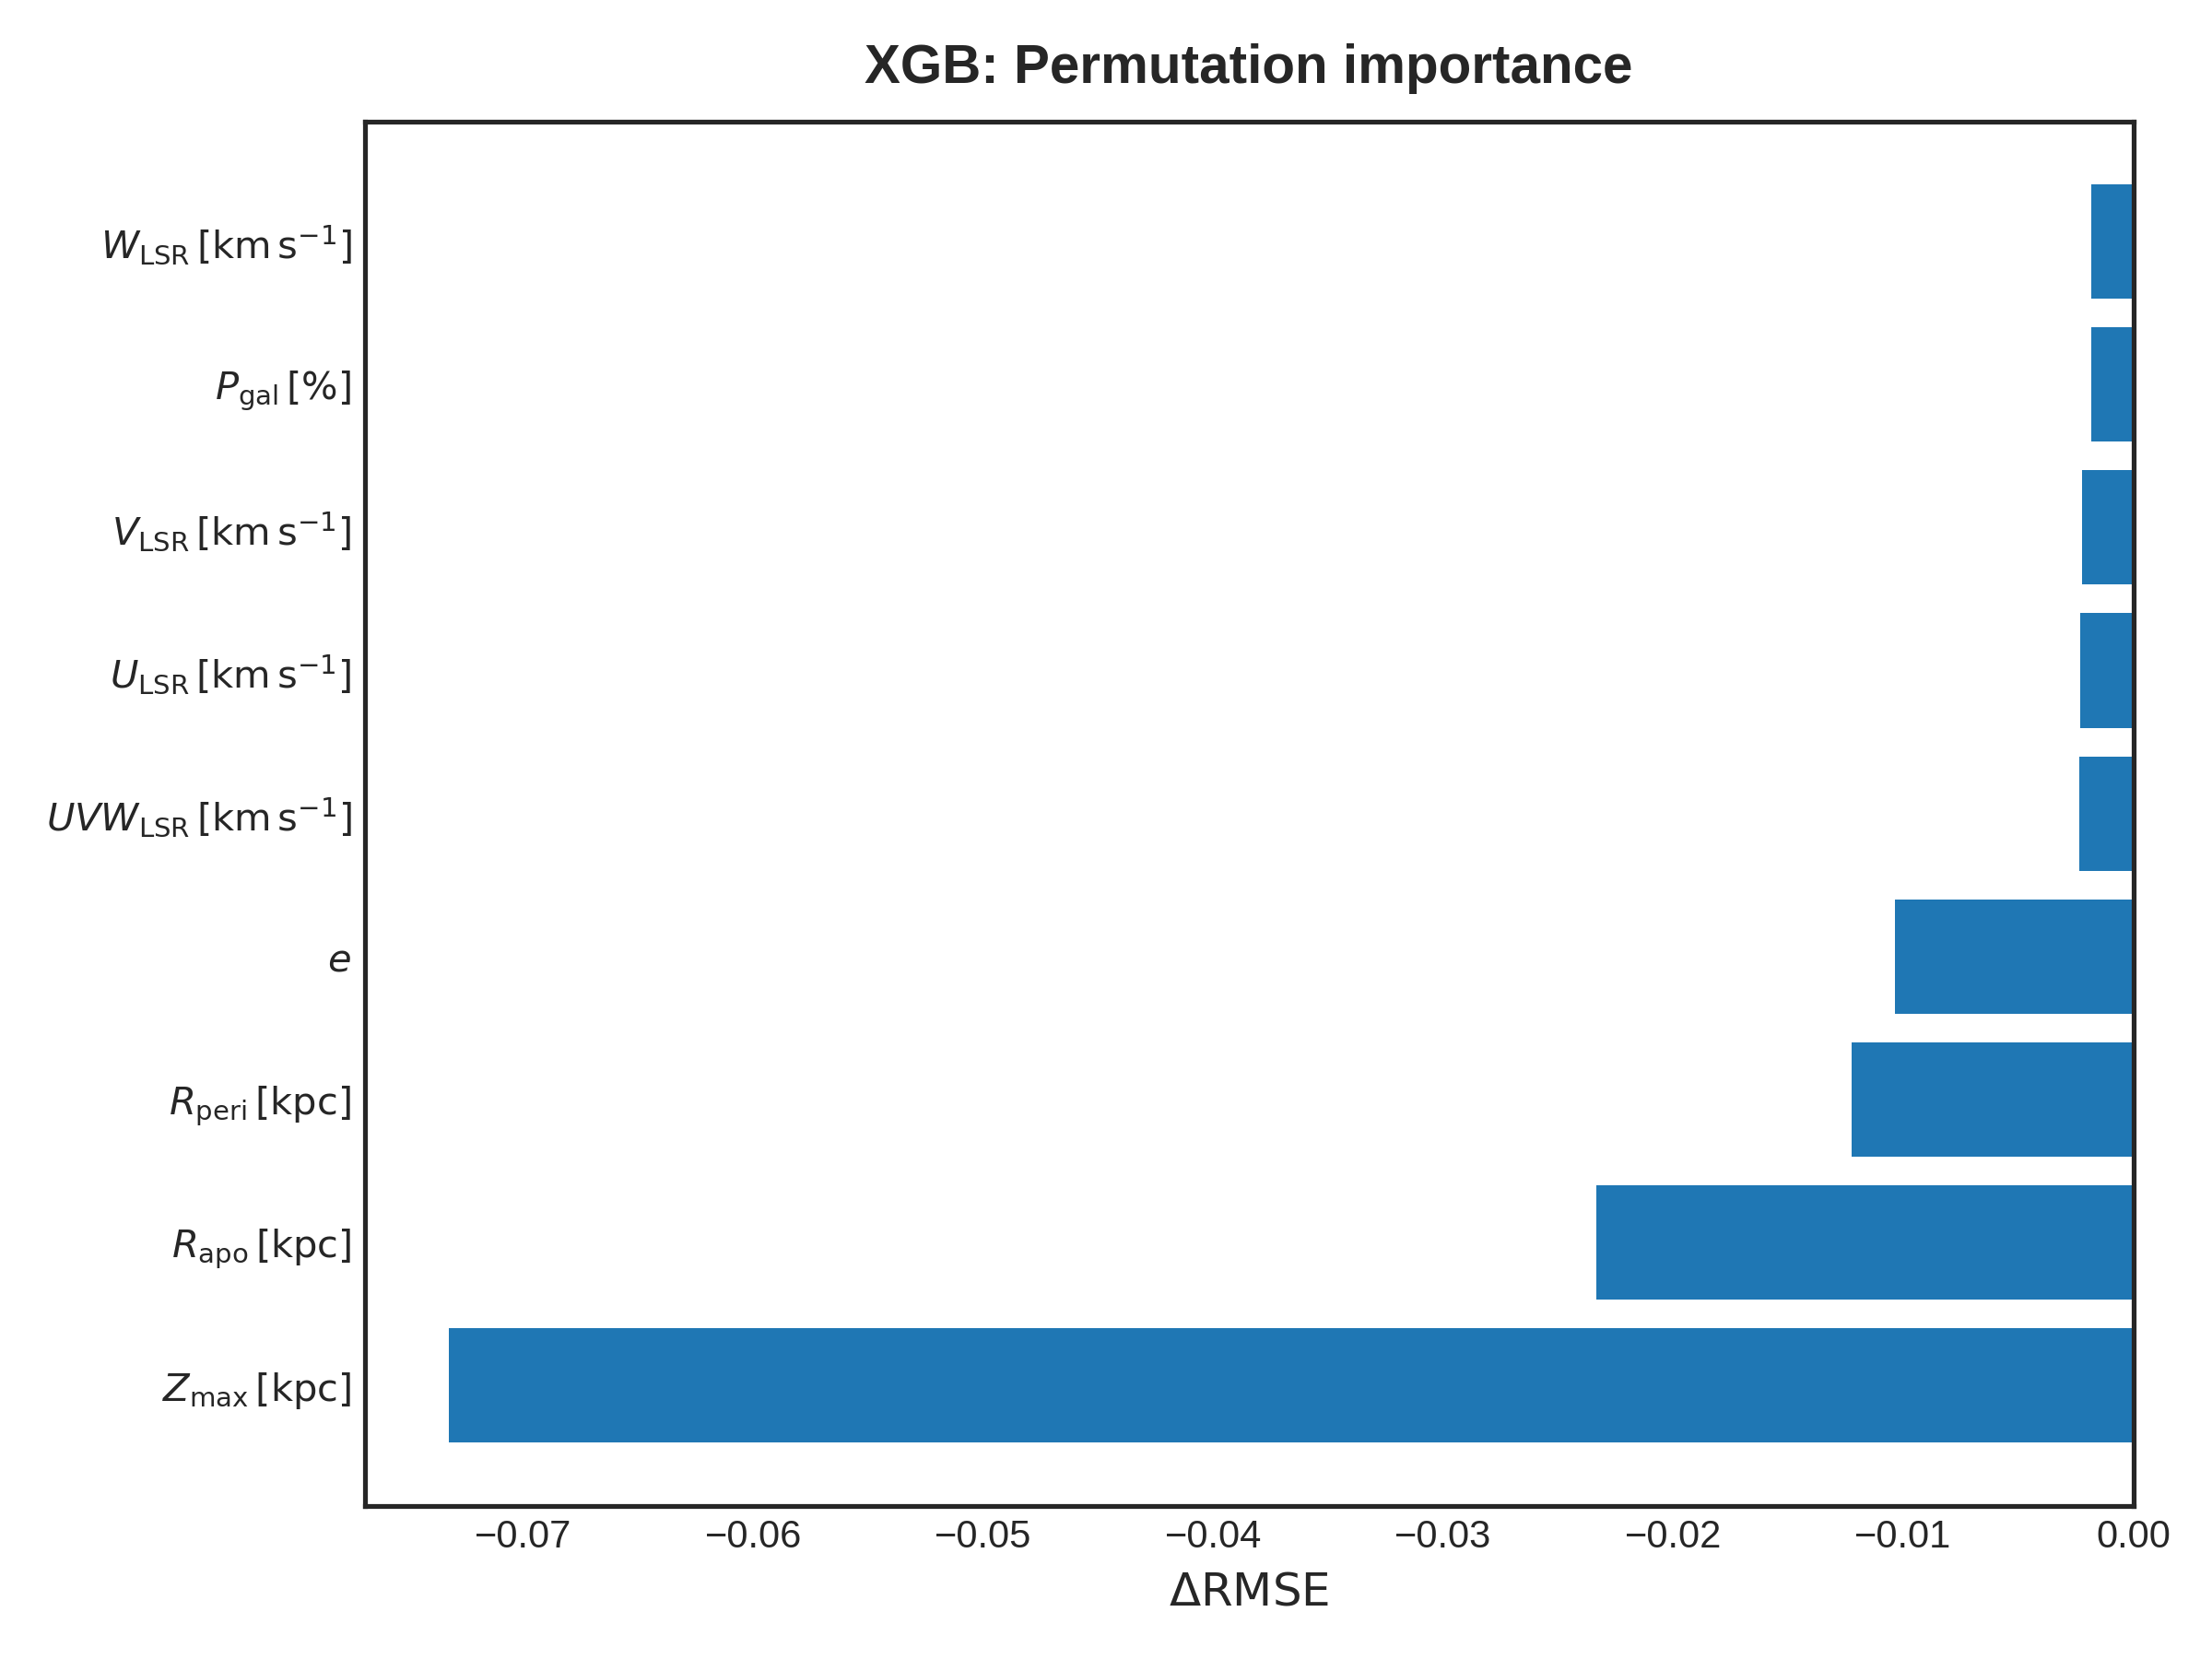
\includegraphics[width=0.24\textwidth]{figures/XGB_permutation_dRMSE.png}
\vspace{0.4cm}
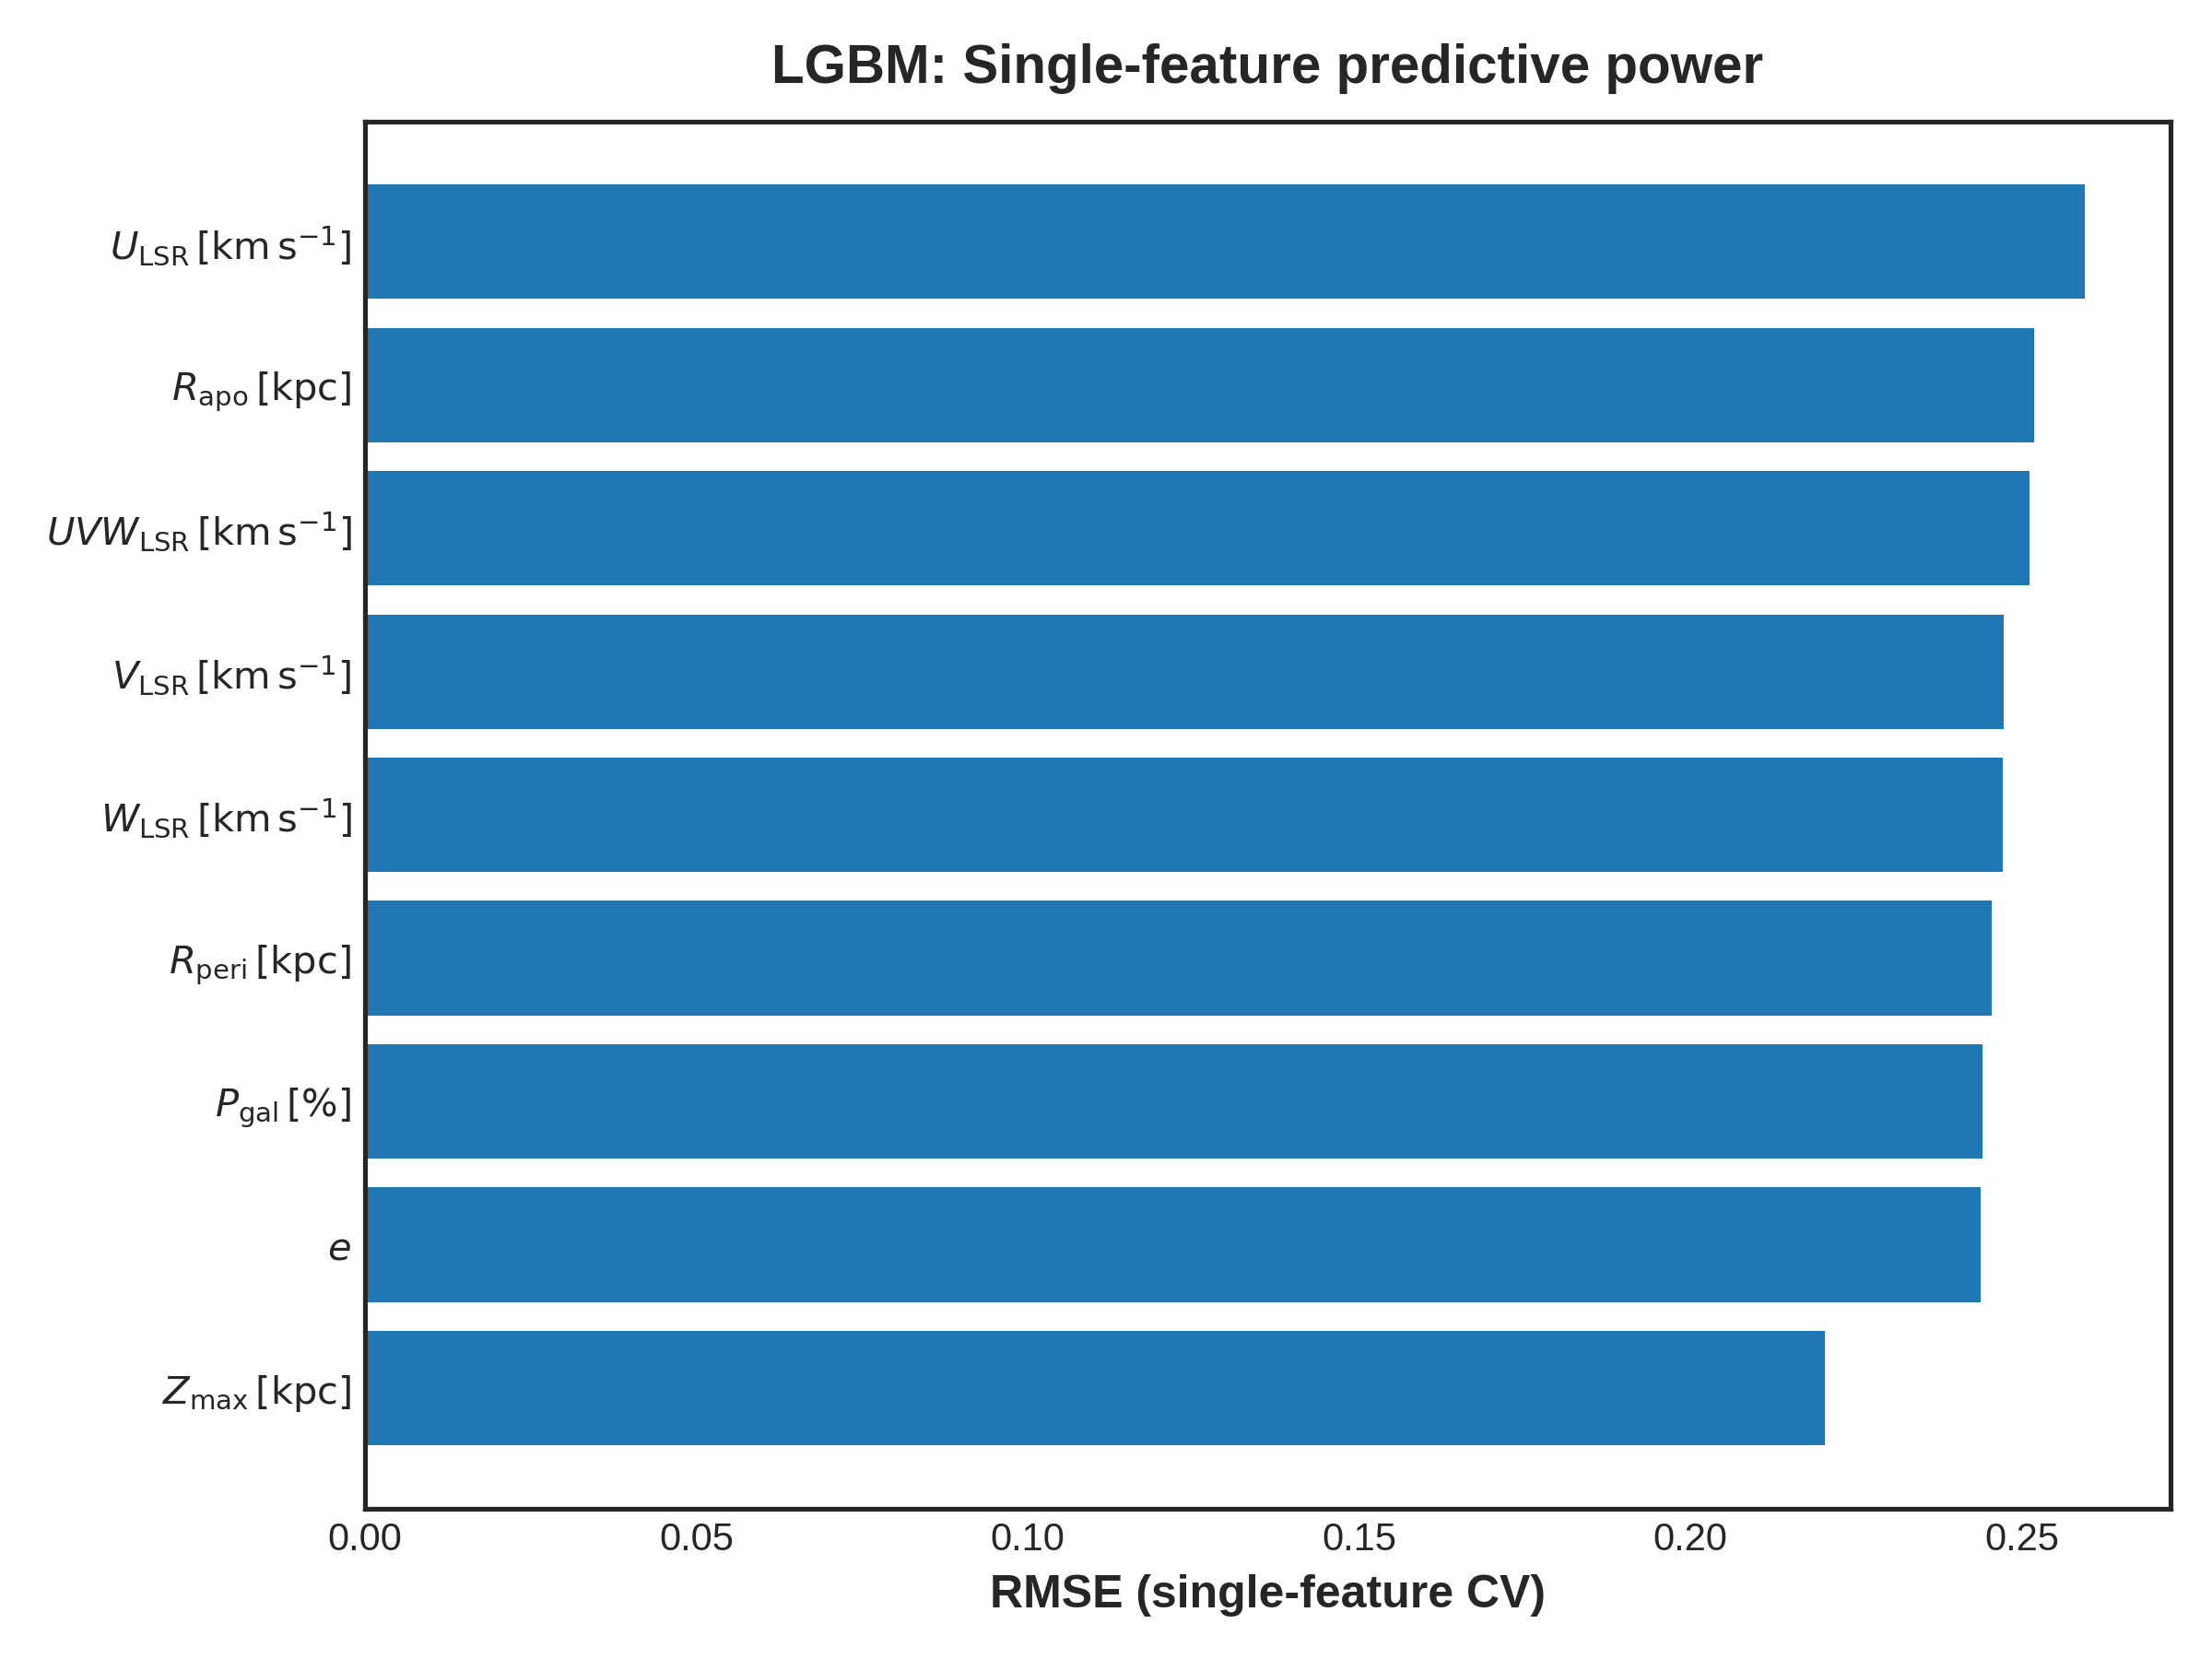
\includegraphics[width=0.24\textwidth]{figures/LGBM_single_feature_rmse.png}
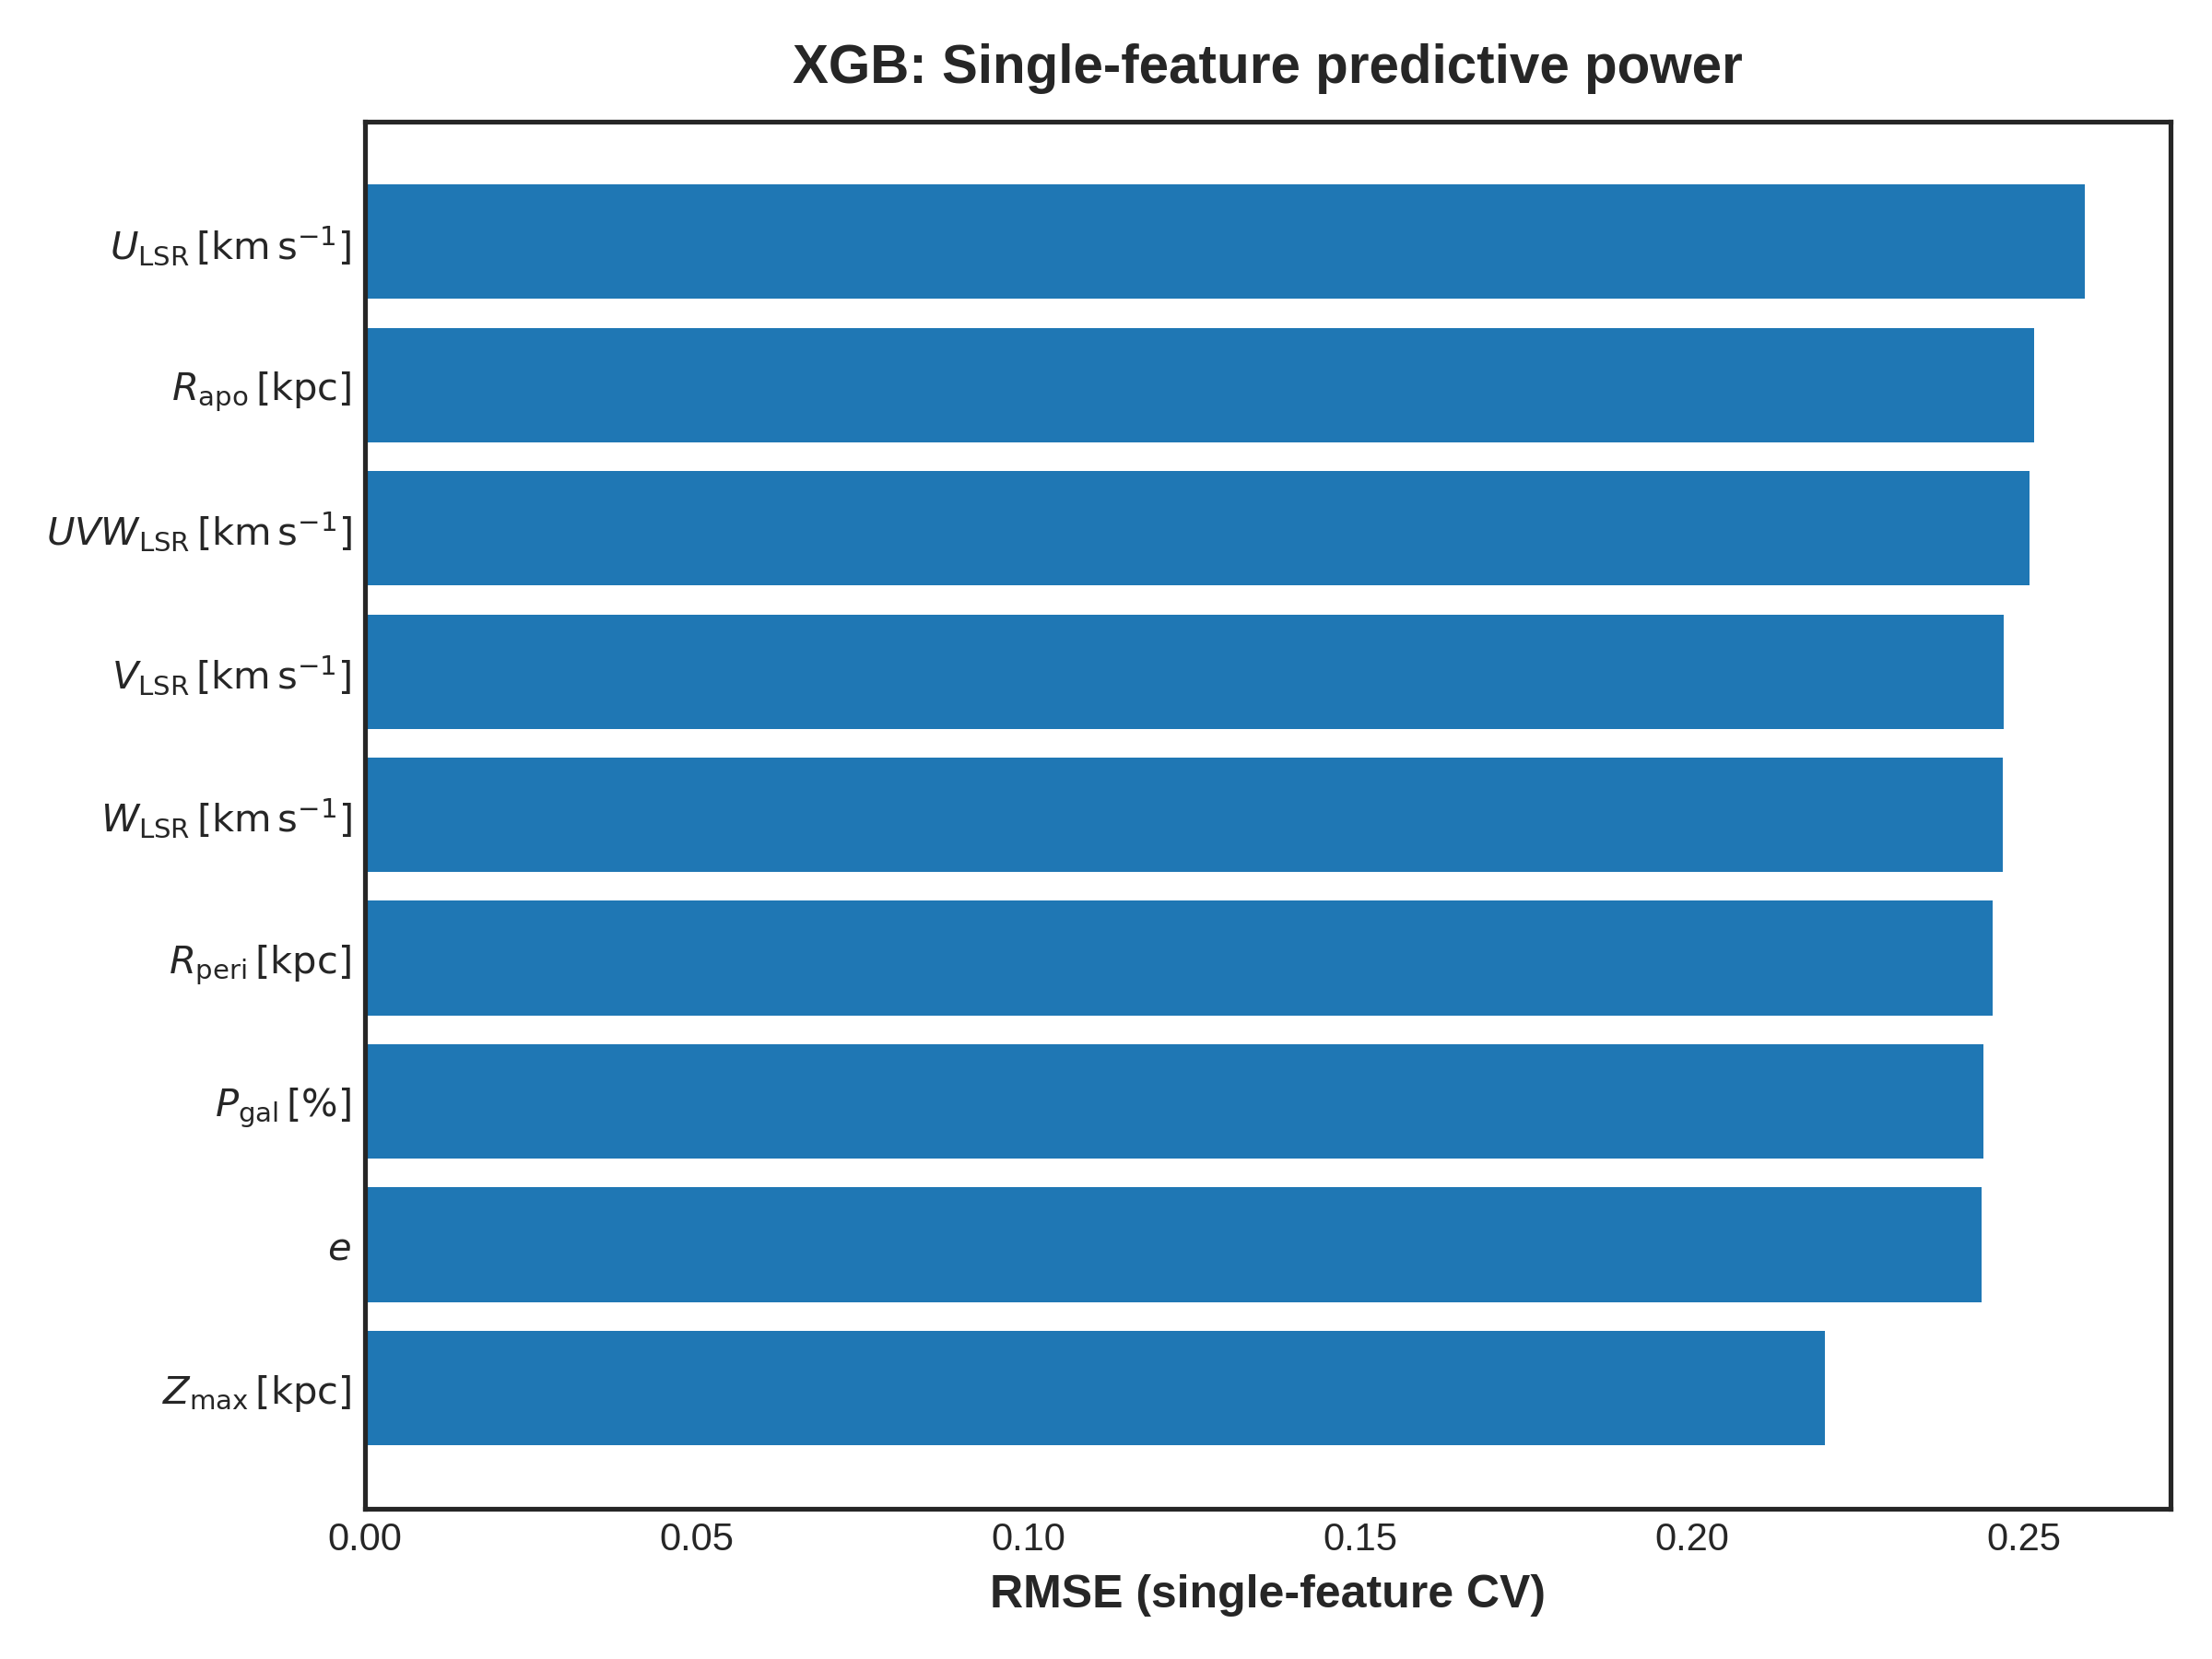
\includegraphics[width=0.24\textwidth]{figures/XGB_single_feature_rmse.png}
\vspace{0.4cm}
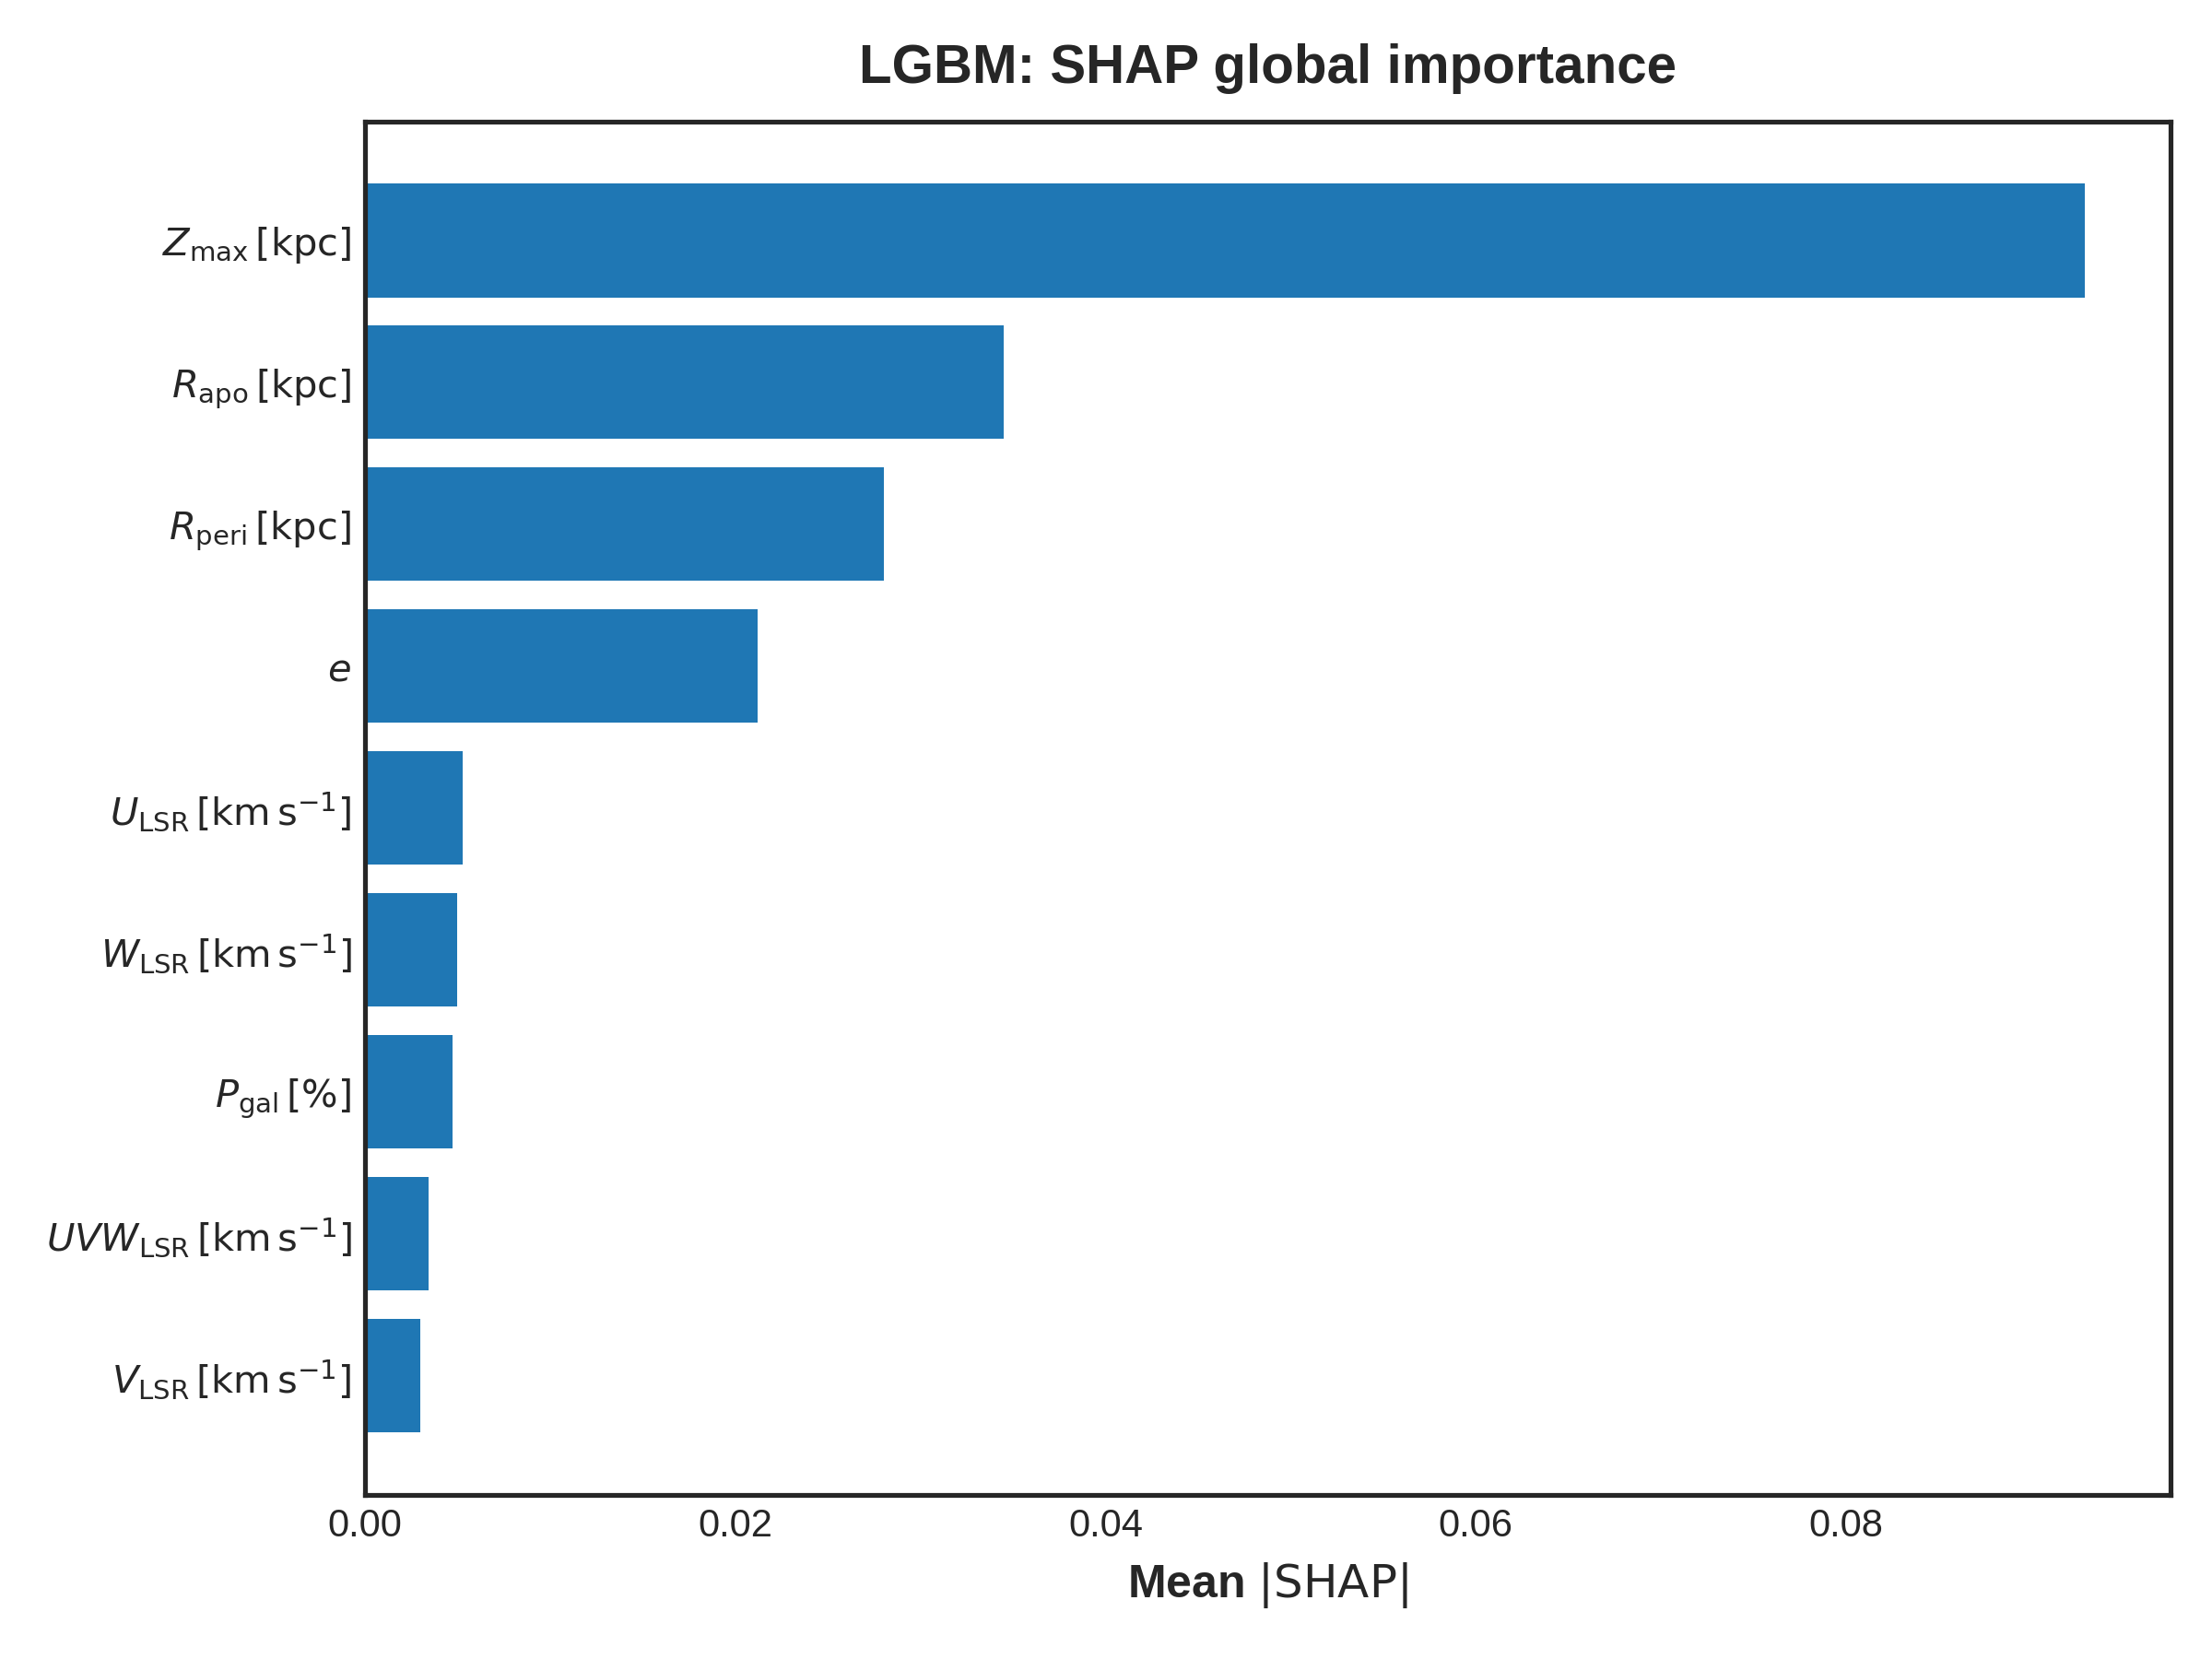
\includegraphics[width=0.24\textwidth]{figures/LGBM_shap_meanabs.png}
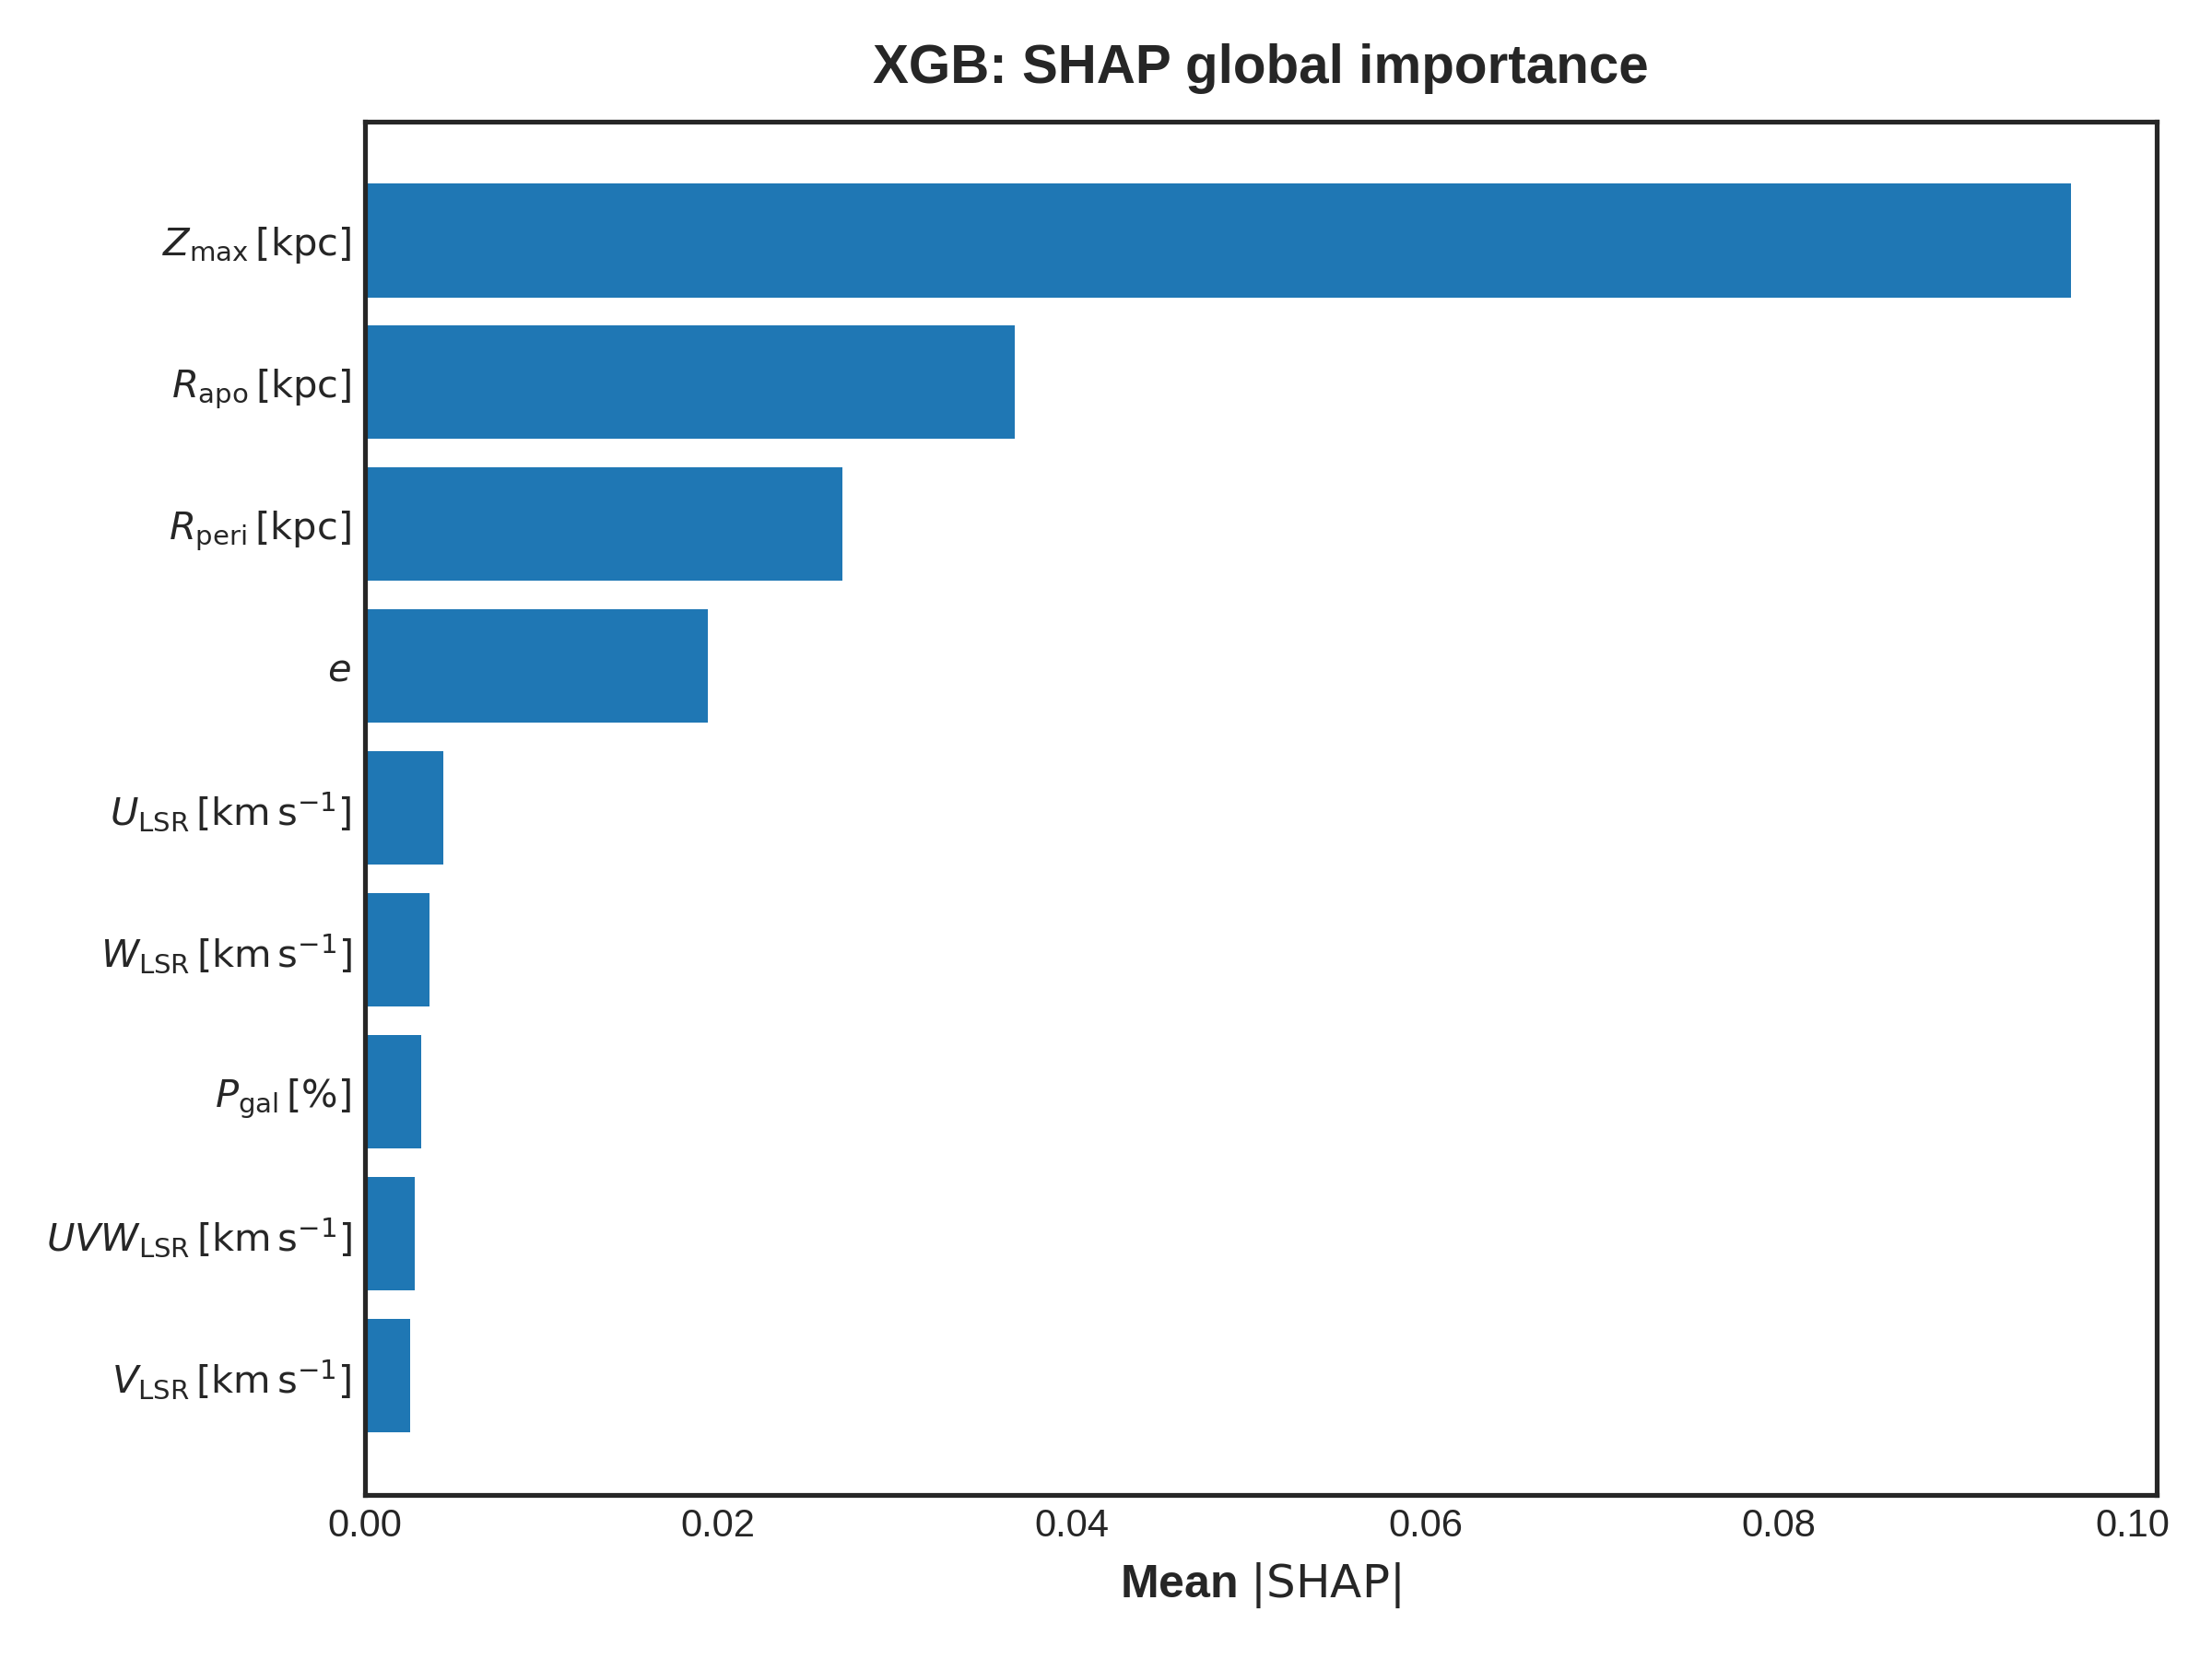
\includegraphics[width=0.24\textwidth]{figures/XGB_shap_meanabs.png}
\caption{Feature-importance diagnostics for the tuned LightGBM and XGBoost models predicting [Fe/H]. Built-in gain feature importance derived from the gradient boosting trees (top). Permutation feature importance, measured as the increase in prediction error ($\Delta$RMSE) after randomly shuffling each feature (second to top).  Predictive performance (RMSE from cross-validation) obtained when training the model using only a single feature at a time (second to bottom). Global SHAP importance, showing the mean absolute SHAP value for each feature (bottom).}
\label{fig:feature_importance_feh}
\end{figure}




\section{Predicting individual abundances from metallicity and kinematics}
\label{appendix:abundances}

This appendix provides additional material related to the prediction of individual elemental abundances using stellar metallicity together with kinematic and orbital parameters.


\subsection{Correlation and mutual information analysis}
\label{appendix:correlations_mi_abund}

This appendix presents the full set of Spearman rank correlation and mutual information diagrams between the elemental abundances and the input features used in this work. The figures are shown separately for the APOGEE and HARPS samples.

\begin{figure}[ht]
\centering
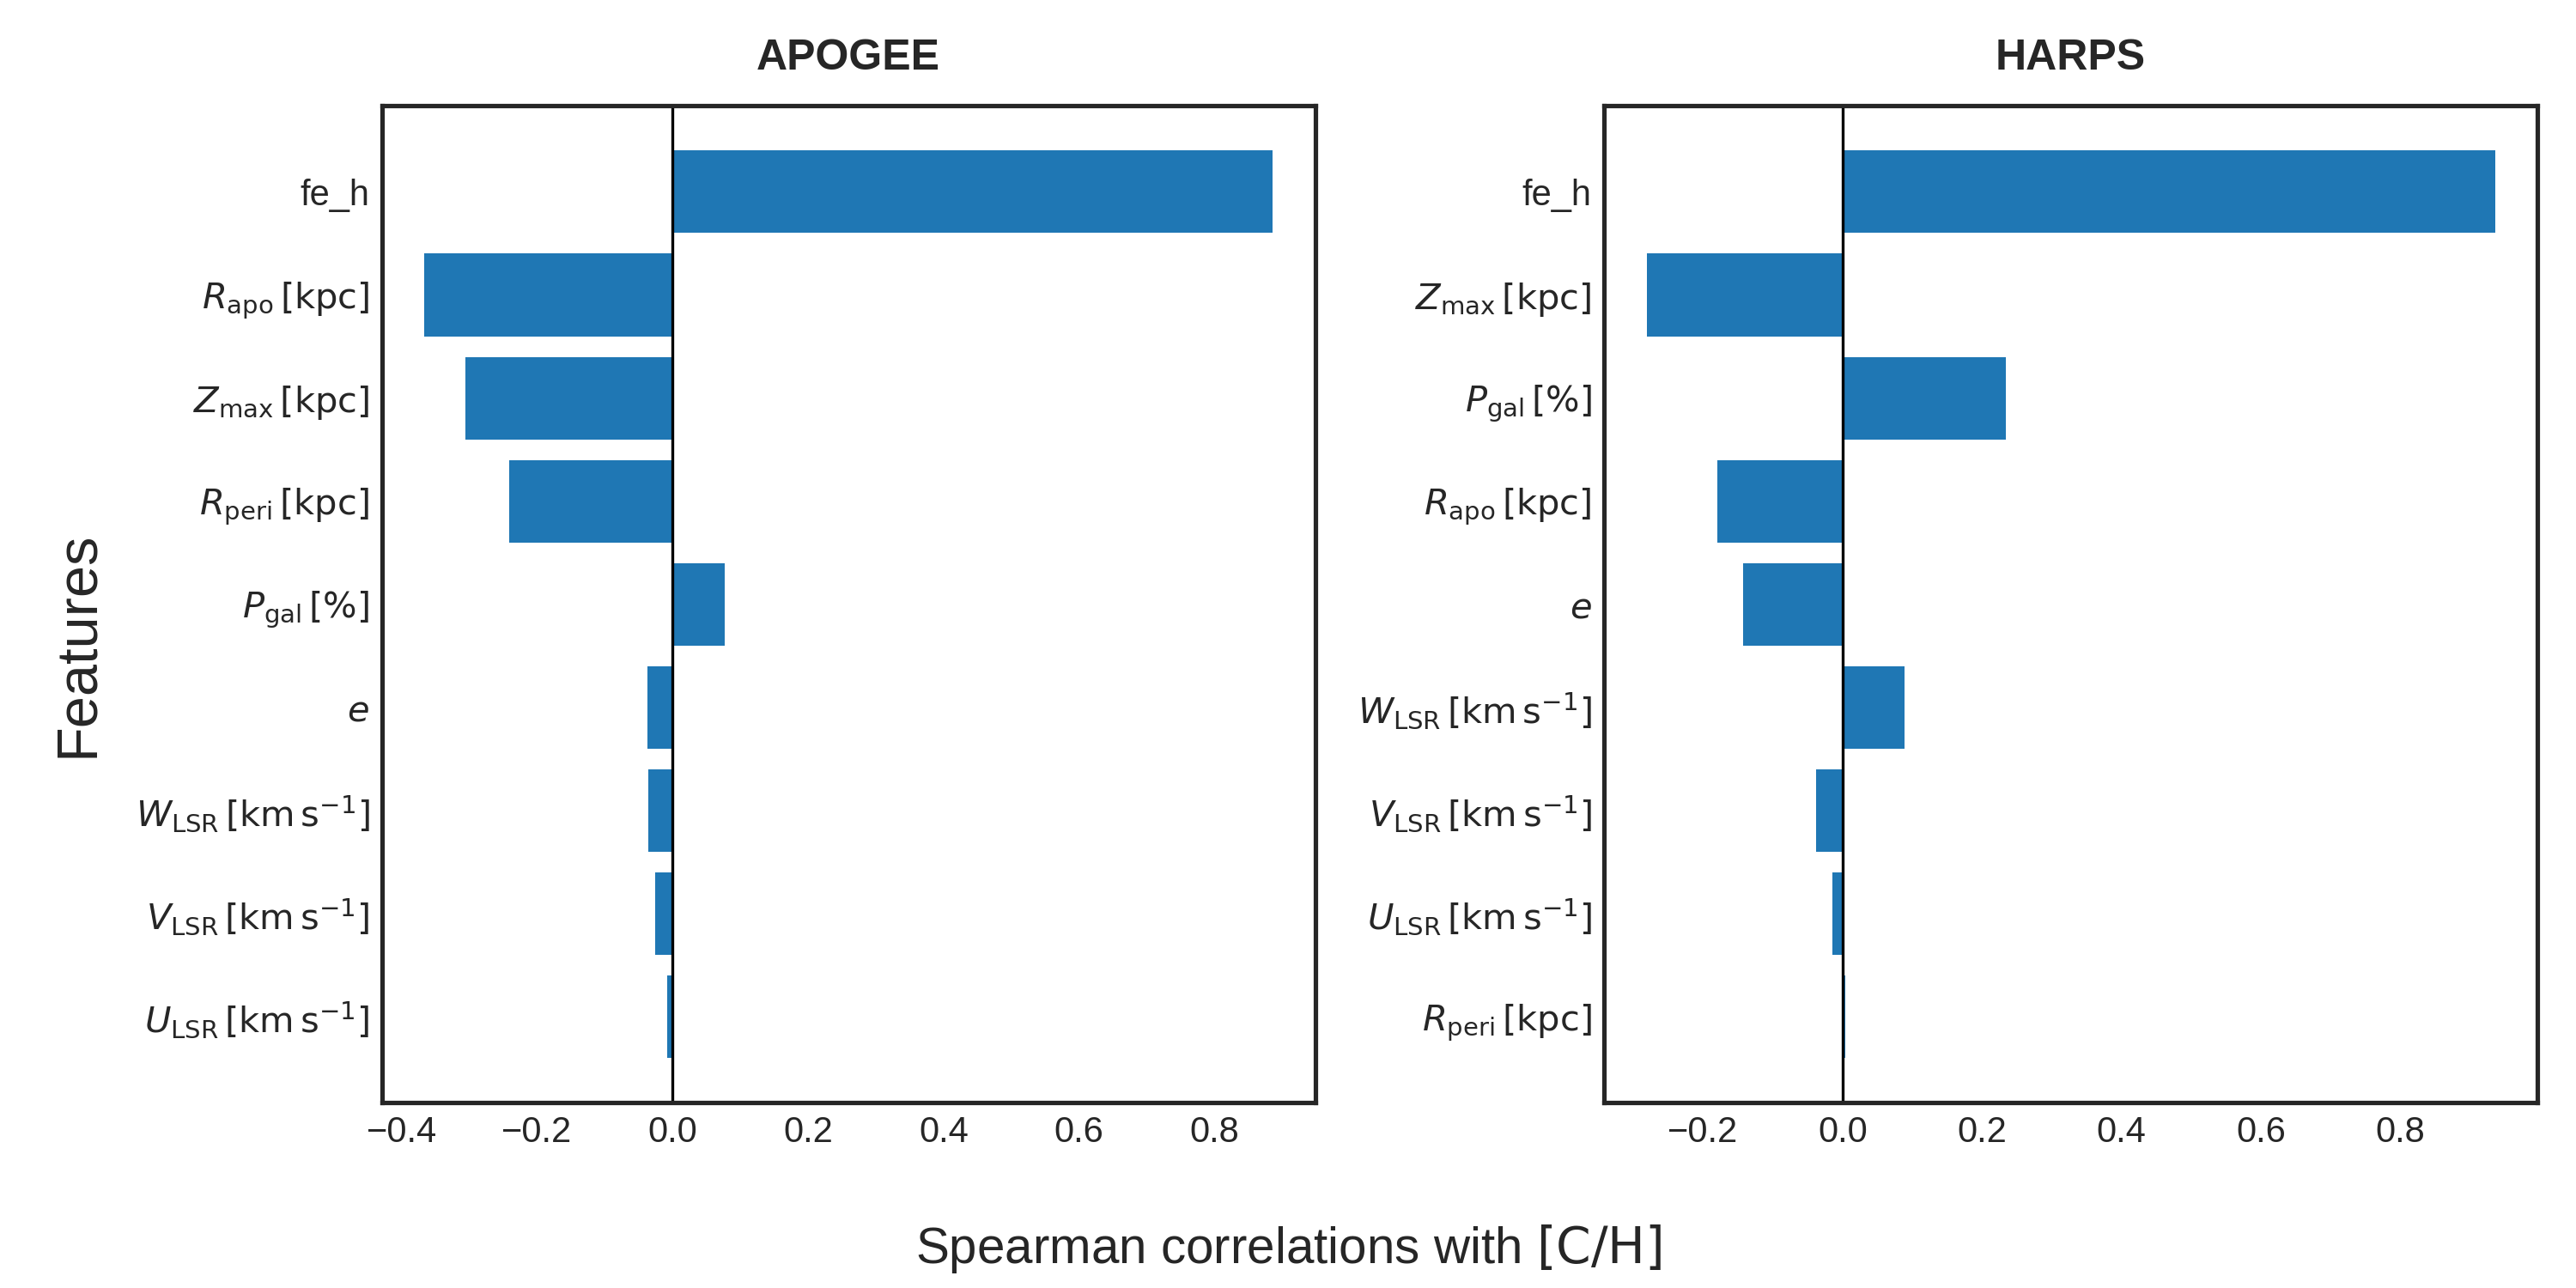
\includegraphics[width=0.48\textwidth]{figures/correlations_c_h.png}
\vspace{0.4cm}
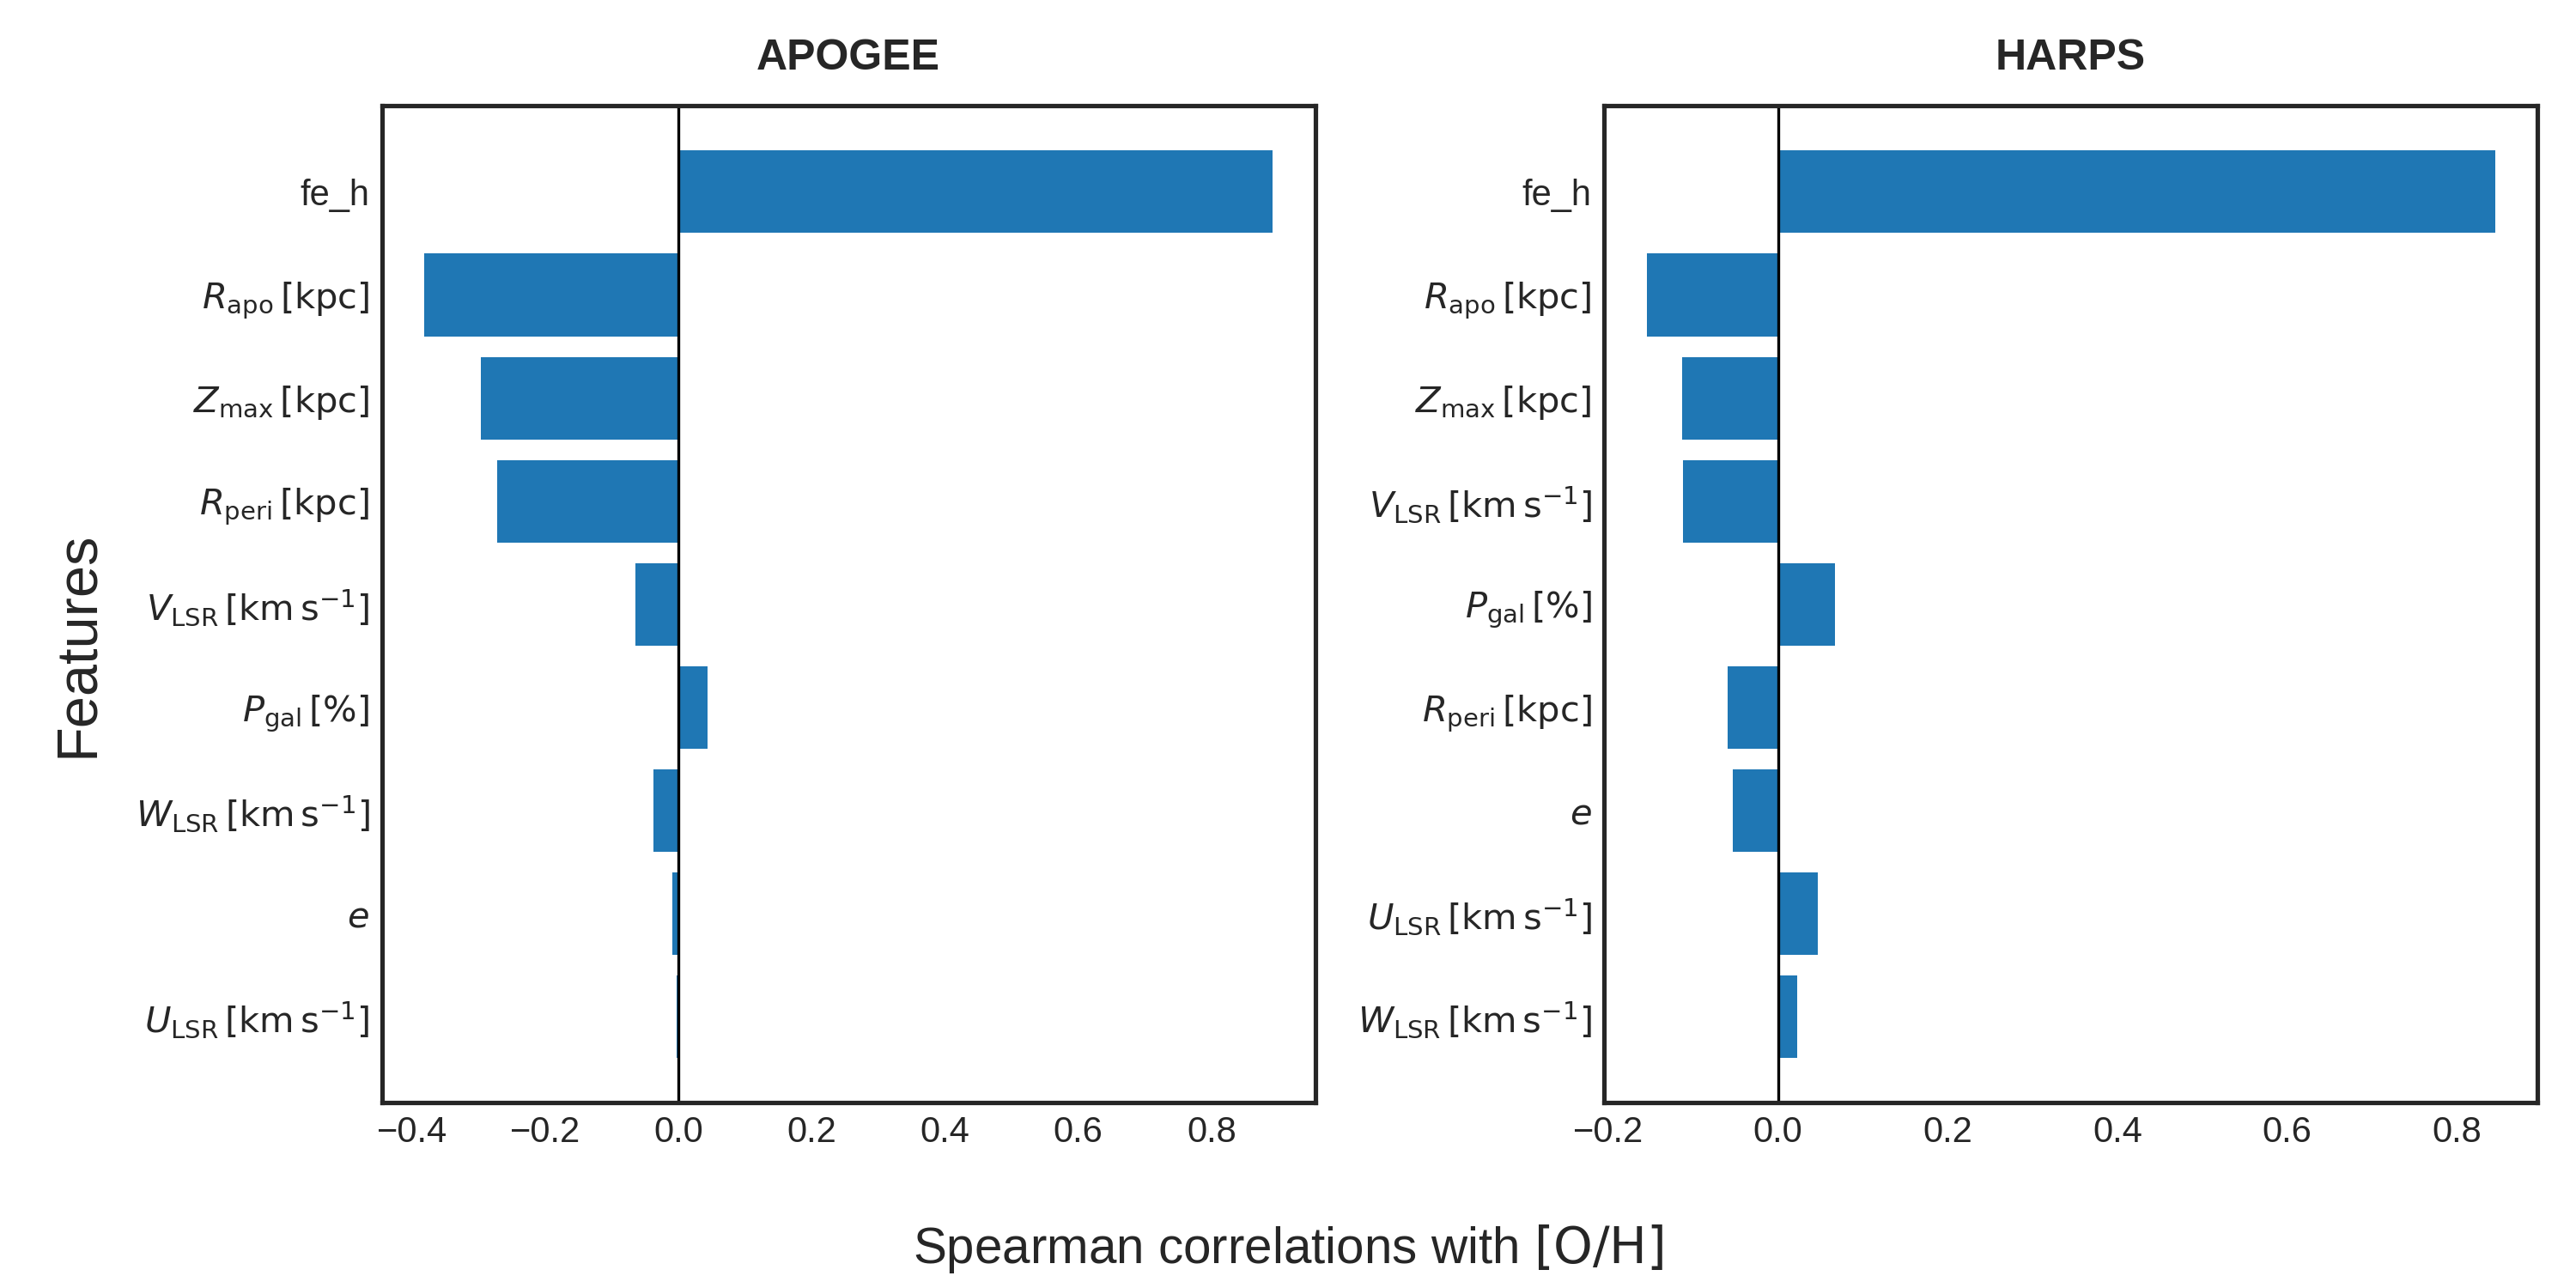
\includegraphics[width=0.48\textwidth]{figures/correlations_o_h.png}
\vspace{0.4cm}
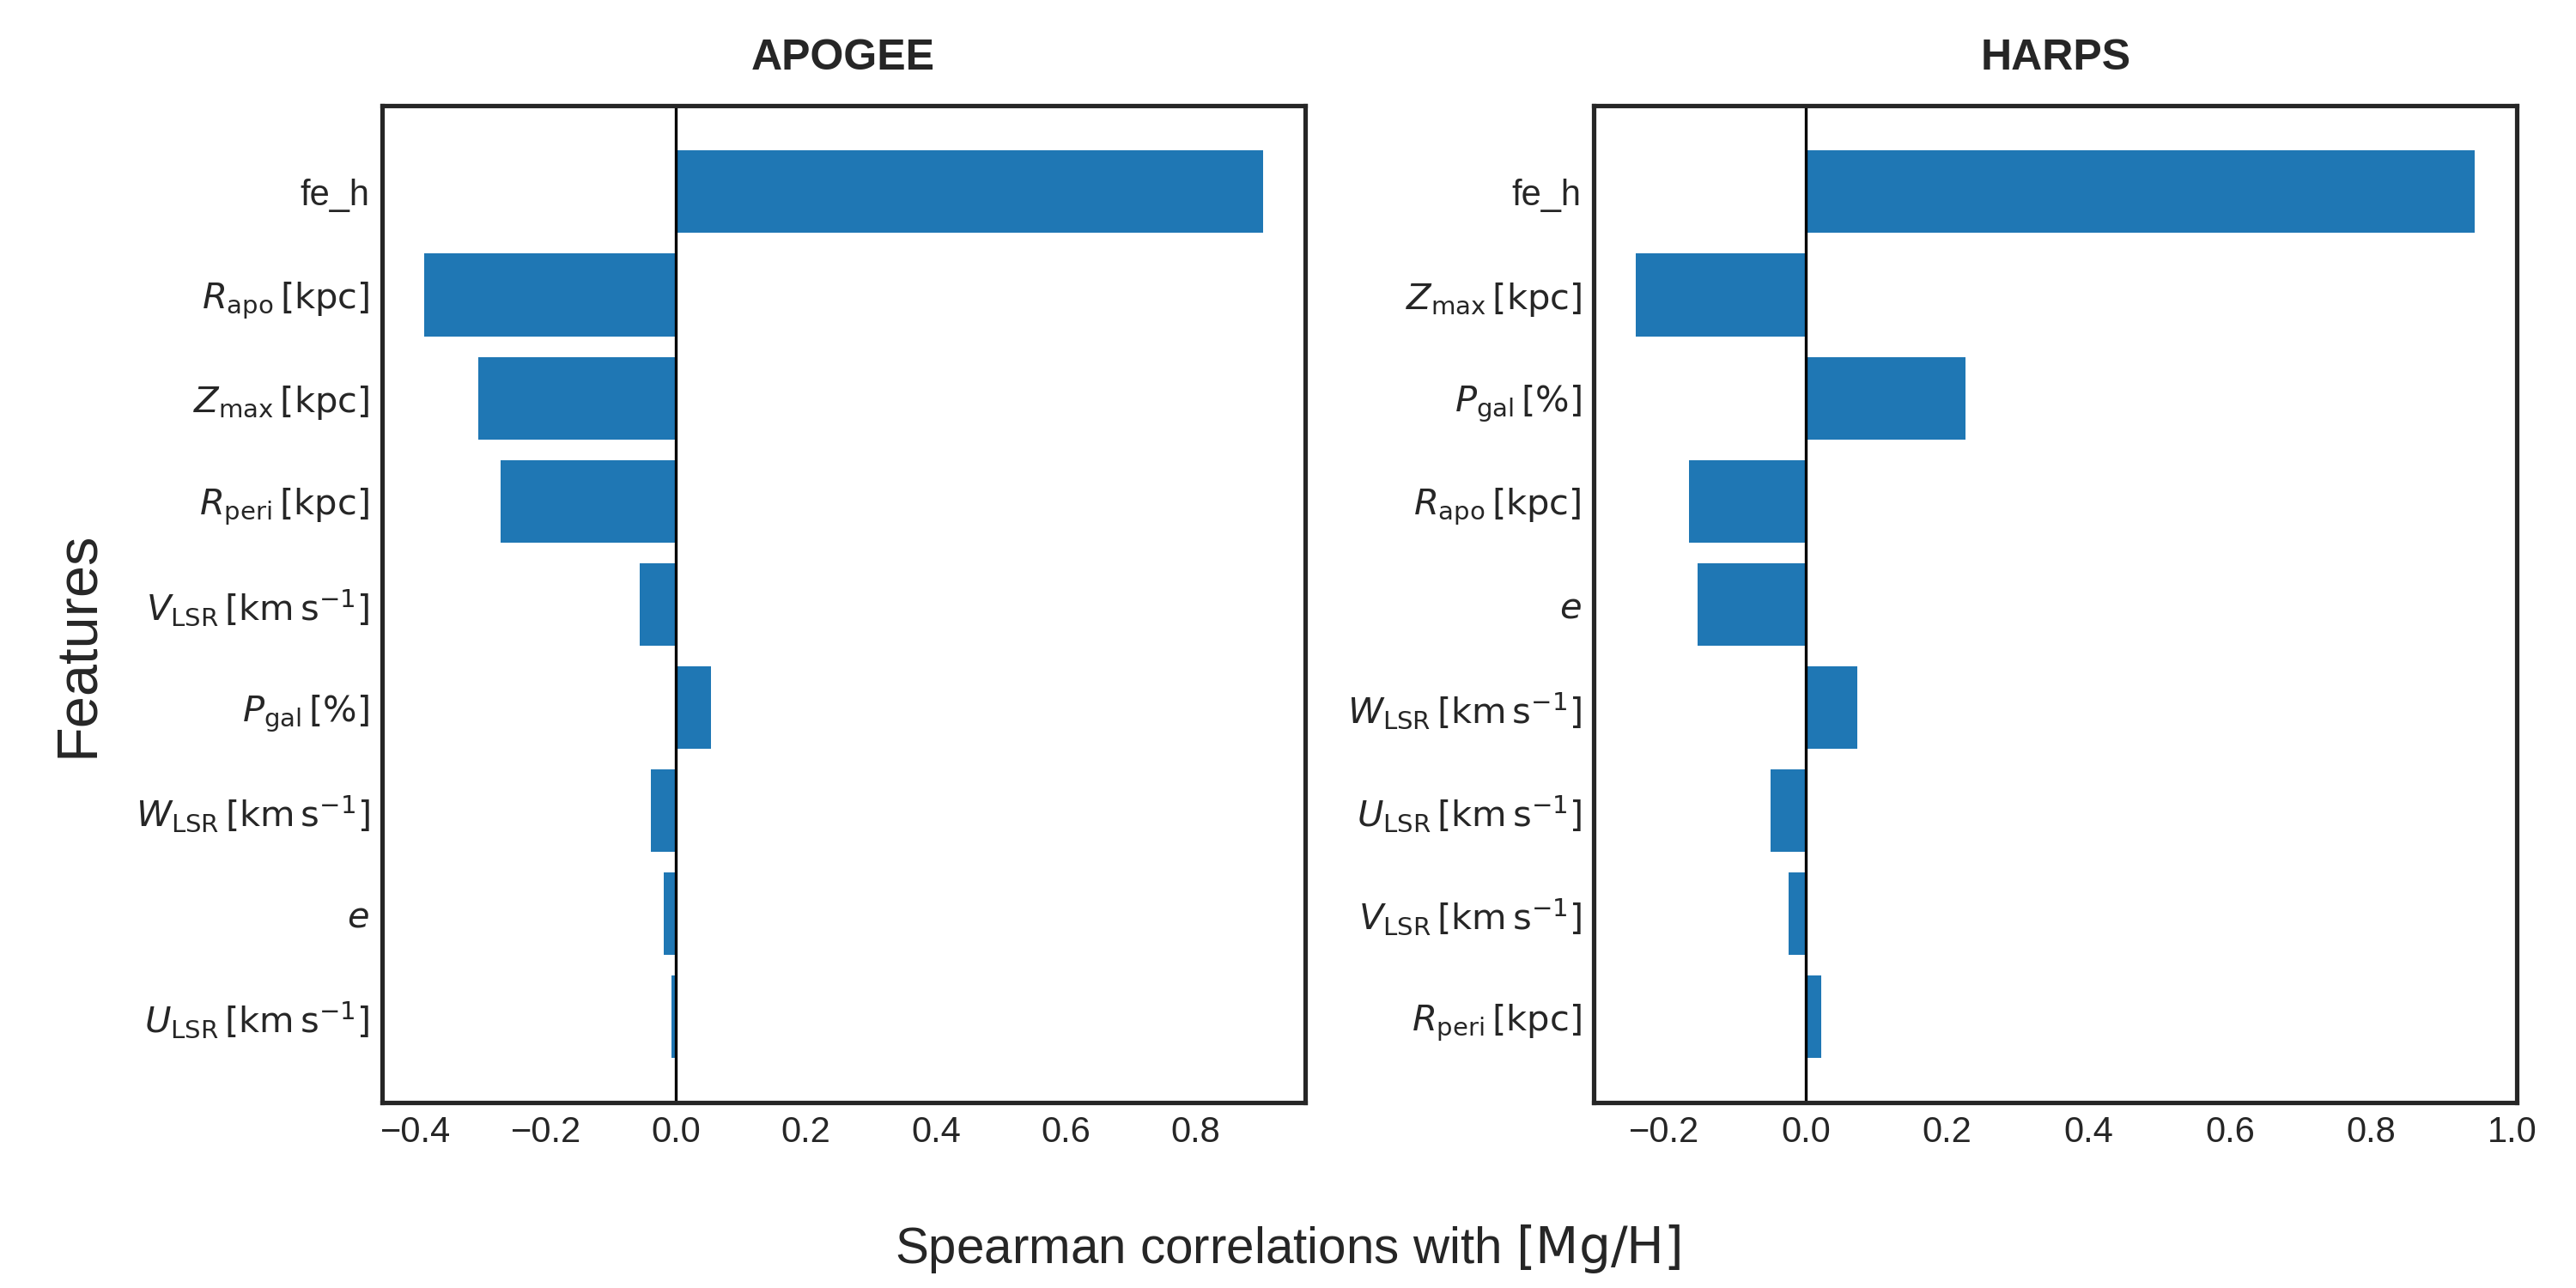
\includegraphics[width=0.48\textwidth]{figures/correlations_mg_h.png}
\vspace{0.4cm}
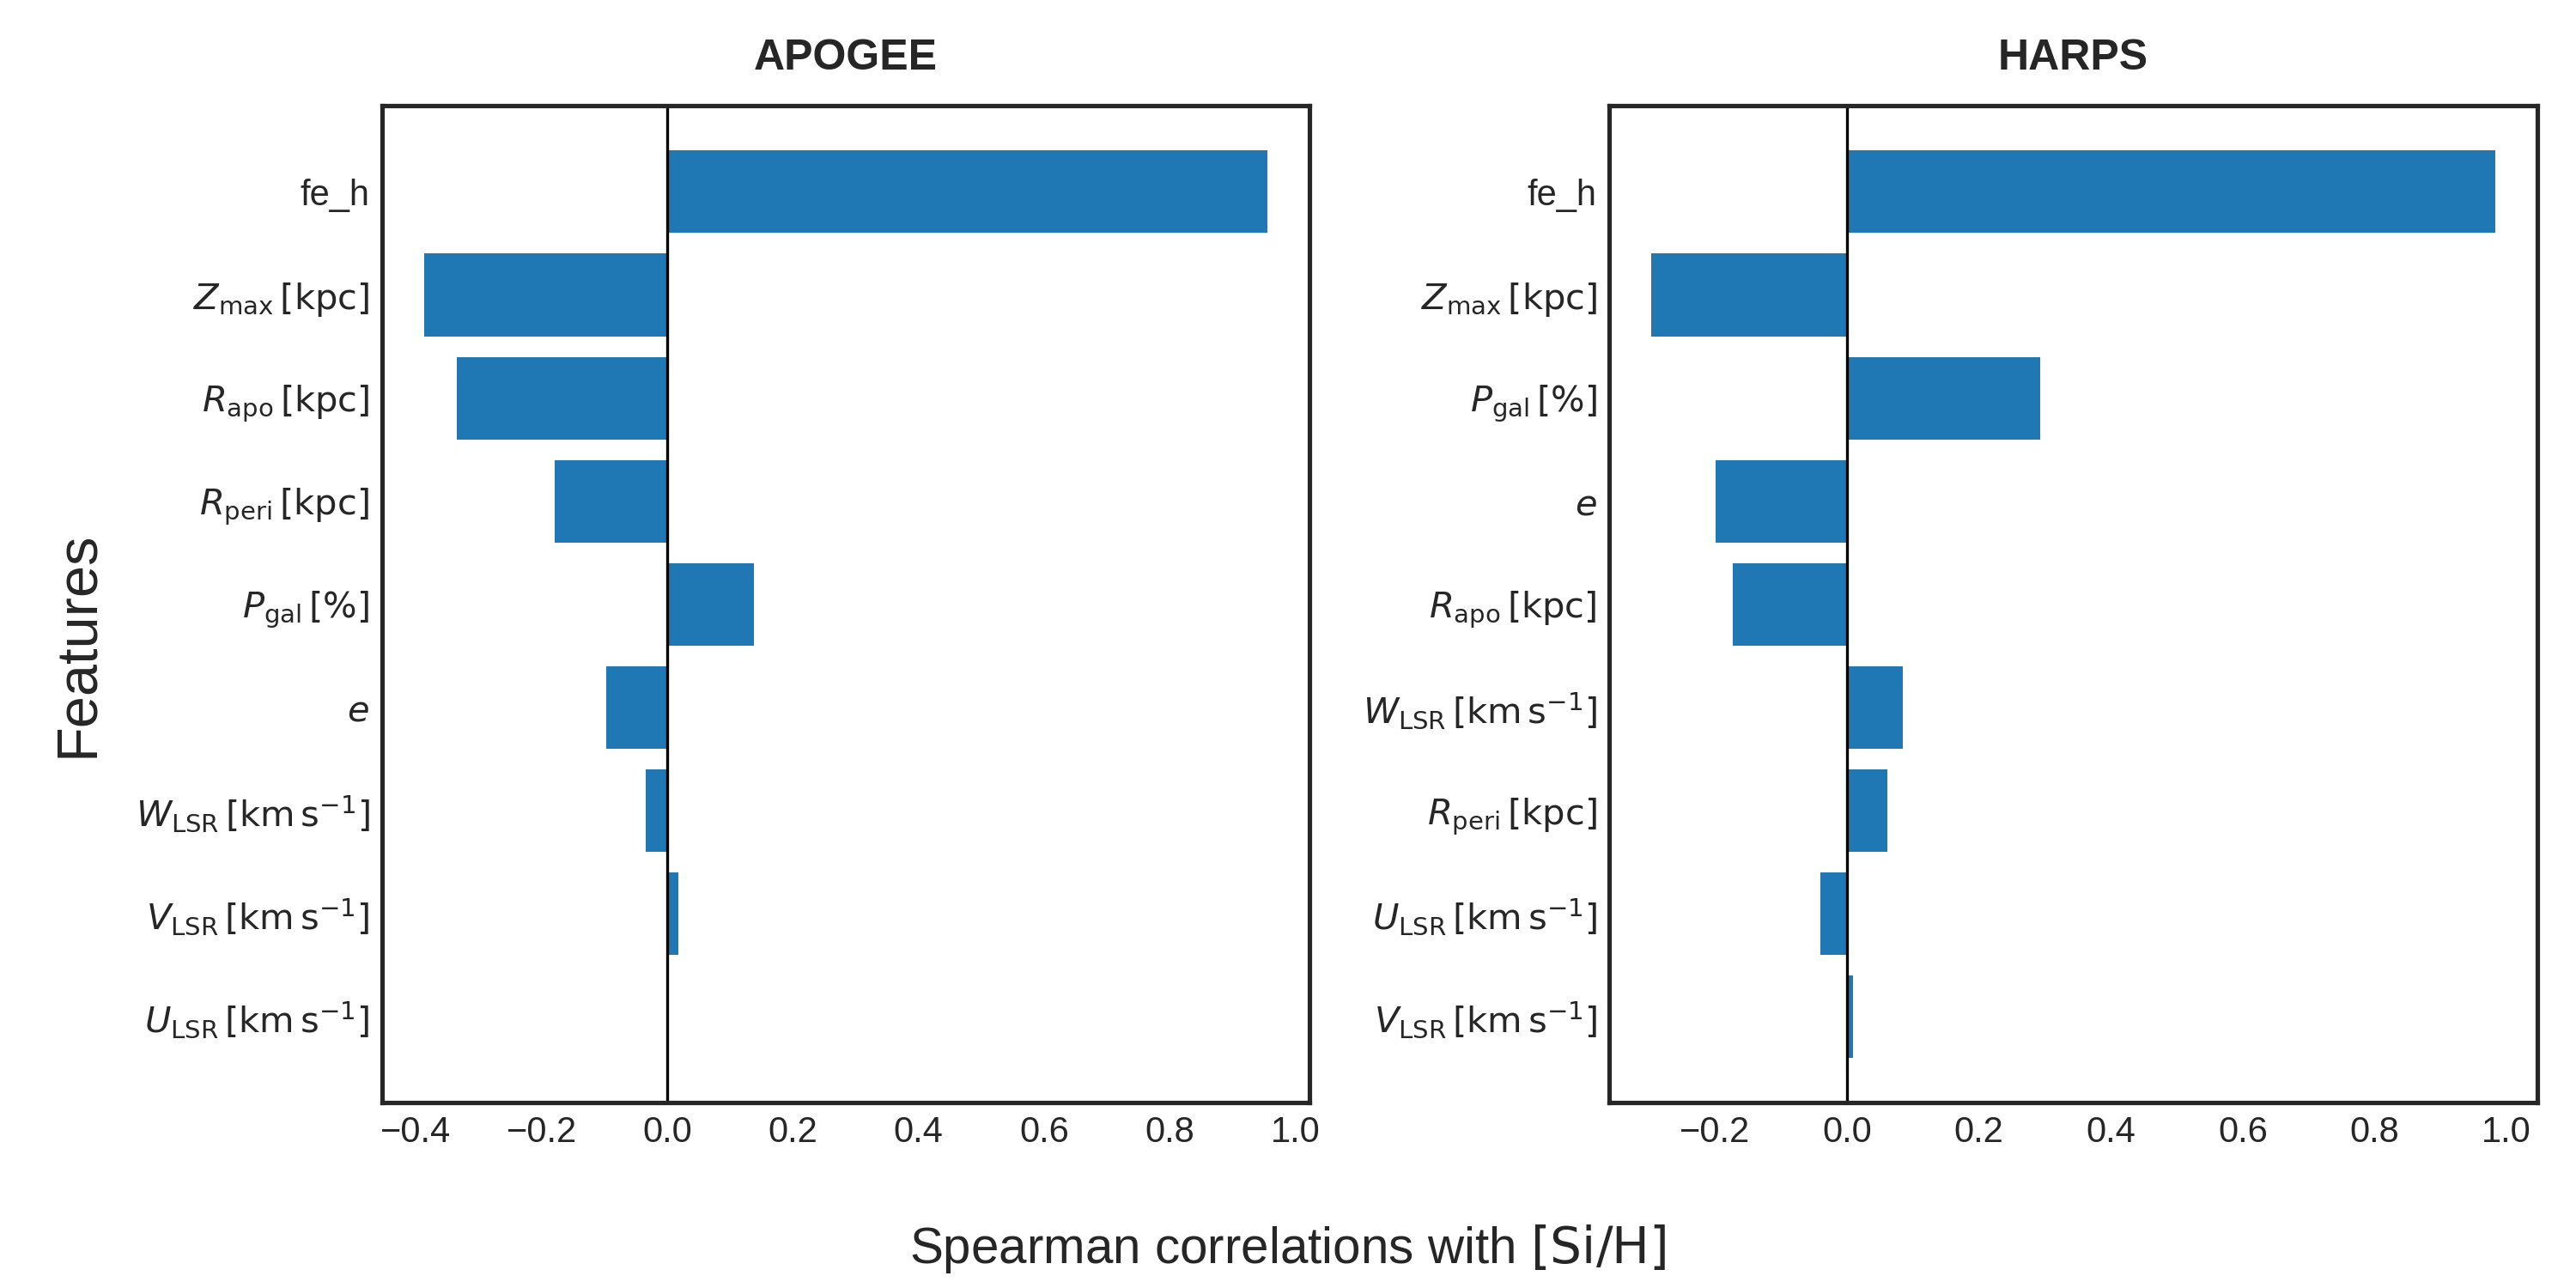
\includegraphics[width=0.48\textwidth]{figures/correlations_si_h.png}
\caption{Spearman rank correlation coefficients between the input features and the abundances of elements for the APOGEE (left) and HARPS (right) samples.}
\label{fig:cor_abund_fe}
\end{figure}


\begin{figure*}[ht]
\centering
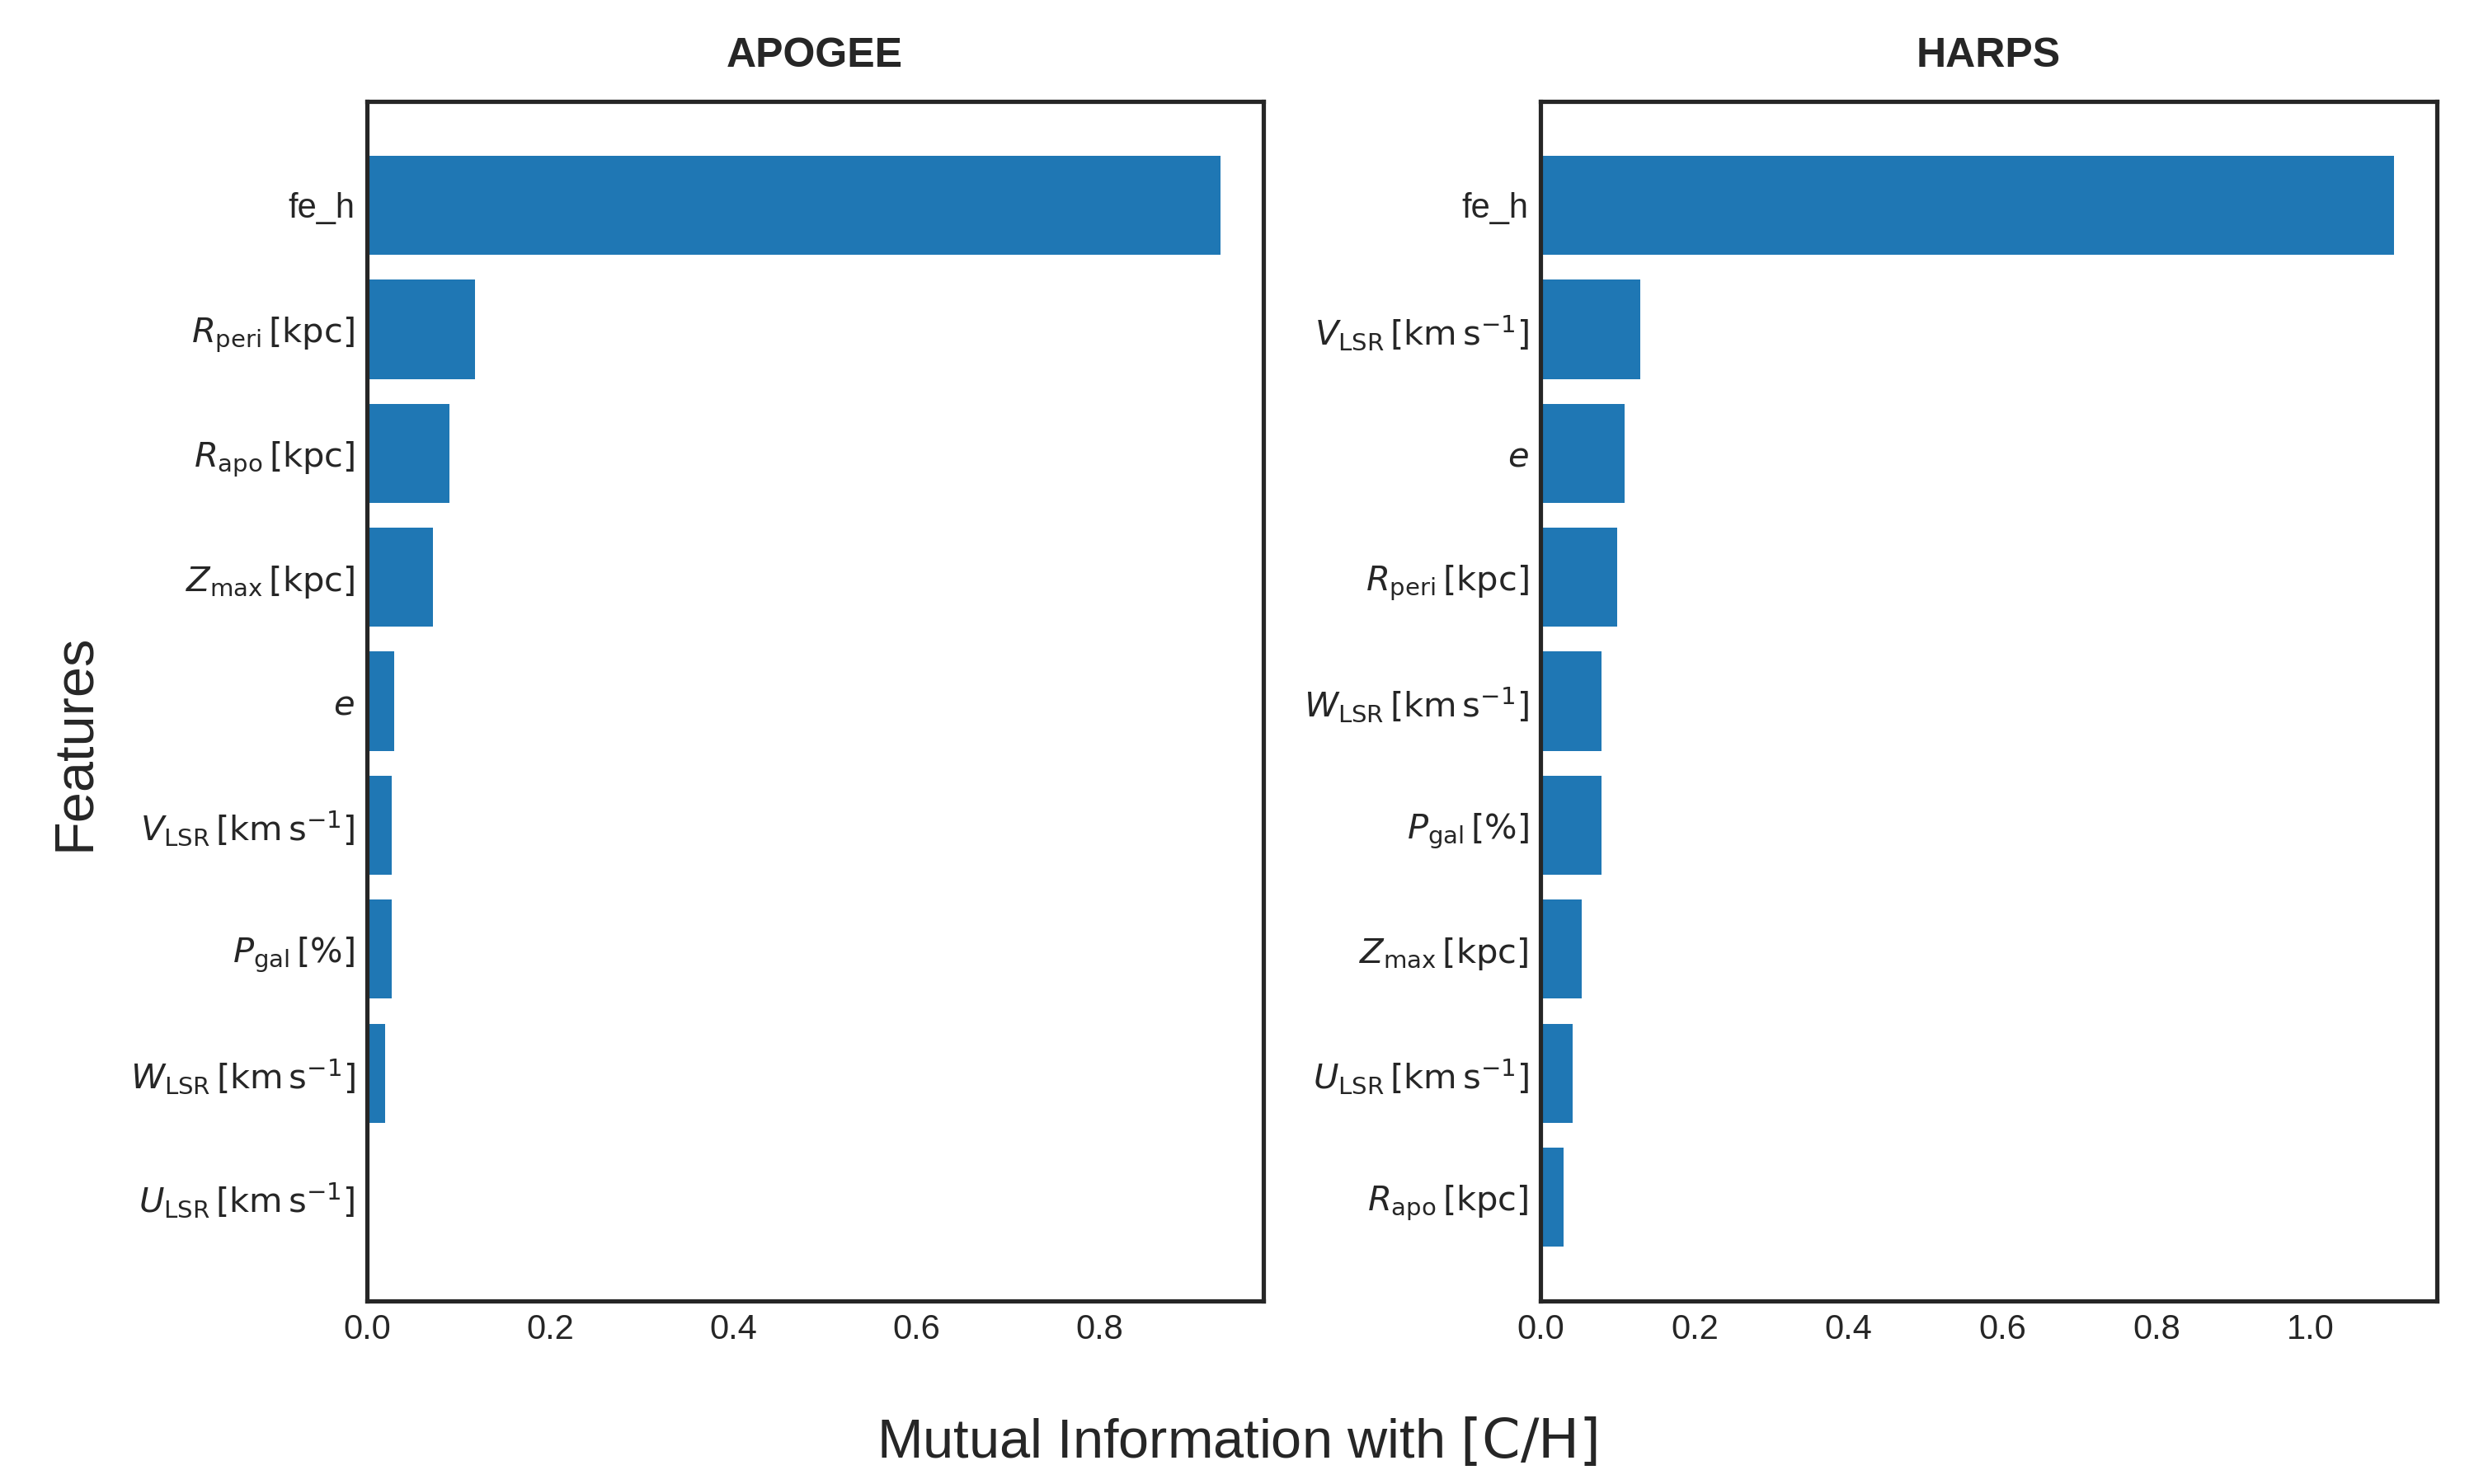
\includegraphics[width=0.48\textwidth]{figures/mi_c_h.png}
\hfill
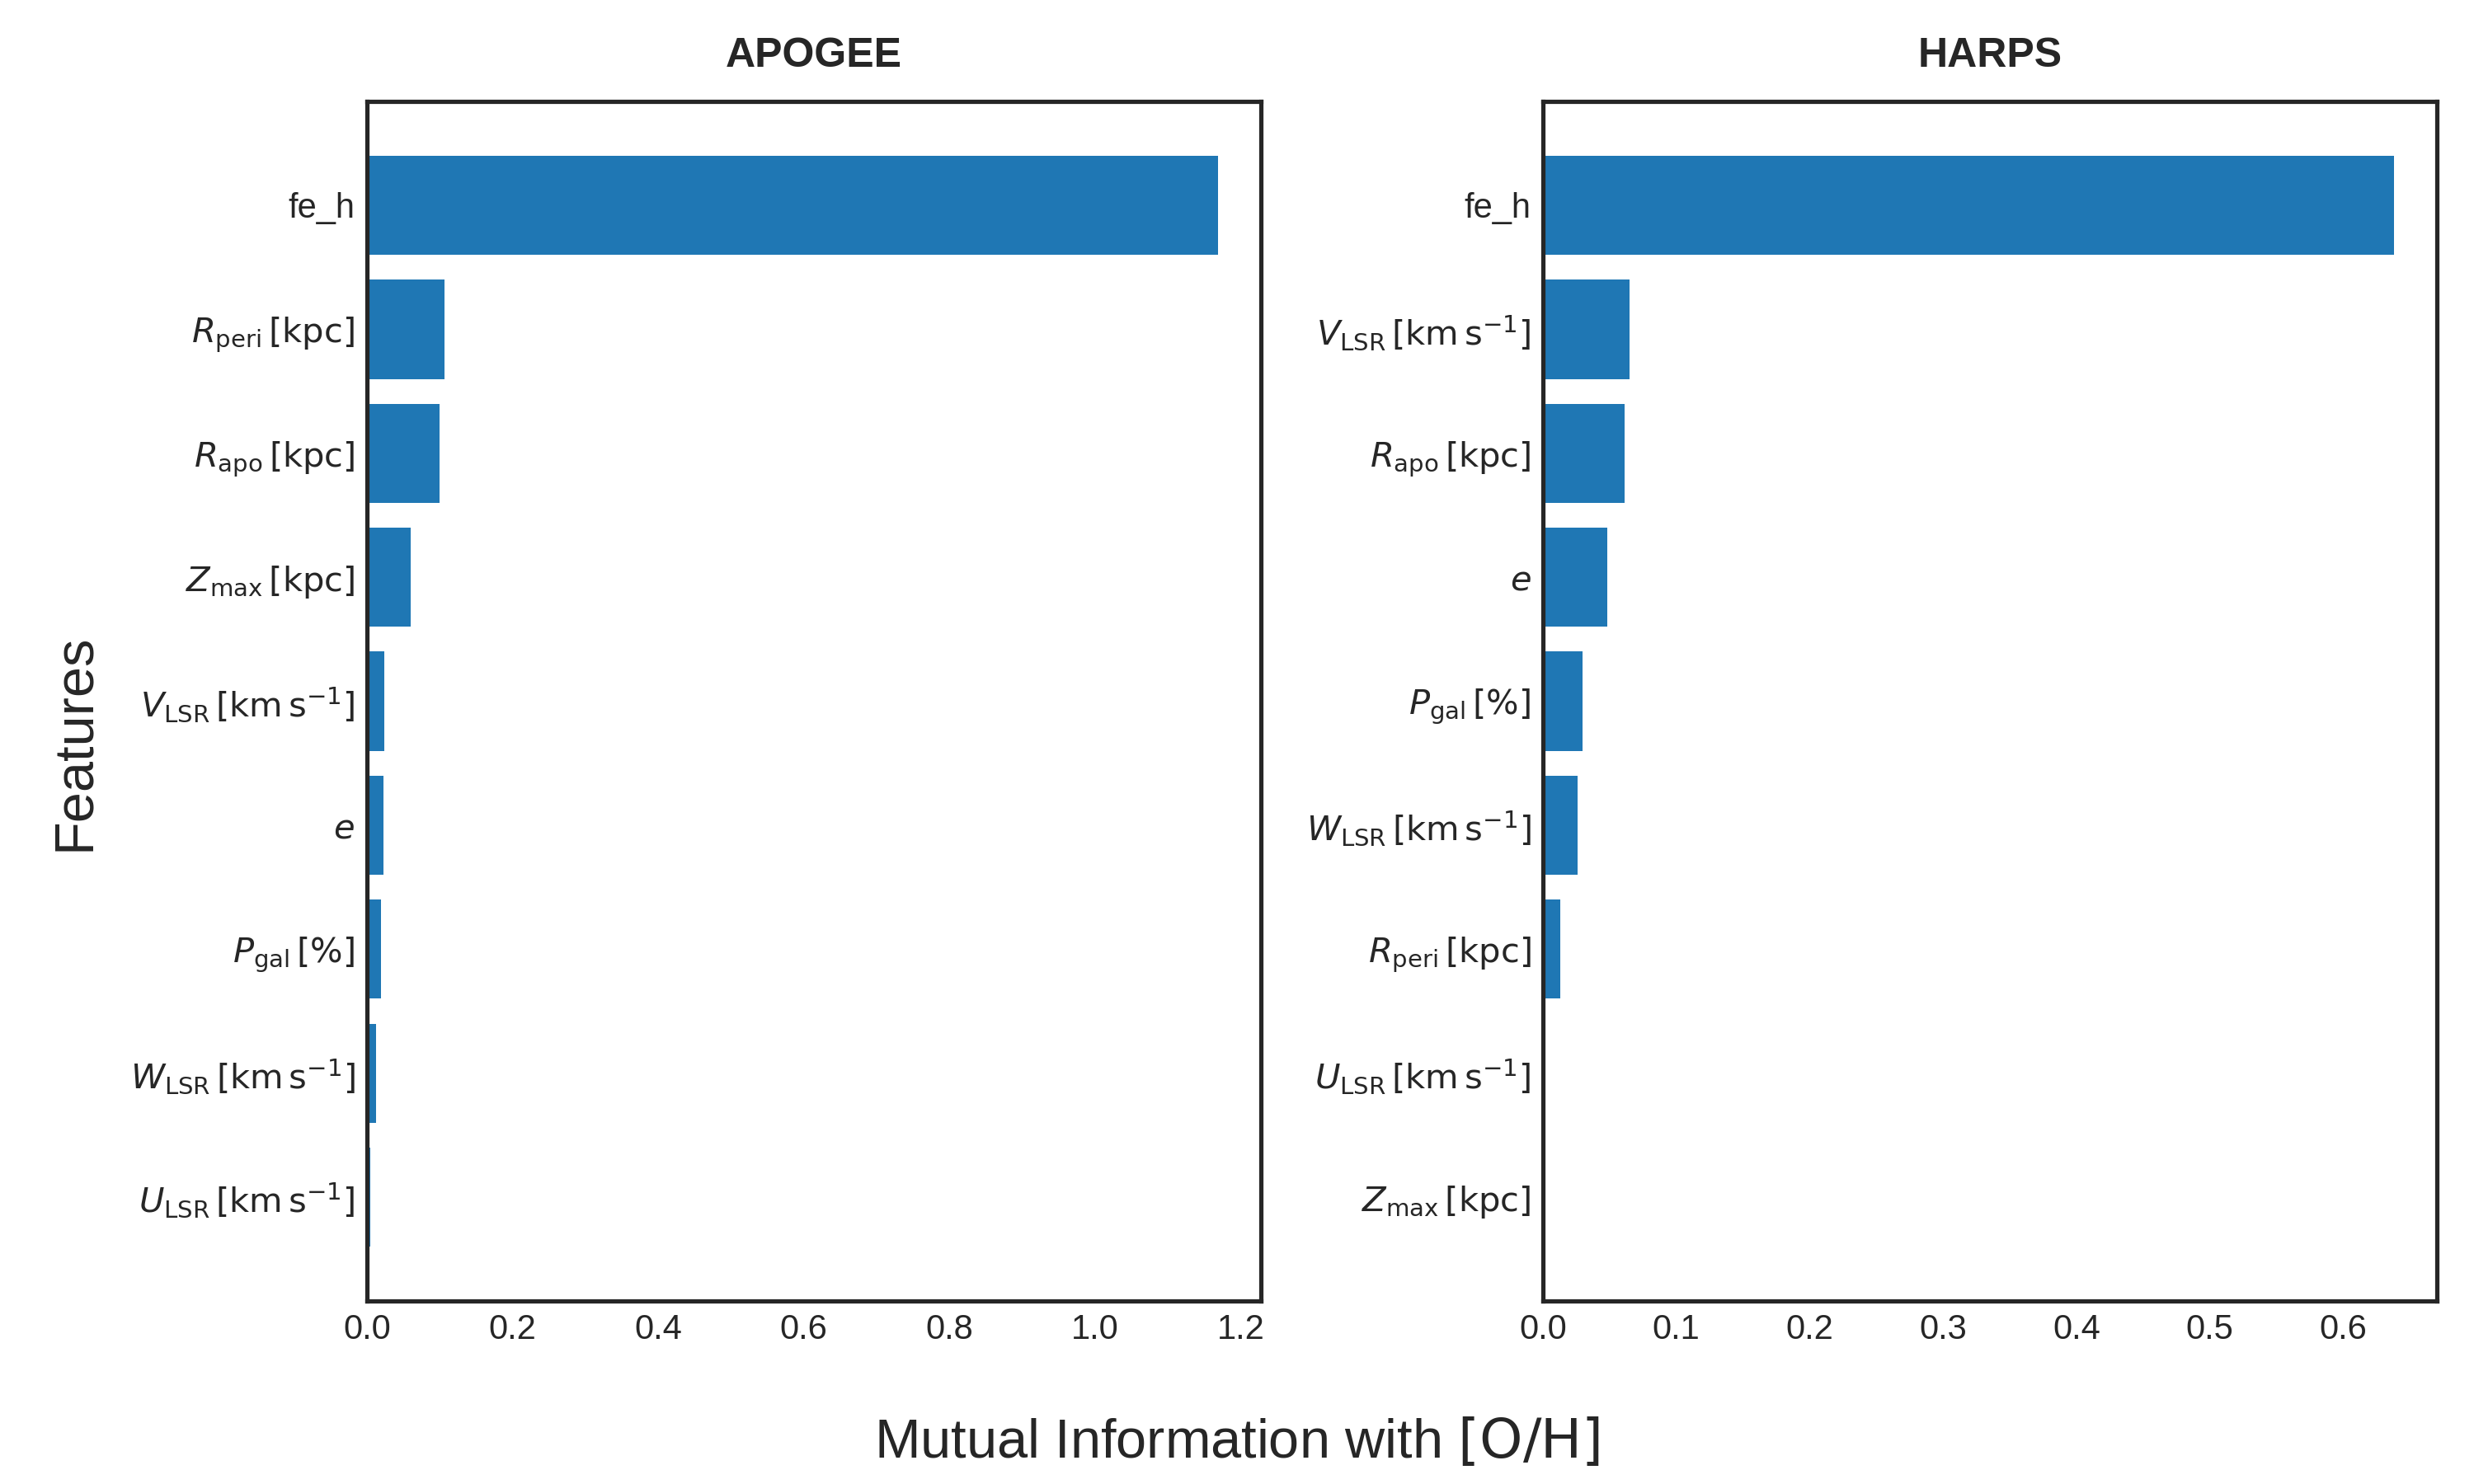
\includegraphics[width=0.48\textwidth]{figures/mi_o_h.png}
\vspace{0.4cm}
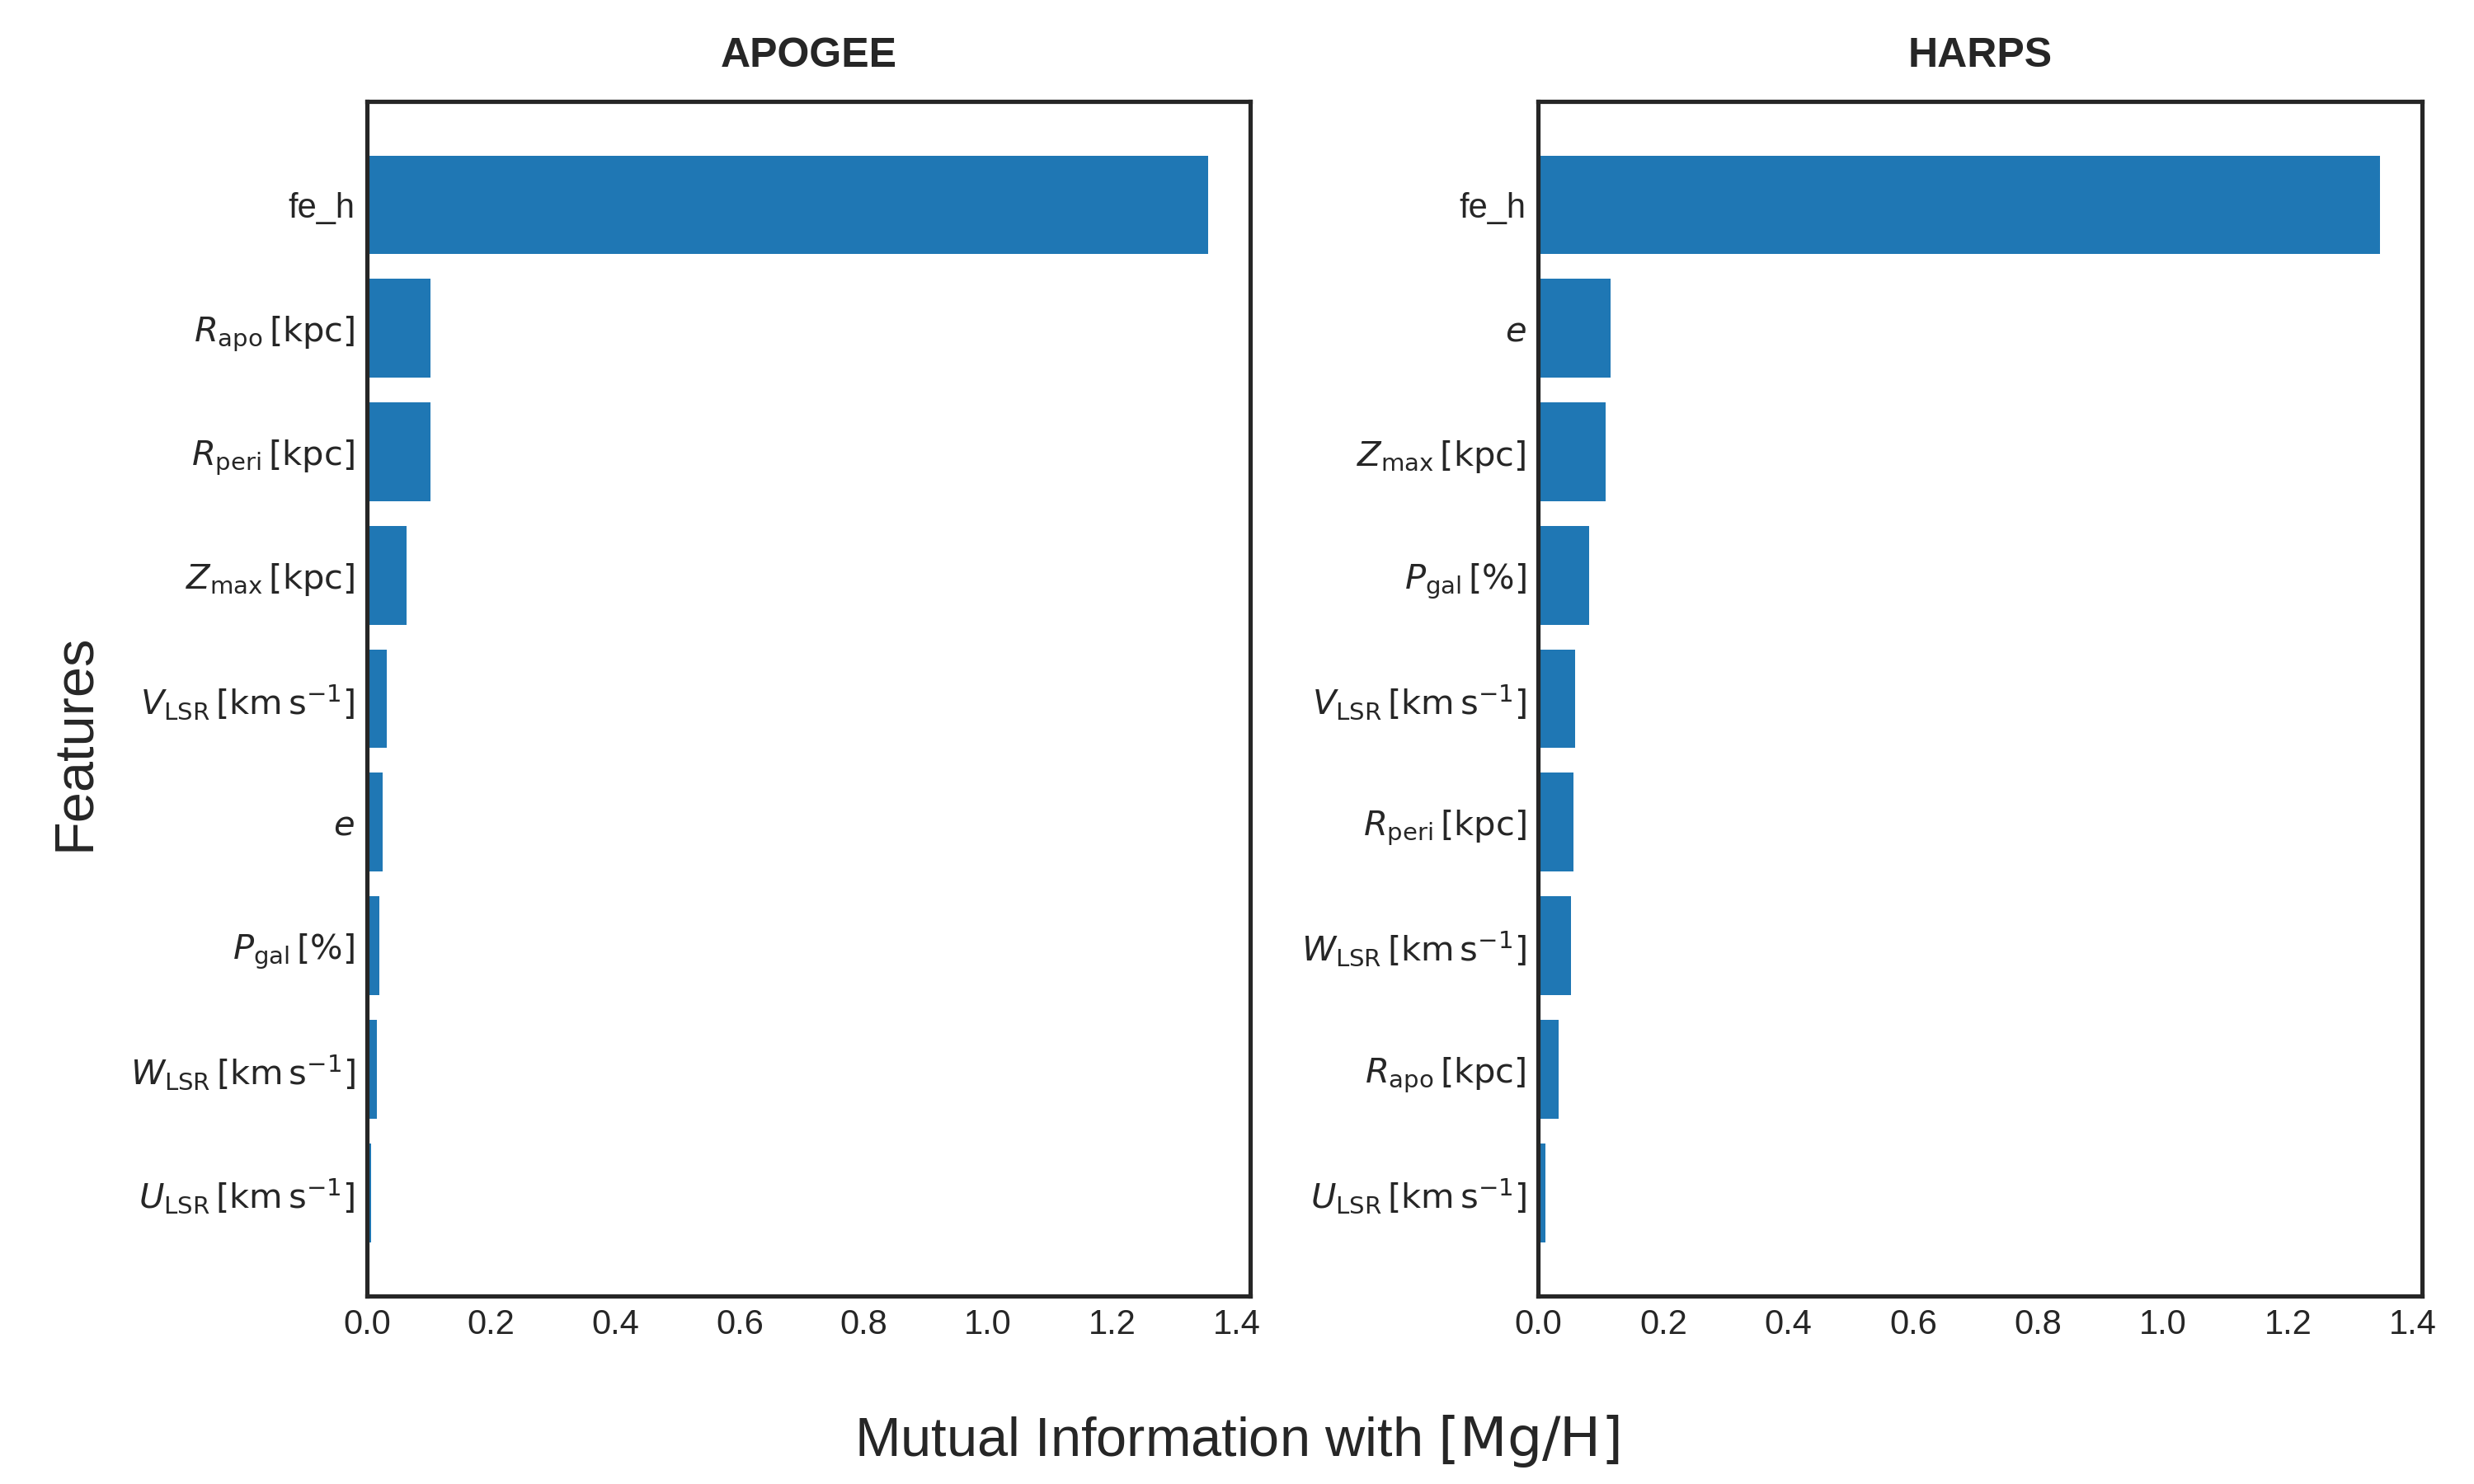
\includegraphics[width=0.48\textwidth]{figures/mi_mg_h.png}
\hfill
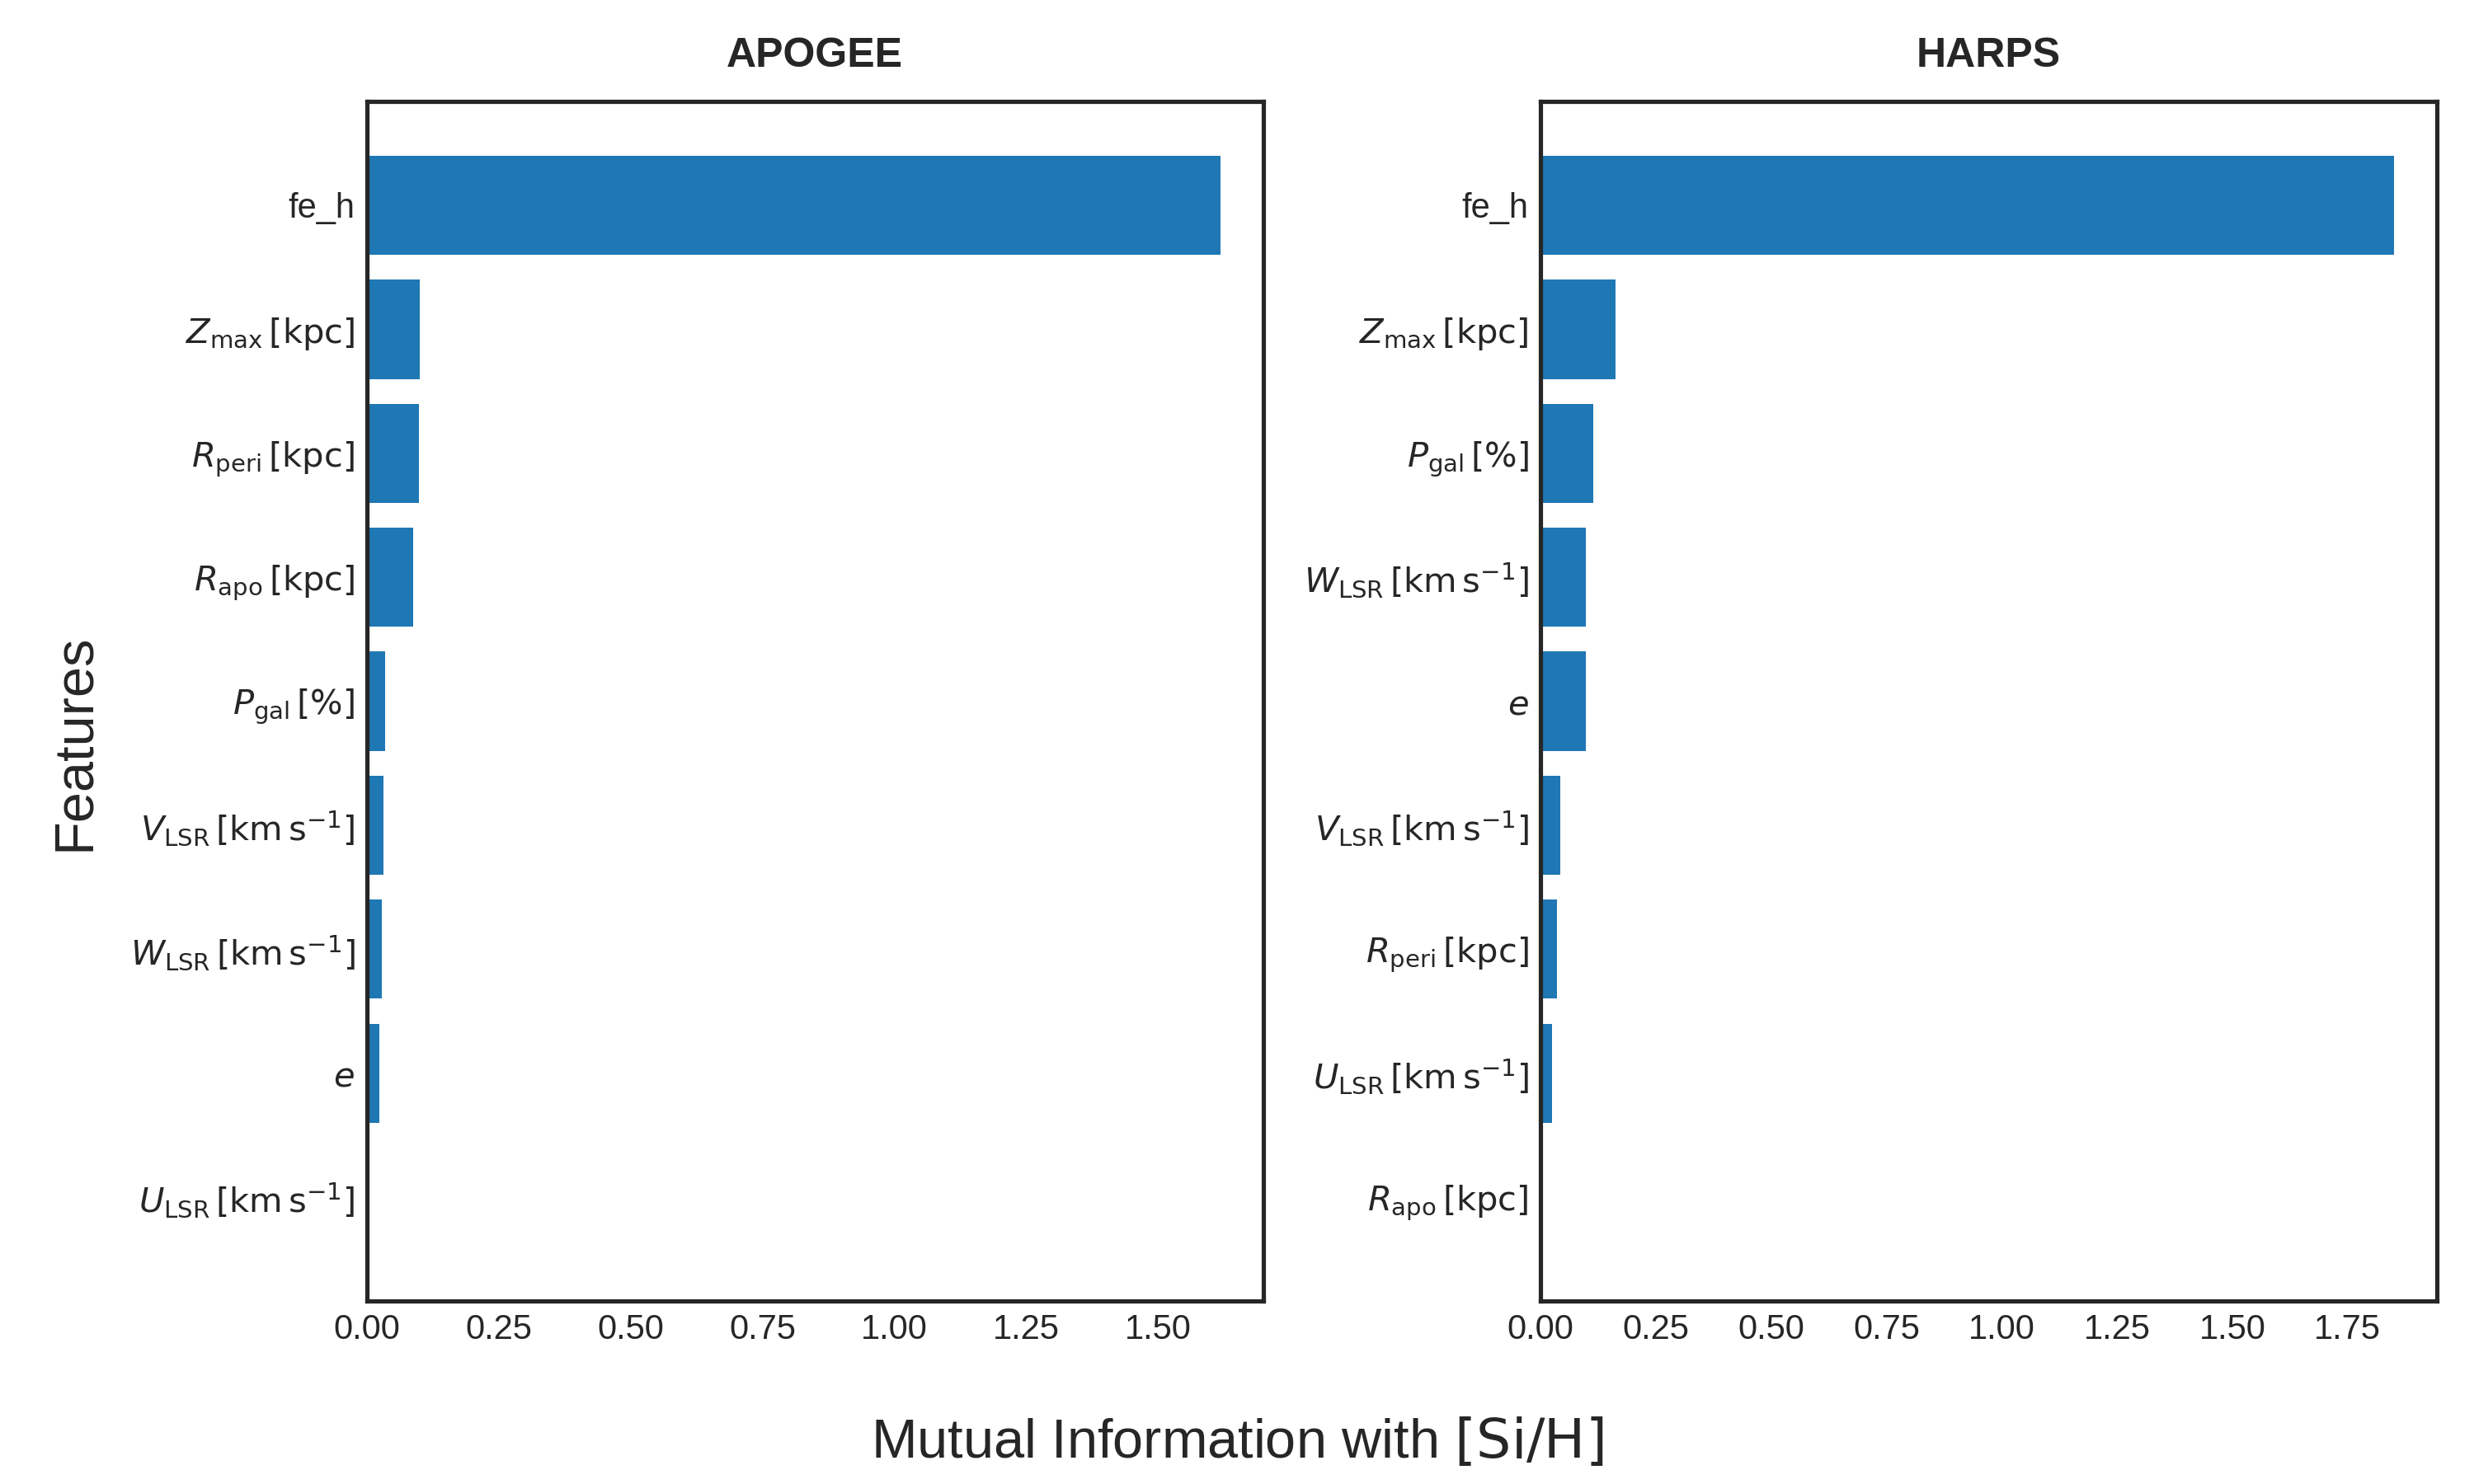
\includegraphics[width=0.48\textwidth]{figures/mi_si_h.png}
\caption{Mutual information (MI) between the input features and the abundances of elements for the APOGEE (left) and HARPS (right) samples.}
\label{fig:mi_abund_fe}
\end{figure*}




\begin{table}
\caption{Performance of regression models for predicting elemental abundances
from [Fe/H] and kinematics using five-fold cross-validation on the APOGEE
training sample. Reported values correspond to the mean across folds, with RMSE
uncertainties indicating the standard deviation.}
\centering
\begin{tabular}{lccc}
\hline
Model & RMSE (dex) & MAE (dex) & $R^2$ \\
\hline

\multicolumn{4}{l}{\textbf{[O/H]}} \\
\hline
Linear Regression & $0.061 \pm 0.000$ & 0.046 & 0.901 \\
Random Forest & $0.056 \pm 0.000$ & 0.040 & 0.916 \\
Extra Trees & $0.057 \pm 0.000$ & 0.041 & 0.914 \\
XGBoost & $0.056 \pm 0.000$ & 0.040 & 0.915 \\
XGBoost (QT) & $0.057 \pm 0.001$ & 0.040 & 0.914 \\
LightGBM & $\mathbf{0.055 \pm 0.000}$ & 0.039 & 0.920 \\
LightGBM (QT) & $0.055 \pm 0.000$ & 0.039 & 0.919 \\
CatBoost & $0.055 \pm 0.001$ & 0.039 & 0.920 \\
CatBoost (QT) & $0.055 \pm 0.001$ & 0.039 & 0.919 \\
Voting Regressor & $0.055 \pm 0.000$ & 0.039 & 0.920 \\
\hline


\multicolumn{4}{l}{\textbf{[Mg/H]}} \\
\hline
Linear Regression & $0.057 \pm 0.000$ & 0.044 & 0.920 \\
Random Forest & $0.051 \pm 0.000$ & 0.037 & 0.937 \\
Extra Trees & $0.051 \pm 0.000$ & 0.037 & 0.937 \\
XGBoost & $0.051 \pm 0.000$ & 0.036 & 0.938 \\
XGBoost (QT) & $0.051 \pm 0.000$ & 0.036 & 0.937 \\
LightGBM & $\mathbf{0.049 \pm 0.001}$ & 0.035 & 0.941 \\
LightGBM (QT) & $0.049 \pm 0.001$ & 0.035 & 0.941 \\
CatBoost & $0.049 \pm 0.000$ & 0.035 & 0.941 \\
CatBoost (QT) & $0.049 \pm 0.000$ & 0.035 & 0.941 \\
Voting Regressor & $0.049 \pm 0.000$ & 0.035 & 0.941 \\
\hline

\multicolumn{4}{l}{\textbf{[Si/H]}} \\
\hline
Linear Regression & $0.041 \pm 0.000$ & 0.032 & 0.961 \\
Random Forest & $0.038 \pm 0.000$ & 0.028 & 0.967 \\
Extra Trees & $0.038 \pm 0.000$ & 0.028 & 0.967 \\
XGBoost & $0.038 \pm 0.000$ & 0.028 & 0.968 \\
XGBoost (QT) & $0.038 \pm 0.000$ & 0.028 & 0.967 \\
LightGBM & $\mathbf{0.037 \pm 0.000}$ & 0.027 & 0.969 \\
LightGBM (QT) & $0.037 \pm 0.000$ & 0.027 & 0.969 \\
CatBoost & $0.037 \pm 0.000$ & 0.027 & 0.969 \\
CatBoost (QT) & $0.037 \pm 0.000$ & 0.027 & 0.969 \\
Voting Regressor & $0.037 \pm 0.000$ & 0.027 & 0.969 \\
\hline

\multicolumn{4}{l}{\textbf{[C/H]}} \\
\hline
Linear Regression & $0.086 \pm 0.000$ & 0.065 & 0.872 \\
Random Forest & $0.081 \pm 0.001$ & 0.060 & 0.887 \\
Extra Trees & $0.082 \pm 0.000$ & 0.061 & 0.885 \\
XGBoost & $0.081 \pm 0.001$ & 0.060 & 0.888 \\
XGBoost (QT) & $0.081 \pm 0.001$ & 0.060 & 0.886 \\
LightGBM & $\mathbf{0.079 \pm 0.001}$ & 0.058 & 0.893 \\
LightGBM (QT) & $0.079 \pm 0.001$ & 0.058 & 0.893 \\
CatBoost & $0.079 \pm 0.001$ & 0.058 & 0.893 \\
CatBoost (QT) & $0.079 \pm 0.001$ & 0.059 & 0.892 \\
Voting Regressor & $0.079 \pm 0.001$ & 0.059 & 0.892 \\
\hline


\end{tabular}
\label{tab:abundance_cv_scores}
\end{table}


\subsubsection{Feature importance analysis} \label{appendix:feature_importance_abundances_feh}


This appendix presents the full set of feature-importance figures discussed in Sect.\ref{main_feat_imp_abund_feh} For completeness, we show the results of the built-in gain importance, permutation importance, SHAP global importance, and single-feature predictive performance for the LightGBM model.

\begin{figure*}[ht]
\centering
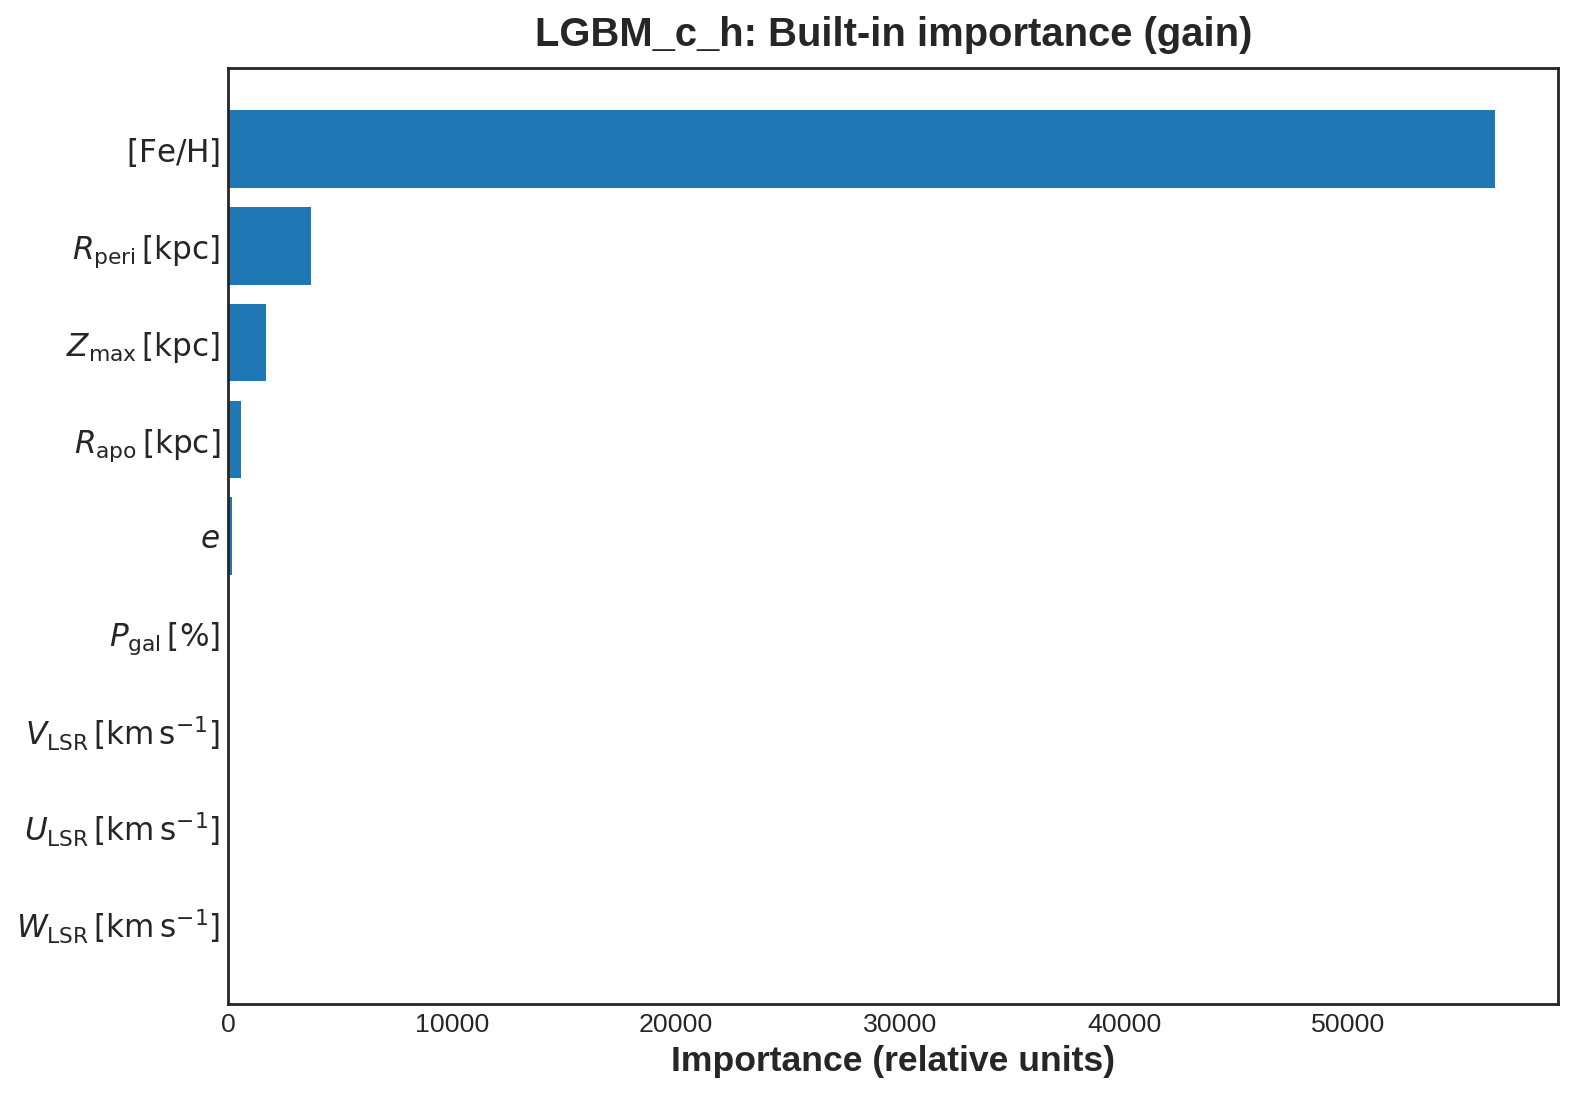
\includegraphics[width=0.24\textwidth]{figures/LGBM_c_h_builtin_gain.png}
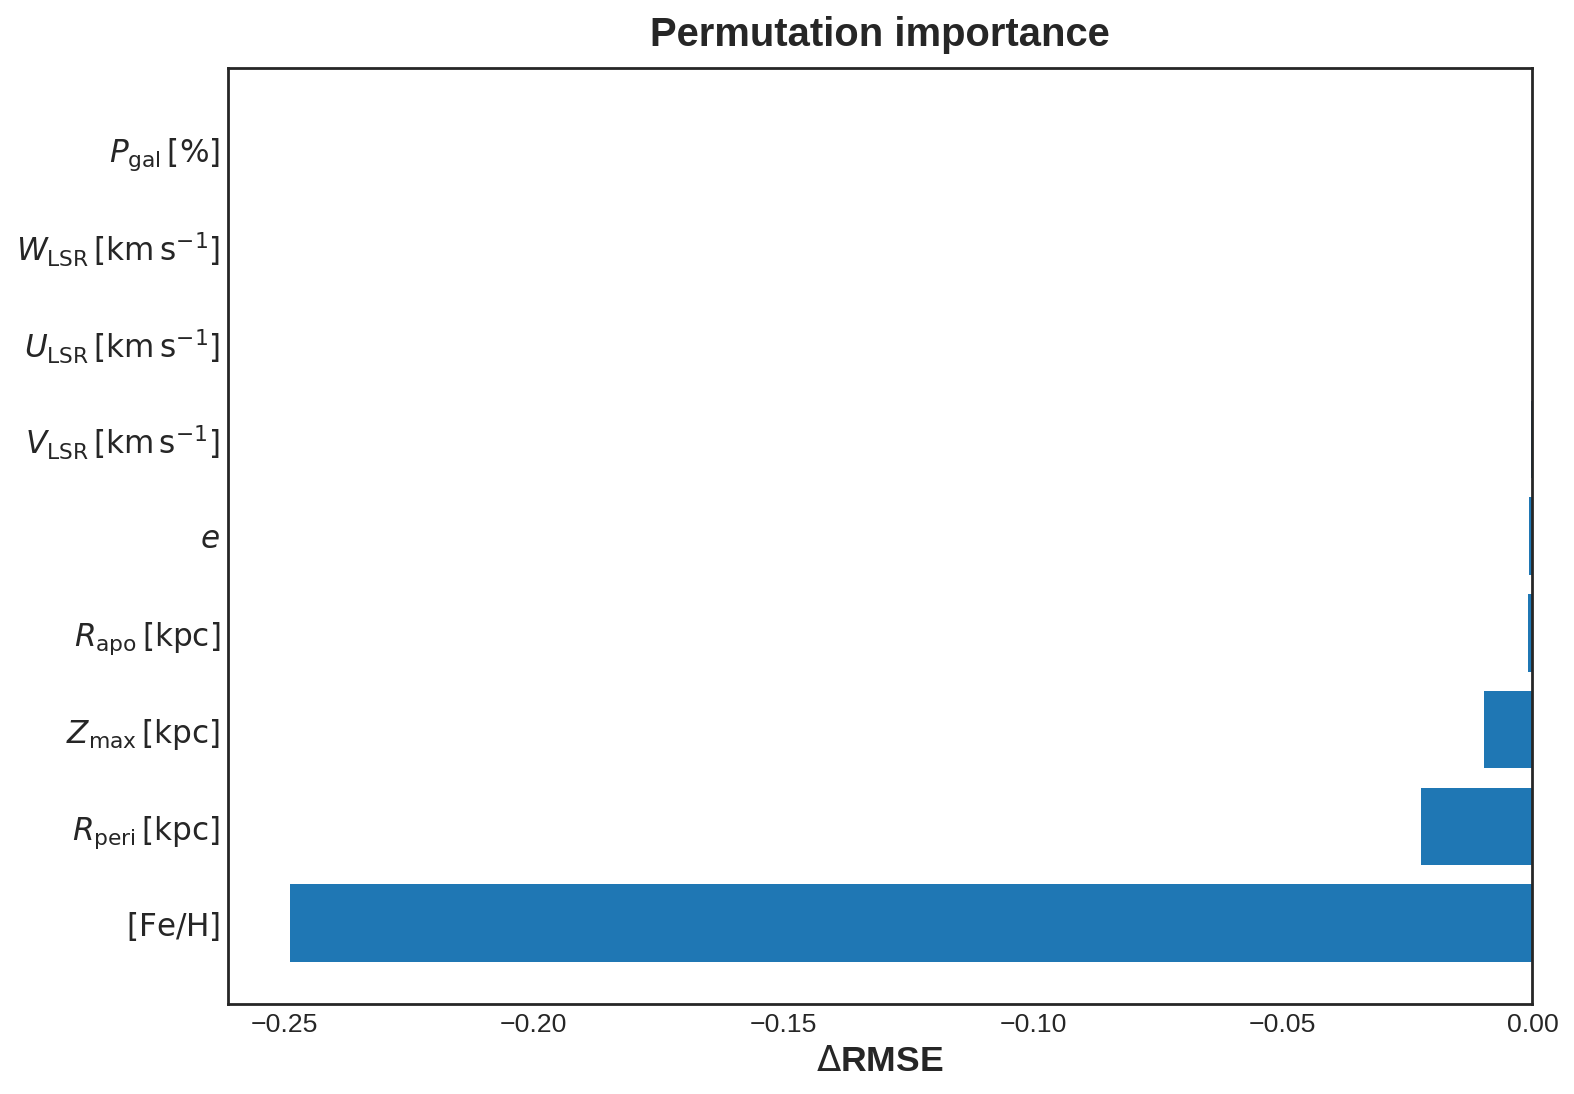
\includegraphics[width=0.24\textwidth]{figures/LGBM_c_h_permutation_dRMSE.png}
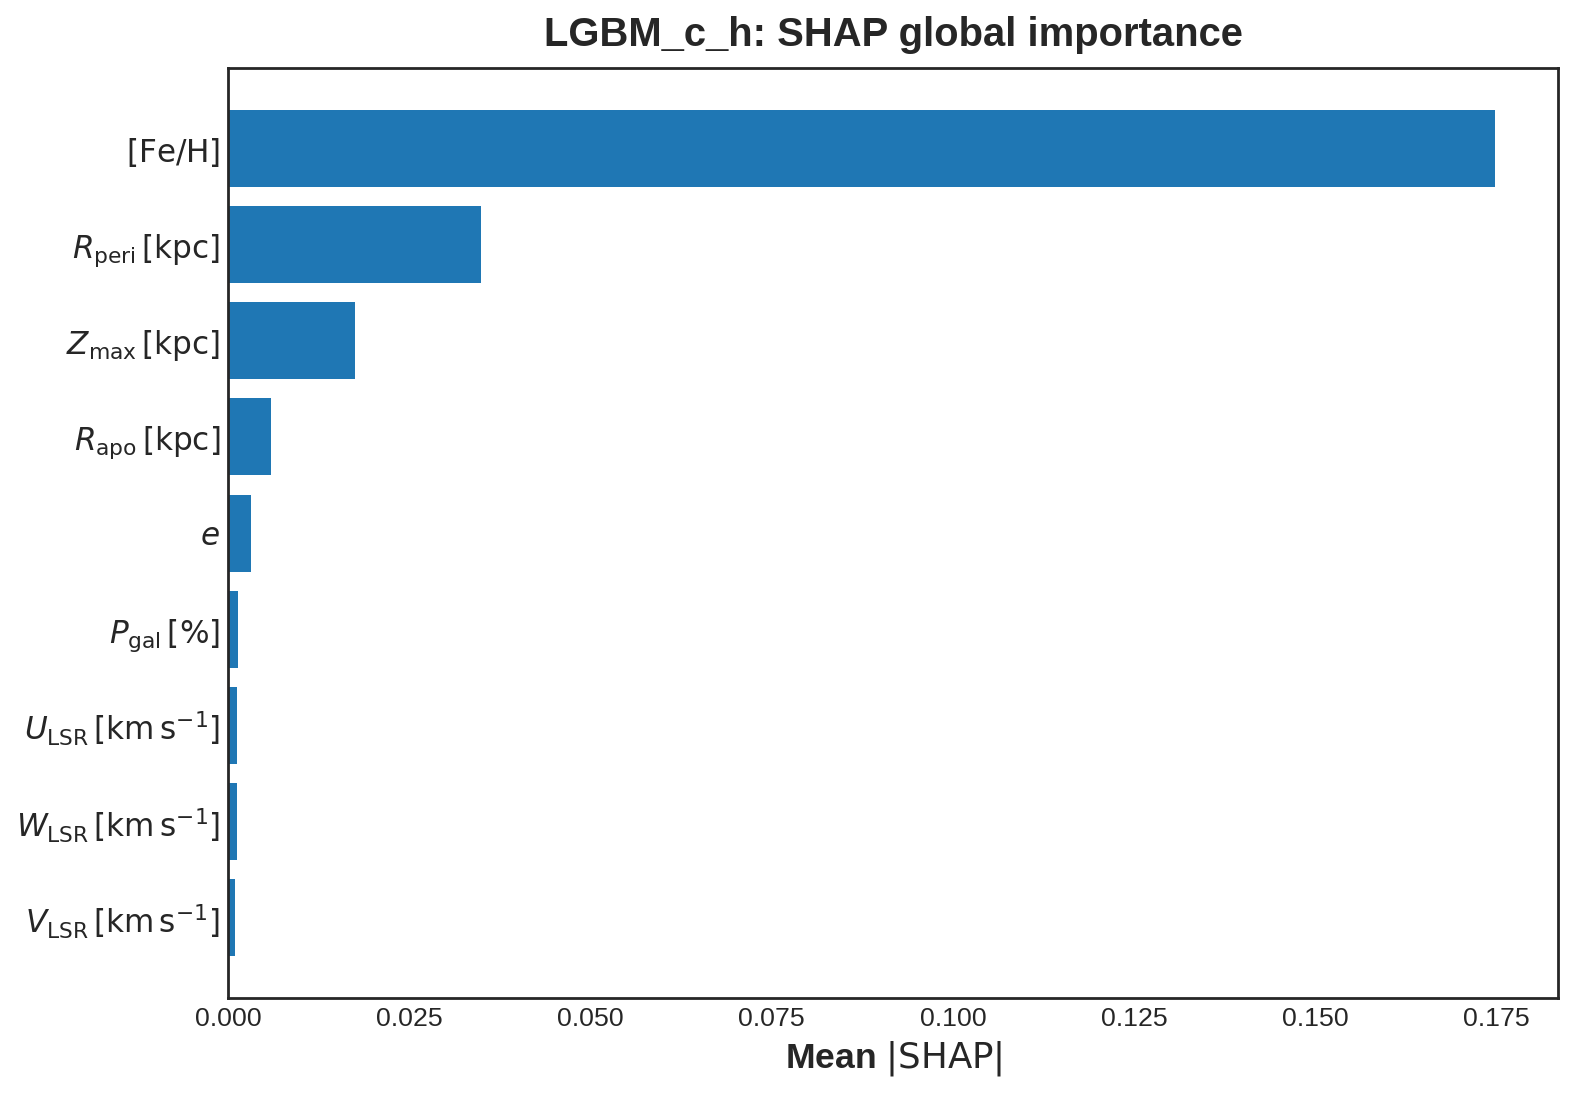
\includegraphics[width=0.24\textwidth]{figures/LGBM_c_h_shap_meanabs.png}
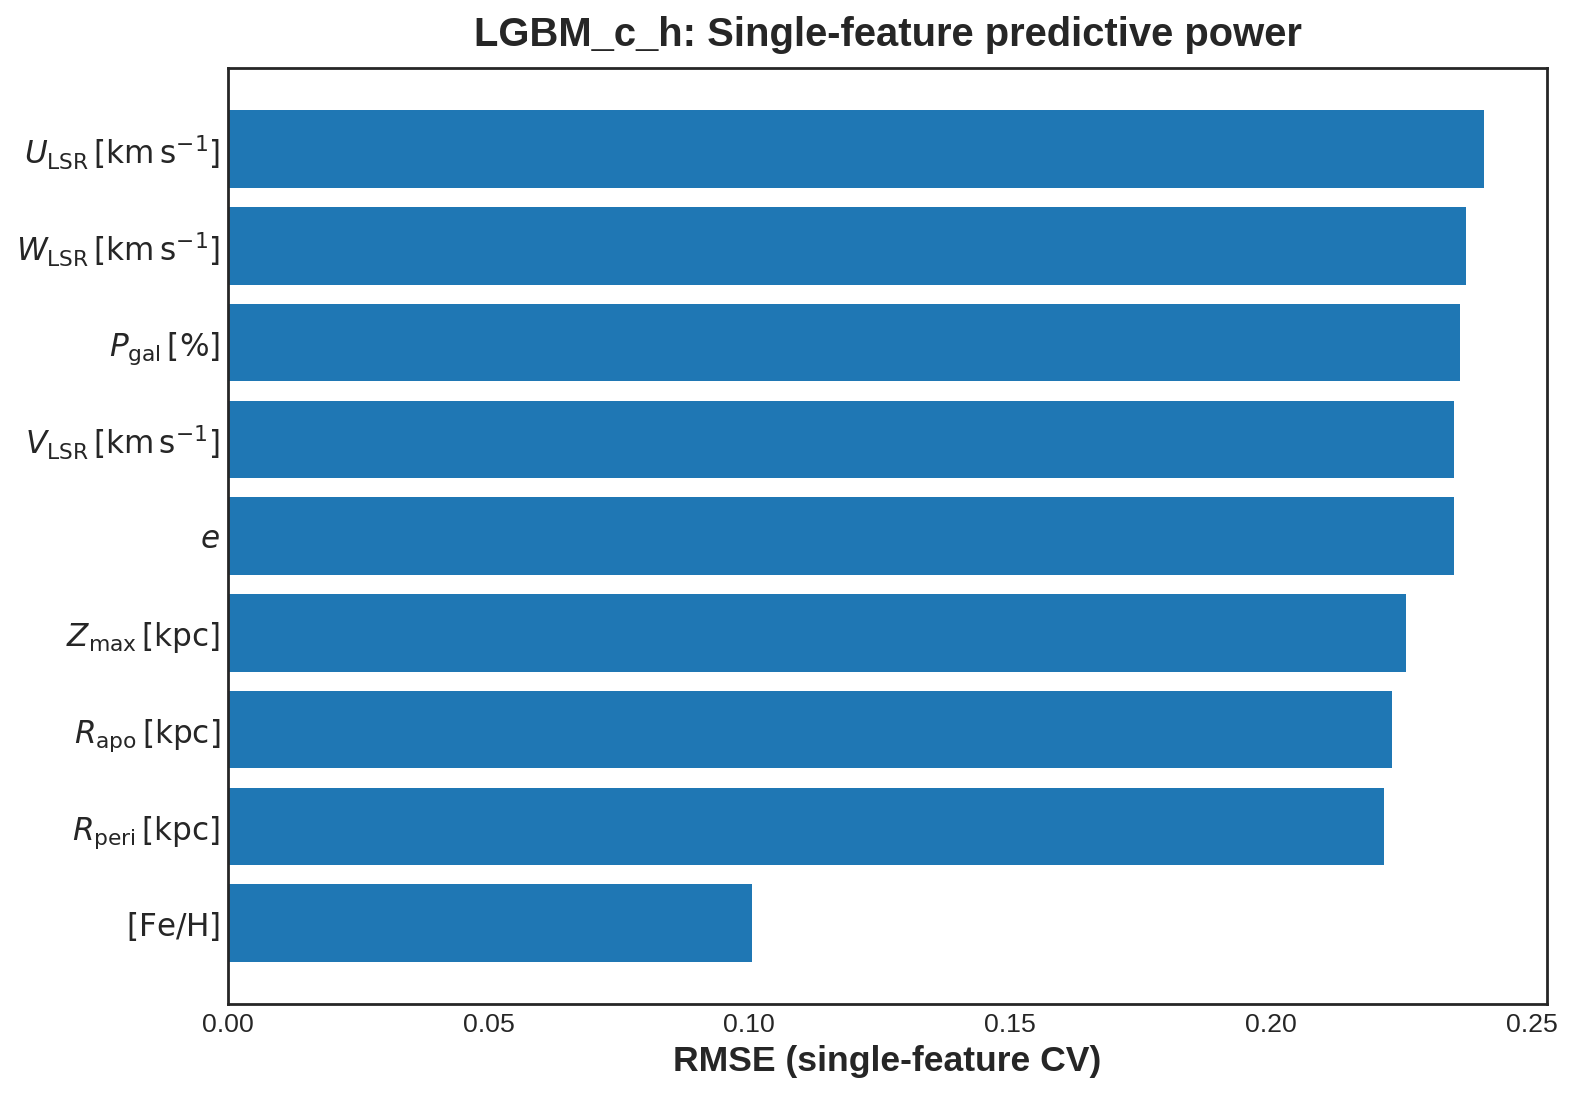
\includegraphics[width=0.24\textwidth]{figures/LGBM_c_h_single_feature_rmse.png}
\caption{
Feature-importance diagnostics for the tuned LightGBM model predicting $\mathrm{[C/H]}$. Built-in gain feature importance derived from the gradient boosting trees (top left). Permutation feature importance, measured as the increase in prediction error ($\Delta$RMSE) after randomly shuffling each feature (top right). Global SHAP importance, showing the mean absolute SHAP value for each feature (bottom left). Predictive performance (RMSE from cross-validation) obtained when training the model using only a single feature at a time (bottom right).}
\label{fig:feature_importance_ch}
\end{figure*}


\begin{figure*}[ht]
\centering
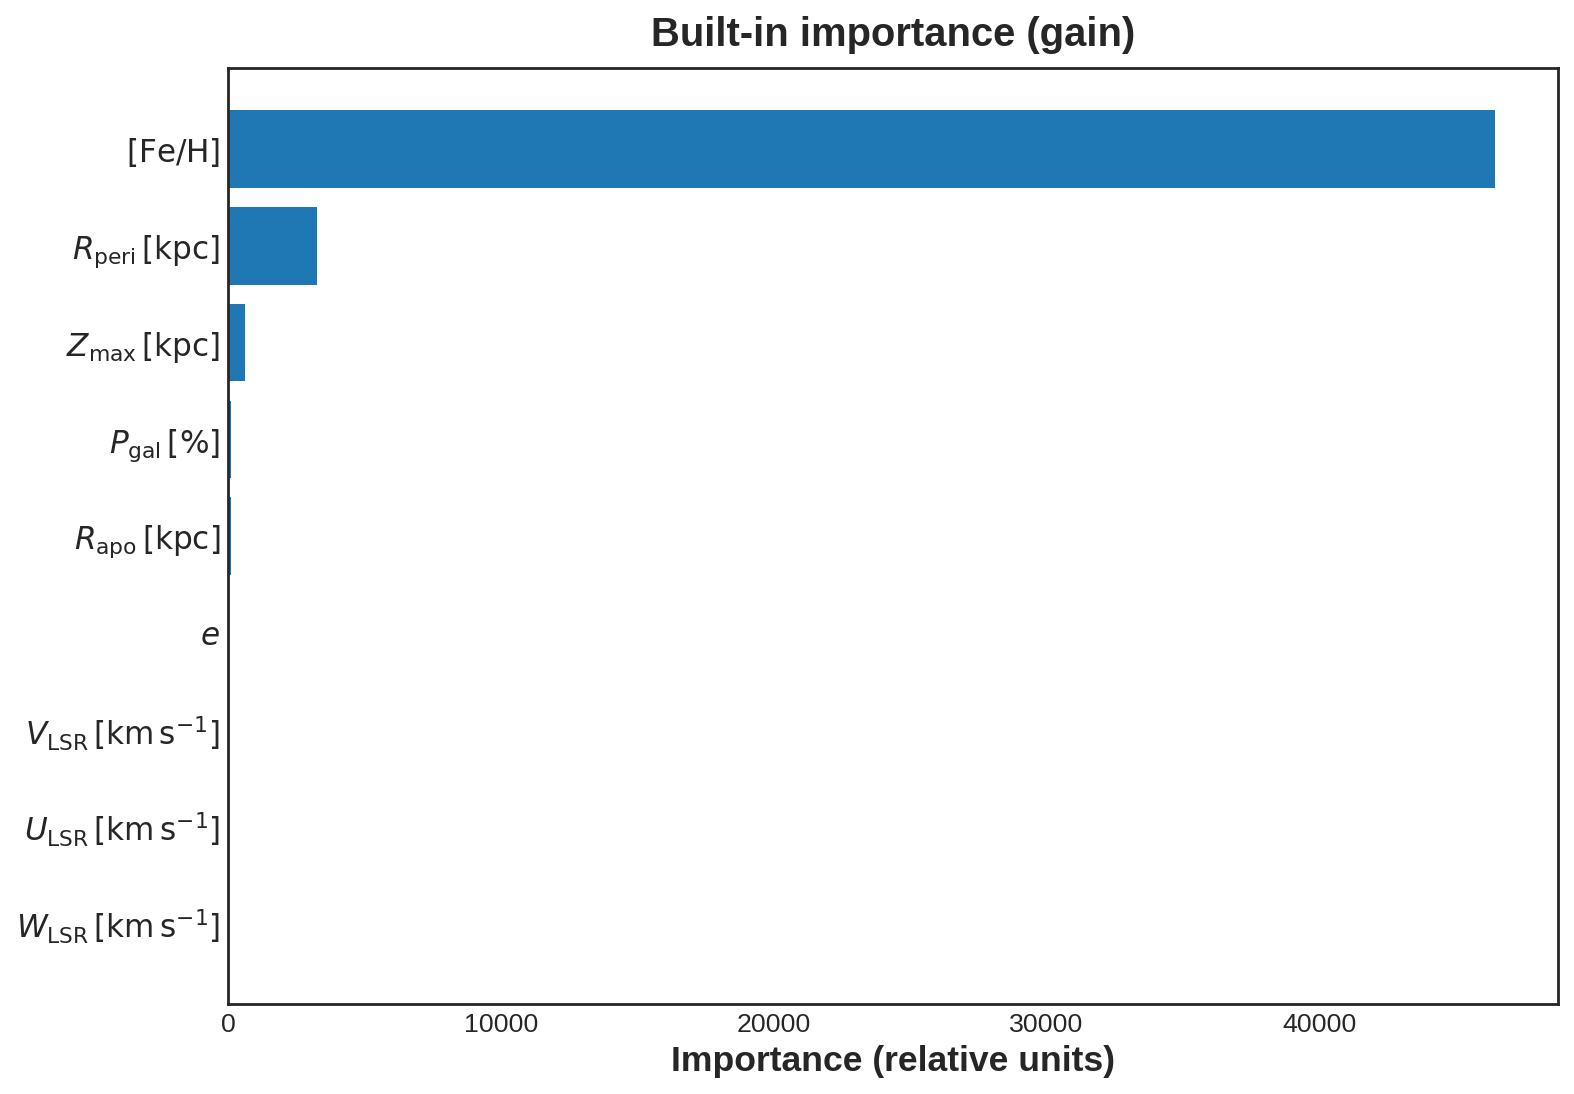
\includegraphics[width=0.24\textwidth]{figures/LGBM_o_h_builtin_gain.png}
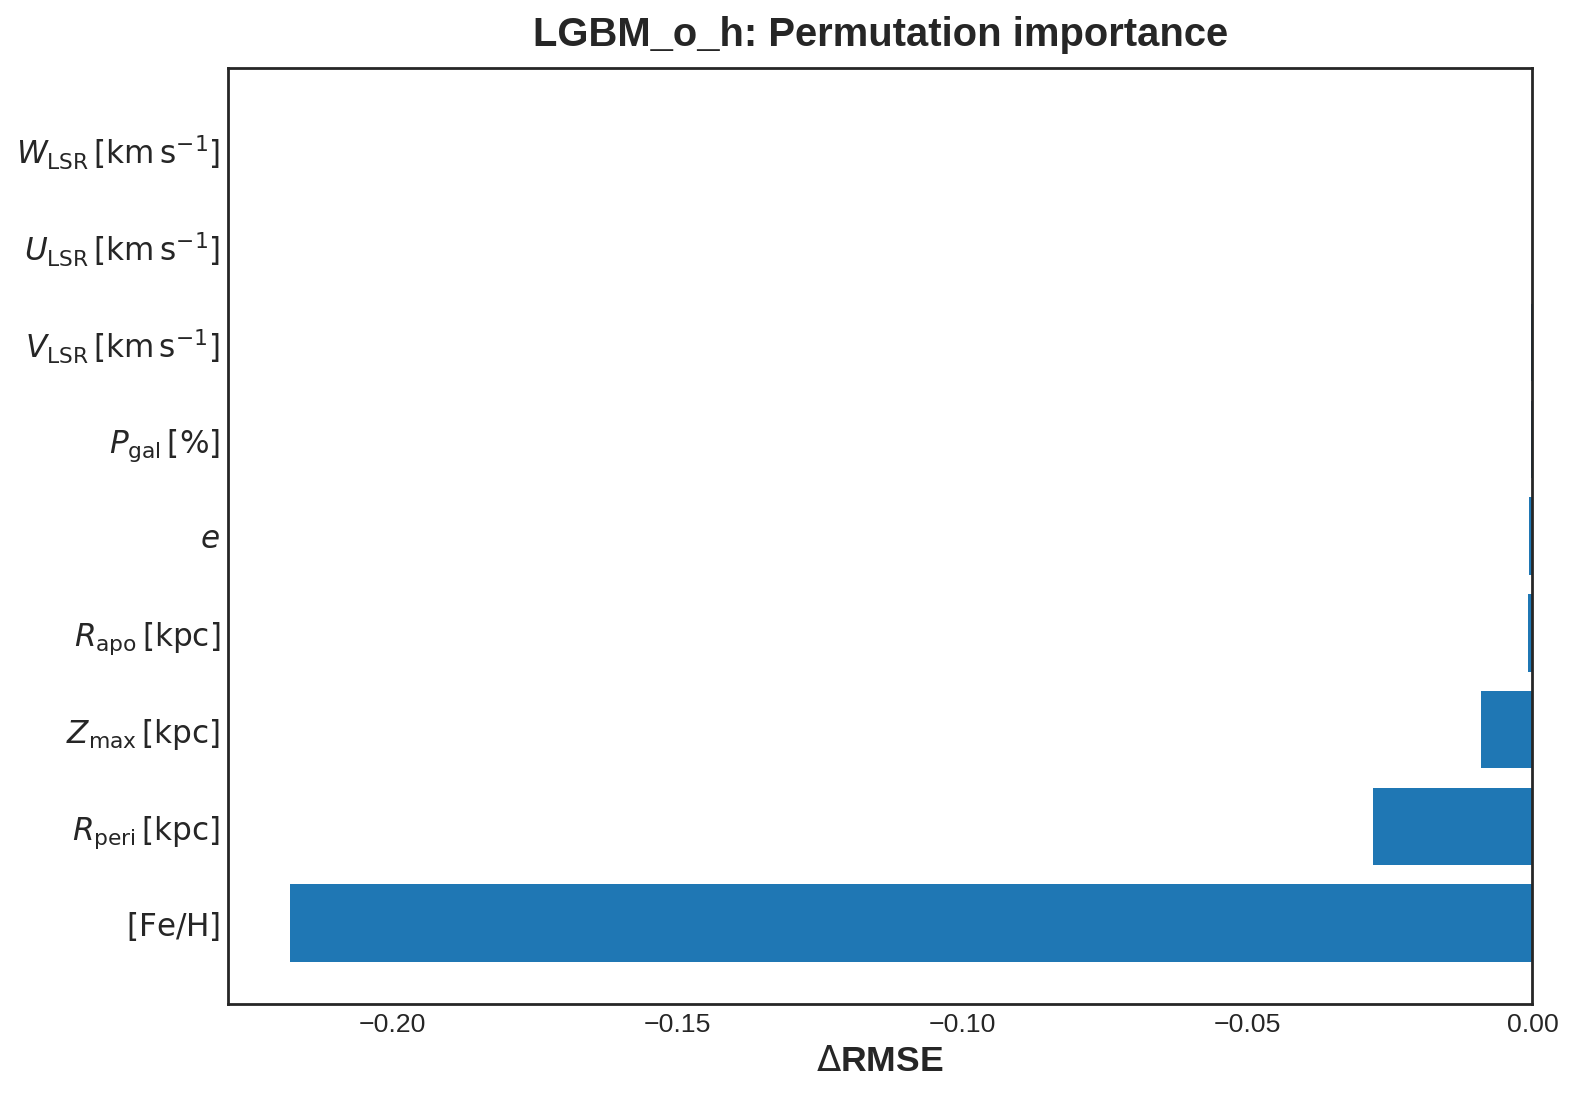
\includegraphics[width=0.24\textwidth]{figures/LGBM_o_h_permutation_dRMSE.png}
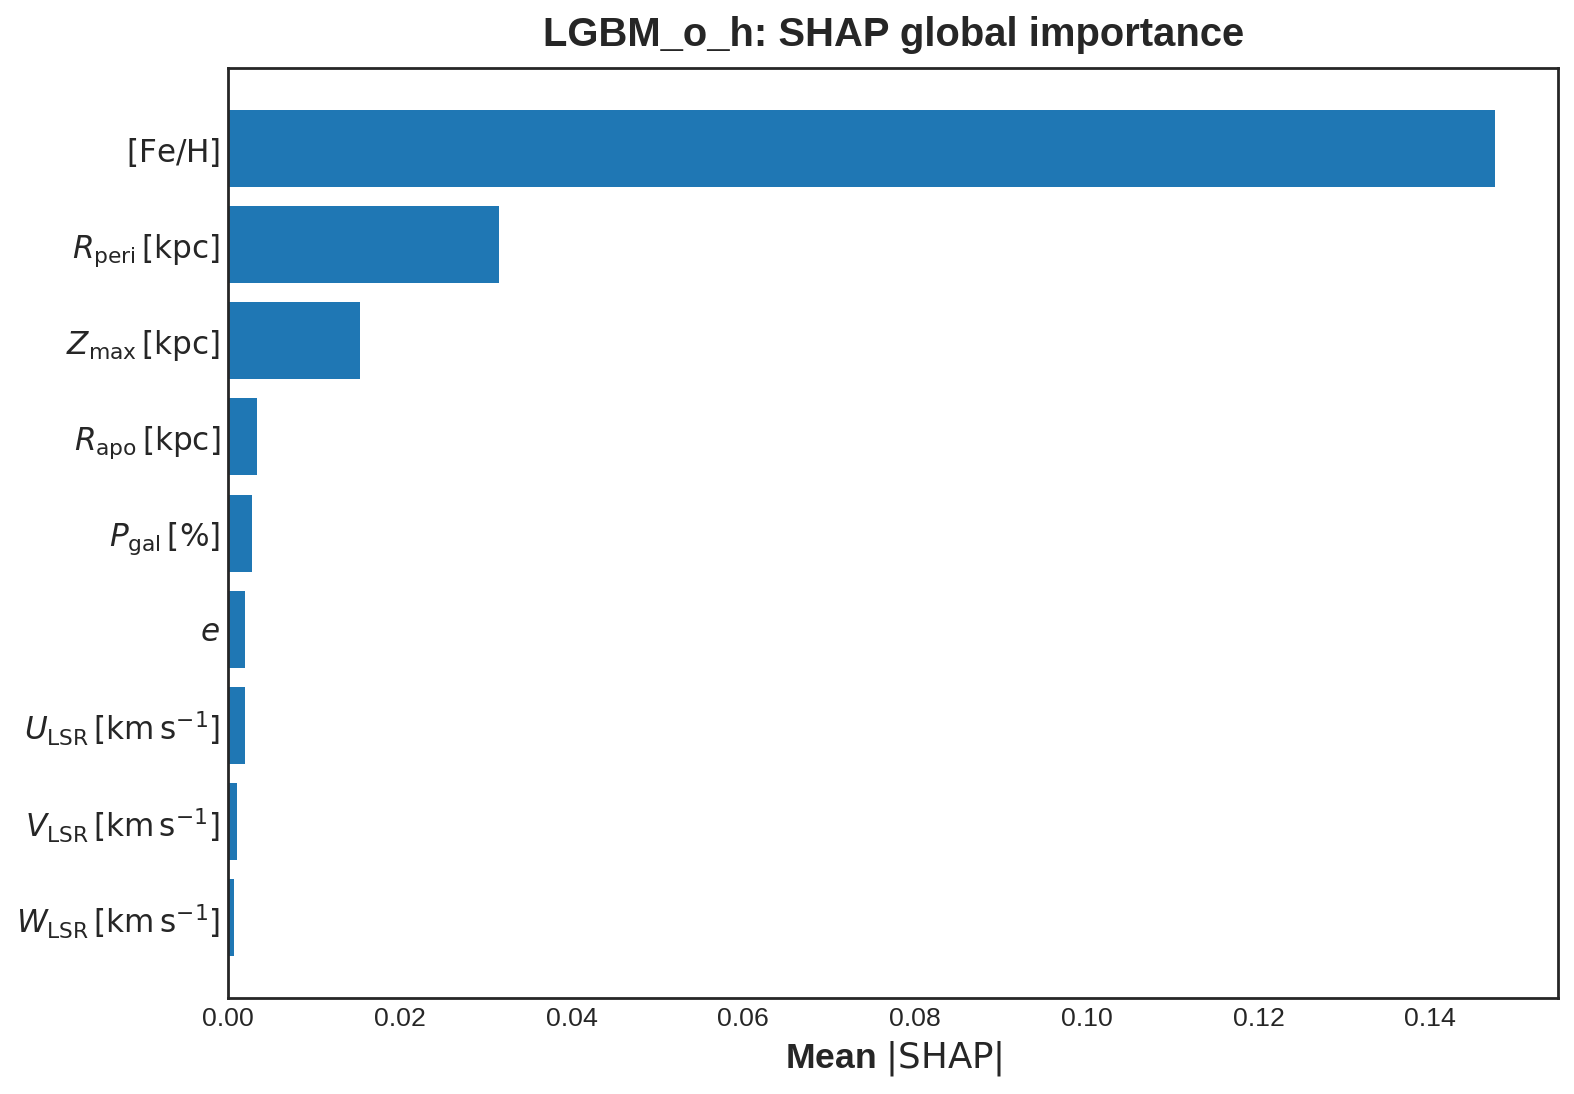
\includegraphics[width=0.24\textwidth]{figures/LGBM_o_h_shap_meanabs.png}
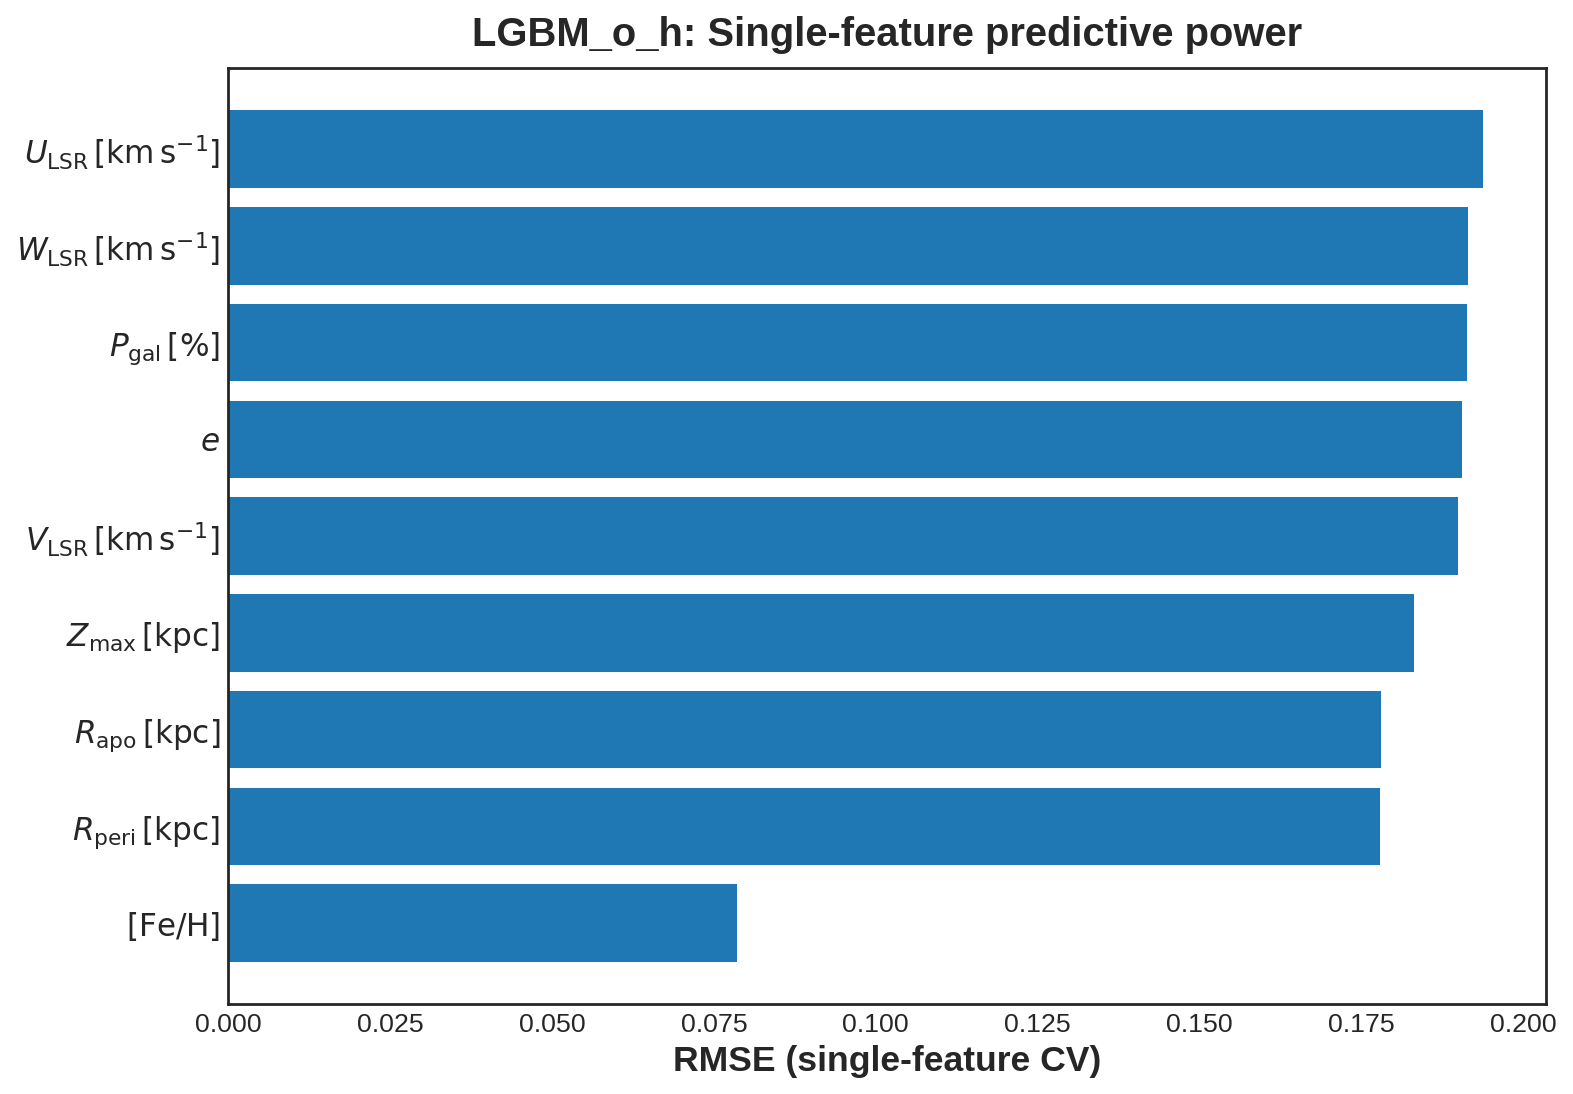
\includegraphics[width=0.24\textwidth]{figures/LGBM_o_h_single_feature_rmse.png}
\caption{Same as Fig.\ref{fig:feature_importance_ch} but for $\mathrm{[O/H]}$}
\label{fig:feature_importance_oh}
\end{figure*}


\begin{figure*}[ht]
\centering
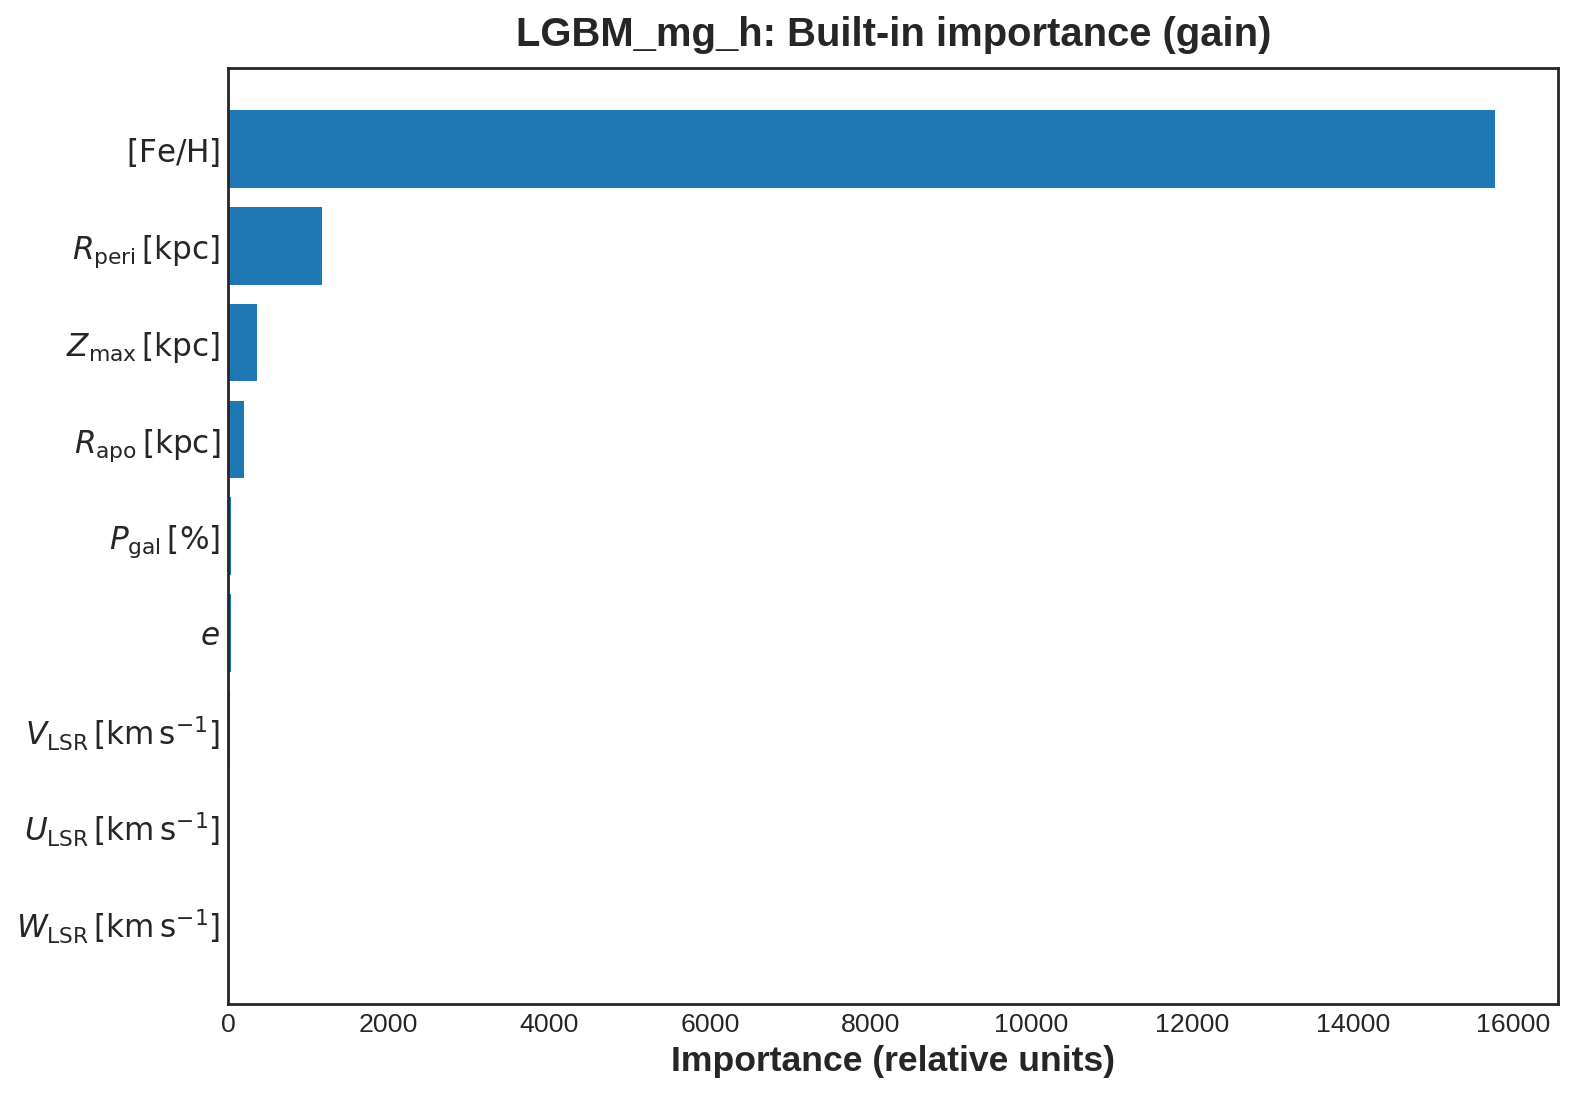
\includegraphics[width=0.24\textwidth]{figures/LGBM_mg_h_builtin_gain.png}
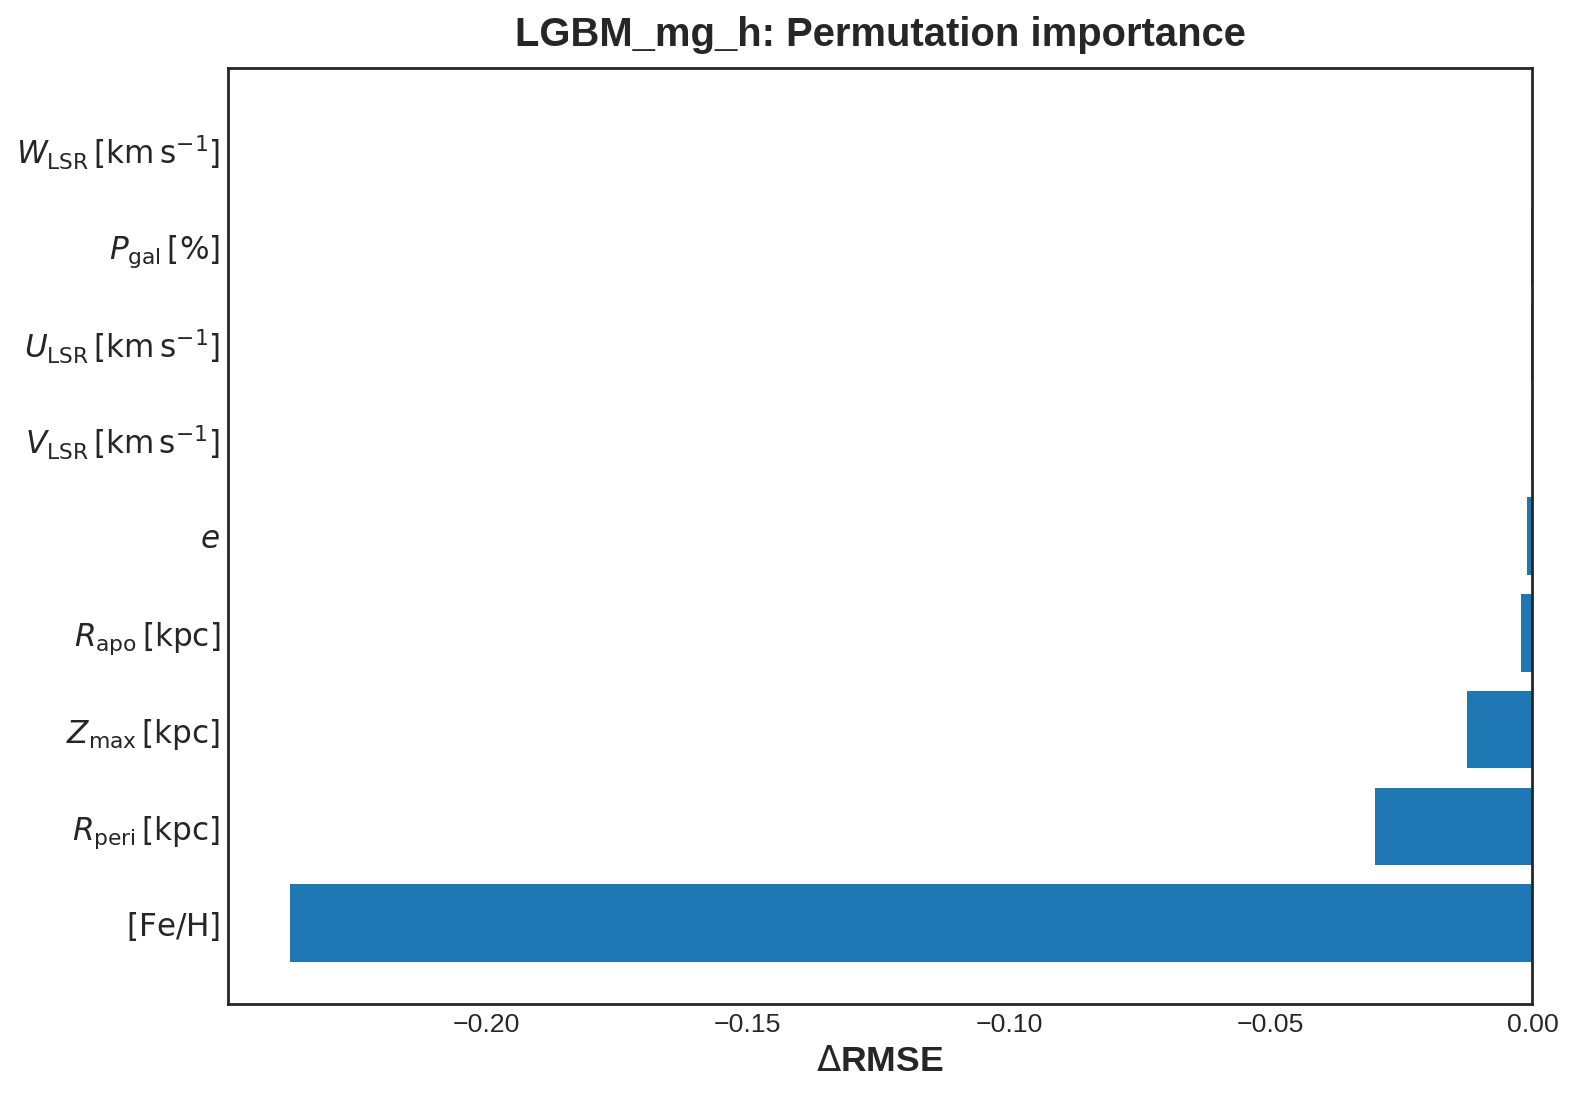
\includegraphics[width=0.24\textwidth]{figures/LGBM_mg_h_permutation_dRMSE.png}
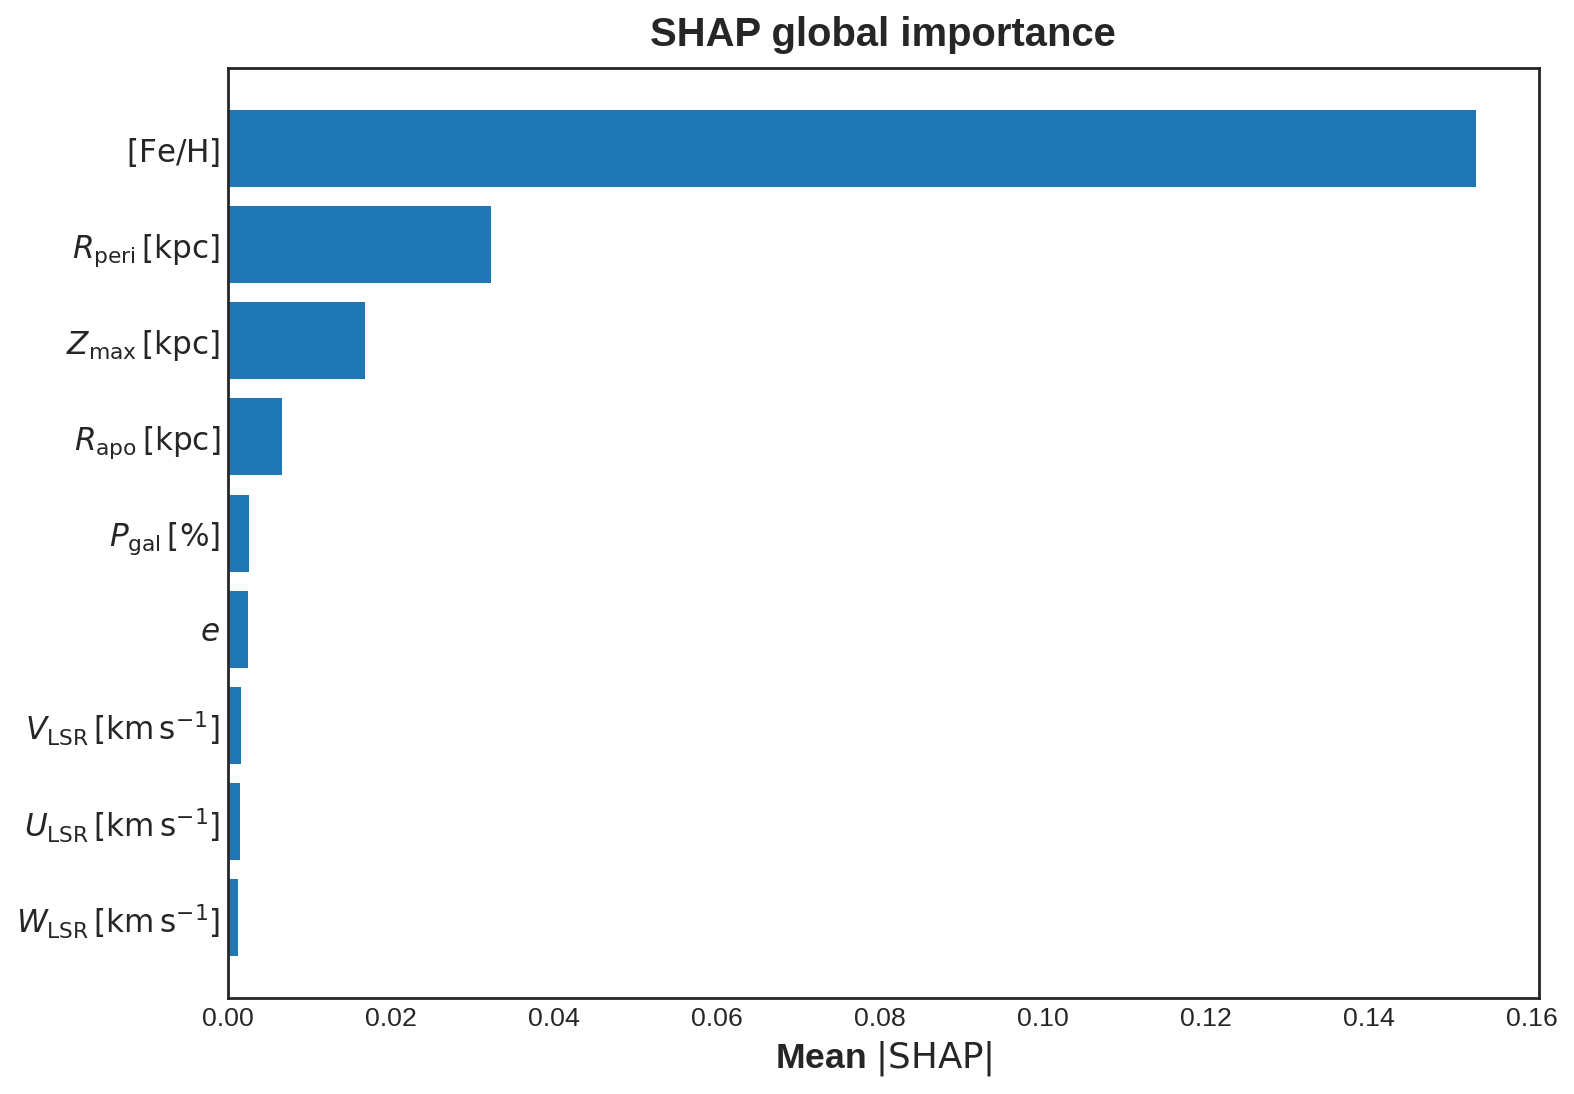
\includegraphics[width=0.24\textwidth]{figures/LGBM_mg_h_shap_meanabs.png}
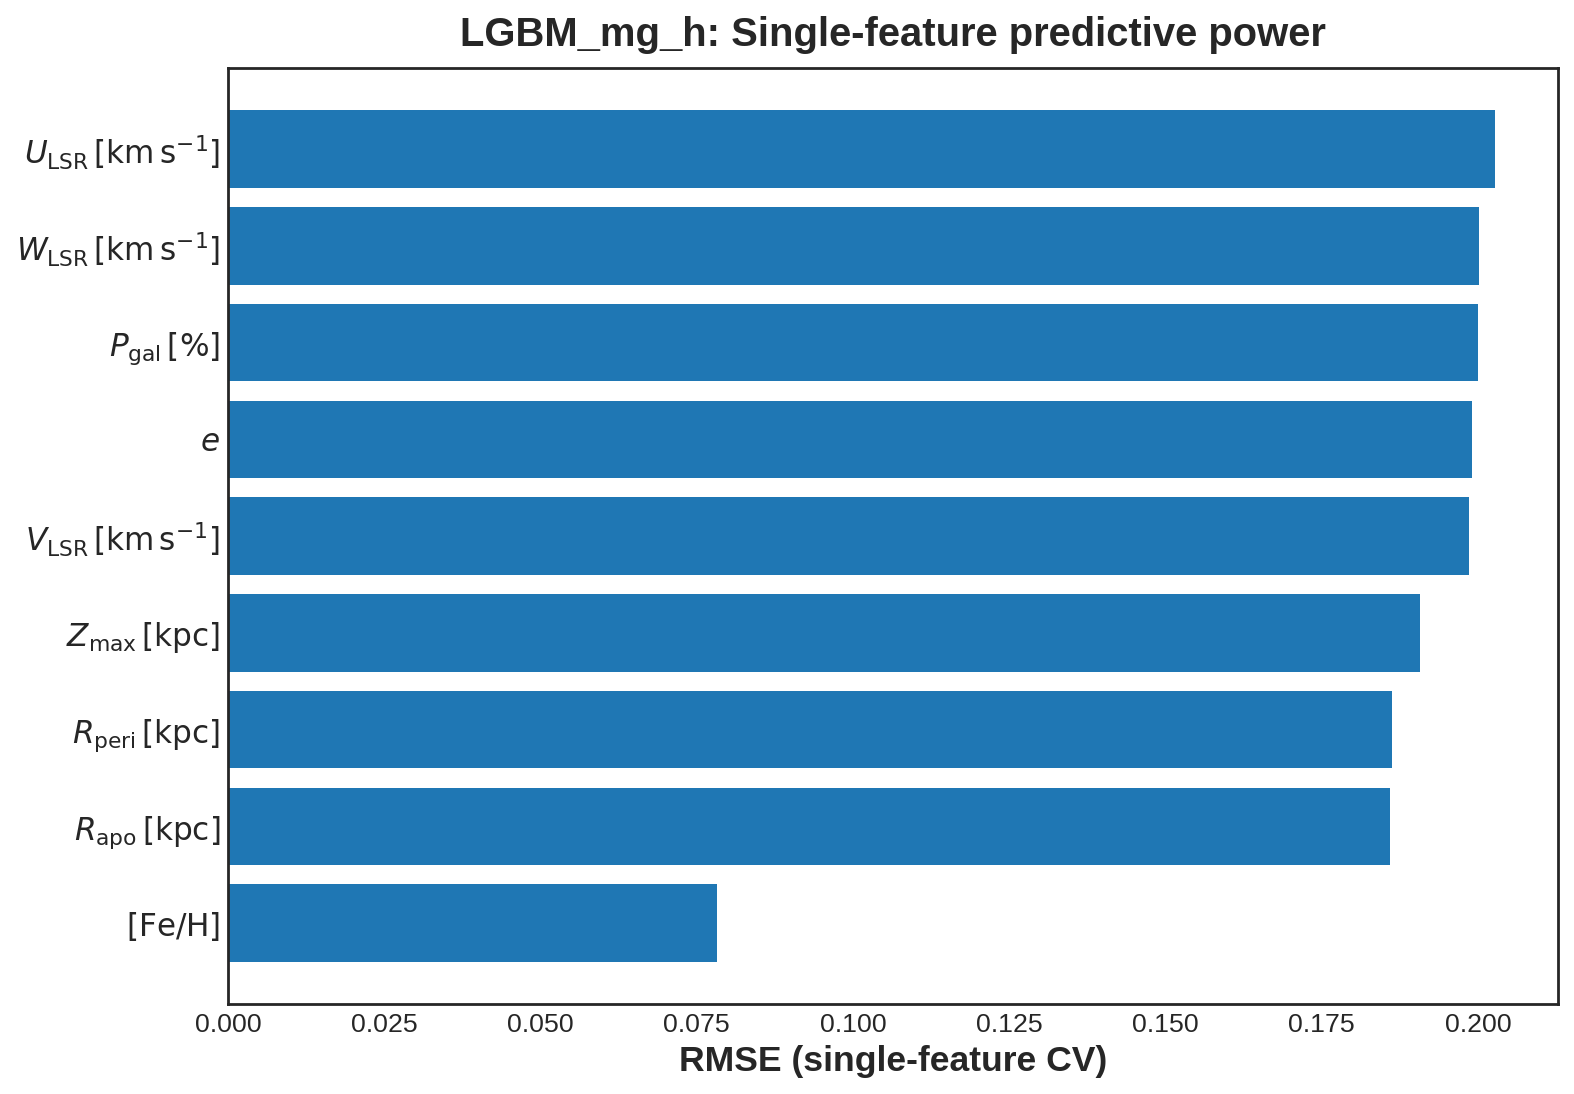
\includegraphics[width=0.24\textwidth]{figures/LGBM_mg_h_single_feature_rmse.png}
\caption{Same as Fig.\ref{fig:feature_importance_ch} but for $\mathrm{[Mg/H]}$}
\label{fig:feature_importance_mgh}
\end{figure*}

\begin{figure*}[ht]
\centering
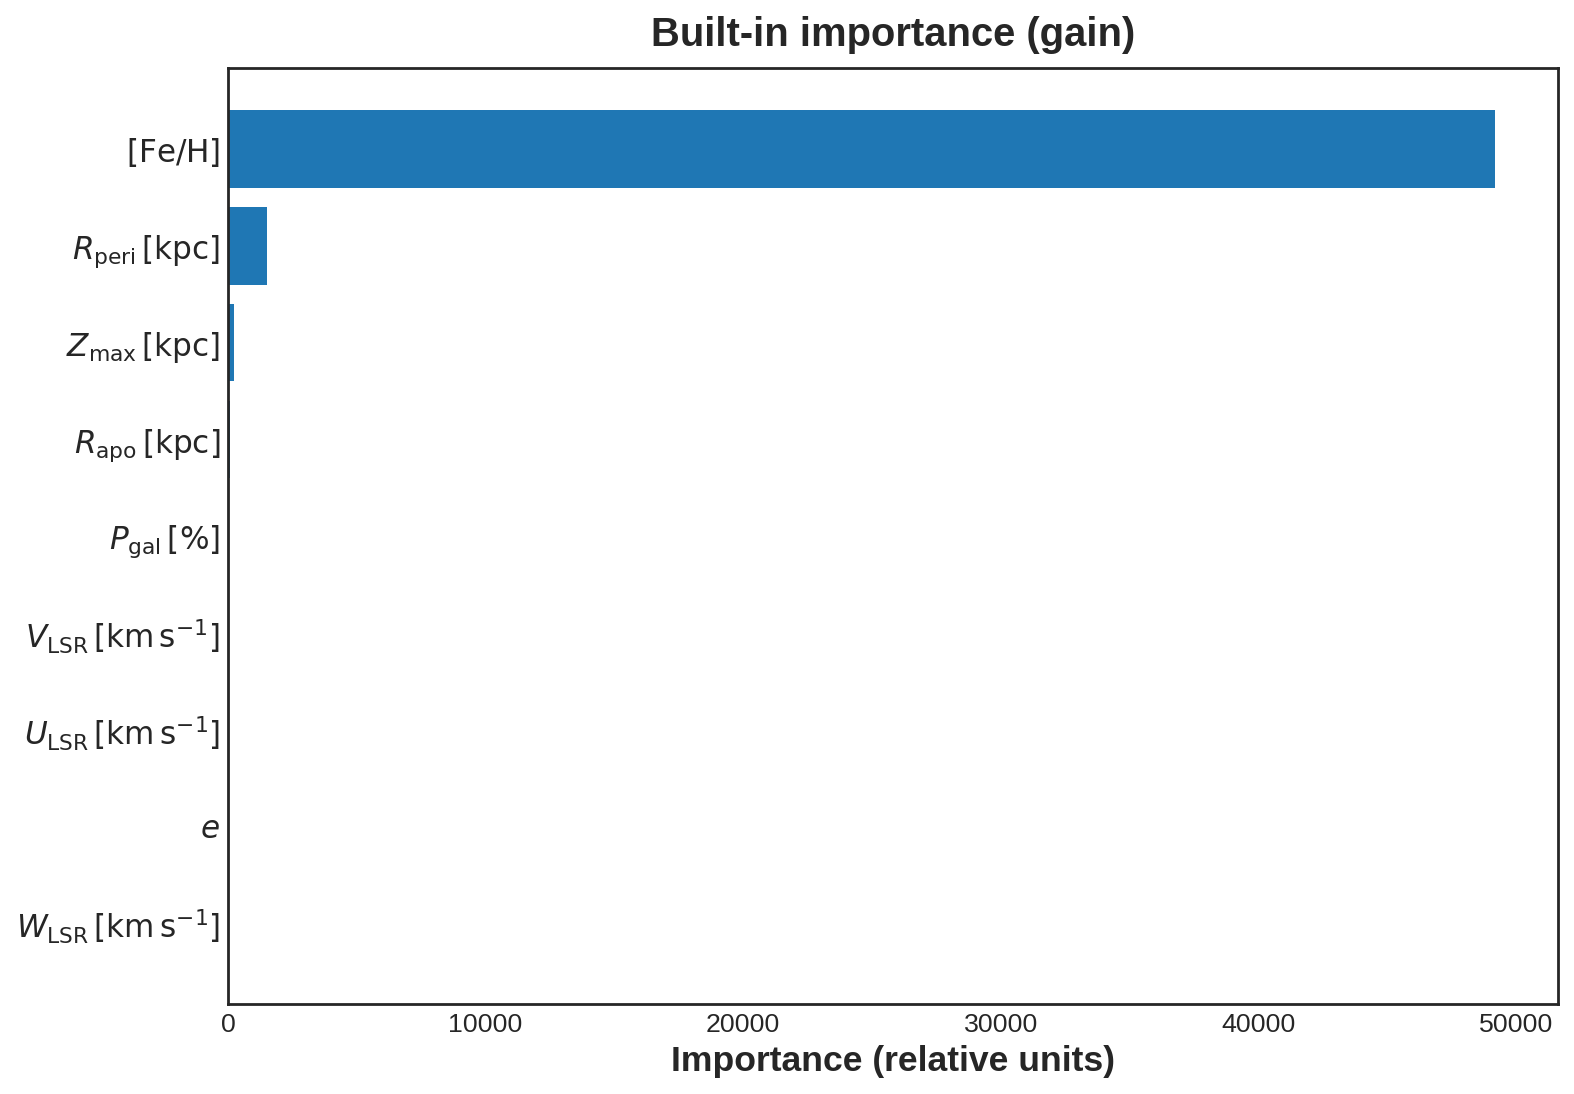
\includegraphics[width=0.24\textwidth]{figures/LGBM_si_h_builtin_gain.png}
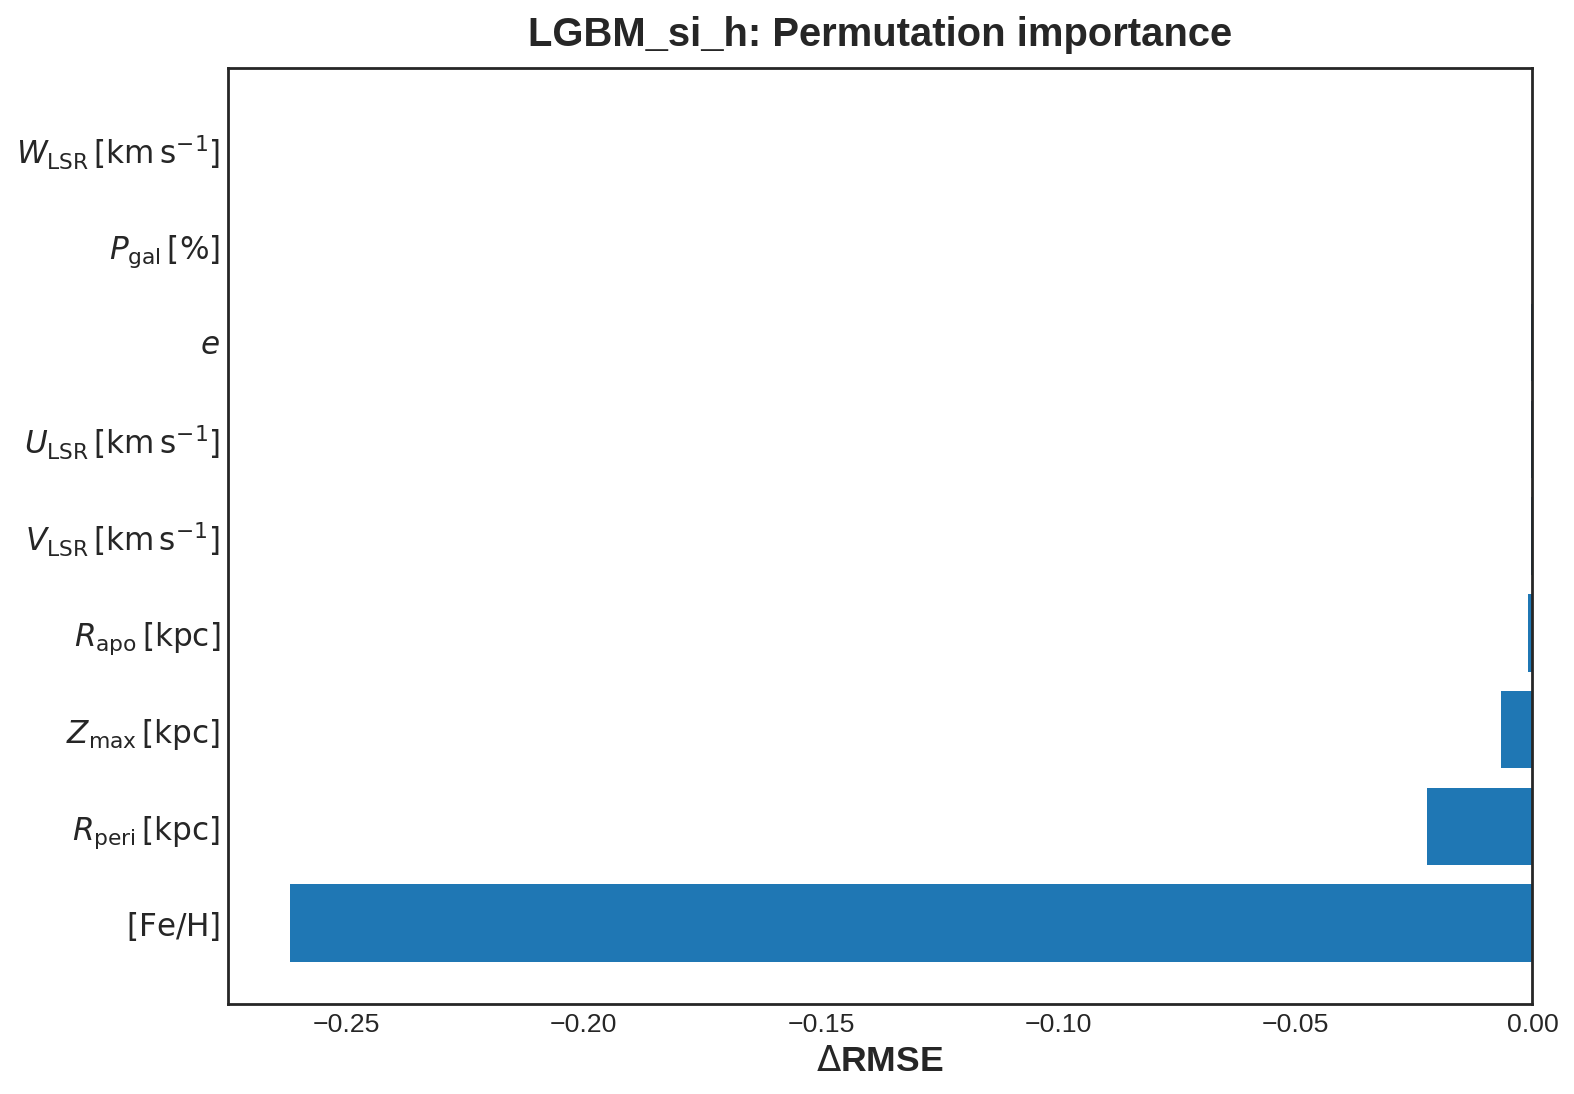
\includegraphics[width=0.24\textwidth]{figures/LGBM_si_h_permutation_dRMSE.png}
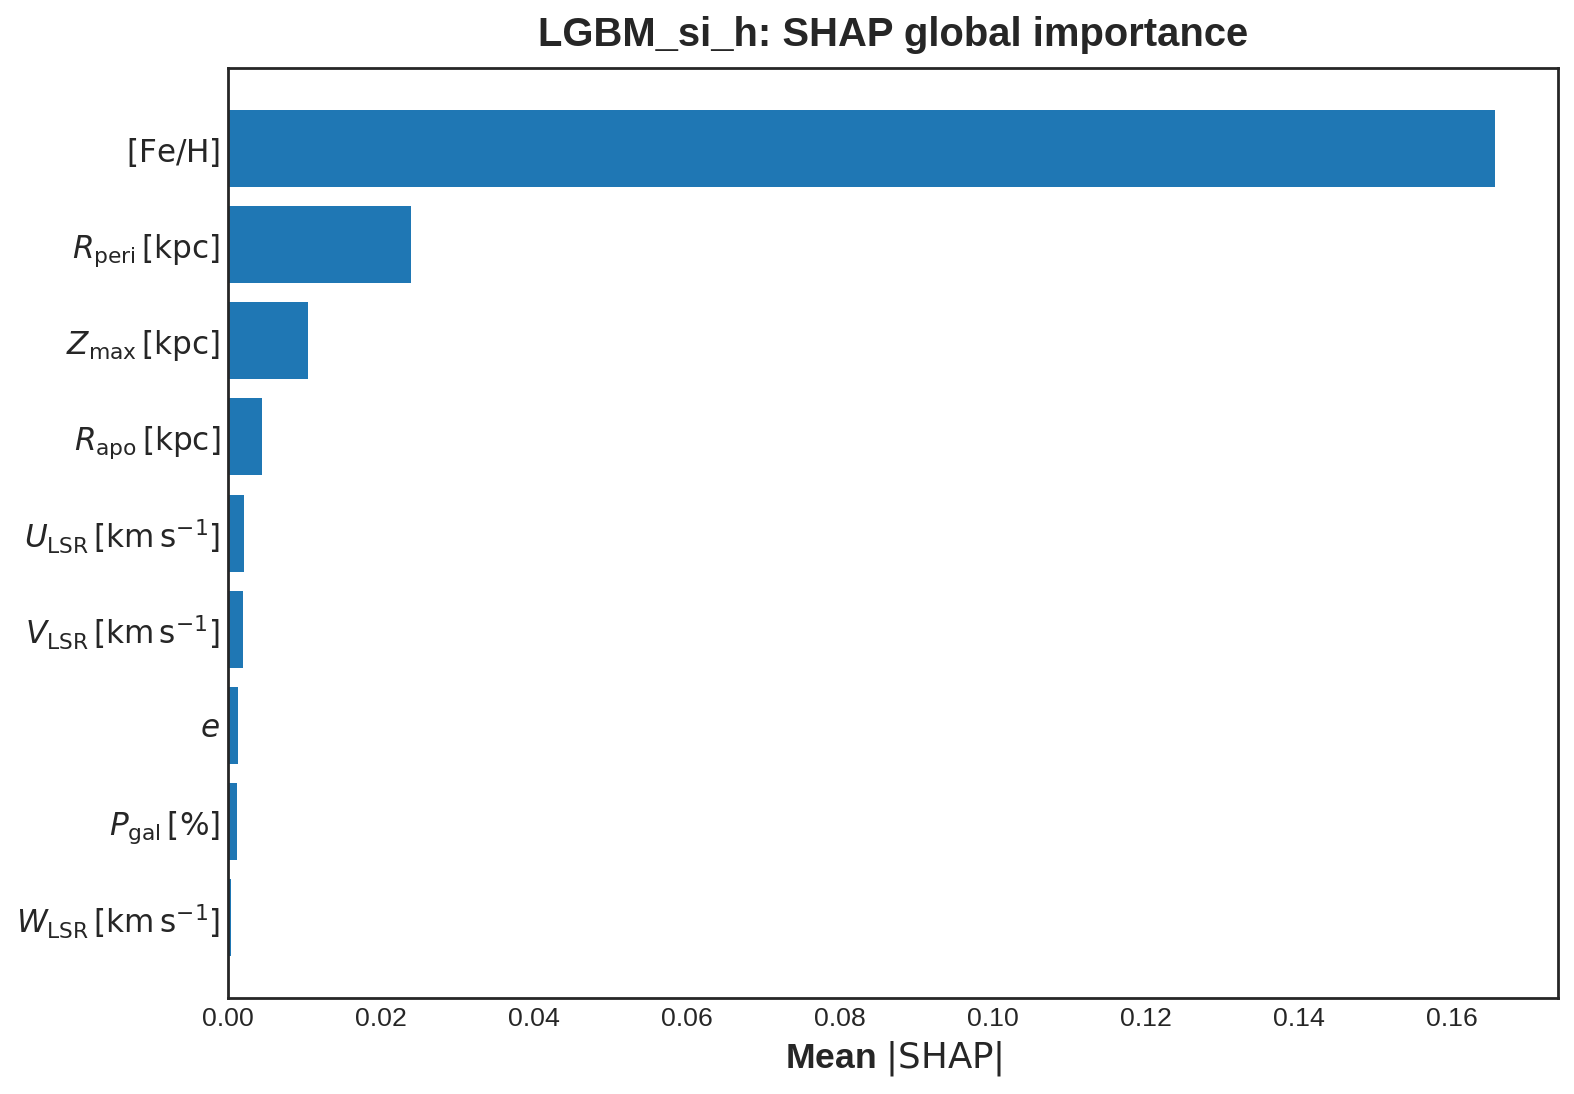
\includegraphics[width=0.24\textwidth]{figures/LGBM_si_h_shap_meanabs.png}
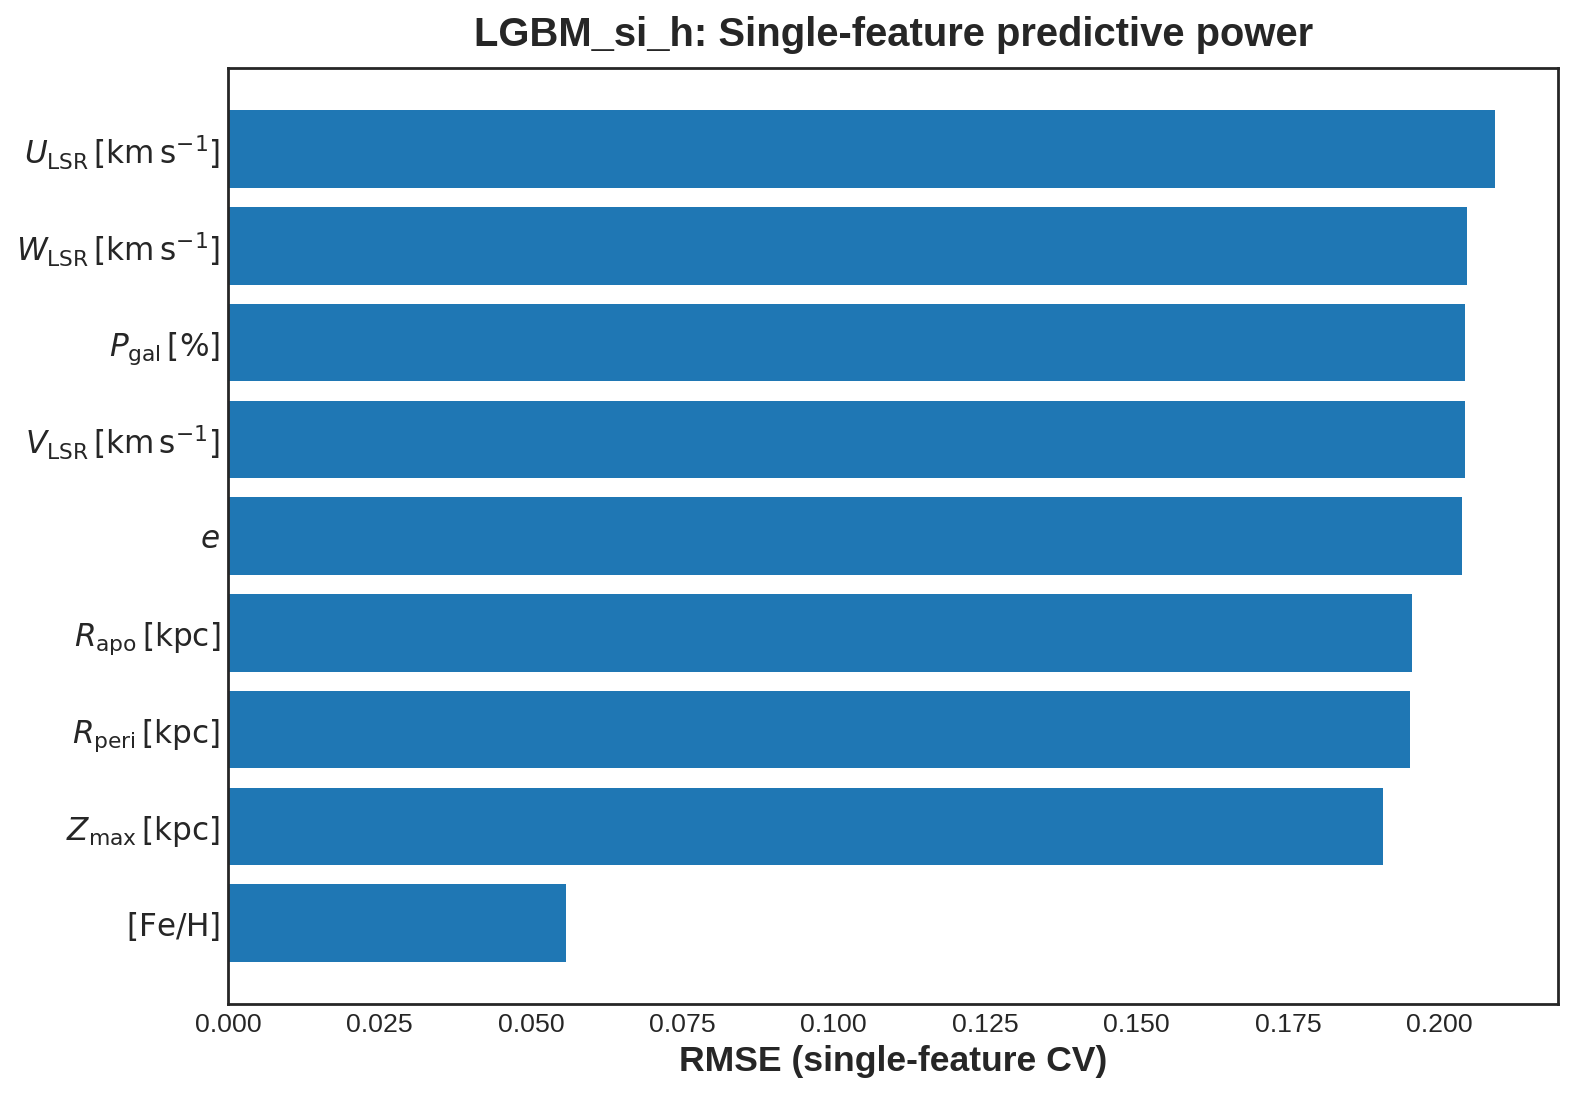
\includegraphics[width=0.24\textwidth]{figures/LGBM_si_h_single_feature_rmse.png}
\caption{Same as Fig.\ref{fig:feature_importance_ch} but for $\mathrm{[Si/H]}$.}
\label{fig:feature_importance_sih}
\end{figure*}

\section{Predicting C and O abundances from Mg, Si and Fe}
\label{appendix:CO_from_MgSiFe}

This appendix presents the full set of feature-importance figures discussed in Sect.~\ref{main_CO_from_MgSiFe}. For completeness, we show the results of the built-in gain importance, permutation importance, SHAP global importance, and single-feature predictive performance for the LightGBM model.

\begin{figure*}[ht]
\centering
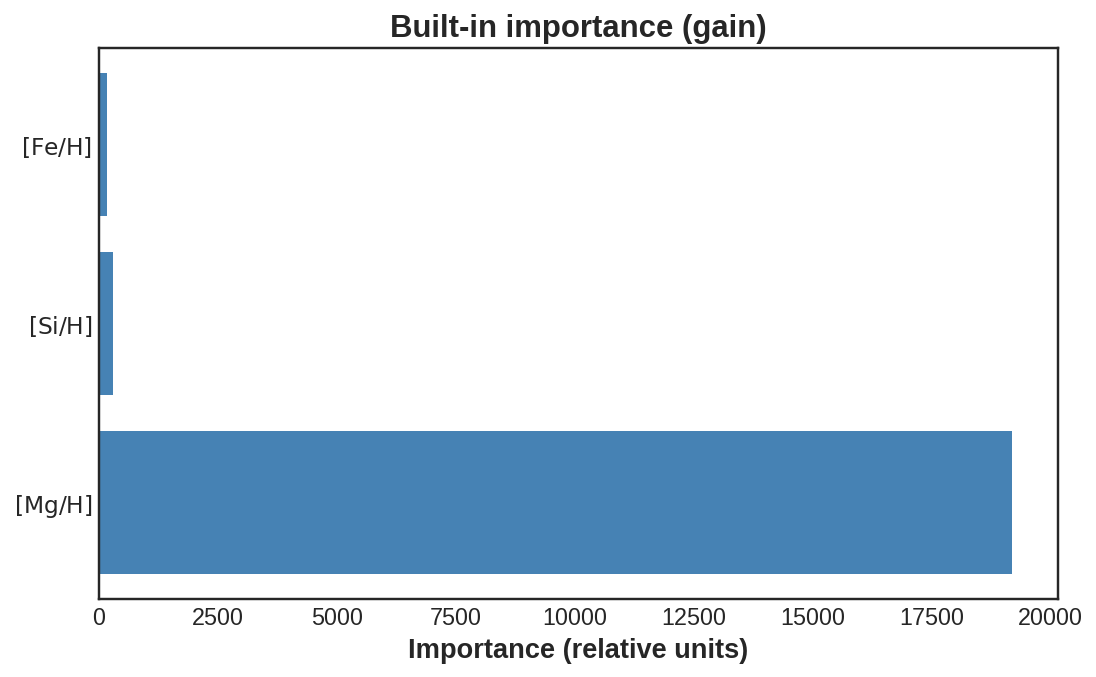
\includegraphics[width=0.24\textwidth]{figures/builtin_gain_fe_mg_si_c_h.png}
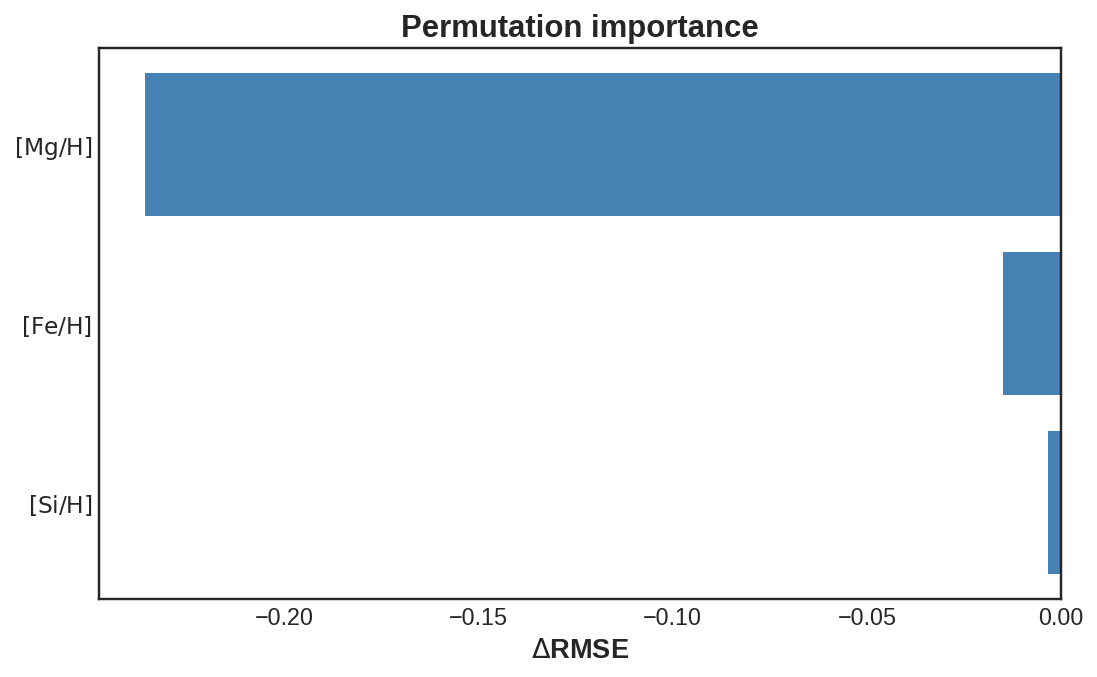
\includegraphics[width=0.24\textwidth]{figures/permutation_drmse_fe_mg_si_c_h.png}
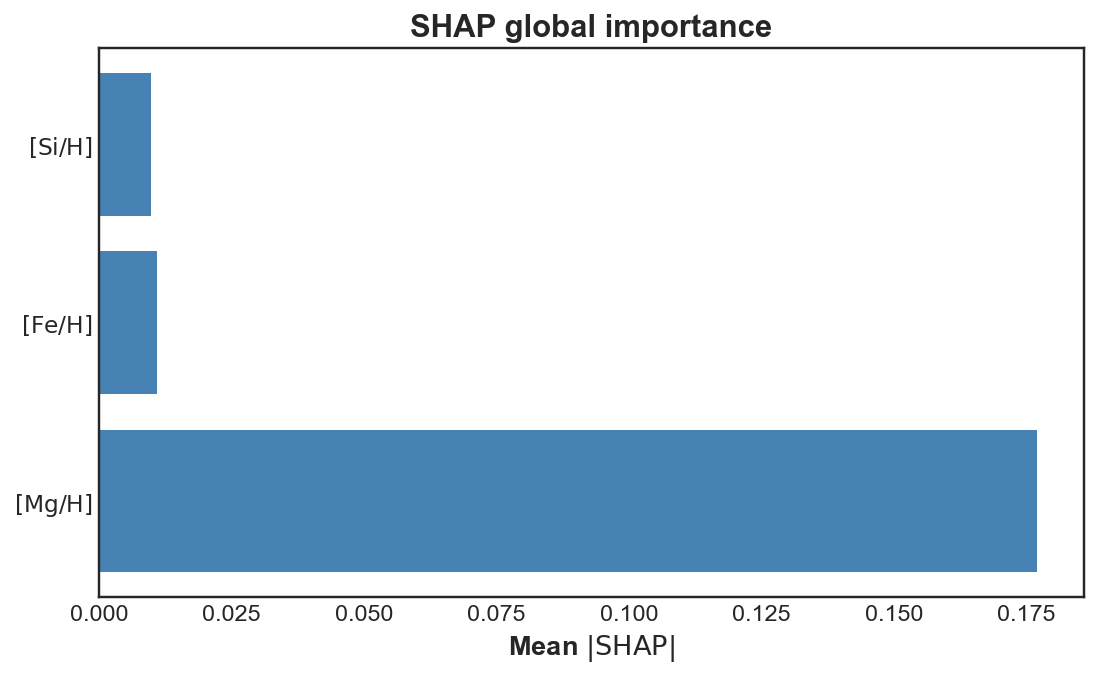
\includegraphics[width=0.24\textwidth]{figures/shap_mean_abs_fe_mg_si_c_h.png}
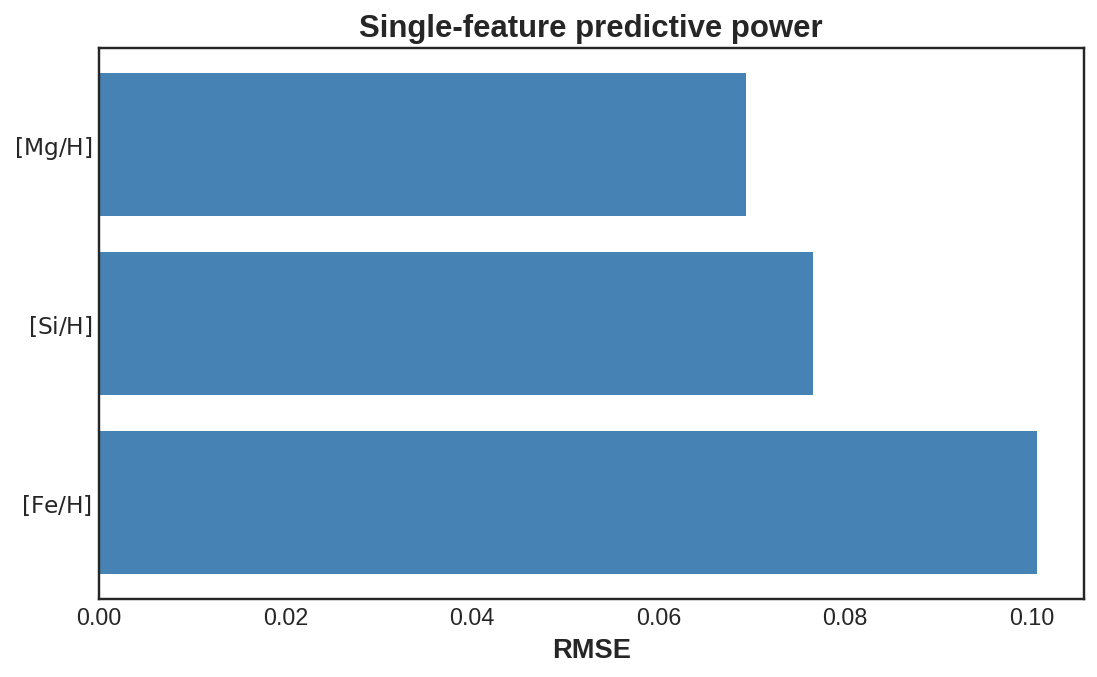
\includegraphics[width=0.24\textwidth]{figures/single_feature_cv_rmse_fe_mg_si_c_h.png}
\caption{Feature-importance diagnostics for the tuned LightGBM model predicting $\mathrm{[C/H]}$ using Mg, Si, and Fe abundances. Built-in gain feature importance derived from the gradient boosting trees (top left). Permutation feature importance, measured as the increase in prediction error ($\Delta$RMSE) after randomly shuffling each feature (top right). Global SHAP importance, showing the mean absolute SHAP value for each feature (bottom left). Predictive performance (RMSE from cross-validation) obtained when training the model using only a single feature at a time (bottom right).}
\label{fig:feature_importance_ch_frommgsife}
\end{figure*}

\begin{figure*}[ht]
\centering
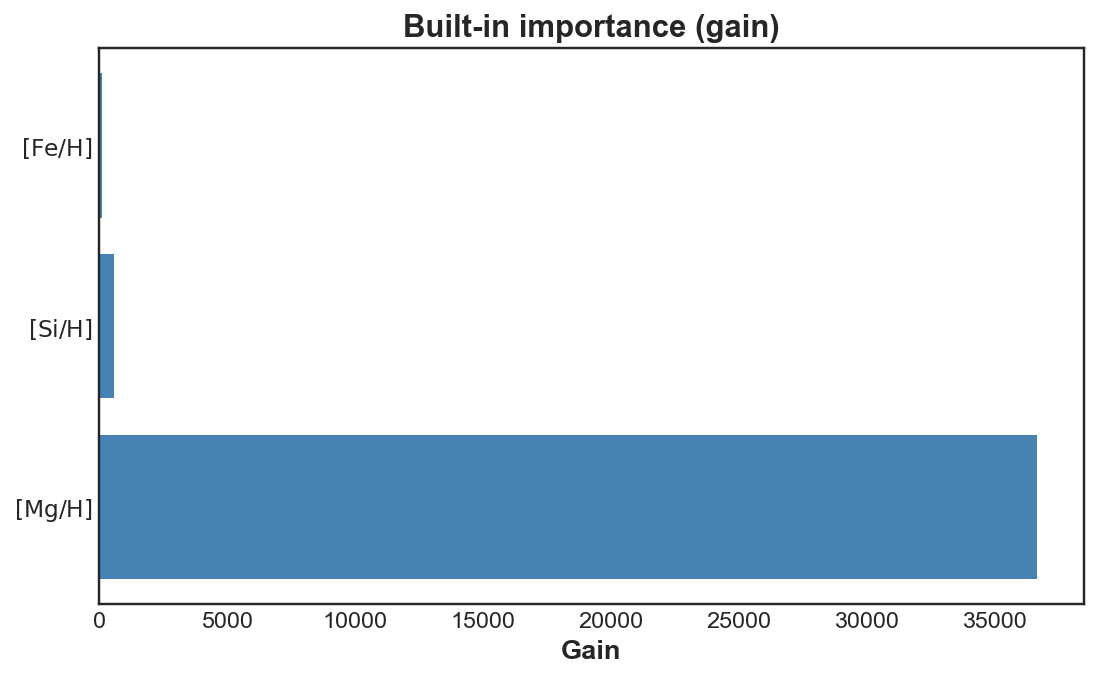
\includegraphics[width=0.24\textwidth]{figures/builtin_gain_fe_mg_si_o_h.png}
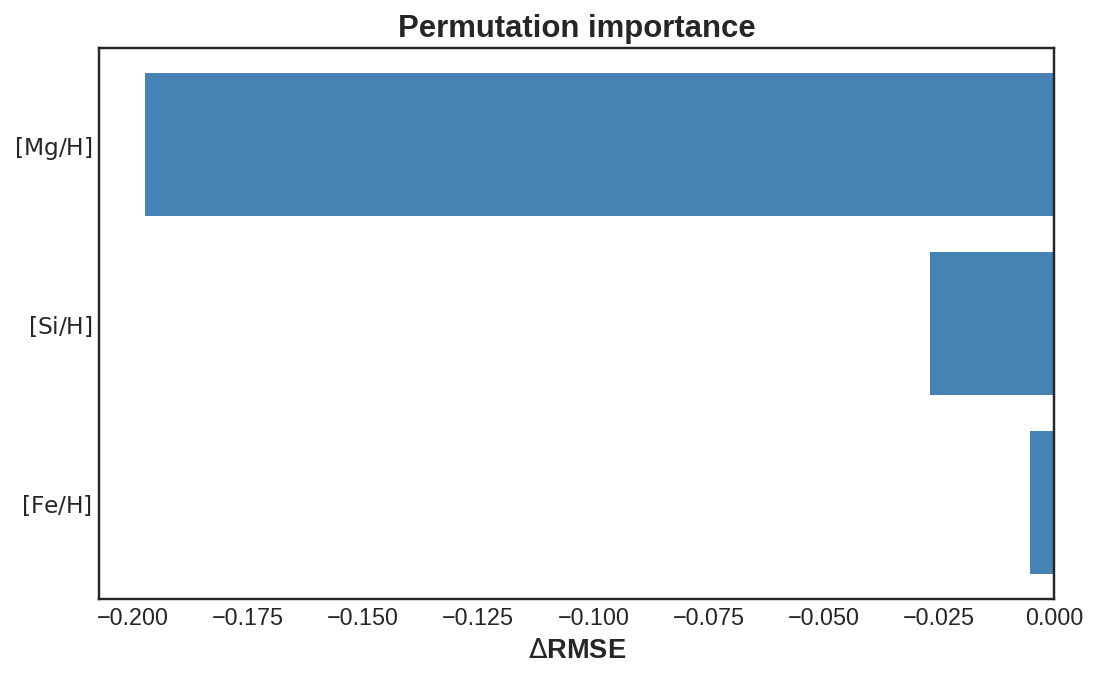
\includegraphics[width=0.24\textwidth]{figures/permutation_drmse_fe_mg_si_o_h.png}
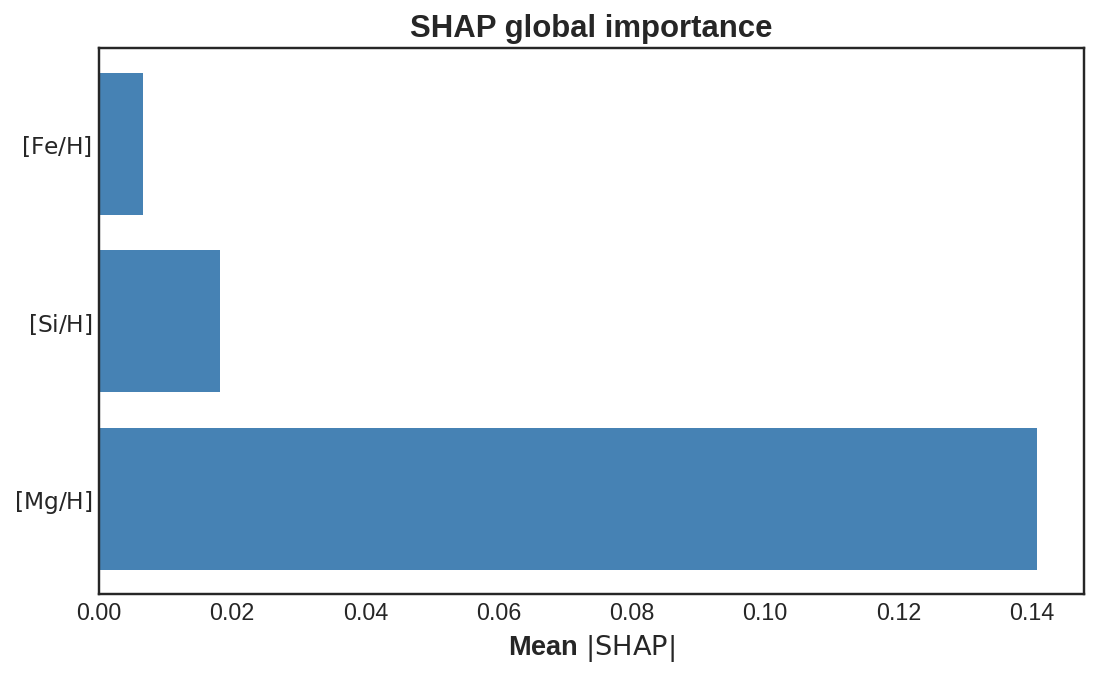
\includegraphics[width=0.24\textwidth]{figures/shap_mean_abs_fe_mg_si_o_h.png}
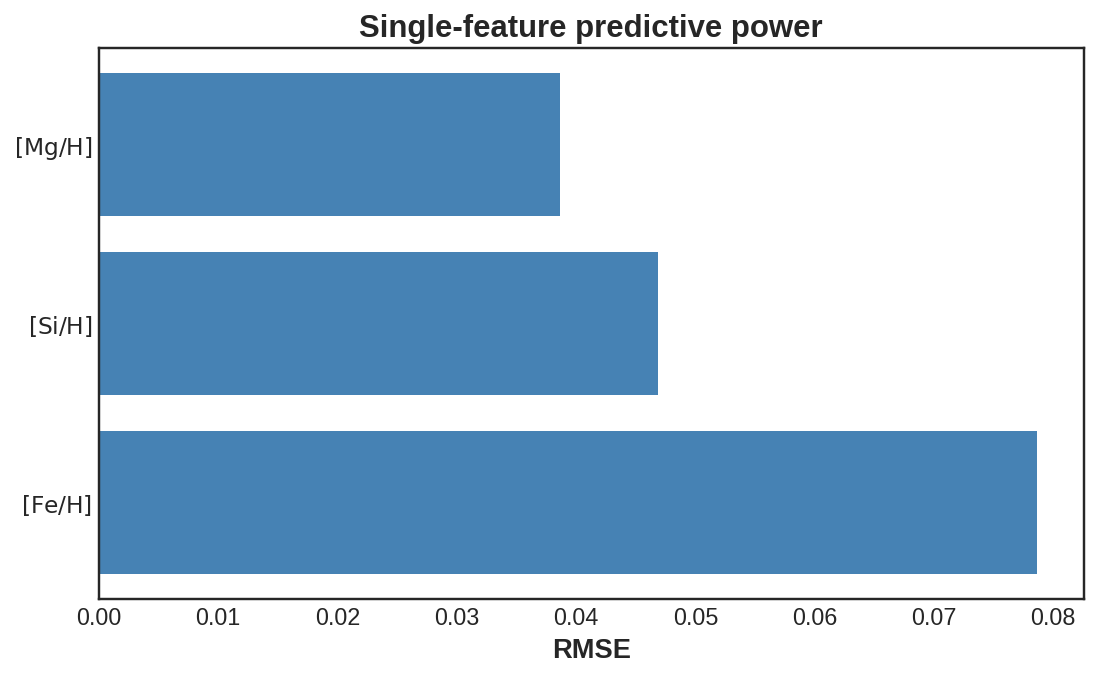
\includegraphics[width=0.24\textwidth]{figures/single_feature_cv_rmse_fe_mg_si_o_h.png}
\caption{Same as Fig.~\ref{fig:feature_importance_ch_frommgsife}, but for $\mathrm{[O/H]}$.}
\label{fig:feature_importance_oh_frommgsife}
\end{figure*}

\end{appendix}
\end{document}
